
%\documentclass[10pt, letterpaper]{article}
\documentclass[10pt, letterpaper]{book}

% package used to set margins, adjust parameters with caution
%\usepackage[left = 0.70in, right = 0.70in, top = 1.0in, bottom = 1.0in]{geometry}
\usepackage[left = 1.10in, right = 1.10in, top = 1.0in, bottom = 0.7in]{geometry}

%%%%%%%%%%%%%%%%%%%%%%%%%%%%%%%%%%%%%%%%%%%%%%
%%%%%%%%%%%%%%%%%%%%%%%%%%%%%%%%%%%%%%%%%%%%%%

% package used to include special header and footer formatting
\usepackage{fancyhdr}

% package used to include special formatting for image and table captions
\usepackage[small,bf,justification=raggedright,format=hang]{caption}

\usepackage{amscd}
\usepackage{amsfonts}
\usepackage{amsmath}
\usepackage{amssymb}
\usepackage{mathrsfs}
\usepackage{bm}

\usepackage{color}
\usepackage[usenames,dvipsnames]{xcolor}
\usepackage{graphicx}
\usepackage{multicol}
\usepackage{verbatim}
%\usepackage{doublespace}
\usepackage{colortbl}
\usepackage{tcolorbox}
\usepackage[shortlabels]{enumitem}

\usepackage{epsfig}
\usepackage{tikz-cd}

%%%%%%%%%%%%%%%%%%%%%%%%%%%%%%%%%%%%%%%%%%%%%%
%%%%%%%%%%%%%%%%%%%%%%%%%%%%%%%%%%%%%%%%%%%%%%
\renewcommand{\theenumi}{\arabic{enumi}}
\renewcommand{\labelenumi}{\mbox{}\;\theenumi.$\;$}

\renewcommand{\theenumii}{\alph{enumii}}
%\renewcommand{\labelenumii}{\mbox{}{\color{white}.}\;\;\;\;{\color{white}.}(\theenumii)$\quad$}
\renewcommand{\labelenumii}{\textnormal{(\theenumii)$\quad$}}
\setlist[enumerate,2]{leftmargin=1.05cm}

\renewcommand{\theenumiii}{\roman{enumiii}}
\renewcommand{\labelenumiii}{\mbox{}\;\;\,\theenumiii)$\quad$}

\renewcommand{\theequation}{\thesection .\arabic{equation}}

\newcounter{theorem}

\newtheorem{example}[theorem]{Example}
\renewcommand{\theexample}{ \thesection .\arabic{example}}

\newtheorem{definition}[theorem]{Definition}
\renewcommand{\thedefinition}{\thesection .\arabic{definition}}

\newtheorem{theorem}[theorem]{Theorem}
\renewcommand{\thetheorem}{\thesection .\arabic{theorem}}

\newtheorem{proposition}[theorem]{Proposition}
\renewcommand{\theproposition}{\thesection .\arabic{proposition}}

\newtheorem{conjecture}[theorem]{Conjecture}
\renewcommand{\theconjecture}{\thesection .\arabic{conjecture}}

\newtheorem{lemma}[theorem]{Lemma}
\renewcommand{\thelemma}{\thesection .\arabic{lemma}}

\newtheorem{corollary}[theorem]{Corollary}
\renewcommand{\thecorollary}{\thesection .\arabic{corollary}}

\newtheorem{remark}[theorem]{Remark}
\renewcommand{\theremark}{\thesection .\arabic{remark}}

\newtheorem{notation}[theorem]{Notation}
\renewcommand{\thenotation}{\thesection .\arabic{notation}}

\renewcommand{\thetable} {\thesection .\arabic{table}}

\renewcommand{\thefigure}{\thesection .\arabic{figure}}

%%%%%%%%%%%%%%%%%%%%%%%%%%%%%%%%%%%%%%%%%%%%%%
%%%%%%%%%%%%%%%%%%%%%%%%%%%%%%%%%%%%%%%%%%%%%%
\DeclareFontFamily{U}{mathx}{}
\DeclareFontShape{U}{mathx}{m}{n}{<-> mathx10}{}
\DeclareSymbolFont{mathx}{U}{mathx}{m}{n}
%\DeclareMathAccent{\widehat}{0}{mathx}{"70}
\DeclareMathAccent{\widecheck}{0}{mathx}{"71}

\newcommand*{\proof}{\noindent {\small P{\scriptsize ROOF}} \quad}
\newcommand*{\proofof}{\noindent {\small P{\scriptsize ROOF OF }}}
\newcommand*{\proofoutline}{\noindent {\small O{\scriptsize UTLINE OF PROOF}} \quad}
\newcommand*{\proofoutlineof}{\noindent {\small O{\scriptsize UTLINE OF PROOF OF }}}
\newcommand*{\qed}{\hfill $\Box$}
\newcommand*{\hdiamond}{\hfill $\Diamond$}

\renewcommand*{\Re}{\mathbb{R}}
\renewcommand*{\d}{\textnormal{d}}
\newcommand{\C}{\mathbb{C}}
\newcommand{\Q}{\mathbb{Q}}
\newcommand{\N}{\mathbb{N}}
\newcommand{\Z}{\mathbb{Z}}
\newcommand{\F}{\mathbb{F}}
\newcommand{\varemptyset}{\varnothing}
\renewcommand{\i}{\textnormal{\bf i}}

\newcommand{\diag}{\textnormal{diag}}
\newcommand{\proj}{\textnormal{proj}}
\newcommand{\rot}{\textnormal{rot}}

\newcommand{\ev}{\textnormal{ev}}
\newcommand{\rank}{\textnormal{rank}}
\renewcommand*{\span}{\textnormal{span}}
\newcommand*{\domain}{\textnormal{domain}}
\newcommand*{\codomain}{\textnormal{codomain}}
\newcommand{\Col}{\textnormal{Col}}
\newcommand{\image}{\textnormal{image}}
\newcommand{\Var}{\textnormal{Var}}
%\newcommand{\Hess}{\textnormal{Hess}}
\newcommand{\Hess}{\nabla^{2}}
\newcommand{\Cov}{\textnormal{Cov}}
\newcommand{\MSE}{\textnormal{MSE}}
\newcommand{\SVar}{\textnormal{SVar}}

\newcommand*{\longhookrightarrow}{\ensuremath{\lhook\joinrel\relbar\joinrel\rightarrow}}

%\newcommand{\Czo}{C([0,1],\Re)}
\newcommand{\Czo}{C[0,1]}

\newcommand{\logisticBetaX}{
	\dfrac{\exp\!\left(\,\beta^{T} \cdot x \,\right)}{1 \,+\, \exp\!\left(\,\beta^{T} \cdot x \,\right)}
}

\newcommand{\oneMinusLogisticBetaX}{
	\dfrac{1}{1 \,+\, \exp\!\left(\,\beta^{T} \cdot x \,\right)}
}

\newcommand{\argmin}{\textnormal{argmin}}
\newcommand{\argmax}{\textnormal{argmax}}

%%%%%%%%%%%%%%%%%%%%%%%%%%%%%%%%%%%%%%%%%%%%%%
%%%%%%%%%%%%%%%%%%%%%%%%%%%%%%%%%%%%%%%%%%%%%%

\begin{document}

%%%%%%%%%%%%%%%%%%%%%%%%%%%%%%%%%%%%%%%%%%%%%%

\pagecolor{black}

%\definecolor{titlepagetext}{RGB}{255,191,0}
\definecolor{titlepagetext}{RGB}{255,200,0}

%%%%%%%%%%

\begin{titlepage}
\begin{center}
\vspace*{0.8cm}

\resizebox{0.7\linewidth}{!}{\bf\itshape\color{titlepagetext}Mathematical Structure}
\vskip 0.5cm
\textbf{\color{titlepagetext}\fontsize{40}{43}\selectfont\itshape of the}
\vskip 0.3cm
\resizebox{0.8\linewidth}{!}{\bf\itshape\color{titlepagetext}Standard Model}
\vskip 0.4cm
\textbf{\color{titlepagetext}\fontsize{50}{53}\selectfont\itshape of}
\vskip 0.3cm
\resizebox{0.8\linewidth}{!}{\bf\itshape\color{titlepagetext}Particle Physics}
            
\vspace{0.5cm}
\Huge
\textbf{\color{titlepagetext}Kenneth Chu}

\vspace{0.9cm}
%\includegraphics[width=0.99\textwidth]{graphics/090516_standardmodel_2.jpg}
%\includegraphics[width=0.99\textwidth]{graphics/HT_proton_collision_nt_130703_33x16_1600.jpg}
%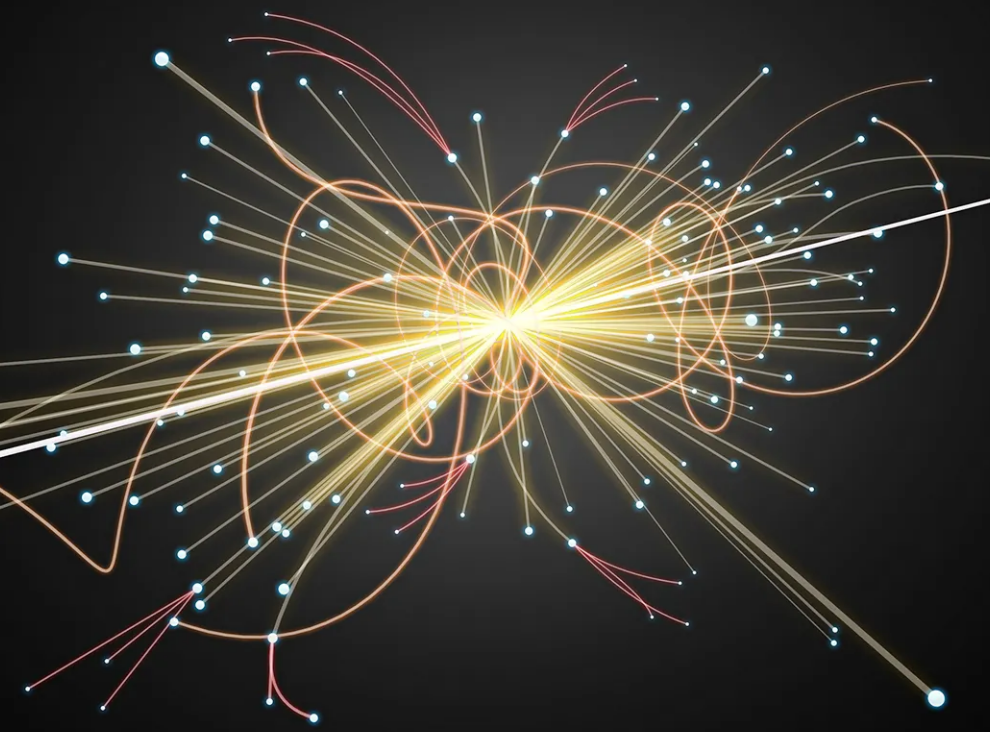
\includegraphics[width=0.90\textwidth]{graphics/lhc-particle-collision-523875355-f.png}
%\includegraphics[width=0.90\textwidth]{graphics/407533.jpg}
%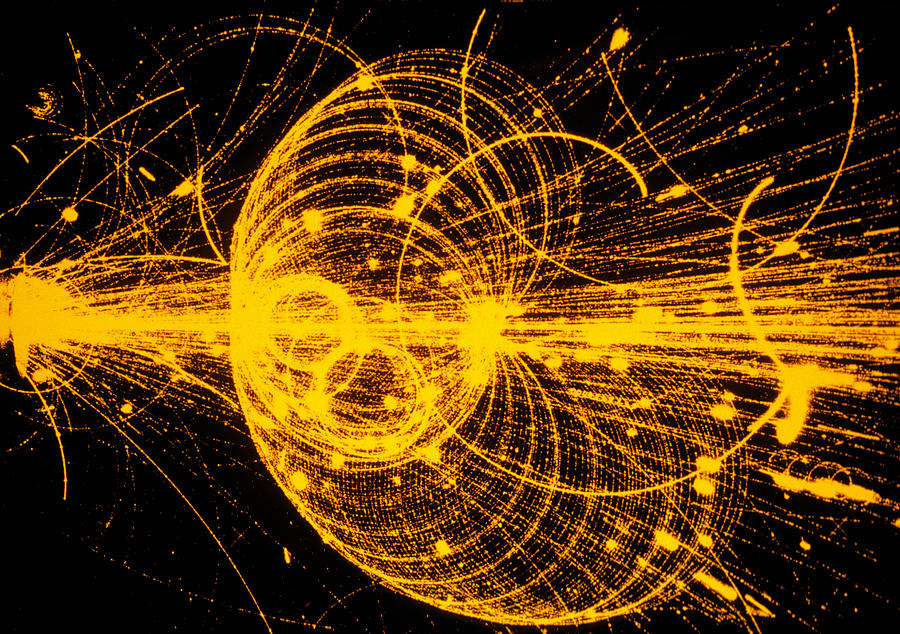
\includegraphics[width=0.95\textwidth]{graphics/streamer-chamber-photo-of-particle-tracks-cern.jpg}
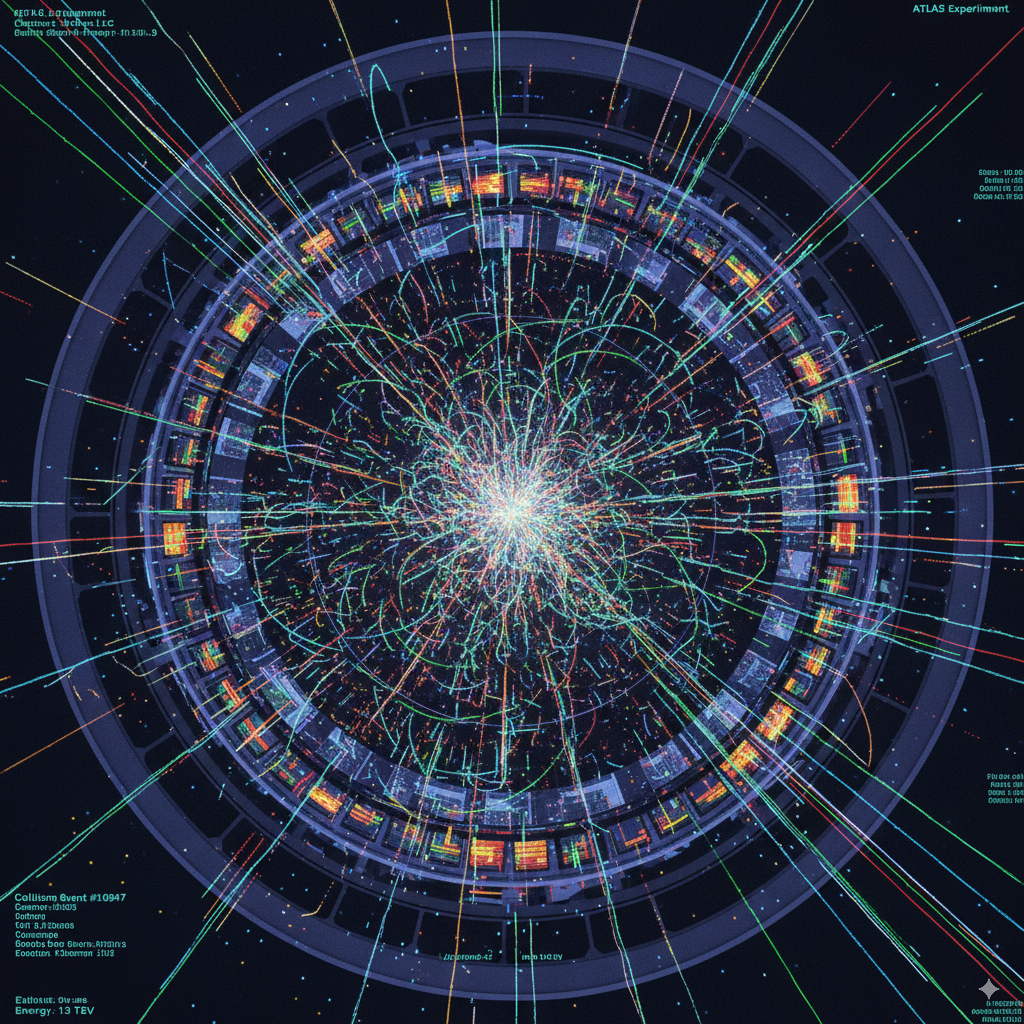
\includegraphics[width=0.75\textwidth]{graphics/Google-AIStudio-generated-particle-collision.png}
\vspace{0.1cm}

\LARGE
\textbf{\color{titlepagetext}\today}
            
\end{center}
\end{titlepage}

\pagecolor{white}

          %%%%% ~~~~~~~~~~~~~~~~~~~~ %%%%%

\pagestyle{fancy}

\lhead[Kenneth Chu]{Standard Model}
\rhead[Standard Model]{Kenneth Chu}
%\chead[]{{\Large\bf Mathematical Theory of the Standard Model of Particle Physics} \\ \vskip 0.1cm \normalsize \today}
\lfoot[]{}
\cfoot[]{}
\rfoot[]{\thepage}

          %%%%% ~~~~~~~~~~~~~~~~~~~~ %%%%%

\frontmatter
%\pagenumbering{roman}
%\setcounter{page}{1}
\tableofcontents

          %%%%% ~~~~~~~~~~~~~~~~~~~~ %%%%%

\mainmatter
%\pagenumbering{arabic}
%\setcounter{page}{0}

          %%%%% ~~~~~~~~~~~~~~~~~~~~ %%%%%

\chapter{Outline}
\setcounter{theorem}{0}
\setcounter{equation}{0}

%\cite{vanDerVaart1996}
%\cite{Kosorok2008}

%\renewcommand{\theenumi}{\alph{enumi}}
%\renewcommand{\labelenumi}{\textnormal{(\theenumi)}$\;\;$}
\renewcommand{\theenumi}{\roman{enumi}}
\renewcommand{\labelenumi}{\textnormal{(\theenumi)}$\;\;$}

          %%%%% ~~~~~~~~~~~~~~~~~~~~ %%%%%

\section{Key physical insight behind Standard Model: symmetries}

\begin{itemize}
\item
	\begin{equation*}
	\left.\begin{array}{c}
	\textnormal{Inadmissibility of \textit{action at a distance}}
	\\
	+
	\\
	\textnormal{States of a quantum system are to be}
	\\
	\textnormal{described by $1$-dimensional subspaces}
	\\
	\textnormal{in a complex Hilbert space}
	\end{array}\right\}
	\quad\Longrightarrow\quad
	\left\{\begin{array}{c}
	\textit{pre-quantized}
	\\
	\textnormal{descriptions of particles}
	\\
	\textnormal{will be sections of appropriate}
	\\
	\textnormal{complex vector bundles $E$}
	\end{array}\right.
	\end{equation*}
\item
	\underline{Principle of gauge invariance}
	\begin{equation*}
	\left.\begin{array}{c}
	\textnormal{Change of coordinatizaion}
	\\
	\textnormal{of internal spaces}
	\\
	\textnormal{should NOT change}
	\\
	\textnormal{physics}
	\end{array}\right\}
	\quad\Longrightarrow\quad
	\left\{\begin{array}{c}
	\textnormal{invariance of Lagrangian}
	\\
	\textnormal{under gauge transformations}
	\end{array}\right.
	\end{equation*}	
\item
	\underline{Symmetries exhibited by particles entail appearance of equivariant vector bundles}
	\begin{equation*}
	\left.\begin{array}{c}
	\textnormal{Particles exhibiting}
	\\
	\textnormal{internal symmetries}
	\end{array}\right\}
	\quad\Longrightarrow\quad
	\left\{\begin{array}{c}
	\textnormal{the complex vector bundle $E$}
	\\
	\textnormal{admits a $G$-action,}
	\\
	\textnormal{where $G$ is a compact Lie group}
	\\
	\textnormal{unrelated to spacetime symmetries}
	\end{array}\right.
	\end{equation*}
\item
	\underline{Symmetries exhibited by particles entail appearance of connections (gauge fields)}
	\begin{equation*}
	\left.\begin{array}{c}
	\textnormal{The Lagrangian density will involve}
	\\
	\textnormal{the fields themselves, as well as}
	\\
	\textnormal{the ``dynamics'' of the fields, i.e.,}
	\\
	\textnormal{first derivatives of the fields w.r.t. spacetime}
	\end{array}\right\}
	\quad\Longrightarrow\quad
	\left\{\begin{array}{c}
	\textnormal{Lagrangian will involve}
	\\
	\textnormal{\textit{connections} (``gauge fields'')}
	\\
	\textnormal{on the complex vector bundle $E$}
	\end{array}\right.
	\end{equation*}
	\textit{This is because complex vector bundles do NOT come canonically equipped with
	sufficient structure (i.e., connections) required for defining derivatives of its sections w.r.t. spacetime.}
\item
	\begin{equation*}
	%\left.
	\begin{array}{c}
	\textnormal{$G$-action on $E$}
	\end{array}
	%\right\}
	\quad\Longrightarrow\quad
	%\left\{
	\begin{array}{c}
	\textnormal{$G$-action on the connections (gauge fields) on $E$}
	\end{array}
	%\right.
	\end{equation*}
\item
	Suppose $E = P \times_{\rho}V$ is a complex vector bundle over a spacetime $\mathcal{M}$
	which is an associated vector bundle, where $P$ is a princpal $G$-bundle, and
	$\rho : G \longrightarrow \textnormal{GL}(V)$ is a representation.
	Then, is it true that every connection on $E$ is induced by a connection on $P$?
\end{itemize}

          %%%%% ~~~~~~~~~~~~~~~~~~~~ %%%%%

\section{Key physical insight behind Standard Model: Dirac's equation}
Dirac's equation seems to be the heart -- or key physical insight -- of the Standard Model (of particle physics),
in the sense that the rest of the Standard Model arguably follows from mathematics, or relatively straightforward
mathematical formulations of arguably self-evident physical constraints.
\begin{itemize}
\item
	Quantum mechanics was known to be insufficient -- there had been experimental observations
	that could not be explained with quantum mechanics.
	Quantum mechanics is incompatible with Special Relativity (e.g., there is an asymmetry between space and time
	in the Schr\"odinger equation).
	In particular, quantum mechanics fails to give accurate precisions for particles moving at speeds close to
	that of light.
\item
	\textbf{The Schr\"odinger equation:}
	\vskip 0.01cm
	According to Newtonian mechanics, the energy \,$E$\, and the momentum (vector) \,$\mathbf{p}$\,
	of a free particle (i.e., a particle on which no force is acting) of mass \,$m$\,
	satisfy the following identity:
	\begin{equation}
	\label{NewtonionEnergyMomemtumRelation}
	E \;=\; \dfrac{\Vert\,\mathbf{p}\,\Vert^{2}}{2m}
	\end{equation}
	The validity of this identity can be seen as follows:
	\begin{equation*}
	E
	\,:=\,
		\left(\!\begin{array}{c} \textnormal{total energy} \\ \textnormal{of the} \\ \textnormal{particle} \end{array}\!\right)
	\,=\,
		\left(\!\begin{array}{c} \textnormal{kinetic energy} \\ \textnormal{of the} \\ \textnormal{particle} \end{array}\!\right)
	\,=\,
		\dfrac{1}{2}\,m\,\Vert\,\mathbf{v}\,\Vert^{2}
	\,=\,
		\dfrac{(\,\Vert\,m\cdot\mathbf{v}\,\Vert\,)^{2}}{2m}
	\,=\,
		\dfrac{\Vert\,\mathbf{p}\,\Vert^{2}}{2m}\,,
	\end{equation*}
	where \,$\mathbf{v}$\, is the velocity vector of the particle.
	Writing
	\,$\mathbf{p} = (\,p_{1},p_{2},p_{3}\,)$,\,
	we may re-express
	\eqref{NewtonionEnergyMomemtumRelation}
	as follows:
	\begin{equation*}
	E \,-\, \dfrac{1}{2m}\left(\,p_{1}^{2} \overset{{\color{white}.}}{+} p_{2}^{2} + p_{3}^{2}\,\right) \;=\; 0
	\end{equation*}
	If we
	\begin{enumerate}
	\item
		replace -- according to canonical quantization -- the quantities
		\,$E$, $p_{1}$, $p_{2}$, $p_{3}$\,
		respectively with the following differential operations
		\begin{equation}
		\label{CanonicalQuantization}
		E \;\longmapsto\; \i\hbar\,\dfrac{\partial}{\partial t}\,,
		\quad\quad
		p_{j} \;\longmapsto\; -\,\i\hbar\,\dfrac{\partial}{\partial x_{j}}\,,
		\quad\quad
		\textnormal{and}
		\end{equation}
	\item
		let the resulting differential operator act on the wave function
		\,$\psi(t,x_{1},x_{2},x_{3})$\,,\,
	\end{enumerate}
	we arrive at the Schr\"odinger equation satisfied by the wave function
	\,$\psi(t,x_{1},x_{2},x_{3})$\,
	representing a free particle:
	\begin{equation*}
	\left(\,\i\hbar\,\dfrac{\partial}{\partial t} + \dfrac{\hbar^{2}}{2m}
		\left(
			\dfrac{\partial^{2}}{\partial x_{1}^{2}}
			+ \dfrac{\partial^{2}}{\partial x_{2}^{2}}
			+ \dfrac{\partial^{2}}{\partial x_{3}^{2}}
			\right)
		\,\right)
	\psi
	\,=\,
		0
	\end{equation*}
\item
	\textbf{The Klein-Gordon equation:}
	\vskip 0.01cm
	The asymmetry between time and space in the Schr\"odinger equation is obvious:
	the appearance of the first-order partial derivative with respect to time
	but second-order partial derivatives with respect to the spatial coordinates.
	One can also show that the Schr\"odinger equation is not Lorentz-invariant.
	It is thus clear that the Schr\"odinger equation is incompatible with special relativity.
	
	In order to remedy this, we derive a new quantum equation of motion by quantizing instead
	the relativistic counterpart of \eqref{NewtonionEnergyMomemtumRelation}:
	\begin{equation}
	\label{RelativisticEnergyMomemtumRelation}
	E^{2} \;=\; p^{2} \,+\, m^{2}
	\end{equation}
	Via the same quantization scheme
	\eqref{CanonicalQuantization}
	as before, we obtain the Klein-Gordon equation:
	\begin{equation*}
	\left(\,\dfrac{\partial^{2}}{\partial t^{2}}
	- \left(
		\dfrac{\partial^{2}}{\partial x_{1}^{2}}
		+ \dfrac{\partial^{2}}{\partial x_{2}^{2}}
		+ \dfrac{\partial^{2}}{\partial x_{3}^{2}}
		\right)
	\,+\,
		\dfrac{m^{2}}{\hbar^{2}}
		\,\right)
	\psi
	\,=\,
		0
	\end{equation*}
	The obvious asymmetry between space and time in the Schr\"odinger equation is no longer
	present in the Klein-Gordon equation.
	It is also straightforward to show that the Klein-Gordon equation is Lorentz-invariant.
	
	However, the Klein-Gordon equation is still theoretically unsatisfactory due to at least two facts:
	\begin{enumerate}
	\item[$\circ$]
		it is second-order in time, rendering it difficult to give it a dynamical interpretation, and
	\item[$\circ$]
		it allows negative-energy eigenstates.
	\end{enumerate}

\item
	\textbf{The Dirac equation:}
	\vskip 0.01cm
	Dirac sought a new equation of motion by seeking a first-order linear differential operator
	\begin{equation*}
	D
	\;=\;
		\gamma^{\mu}\partial_{\mu}
	\;=\;
		\gamma^{0}\dfrac{\partial}{\partial x_{0}} 
		\,+\, \gamma^{1}\dfrac{\partial}{\partial x_{1}} 
		\,+\, \gamma^{2}\dfrac{\partial}{\partial x_{2}} 
		\,+\, \gamma^{3}\dfrac{\partial}{\partial x_{3}} 
	\end{equation*}
	whose square is the d'Alembert operator
	\begin{equation*}
	\Box
	\;=\;
		\dfrac{\partial^{2}}{\partial t^{2}} \,-\, \Delta
	\;=\;
		\dfrac{\partial^{2}}{\partial t^{2}}
		\,-\, \dfrac{\partial^{2}}{\partial x_{1}^{2}}
		\,-\, \dfrac{\partial^{2}}{\partial x_{2}^{2}}
		\,-\, \dfrac{\partial^{2}}{\partial x_{3}^{2}}
	\end{equation*}
	in Minkowski spacetime. 
	Dirac arrived at the famous Dirac equation:
	\begin{equation*}
	\left(\,\i\cdot\gamma^{\mu}\partial_{\mu} - m\,\right)\psi \, = \, 0
	\end{equation*}
	A straightforward calculation shows that
	\,$\left(\,\i\cdot\gamma^{\mu}\partial_{\mu} - m\,\right)^{2} \,=\, \Box + m^{2}$\,
	if the ``coefficients'' \,$\gamma^{\mu}$\, satisfy:
	\begin{equation}
	\label{GammaMatricesSatisfyCliffordRelation}
	\left\{\,\gamma^{\mu}\,,\,\gamma^{\nu}\,\right\}
	\;=\;
		2\cdot g^{\mu\nu}\,,
	\end{equation}
	where
	\,$\left\{\,\gamma^{\mu}\,,\,\gamma^{\nu}\,\right\} \,:=\, \gamma^{\mu}\gamma^{\nu} + \gamma^{\mu}\gamma^{\nu}$\,
	and
	\,$g^{\mu\nu} \,=\, \diag(1,-1,-1,-1)$.\,

	Dirac realized that the condition \eqref{GammaMatricesSatisfyCliffordRelation} cannot be satisfied
	if the \,$\gamma^{\mu}$'s\, were just complex numbers, but that condition is indeed satisfied by
	certain $4 \times 4$ complex matrices.

	This observation led to the following realization (when expressed in modern geometric language):
	The ``wave function'' \,$\psi$\, must be smooth sections of a spinor bundle over spacetime.

\item
	\textbf{Relevance of spin structure: Each spinor bundle admits a unique Dirac operator}
	\vskip 0.01cm
	Recall that a spin structure on spacetime \,$M$\, 
	(pseudo-Riemannian 4-manifold with a Minkowski metric tensor)
	is a principal bundle 
	\,$\textnormal{Spin}(\Re^{1,3})  \hookrightarrow \widetilde{P} \longrightarrow M$\,
	over \,$M$\, which is a double cover of the orthonormal frame bundle of \,$M$:
	\begin{center}
	\begin{tikzcd}
	\textnormal{Spin}(\Re^{1,3})
		\arrow[rr]
		\arrow[dd, two heads, swap, "2:1\;"]
	&&
	\widetilde{P}
		\arrow[dd, two heads, "\;2:1"]
	\\ \\
	\mathcal{L}
		\arrow[rr]
	&&
	P
		\arrow[dd]
	\\ \\
	&&
	M
	\end{tikzcd}
	\end{center}
	where
	\begin{itemize}
	\item[$\circ$]
		$P \longrightarrow M$\, is the orthonormal frame bundle over \,$M$,\,
		which is a principal bundle whose structure group is the Lorentz group \,$\mathcal{L}$.\,
	\item[$\circ$]
		$\widetilde{P} \longrightarrow P$\, is the double covering,
	\item[$\circ$]
		$\textnormal{Spin}(\Re^{1,3}) \longrightarrow \mathcal{L}$\,
		is the universal (double) covering of the Lorentz group \,$\mathcal{L}$.
	\end{itemize}
	A spinor bundle is a complex vector bundle with fibre \,$\C^{2}$\, over spacetime \,$M$\, 
	associated to the principal bundle
	\,$\textnormal{Spin}(\Re^{1,3})  \hookrightarrow \widetilde{P} \longrightarrow M$\,
	via a representation:
	\begin{equation*}
	\rho \; : \; \textnormal{Spin}(\Re^{1,3}) \; \longrightarrow \textnormal{GL}(\C^{2})
	\end{equation*}
	The relevance of spin structures and spinor bundles is the following:
	\textbf{Each spinor bundle admits a unique Clifford connection, which in turn gives rise to a Dirac operator
	defined on that spinor bundle.
	In other words, smooth sections of spinor bundles are the entities for which the Dirac operator makes sense.}

\item
	The following considerations:
	\begin{itemize}
	\item[$\circ$]
		the local nature (no action at a distance) of a physical theory,
	\item[$\circ$]
		the fact that particles admit internal symmetries
	\end{itemize}
	together entails that the suitable mathematical objects to use to model
	internal symmetry varying over spacetime are:
	\begin{itemize}
	\item[$\circ$]
		principal fibre bundles
	\end{itemize}
	The (quantum mechanical) axiom that the states of a quantum system should be
	unit vectors in a given complex Hilbert space entails that the suitable mathematical
	objects to use to model particles are: smooth sections of complex vector bundles
	over spacetime associated to principal bundles whose structure groups induce
	(via group representations) the internal symmetries exhibited by the given quantum system.
\end{itemize}

          %%%%% ~~~~~~~~~~~~~~~~~~~~ %%%%%

\section{Outline -- older version}
\begin{itemize}
\item
	In the Standard Model of particle physics, ``particles'' are defined
	phenomenologically, in the sense that a ``particle'' is defined/identified/classified
	via its observed values of a number of characteristics,
	e.g. mass, charge, spin, colour, etc.
\item
	Each particle characteristic allow only a finite number of admissible values.
	These characteristics (hence the ``particles'' they phenomenologically define)
	are described mathematically as sections of certain vector bundles.
	
	Each admissible value of the characteristic corresponds
	to a $1$-dimensional subspace in the fibre.
	
	The laws of physics must be invariant under relabelling of the admissible values,
	which entails that the aforementioned vector bundles come with an action by a certain
	symmetry group $G$ that permutes the admissible values.
	In other words, these vector bundles are associated vector bundles of a
	principal fibre bundle with structure group $G$, induced by a certain representation
	of $G$ on the fibre space.
	
	These symmetries are called \textbf{gauge symmetries}.
\item
	The evolution in time of the ``particles'' is dictated by the curvature on the ambient vector bundle.
	In return, the presence of the particles affects the curvature on the ambient vector bundles.
	The dynamical interplay between the particle and curvature is determined by the principle
	of least action, i.e. the equation of motion is the Euler-Lagrange equations of a suitable
	action functional.
	
	The Lagrangian density (integrand of the action functional) must be
	Lorentz-invariant and gauge-invariant.
\item
	Creation and annihilation of particles are modelled by quantizing
	the Euler-Lagrange equations. 
\item
	Masses of fermions and the weak interaction bosons ($W^{\pm}$ and $Z^{0}$)
	are introduced by the Higgs mechanism.
	
	The non-zero ground state of the Higgs field ``breaks'' the fully gauge symmetry;
	after symmetry breaking, physics now ``happens'' on a sub-bundle of the original full bundle,
	with structure group $H \subset G$ being a subgroup of the original full unbroken gauge group $G$.
	Such an $H$ is the stabilizer subgroup of a certain vacuum element (a minimum of the Higgs potential)
	in the original fibre.
	
	``Mass'' terms for fermions and certain gauge bosons may appear
	when the original Lagrangian density is restricted to the reduced bundle,
	and re-expressed in terms intrinsic to the reduced bundle.
\end{itemize}

          %%%%% ~~~~~~~~~~~~~~~~~~~~ %%%%%



          %%%%% ~~~~~~~~~~~~~~~~~~~~ %%%%%

\chapter{Lagrangian mechanics}
\setcounter{theorem}{0}
\setcounter{equation}{0}

%\cite{vanDerVaart1996}
%\cite{Kosorok2008}

%\renewcommand{\theenumi}{\alph{enumi}}
%\renewcommand{\labelenumi}{\textnormal{(\theenumi)}$\;\;$}
\renewcommand{\theenumi}{\roman{enumi}}
\renewcommand{\labelenumi}{\textnormal{(\theenumi)}$\;\;$}

          %%%%% ~~~~~~~~~~~~~~~~~~~~ %%%%%

\begin{definition}[Lagrangian mechanical system, Definition 2.1, \cite{Cortes2017}]
\mbox{}
\vskip 0.1cm
\noindent
A \,\textbf{Lagrangian mechanical system}\, is a pair \,$\left(\,M,\mathscr{L}\,\right)$\,
consisting of a smooth manifold \,$M$ and a smooth $\Re$-valued function
\,$\mathscr{L} : TM \longrightarrow \Re$\,
defined on the tangent bundle \,$TM$ of \,$M$.
The manifold \,$M$ is called the \textbf{configuration space} and
the function \,$\mathscr{L}$\, is called the \textbf{Lagrangian function}
(or simply the \textbf{Lagrangian}) of the system.
\end{definition}

          %%%%% ~~~~~~~~~~~~~~~~~~~~ %%%%%

\vskip 0.5cm
\begin{definition}[Hamilton's principle of least action]
\mbox{}
\vskip 0.1cm
\noindent
Let \,$\left(\,M,\mathscr{L}\,\right)$ be a Lagrangian mechanical system.
The \,\textbf{action}\, of a smooth parametrized curve
\,$\gamma : [\,a, b\,] \longrightarrow M$\,
is defined as
\begin{equation*}
S(\,\gamma\,)
\;\; := \;\;
\int_{a}^{b}
\mathscr{L}(\,\gamma(t)\,)\,\d t.
\end{equation*}
A \,\textbf{motion}\, of the system is a critical point of \,$S$\,
under smooth variations with fixed endpoints.
(This statement is a mathematical formulation of
\textbf{Hamilton's principle of least action},
which should better be called principle of {\color{red}stationary} action.)
\end{definition}

          %%%%% ~~~~~~~~~~~~~~~~~~~~ %%%%%

\vskip 0.5cm
\begin{definition}[Induced coordinate systems]
\mbox{}
\vskip 0.1cm
\noindent
Suppose:
\begin{itemize}
\item
	$\left(\,M,\mathscr{L}\,\right)$ is a Lagrangian mechanical system, with \,$n \,:=\, \dim(M)$, and
\item
	$(x^{1},\ldots,x^{n}) : U \subset M \longrightarrow \Re^{n}$\,
	is a local coordinate system.
\end{itemize}
Then, the \,\textbf{induced coordinate sytem}\, of \,$(x^{1},\ldots,x^{n})$\, is
\,$\left(\,q^{1},\ldots,q^{n},\hat{q}^{\,1},\ldots,\hat{q}^{\,n}\,\right) : \pi^{-1}(U) \longrightarrow \Re^{2n}$\,
given by
\begin{equation*} 
q^{i} \; := \; x^{i} \circ \pi \,:\, \pi^{-1}(U) \,\longrightarrow\, \Re,
\quad\textnormal{and}\quad
\hat{q}^{\,i} \; := \; \d x^{i} \,:\, \pi^{-1}(U) \,\longrightarrow\, \Re\,,
\end{equation*}
where \,$\pi : TM \longrightarrow M$\, is the canoncial projection.
\end{definition}

          %%%%% ~~~~~~~~~~~~~~~~~~~~ %%%%%

\vskip 0.5cm
\begin{remark}[Gradient of the Lagrangian function w.r.t. an induced coordinate system]
\mbox{}
\vskip 0.1cm
\noindent
Note that
\begin{equation*}
\nabla_{(q^{1},\ldots,q^{n},\hat{q}^{\,1},\ldots,\hat{q}^{\,n})}\,\mathscr{L}
\;\; = \;\;
	\left(\,
		\dfrac{\partial\mathscr{L}}{\partial q^{1}}\,,
		\,\ldots\,,
		\dfrac{\partial\mathscr{L}}{\partial q^{n}}\,,
		\dfrac{\partial\mathscr{L}}{\partial \hat{q}^{\,1}}\,,
		\,\ldots\,
		\dfrac{\partial\mathscr{L}}{\partial \hat{q}^{\,n}}
		\,\right)
\; : \;
	\pi^{-1}(U) \; \longrightarrow \; \Re^{2n}
\end{equation*}
The component functions of
\,$\nabla_{(q^{1},\ldots,q^{n},\hat{q}^{\,1},\ldots,\hat{q}^{\,n})}\,\mathscr{L}$\,
appear in the Euler-Lagrange equations,
the ordinary differential equations that determine the motions
of a Lagrangian mechanical system;
see Proposition \ref{EulerLagrangeEquations}.
\end{remark}

          %%%%% ~~~~~~~~~~~~~~~~~~~~ %%%%%

\vskip 0.5cm
\begin{proposition}[Equations of motion, Euler-Lagrangian equations]
\label{EulerLagrangeEquations}
\mbox{}
\vskip 0.1cm
\noindent
A smooth parametrized curve
\,$\gamma : [\,a,b\,] \longrightarrow M$\,
in a Lagrangian mechanical system
\,$\left(\,M,\mathscr{L}\,\right)$\,
is a motion if and only if
\,$\gamma$\,
satisfies the following ordinary differential equations:
\begin{equation*}
\dfrac{\partial\mathscr{L}}{\partial q^{i}}\!\left(\gamma^{\prime}(t)\right)
\; - \;
\dfrac{\d}{\d t}\!\left(\,\dfrac{\partial\mathscr{L}}{\partial \hat{q}^{\,i}}\!\left(\gamma^{\prime}(t)\right)\right)
\;\; = \;\;
0\,,
\end{equation*}
for each \,$i = 1, 2, \,\ldots\, , n \,:=\, \dim(M)$,
each \,$t \in [\,a,b\,]$, and
each induced coordinate system\\
\,$\left(\,q^{1},\ldots,q^{n},\hat{q}^{\,1},\ldots,\hat{q}^{\,n}\,\right)$\,
containing \,$\gamma(t) \in M$.
\end{proposition}
\proof
\begin{equation}\label{VariationVectorField}
\left.\dfrac{\d}{\d s}\right\vert_{s=0} \mathscr{L}\!\left(\gamma_{s}(t)\right)
\;\; = \;\;
	\overset{n}{\underset{i=1}{\sum}}\,\left\{\,
		\dfrac{\partial\mathscr{L}}{\partial q^{i}}\!\left(\gamma^{\prime}_{0}(t)\right)
		\cdot
		\left.\dfrac{\d}{\d s}\right\vert_{s=0} q^{i}(\gamma^{\prime}_{s}(t))
		\, + \,
		\dfrac{\partial\mathscr{L}}{\partial\hat{q}^{\,i}}\!\left(\gamma^{\prime}_{0}(t)\right)
		\cdot
		\left.\dfrac{\d}{\d s}\right\vert_{s=0} \hat{q}^{\,i}(\gamma^{\prime}_{s}(t))
		\,\right\}
\end{equation}
Now, observe that
\begin{eqnarray*}
\left.\dfrac{\d}{\d s}\right\vert_{s=0} \hat{q}^{\,i}(\gamma^{\prime}_{s}(t))
& = &
	\left.\dfrac{\d}{\d s}\right\vert_{s=0} \d x^{i}(\gamma^{\prime}_{s}(t))
\;\; = \;\;
	\left.\dfrac{\d}{\d s}\right\vert_{s=0} \, \dfrac{\d}{\d t}\,(x^{i}\circ\gamma_{s})(t)
\;\; = \;\;
	\dfrac{\d}{\d t}\; \left.\dfrac{\d}{\d s}\right\vert_{s=0} \, (x^{i}\circ\gamma_{s})(t)
\\
& = &
	\overset{{\color{white}1}}{\dfrac{\d}{\d t}}\, W^{i}(t),
\end{eqnarray*}
where
\,$W(t) \,:=\, \left.\dfrac{\d}{\d s}\right\vert_{s=0} \gamma_{s}(t) \,\in\, T_{\gamma(t)}M$\,
is the variation vector field defined along \,$\gamma$.
Hence,
\begin{eqnarray*}
\dfrac{\partial\mathscr{L}}{\partial\hat{q}^{\,i}}\!\left(\gamma^{\prime}_{0}(t)\right)
\cdot
\left.\dfrac{\d}{\d s}\right\vert_{s=0} \hat{q}^{\,i}(\gamma^{\prime}_{s}(t))
& = &
	\dfrac{\partial\mathscr{L}}{\partial\hat{q}^{\,i}}\!\left(\gamma^{\prime}_{0}(t)\right)
	\cdot
	\dfrac{\d}{\d t}\, W^{i}(t)	
\\
& = &
	\dfrac{\d}{\d t}\!\left(\,
		\dfrac{\partial\mathscr{L}}{\partial\hat{q}^{\,i}}\!\left(\gamma^{\prime}_{0}(t)\right)
		\cdot
		W^{i}(t)
		\right)
	\, - \,
	\dfrac{\d}{\d t}\!\left(\,
		\dfrac{\partial\mathscr{L}}{\partial\hat{q}^{\,i}}\!\left(\gamma^{\prime}_{0}(t)\right)
		\right)	
	\cdot
	W^{i}(t)
\end{eqnarray*}
Substituting the above into \eqref{VariationVectorField} yields:
\begin{eqnarray*}
&&
	\left.\dfrac{\d}{\d s}\right\vert_{s=0} \mathscr{L}\!\left(\gamma_{s}(t)\right)
\\
& = &
	\overset{n}{\underset{i=1}{\sum}}\,\left\{\,
		\dfrac{\partial\mathscr{L}}{\partial q^{i}}\!\left(\gamma^{\prime}_{0}(t)\right)
		\cdot
		\left.\dfrac{\d}{\d s}\right\vert_{s=0} q^{i}(\gamma^{\prime}_{s}(t))
		\, + \,
		\dfrac{\partial\mathscr{L}}{\partial\hat{q}^{\,i}}\!\left(\gamma^{\prime}_{0}(t)\right)
		\cdot
		\left.\dfrac{\d}{\d s}\right\vert_{s=0} \hat{q}^{\,i}(\gamma^{\prime}_{s}(t))
		\,\right\}
\\
& = &
	\overset{n}{\underset{i=1}{\sum}}\,\left\{\,
		\dfrac{\partial\mathscr{L}}{\partial q^{i}}\!\left(\gamma^{\prime}(t)\right)
		\cdot
		\left.\dfrac{\d}{\d s}\right\vert_{s=0} x^{i}\circ\pi(\gamma^{\prime}_{s}(t))
		\, - \,
		\dfrac{\d}{\d t}\!\left(\,
			\dfrac{\partial\mathscr{L}}{\partial\hat{q}^{\,i}}\!\left(\gamma^{\prime}(t)\right)
			\right)	
		\cdot
		W^{i}(t)
		\,\right\}
	\; + \;
	\dfrac{\d}{\d t}\!\left(\,
		\overset{n}{\underset{i=1}{\sum}}\;
		\dfrac{\partial\mathscr{L}}{\partial\hat{q}^{\,i}}\!\left(\gamma^{\prime}(t)\right)
		\cdot
		W^{i}(t)
		\right)
\\
& = &
	\overset{n}{\underset{i=1}{\sum}}\,\left\{\,
		\dfrac{\partial\mathscr{L}}{\partial q^{i}}\!\left(\gamma^{\prime}(t)\right)
		\cdot
		\left.\dfrac{\d}{\d s}\right\vert_{s=0} x^{i}\circ\gamma_{s}(t)
		\, - \,
		\dfrac{\d}{\d t}\!\left(\,
			\dfrac{\partial\mathscr{L}}{\partial\hat{q}^{\,i}}\!\left(\gamma^{\prime}(t)\right)
			\right)	
		\cdot
		W^{i}(t)
		\,\right\}
	\; + \;
	f^{\prime}(t)
\\
& = &
	\overset{n}{\underset{i=1}{\sum}}\,\left\{\;
		\dfrac{\partial\mathscr{L}}{\partial q^{i}}\!\left(\gamma^{\prime}(t)\right)
		\, - \,
		\dfrac{\d}{\d t}\!\left(\,
			\dfrac{\partial\mathscr{L}}{\partial\hat{q}^{\,i}}\!\left(\gamma^{\prime}(t)\right)
			\right)
		\right\}
	\cdot
	W^{i}(t)
	\; + \;
	f^{\prime}(t)
\end{eqnarray*}
where
\begin{equation*}
f(t)
\;\; := \;\;
	\overset{n}{\underset{i=1}{\sum}}\;
	\dfrac{\partial\mathscr{L}}{\partial\hat{q}^{\,i}}\!\left(\gamma^{\prime}(t)\right)
	\cdot
	W^{i}(t)\,,
\quad
\textnormal{for \,$t \in [\,a,b\,]$}
\end{equation*}

\vskip 0.5cm
\noindent
\textbf{Claim 1:}
\vskip 0.1cm
\noindent
$f : [\,a,b\,] \longrightarrow \Re$\, is globally well-defined on \,$[\,a,b\,]$;\,
more precisely, the local definition of \,$f$\, above is in fact
independent of the choice of the local coordinate system.
Furthermore, \,$f(a) = f(b) = 0$.
\vskip 0.2cm
\noindent
Proof of Claim 1: \quad
\begin{equation*}
T^{\textnormal{ver}}_{\gamma(t)}(TM)
\;\; := \;\;
	\textnormal{ker}\!\left(\,\d\pi\vert_{\gamma(t)}\,\right)
\;\; \subset \;\;
	T_{\gamma(t)}(TM).
\end{equation*}
\begin{eqnarray*}
&&
	\left.\dfrac{\d}{\d s}\right\vert_{s=0} S\!\left(\gamma_{s}\right)
\\
& = &
	\left.\dfrac{\d}{\d s}\right\vert_{s=0}\; \int_{a}^{b}\,\mathscr{L}\!\left(\gamma_{s}(t)\right)\d t
\;\; = \;\;
	\int_{a}^{b}\left(\left.\dfrac{\d}{\d s}\right\vert_{s=0}\,\mathscr{L}\!\left(\gamma_{s}(t)\right)\right)\d t
\\
& = &
	\int_{a}^{b}\left(\;
		\overset{n}{\underset{i=1}{\sum}}\,\left\{\;
			\dfrac{\partial\mathscr{L}}{\partial q^{i}}\!\left(\gamma^{\prime}(t)\right)
			\, - \,
			\dfrac{\d}{\d t}\!\left(\,
				\dfrac{\partial\mathscr{L}}{\partial\hat{q}^{\,i}}\!\left(\gamma^{\prime}(t)\right)
				\right)
			\right\}
		\cdot
		W^{i}(t)
		\; + \;
		f^{\prime}(t)
		\right)\d t
\\
& = &
	\int_{a}^{b}\left(\;
		\overset{n}{\underset{i=1}{\sum}}\,\left\{\;
			\dfrac{\partial\mathscr{L}}{\partial q^{i}}\!\left(\gamma^{\prime}(t)\right)
			\, - \,
			\dfrac{\d}{\d t}\!\left(\,
				\dfrac{\partial\mathscr{L}}{\partial\hat{q}^{\,i}}\!\left(\gamma^{\prime}(t)\right)
				\right)
			\right\}
		\cdot
		W^{i}(t)
		\right)\d t
	\; + \;
	\left(\, f(b) \overset{{\color{white}1}}{-} f(a) \,\right)
\\
& = &
	\int_{a}^{b}\left(\;
		\overset{n}{\underset{i=1}{\sum}}\,\left\{\;
			\dfrac{\partial\mathscr{L}}{\partial q^{i}}\!\left(\gamma^{\prime}(t)\right)
			\, - \,
			\dfrac{\d}{\d t}\!\left(\,
				\dfrac{\partial\mathscr{L}}{\partial\hat{q}^{\,i}}\!\left(\gamma^{\prime}(t)\right)
				\right)
			\right\}
		\cdot
		W^{i}(t)
		\right)\d t
\end{eqnarray*}

\qed

          %%%%% ~~~~~~~~~~~~~~~~~~~~ %%%%%

          %%%%% ~~~~~~~~~~~~~~~~~~~~ %%%%%

          %%%%% ~~~~~~~~~~~~~~~~~~~~ %%%%%



          %%%%% ~~~~~~~~~~~~~~~~~~~~ %%%%%

\chapter{Symplectic geometry}
\setcounter{theorem}{0}
\setcounter{equation}{0}

%\cite{vanDerVaart1996}
%\cite{Kosorok2008}

%\renewcommand{\theenumi}{\alph{enumi}}
%\renewcommand{\labelenumi}{\textnormal{(\theenumi)}$\;\;$}
\renewcommand{\theenumi}{\roman{enumi}}
\renewcommand{\labelenumi}{\textnormal{(\theenumi)}$\;\;$}

          %%%%% ~~~~~~~~~~~~~~~~~~~~ %%%%%

\begin{theorem}
\mbox{}
\vskip 0.2cm
\noindent
Suppose $(M,\omega)$ is symplectic manifold. Then,
\begin{enumerate}
\item
	The set $C^{\infty}(M)$ of smooth $\Re$-valued functions on $M$
	forms a Lie algebra under the Poisson bracket.
\item
	The set $V^{\textnormal{LH}}(M)$ of locally Hamiltonian vector fields defined on $M$
	forms a Lie algebra under the Lie bracket, and
	the set $V^{\textnormal{H}}(M) \subset V^{\textnormal{LH}}(M)$ of (globally) Hamiltonian vector fields
	is a Lie algebra ideal of $V^{\textnormal{LH}}(M)$.
\item
	For each $f \in C^{\infty}(M)$, let $X_{f} \in V^{\textnormal{H}}(M)$ denotes the Hamiltonian vector field generated by $f$.
	Then, the map $C^{\infty}(M) \longrightarrow V^{\textnormal{H}}(M)$ is a Lie algebra homomorphism
	with kernel being the set of constant $\Re$-valued functions on $M$.
	In particular, we have the following Lie-algebra isomorphism
	\begin{equation*}
	V^{\textnormal{H}}(M) \;\; \cong \;\; C^{\infty}(M) \,/\, \Re.
	\end{equation*}
\end{enumerate}
\end{theorem}

          %%%%% ~~~~~~~~~~~~~~~~~~~~ %%%%%

          %%%%% ~~~~~~~~~~~~~~~~~~~~ %%%%%



          %%%%% ~~~~~~~~~~~~~~~~~~~~ %%%%%

\chapter{Time-dependent perturbation theory and the interaction picture}
\setcounter{theorem}{0}
\setcounter{equation}{0}

%\cite{vanDerVaart1996}
%\cite{Kosorok2008}

%\renewcommand{\theenumi}{\alph{enumi}}
%\renewcommand{\labelenumi}{\textnormal{(\theenumi)}$\;\;$}
\renewcommand{\theenumi}{\roman{enumi}}
\renewcommand{\labelenumi}{\textnormal{(\theenumi)}$\;\;$}

          %%%%% ~~~~~~~~~~~~~~~~~~~~ %%%%%

We want to determine the time-evolution of a system under the time-varying Hamiltonian
\begin{equation*}
H(t) \;\; = \;\; H_{0} \,+\, H_{1}(t)
\end{equation*}

\vskip 0.5cm
\noindent
\textbf{Comments}
\begin{itemize}
\item
	We seek solution in the form of a one-parameter family of unitary operators
	\,$U(t)$\, which satisfies
	\begin{equation*}
	\dfrac{\d}{\d t}\,U(t) \;\; = \;\; -\,\i\,H(t)\,U(t)\,,
	\quad
	\textnormal{where \,$\i \,:=\, \sqrt{-1}$}
	\end{equation*}
\item
	We assume we know that the time-evolution of a system under the constant (with respect to time)
	Hamiltonian $H_{0}$ is given by
	\begin{equation*}
	U_{0}(t) \;\; = \;\; \exp\left(\,-\,\i\,t\,H_{0}\,\right),
	\end{equation*}
	which is determined as the solution of:
	\begin{equation*}
	\left\{\;\;
		\begin{array}{ccc}
		\dfrac{\d}{\d t}\,U_{0}(t) & = & -\,\i\,H_{0}\,U_{0}(t)
		\\
		\overset{{\color{white}1}}{U_{0}(0)} & = & \textnormal{identity operator}
		\end{array}
		\right.
	\end{equation*}
\end{itemize}

          %%%%% ~~~~~~~~~~~~~~~~~~~~ %%%%%

\vskip 0.5cm
\section{The interaction picture}

The situation where we time-evolve the operator \,$A$\, according to
\begin{equation*}
A(t) \;\; = \;\; U_{0}(-t) \cdot A \cdot U_{0}(t)
\end{equation*}
and the state \,$x(t)$\, according to
\begin{equation*}
x(t) \;\; = \;\; U_{0}(-t) \cdot U(t) \cdot x
\end{equation*}
is called the \textbf{interaction picture}.
Note that the interaction picture is consistent with both the Schr\"odinger and the Heisenberg pictures:
\begin{eqnarray*}
\left\langle\; \overset{{\color{white}.}}{x(t)} \,,\, A(t) \cdot x(t) \;\right\rangle
& = &
	\left\langle\;
		\overset{{\color{white}.}}{U_{0}(-t)} \cdot U(t) \cdot x
		\;\,,\;
		U_{0}(-t) \cdot A \cdot U_{0}(t) \cdot U_{0}(-t) \cdot U(t) \cdot x
		\;\right\rangle
\\
& = &
	\left\langle\;
		\overset{{\color{white}.}}{U(t)} \cdot x
		\;\,,\;
		A \cdot U(t) \cdot x
		\;\right\rangle
	\quad\quad
	\textnormal{(Schr\"odinger picture)}
\\
& = &
	\left\langle\;
		\overset{{\color{white}.}}{U(-t)} \cdot U(t) \cdot x
		\;\,,\;
		U(-t) \cdot A \cdot U(t) \cdot x
		\;\right\rangle
\\
& = &
	\left\langle\;
		x
		\;\,,\;
		\overset{{\color{white}.}}{U(-t)} \cdot A \cdot U(t) \cdot x
		\;\right\rangle
	\quad\quad
	\textnormal{(Heisenberg picture)}
\end{eqnarray*}

          %%%%% ~~~~~~~~~~~~~~~~~~~~ %%%%%

\vskip 0.5cm
\section{The Dyson expansion}
\begin{proposition}[Dyson expansion]
\mbox{}\vskip 0.2cm
\noindent
Define \,$V(t) \, := \, U_{0}(t)^{-1} \cdot U(t) \, = \, U_{0}(-t) \cdot U(t)$.\,
Then, the following statements are true:
\begin{enumerate}
\item
	We have:\quad $U(t) \,= \, U_{0}(t) \cdot V(t)$
\item
	$V(t)$\, satisfies:
	\begin{equation*}
	\dfrac{\d}{\d t}\,V(t) \;\; = \;\; -\,\i\,\widetilde{H}_{1}(t)\,V(t)\,,
	\end{equation*}	
	where
	\begin{equation*}
	\widetilde{H}_{1}(t) \;\; := \;\; U_{0}(-t) \cdot H_{1}(t) \cdot U_{0}(t)
	\end{equation*}	
\item
	$V(t)$ can be expressed as:
	\begin{equation*}
	V(t) \;\; = \;\; \mathbf{1} \, + \, \overset{\infty}{\underset{n = 1}{\sum}}\,W_{n}(t)\,,
	\end{equation*}
	where
	\begin{equation*}
	W_{n}(t) \;\; = \;\; (-\i)^{n}\cdot
		\int_{0}^{t}\d\theta_{1} \, \int_{0}^{\theta_{1}}\d\theta_{2} \;\, \cdots \,  \int_{0}^{\theta_{n-1}}\d\theta_{n}
			\left(\,
				\overset{{\color{white}1}}{\widetilde{H}_{1}(\theta_{1})}
				\cdot
				\widetilde{H}_{1}(\theta_{2})
				\,\cdots\,
				\widetilde{H}_{1}(\theta_{n})
				\,\right),
	\;\;
	\end{equation*}
	for \,$n = 1, 2, \ldots$
\item
	For \,$n = 1, 2, \ldots$\,, \,$W_{n}(t)$\, can be expressed as:
	\begin{equation*}
	W_{n}(t) \;\; = \;\; \dfrac{(-\i)^{n}}{n!}\cdot
		\int_{0}^{t}\d\theta_{1} \, \int_{0}^{t}\d\theta_{2} \;\, \cdots \,  \int_{0}^{t}\d\theta_{n}\;
			\mathcal{T}\!\left(\,
				\overset{{\color{white}1}}{\widetilde{H}_{1}(\theta_{1})}
				\cdot
				\widetilde{H}_{1}(\theta_{2})
				\,\cdots\,
				\widetilde{H}_{1}(\theta_{n})
				\,\right),
	\end{equation*}
	where \,$\mathcal{T}(\,\cdot\,)$ is the \textbf{chronological operator}, defined as follows:
	\begin{equation*}
	\mathcal{T}\!\left(\,
		\overset{{\color{white}1}}{\widetilde{H}_{1}(\theta_{1})}
		\cdot
		\widetilde{H}_{1}(\theta_{2})
		\,\cdots\,
		\widetilde{H}_{1}(\theta_{n})
		\,\right)
	\;\; := \;\;
		\overset{{\color{white}1}}{\widetilde{H}_{1}(\theta_{\sigma(1)})}
		\cdot
		\widetilde{H}_{1}(\theta_{\sigma(2)})
		\,\cdots\,
		\widetilde{H}_{1}(\theta_{\sigma(n)})\,,
	\end{equation*}
	where \,$\sigma \in S_{n}$\, is any permutation of $\{1,2,\cdots,n\}$ such that
	\begin{equation*}
	\theta_{\sigma(1)} \; \leq \; \theta_{\sigma(2)} \; \leq \; \cdots \; \leq \; \theta_{\sigma(n)}
	\end{equation*}
\item
	For \,$H_{1}(t) \,=\, \kappa\,H_{I}$,\,
	\begin{equation*}
	V(t) \;\; = \;\; \mathbf{1} \, + \,
		\overset{\infty}{\underset{n = 1}{\sum}}\, \dfrac{(-\i\,\kappa)^{n}}{n!}
		\cdot
		\int_{0}^{t}\d\theta_{1} \, \int_{0}^{t}\d\theta_{2} \;\, \cdots \,  \int_{0}^{t}\d\theta_{n}\;
			\mathcal{T}\!\left(\,
				\overset{{\color{white}1}}{H_{I}(\theta_{1})}
				\cdot
				H_{I}(\theta_{2})
				\,\cdots\,
				H_{I}(\theta_{n})
				\,\right),
	\end{equation*}
	where \,$H_{I}(t) \, := \, U_{0}(-t) \cdot H_{I} \cdot U_{0}(t)$.
\end{enumerate}
\end{proposition}


          %%%%% ~~~~~~~~~~~~~~~~~~~~ %%%%%



          %%%%% ~~~~~~~~~~~~~~~~~~~~ %%%%%

\clearpage
\appendix

          %%%%% ~~~~~~~~~~~~~~~~~~~~ %%%%%

\chapter{The structure of a quantum field theory}
\setcounter{theorem}{0}
\setcounter{equation}{0}

%\cite{vanDerVaart1996}
%\cite{Kosorok2008}

%\renewcommand{\theenumi}{\alph{enumi}}
%\renewcommand{\labelenumi}{\textnormal{(\theenumi)}$\;\;$}
\renewcommand{\theenumi}{\roman{enumi}}
\renewcommand{\labelenumi}{\textnormal{(\theenumi)}$\;\;$}

          %%%%% ~~~~~~~~~~~~~~~~~~~~ %%%%%

A quantum field theory is a modification of quantum mechanics
so that the resulting theory becomes compatible with special relativity,
at least in the following sense:
\begin{itemize}
\item
	space and time must be treated on equal footing in a quantum field theory, and
\item
	a quantum field theory must be able to describe (highly energetic)
	interactions of (initial) particles where
	\begin{itemize}
	\item
		the final (i.e., post-interaction) number of particles is different
		from the initial (i.e., pre-interaction) number of particles, and
	\item
		the species of the post-interaction particles are different
		from those of the pre-interaction particles.
	\end{itemize}
	This is because, according to special relativity, energy and mass are exchangeable;
	hence, sufficiently (highly) energetic particle interactions are capable of converting
	the mass and energy of the pre-interaction particles into a collection of post-interaction
	particles that has a different number of particles and are of different species as the pre-interaction particles.
\end{itemize}

          %%%%% ~~~~~~~~~~~~~~~~~~~~ %%%%%

\noindent
In a quantum field theory:
\begin{itemize}
\item
	Recall that, in quantum mechanics, the states of a particle are represented by one-dimensional subspaces
	in a complex Hilbert space $\mathcal{H}$.
	\vskip 0.1cm
	Recall that the Poincaré group is the symmetry group of spacetime in special relativity.
	One thus expects that the Poincaré group to admit a unitary action on $\mathcal{H}$.
	\vskip 0.1cm
	We assume that the particle is ``elementary'' (i.e., is not the bound state of more elementary constituent particles)
	if and only if its corresponding Poincaré group (unitary) action on $\mathcal{H}$ is irreducible.
\item
	Since elementary particles exhibit ``internal symmetry'', we also expect that,
	for each species of elementary particles and
	for each internal symmetry exhibited by this given species of elementary particles,
	there corresponds an irreducible unitary representation of the internal symmetry group
	on some finite-dimensional complex Hilbert space.
	The finite-dimensionality assumption here is due to the belief (and experimental observations)
	that the number of possible states ``generated'' under each such internal symmetry group action is finite.
\item
	In order to avoid ``action at a distance'', one therefore expects that each (non-interacting) species
	of elementary particles to be mathematically describable -- in ``pre-quantized'' form -- by a section of a complex vector bundle
	over spacetime (position Minkowski space), equipped with a Poincaré group action
	as well as (fibrewise) actions of internal symmetry groups.
	The fibre of this complex vector bundle will be the tensor product of $L^{2}(\Re^{1,3},\d\mu)$
	with the state spaces (which are finite-dimensional complex Hilbert spaces) of the internal symmetry groups
	of the given elementary particle species.
	\vskip 0.1cm
	One such appropriate class of complex vector bundles is the vector bundles associated with principle fibre bundles.	
\item
	Since physical phenomena should be unaffected by the aforementioned
	vector bundles and principal fibre bundles are ``coordinatized'', one expects that
	any physical law to be Poincaré-invariant as well as gauge invariant (i.e., invariant under the internal symmetry actions). 
\item
	Poincaré-invariant and gauge-invariant Lagrangian density: $\mathcal{L}(\,\cdots\,)$.
	From classical mechanics, one expects the Lagrangian to involve the field $\phi$ as well as its first derivatives:
	\begin{equation*}
	\mathcal{L} \;\; = \;\; \mathcal{L}(\phi,\partial\phi),
	\end{equation*}
	where the occurrence of the first derivative $\partial\phi$ of the field $\phi$ is expected to be related to dynamics.
	\vskip 0.1cm
	However, on an associated vector bundle of a principal fibre bundle, there is in fact no canonically defined notion
	of derivatives (of sections of the vector bundle).
	We need the extra structure of a \textit{connection} $A$ on the principal fibre bundle
	in order to be able to define the (covariant) derivative $D_{A}(\,\phi\,)$ of $\phi$ with respect to $A$.
	Thus, we expect the Lagrangian to be of the following form instead:
	\begin{equation*}
	\mathcal{L} \;\; = \;\; \mathcal{L}\!\left(\,\overset{{\color{white}.}}{\phi}\,,D_{A}(\,\phi\,)\right).
	\end{equation*}
\item
	The Lagrangian density will be of the form:
	\begin{equation*}
	\mathcal{L}
	\;\; = \;\;
		\mathcal{L}_{\textnormal{\,free}}\!\left(\,\overset{{\color{white}.}}{\phi}\,,D_{A}(\,\phi\,)\right)
	\,+\,
		\mathcal{L}_{\textnormal{\,int}}\!\left(\,\overset{{\color{white}.}}{\phi}\,,D_{A}(\,\phi\,)\right)
	\end{equation*}
	\begin{itemize}
	\item
		The ``free'' part $\mathcal{L}_{\textnormal{\,free}}\!\left(\,\overset{{\color{white}.}}{\phi}\,,D_{A}(\,\phi\,)\right)$
		describes non-interacting particles.
	\item
		In order to use perturbative methods, the full Lagrangian
		$\mathcal{L} = \mathcal{L}_{\textnormal{\,free}} + \mathcal{L}_{\textnormal{\,int}}$
		needs to be a small perturbation of $\mathcal{L}_{\textnormal{\,free}}$.
	\item
		Usually, one derives/guesses the relativistic wave equation satisfied by a
		non-interacting field $\phi_{\,\textnormal{free}}(x)$.
		Then, the free part $\mathcal{L}_{\textnormal{\,free}}$ can be reverse-engineered
		from the relativistic wave equation, knowing the latter is the Euler-Lagrange equation
		of the former ($\mathcal{L}_{\textnormal{\,free}}$).
	\item
		The relativistic wave equation will turn out to be second-order partial differential equations
		with constant coefficients, and can be solved using Fourier transforms as integrals over
		momentum Minkowski space of scalar multiples of plane wave solutions
		(indexed by momentum $4$-vector).
		The coefficients $a(p)$ and $a^{\dagger}(p)$
		of the plane wave solutions $\exp(-\,\sqrt{-1}\cdot xp)$ and $\exp(+\,\sqrt{-1}\cdot xp)$
		in the integrand are thus functions defined momentum $4$-space.
	\item
		The notion/procedure of \textit{second quantization} involves ``re-interpreting''
		$\phi_{\,\textnormal{free}}(x)$ as operators on a suitable complex Hilbert space (Fock space)
		satisfying certain commutation relations.
		These commutation relations (satisfied by $\phi_{\,\textnormal{free}}$) will in turn imply that
		the resulting operators corresponding to $a(p)$ and $a^{\dagger}(p)$ will satisfying
		the same commutation relations as those satisfied by the annihilation and creation operators
		of quantized harmonic oscillators.
		Application of $\hat{a}^{\dagger}(p)$ on the vacuum $\vert 0 \rangle$ of the Fock space
		is then interpreted as a particle with momentum $p$.
	\end{itemize}
\end{itemize}

          %%%%% ~~~~~~~~~~~~~~~~~~~~ %%%%%



          %%%%% ~~~~~~~~~~~~~~~~~~~~ %%%%%

\chapter{What is the Higgs boson?}
\setcounter{theorem}{0}
\setcounter{equation}{0}

%\cite{vanDerVaart1996}
%\cite{Kosorok2008}

%\renewcommand{\theenumi}{\alph{enumi}}
%\renewcommand{\labelenumi}{\textnormal{(\theenumi)}$\;\;$}
\renewcommand{\theenumi}{\roman{enumi}}
\renewcommand{\labelenumi}{\textnormal{(\theenumi)}$\;\;$}

          %%%%% ~~~~~~~~~~~~~~~~~~~~ %%%%%

\begin{itemize}
\item
	A particle is an ``excitation'' of a quantum field.
\item
	The Higgs field was introduced into the Standard Model of Particle Physics
	in order give (positive) mass to fermions and the mediating bosons of the
	weak nuclear force.
\item
	Quantum field theory was developed to resolve the incompatibility
	between Quantum Mechanics and Special Relativity.
\item
	Each species of elementary particles is characterized by an irreducible
	representation of the Poincaré group.
	Each such irreducible representation is determined by the eigenvalues
	of its two Casimir operators.
	The physical interpretation of these two eigenvalues are the mass and spin
	of the species of elementary particles characterized by the given
	irreducible representation of the Poincaré group.
\item
	how the Standard Model was actually experimentally tested:
	\begin{enumerate}
	\item
		the Standard Model enables one to compute the likelihood of
		the possible outcomes of particle collision experiments
		(more precisely, probabilities of the species and momenta of
		the outgoing particles, given the species and momenta
		of the incoming particles), and
	\item
		experimental physicists/engineers have constructed sufficiently
		powerful devices to perform sufficiently energetic particle collision
		experiments as well as measure their outcomes (though they
		needed several decades to design and build such colliders/detectors).
	\end{enumerate}
\end{itemize}

          %%%%% ~~~~~~~~~~~~~~~~~~~~ %%%%%



          %%%%% ~~~~~~~~~~~~~~~~~~~~ %%%%%

\chapter{Irreducible representations of semisimple complex Lie algebras via Casimir operators in universal enveloping algebras}
\setcounter{theorem}{0}
\setcounter{equation}{0}

%\cite{vanDerVaart1996}
%\cite{Kosorok2008}

%\renewcommand{\theenumi}{\alph{enumi}}
%\renewcommand{\labelenumi}{\textnormal{(\theenumi)}$\;\;$}
\renewcommand{\theenumi}{\roman{enumi}}
\renewcommand{\labelenumi}{\textnormal{(\theenumi)}$\;\;$}

          %%%%% ~~~~~~~~~~~~~~~~~~~~ %%%%%

\begin{enumerate}
\item
	An \textit{algebra} $\mathcal{A}$ over a field $\F$ is a vector space over $\F$
	equipped with a bilinear map $* : \mathcal{A} \times \mathcal{A} \longrightarrow \mathcal{A}$, i.e.,
	\begin{equation*}
	\begin{array}{c}
		(a x + y) * z = a (x * z) + y * z\,,
		\\
		\underset{{\color{white}-}}{\overset{{\color{white}-}}{\textnormal{and}}}
		\\
		x * (a y + z) = a(x * y) + x * z\,,
	\end{array}
	\quad
	\textnormal{for each \,$a, b \in \F$,\, and \,$x, y, z \in \mathcal{A}$}.
	\end{equation*}
	The algebra $\mathcal{A}$ is said to be \textit{associative} if
	\begin{equation*}
	x * (y * z) \; = \; (x * y) * z\,,
	\quad
	\textnormal{for each \,$x, y, z \in \mathcal{A}$}
	\end{equation*}
	The algebra $\mathcal{A}$ is said to be \textit{unital} if
	there exists a multiplicative unit $1 \in \mathcal{A}$, i.e.,
	\begin{equation*}
	1 * x \; = \; x \; = \; x * 1\,,
	\quad
	\textnormal{for each \,$x \in \mathcal{A}$}
	\end{equation*}
\item
	Every associative algebra $\mathcal{A} \cong (\,V,*\,)$
	canonically induces a Lie algebra structure on its underlying vector space $V$ via:
	\begin{equation*}
	\left[\,x\,,\,y\,\right] \; := \; x * y - y * x\,,
	\quad
	\textnormal{for \,$x, y \in V$}
	\end{equation*}
	We denote this canonically induced Lie algebra as $\mathcal{A}^{[,]}$.
	\vskip 0.2cm
	This fact begs the question:
	Does the reverse assoication exist? More precisely, given a Lie algebra $\mathfrak{g}$,
	does there exist an associative algebra $\mathcal{A}$ such that $\mathcal{A}^{[,]} \cong \mathfrak{g}$?
	And, if so, is such an $\mathcal{A}$ unique?
	\vskip 0.2cm
	The answers are Yes and Yes.
	This uniquely determined associative algebra is called the
	\textbf{universal enveloping algebra} of $\mathfrak{g}$,
	and is denoted by $\mathcal{U}(\mathfrak{g})$.
	\vskip 0.1cm
	The universal enveloping algebra can be characterized by the following universal property:
	\begin{center}
	\begin{minipage}{5.25in}
	A \textit{universal enveloping algebra}
	of a Lie algebra $\mathfrak{g}$ over a field $\F$
	is a unital associative algebra $\mathcal{U}$ over $\F$ together with a Lie algebra homomorphism
	$\iota : \mathfrak{g} \longrightarrow \mathcal{U}^{[,]}$ such that,
	for each Lie algebra homomorphism $\phi : \mathfrak{g} \longrightarrow \mathcal{A}^{[,]}$
	(where $\mathcal{A}$ is a unital associative algebra),
	there exists a unique associative algebra homomorphism
	$\phi^{\sharp} : \mathcal{U} \longrightarrow \mathcal{A}$
	whose induced Lie algebra homomorphism
	$(\phi^{\sharp})^{\flat} : \mathcal{U}^{[,]} \longrightarrow \mathcal{A}^{[,]}$
	satisfies:
	$\phi \,=\, (\phi^{\sharp})^{\flat} \,\circ\, \iota$.
	\end{minipage}
	\end{center}
	The universal enveloping algebra $\mathcal{U}(\mathfrak{g})$ can be explicitly constructed as follows:
	\begin{equation*}
	\mathcal{U}(\mathfrak{g}) \;\; \cong \; \left. \overset{{\color{white}.}}{\otimes(\mathfrak{g})} \right\slash \mathcal{I}\,,
	\end{equation*}
	where $\otimes(\mathfrak{g})$ is the tensor algebra of $\mathfrak{g}$, and
	$\mathcal{I} \subset \otimes(\mathfrak{g})$ is the two-sided ideal of $\otimes(\mathfrak{g})$
	generated by elements of the form:
	\begin{equation*}
	x \otimes y \,-\, y \otimes x \,-\, \left[\,x,y\,\right]\,,
	\quad
	\textnormal{for \,$x, y \in \mathfrak{g}$}.
	\end{equation*}
\item
	The representations of a Lie algebra $\mathfrak{g}$ over $\F$ and
	those of its universal enveloping algebra $\mathcal{U}(\mathfrak{g})$
	are in one-to-one correspondence.
	\vskip 0.1cm
	\proof Let $\rho : \mathfrak{g} \longrightarrow \mathfrak{gl}(V)$ be a representation,
	i.e., $\rho$ is a Lie algebra homomorphism from $\mathfrak{g}$ into $\mathfrak{gl}(V) := \textnormal{End}(V)^{[,]}$,
	for some vector space $V$ over $\F$.
	By the universal property of
	$\iota : \mathfrak{g} \longrightarrow \mathcal{U}(\mathfrak{g})^{[,]}$,
	there exists a unique associative algebra homomorphism
	$\rho^{\sharp} : \mathcal{U}(\mathfrak{g}) \longrightarrow \textnormal{End}(V)$
	such that its induced Lie algebra homomorphism
	$(\rho^{\sharp})^{\flat} : \mathcal{U}(\mathfrak{g})^{[,]} \longrightarrow \textnormal{End}(V)^{[,]} =: \mathfrak{gl}(V)$
	satisfies:
	$\rho \,=\, (\rho^{\sharp})^{\flat} \,\circ\, \iota$.
	The association $\rho \longmapsto \rho^{\sharp}$ defines a map
	$\Theta$ from the collection of the representations of $\mathfrak{g}$
	to that of the representations of $\mathcal{U}(\mathfrak{g})$.
	Injectivity of $\Theta$ follows from:
	$\Theta(\rho_{1}) = \Theta(\rho_{2})$
	$\Longleftrightarrow$
	$\rho_{1}^{\sharp} = \rho_{2}^{\sharp}$
	$\Longrightarrow$
	$\rho_{1} \,=\, (\rho_{1}^{\sharp})^{\flat} \circ \iota \,=\, (\rho_{2}^{\sharp})^{\flat} \circ \iota \,=\, \rho_{2}$.
	It remains to establish the surjectivity of $\Theta$.
	To this end, let $\Psi : \mathcal{U}(\mathfrak{g}) \longrightarrow \textnormal{End}(V)$ be an arbitrary representation.
	Define $\psi \, := \, \Psi^{\flat} \,\circ\, \iota : \mathfrak{g} \longrightarrow \textnormal{End}(V)^{[,]} =: \mathfrak{gl}(V)$.
	Then, $\psi$ is a representation of $\mathfrak{g}$.
	By the universal property of
	$\iota : \mathfrak{g} \longrightarrow \mathcal{U}(\mathfrak{g})^{[,]}$,
	there exists a unique associative algebra homomorphism
	$\psi^{\sharp} : \mathcal{U}(\mathfrak{g}) \longrightarrow \textnormal{End}(V)$
	such that its induced Lie algebra homomorphism
	$(\psi^{\sharp})^{\flat} : \mathcal{U}(\mathfrak{g})^{[,]} \longrightarrow \textnormal{End}(V)^{[,]} =: \mathfrak{gl}(V)$
	satisfies:
	$\psi \,=\, (\psi^{\sharp})^{\flat} \,\circ\, \iota$.
	The uniqueness of the associative algebra homomorphism $\psi^{\sharp}$ therefore implies that
	$\Psi = \psi^{\sharp} =: \Theta(\psi)$.
	This proves the surjectivity of $\Theta$.
	\qed
\item
	The \textbf{Casimir operators} of a finite-dimensional semisimple complex Lie algebra $\mathfrak{g}$
	form a distinguished basis for the centre $\mathcal{Z}(\mathcal{U}(\mathfrak{g}))$ of the universal enveloping algebra
	$\mathcal{U}(\mathfrak{g})$.
	\vskip 0.1cm
	By Schur's Lemma, each Casimir operator (being an element of $\mathcal{Z}(\mathcal{U}(\mathfrak{g})))$ acts
	as a scalar multiple of the identity map on the representation space of any finite-dimensional irreducible representation.
	\vskip 0.1cm
	The collection of the aforementioned scalar multiples corresponding to the Casimir operators uniquely determines
	the irreducible representation, in the following sense:
	\begin{theorem}
	{\color{white}.}\vskip -0.1cm
	\noindent Two finite-dimensional irreducible representations
	$\rho_{1} : \mathfrak{g} \longrightarrow \mathfrak{gl}(V_{1})$
	and
	$\rho_{2} : \mathfrak{g} \longrightarrow \mathfrak{gl}(V_{2})$	
	of a finite-dimensional semisimple complex Lie algebra $\mathfrak{g}$
	are equivalent if and only if the eigenvalues of $\rho_{1}(C)$ and $\rho_{2}(C)$ are equal,
	for each Casimir operator $C \in \mathcal{Z}(\mathcal{U}(\mathfrak{g}))$.
	\end{theorem}
	\proof ??? \qed
\end{enumerate}

          %%%%% ~~~~~~~~~~~~~~~~~~~~ %%%%%


%
          %%%%% ~~~~~~~~~~~~~~~~~~~~ %%%%%

\chapter{Irreducible representations of $\textnormal{SO}(3)$}
\setcounter{theorem}{0}
\setcounter{equation}{0}

%\cite{vanDerVaart1996}
%\cite{Kosorok2008}

%\renewcommand{\theenumi}{\alph{enumi}}
%\renewcommand{\labelenumi}{\textnormal{(\theenumi)}$\;\;$}
\renewcommand{\theenumi}{\roman{enumi}}
\renewcommand{\labelenumi}{\textnormal{(\theenumi)}$\;\;$}

          %%%%% ~~~~~~~~~~~~~~~~~~~~ %%%%%

\section{Definition of \,$\textnormal{SO}(3)$}

          %%%%% ~~~~~~~~~~~~~~~~~~~~ %%%%%

\vskip 0.1cm
\begin{definition}[$\textnormal{O}(n)$ and $\textnormal{SO}(n)$]
\mbox{}
\vskip 0.1cm
\noindent
The \textbf{orthogonal group} is defined as follows:
\begin{equation*}
\textnormal{O}(n)
\; := \;
	\left\{\;\,
		g \overset{{\color{white}.}}{\in} \textnormal{GL}(n,\Re)
		\;\left\vert\;\,
			g^{T} \cdot g = I_{n}
			\right.
		\;\right\}
\end{equation*}
The \textbf{special orthogonal group} is defined as follows:
\begin{equation*}
\textnormal{SO}(n)
\; := \;
	\left\{\;\,
		g \overset{{\color{white}.}}{\in} \textnormal{GL}(n,\Re)
		\;\left\vert\;\,
			g^{T} \cdot g = I_{n}\,,
			\;
			\textnormal{det}(g) = 1
			\right.
		\;\right\}
\end{equation*}
\end{definition}

\begin{proposition}[Lie algebras of $\textnormal{O}(n)$ and $\textnormal{SO}(n)$]
\begin{eqnarray*}
\mathfrak{o}(n)
& = &
	\left\{\;\,
		X \overset{{\color{white}.}}{\in} \mathfrak{gl}(n,\Re)
		\;\left\vert\;\,
			X^{T} = -X
			\right.
		\;\right\}
\\
\mathfrak{so}(n)
& = &
	\left\{\;\,
		X \overset{{\color{white}.}}{\in} \mathfrak{gl}(n,\Re)
		\;\left\vert\;\,
			X^{T} = -X\,,
			\;
			\textnormal{trace}(X) = 0
			\right.
		\;\right\}
\end{eqnarray*}
\end{proposition}

          %%%%% ~~~~~~~~~~~~~~~~~~~~ %%%%%

\section{Generators of \;$\textnormal{SO}(3)$\, and \,$\mathfrak{so}(3)$}

          %%%%% ~~~~~~~~~~~~~~~~~~~~ %%%%%

\vskip 0.1cm
\noindent
Define:
\begin{equation*}
R_{1}(\theta)
\; := \;
	\left(\,
		\begin{array}{ccc}
			{\color{white}-}\cos\theta & -\sin\theta & {\color{white}-}0 \\
			{\color{white}-}\sin\theta & {\color{white}-}\cos\theta & {\color{white}-}0 \\
			{\color{white}-}0 & {\color{white}-}0 & {\color{white}-}1 \\
			\end{array}
		\,\right)
\end{equation*}
\begin{equation*}
R_{2}(\psi)
\; := \;
	\left(\,
		\begin{array}{ccc}
			{\color{white}-}\cos\psi & {\color{white}-}0 & {\color{black}-}\sin\psi \\
			{\color{white}-}0 & {\color{white}-}1 & {\color{white}-}0 \\
			{\color{white}-}\sin\psi & {\color{white}-}0 & {\color{white}-}\cos\psi \\
			\end{array}
		\,\right)
\end{equation*}
\begin{equation*}
R_{3}(\phi)
\; := \;
	\left(\,
		\begin{array}{ccc}
			{\color{white}-}1 & {\color{white}-}0 & {\color{white}-}0 \\
			{\color{white}-}0 & {\color{white}-}\cos\phi & -\sin\phi \\
			{\color{white}-}0 & {\color{white}-}\sin\phi & {\color{white}-}\cos\phi \\
			\end{array}
		\,\right)
\end{equation*}

          %%%%% ~~~~~~~~~~~~~~~~~~~~ %%%%%

\vskip 0.5cm
\begin{equation*}
X_{1}
\;\; := \;\;
	\left.\dfrac{\d}{\d\,\theta}\right\vert_{\theta = 0} R_{3}(\theta)
\;\; = \;
	\left.\left(\!
		\begin{array}{ccc}
			{\color{black}-}\sin\theta & {\color{black}-}\cos\theta & {\color{white}-}0 \\
			{\color{white}-}\cos\theta & {\color{black}-}\sin\theta & {\color{white}-}0 \\
			{\color{white}-}0 & {\color{white}-}0 & {\color{white}-}0 \\
			\end{array}
		\,\right)\right\vert_{\psi = 0}
\;\; = \;
	\left(
		\begin{array}{ccc}
			{\color{white}-}0 & {\color{black}-}1 & {\color{white}-}0 \\
			{\color{white}-}1 & {\color{white}-}0 & {\color{white}-}0 \\
			{\color{white}-}0 & {\color{white}-}0 & {\color{white}-}0 \\
			\end{array}
		\,\right)
\end{equation*}
\begin{equation*}
X_{2}
\;\; := \;\;
	\left.\dfrac{\d}{\d\,\psi}\right\vert_{\psi = 0} R_{2}(\psi)
\;\; = \;
	\left.\left(\!\!
		\begin{array}{ccc}
			{\color{black}-}\sin\psi & {\color{white}-}0 & {\color{black}-}\cos\psi \\
			{\color{white}-}0 & {\color{white}-}0 & {\color{white}-}0 \\
			{\color{white}-}\cos\psi & {\color{white}-}0 & {\color{black}-}\sin\psi \\
			\end{array}
		\,\right)\right\vert_{\psi = 0}
\;\; = \;
	\left(\!\!
		\begin{array}{ccc}
			{\color{white}-}0 & {\color{white}-}0 & {\color{black}-}1 \\
			{\color{white}-}0 & {\color{white}-}0 & {\color{white}-}0 \\
			{\color{white}-}1 & {\color{white}-}0 & {\color{white}-}0 \\
			\end{array}
		\,\right)
\end{equation*}
\begin{equation*}
X_{3}
\;\; := \;\;
	\left.\dfrac{\d}{\d\,\phi}\right\vert_{\phi = 0} R_{1}(\phi)
\;\; = \;
	\left.\left(\,
		\begin{array}{ccc}
			{\color{white}-}1 & {\color{white}-}0 & {\color{white}-}0 \\
			{\color{white}-}0 & {\color{black}-}\sin\phi & {\color{black}-}\cos\phi \\
			{\color{white}-}0 & {\color{white}-}\cos\phi & {\color{black}-}\sin\phi \\
			\end{array}
		\,\right)\right\vert_{\phi = 0}
\;\; = \;
	\left(\,
		\begin{array}{ccc}
			{\color{white}-}0 & {\color{white}-}0 & {\color{white}-}0 \\
			{\color{white}-}0 & {\color{white}-}0 & {\color{black}-}1 \\
			{\color{white}-}0 & {\color{white}-}1 & {\color{white}-}0 \\
			\end{array}
		\,\right)
\end{equation*}

\vskip 0.5cm
\begin{equation*}
\left[\,X_{1}\,,\,X_{2}\,\right] \;=\; +\,X_{3}
\quad
\left[\,X_{3}\,,\,X_{1}\,\right] \;=\; +\,X_{2}
\quad
\left[\,X_{2}\,,\,X_{3}\,\right] \;=\; +\,X_{1}
\end{equation*}

\vskip 0.5cm
\begin{equation*}
\left[\,X_{a}\,,\,X_{b}\,\right] \;=\; \epsilon_{abc}\,X_{c}
\end{equation*}

          %%%%% ~~~~~~~~~~~~~~~~~~~~ %%%%%

\vskip 0.5cm
\section{Properties of the generators \,$J_{1}, J_{2}, J_{3} \,\in\, \mathfrak{so}(3) \otimes_{\Re} \C$}

          %%%%% ~~~~~~~~~~~~~~~~~~~~ %%%%%

\noindent
\textbf{The generators \,$J_{n} \in \C^{3 \times 3}$\, of the Euler matrices}
\begin{equation*}
R_{n}(\theta)
\; = \;
	\exp\!\left(\;\sqrt{-1}\cdot\theta \overset{{\color{white}1}}{\cdot} J_{n}\,\right)
\; = \;
	\exp\!\left(\;\i\cdot\theta \overset{{\color{white}1}}{\cdot} J_{n}\,\right)
\end{equation*}
Alternatively, note:
\begin{equation*}
\i \cdot J_{1}
\;\; = \;\;
	\left.\dfrac{\d}{\d\,\phi}\right\vert_{\phi = 0} R_{1}(\phi)
\;\; = \;
	\left.\left(\,
		\begin{array}{ccc}
			{\color{white}-}1 & {\color{white}-}0 & {\color{white}-}0 \\
			{\color{white}-}0 & {\color{black}-}\sin\phi & {\color{black}-}\cos\phi \\
			{\color{white}-}0 & {\color{white}-}\cos\phi & {\color{black}-}\sin\phi \\
			\end{array}
		\,\right)\right\vert_{\phi = 0}
\;\; = \;
	\left(\,
		\begin{array}{ccc}
			{\color{white}-}0 & {\color{white}-}0 & {\color{white}-}0 \\
			{\color{white}-}0 & {\color{white}-}0 & {\color{black}-}1 \\
			{\color{white}-}0 & {\color{white}-}1 & {\color{white}-}0 \\
			\end{array}
		\,\right)
\end{equation*}
Multiplying both sides by \,$-\,\i = -\,\sqrt{-1}$\, gives:
\begin{equation*}
J_{1}
\;\; = \;
	\left(\!\!
		\begin{array}{ccc}
			{\color{white}-}0 & {\color{white}-}0 & {\color{white}-}0 \\
			{\color{white}-}0 & {\color{white}-}0 & {\color{black}-}\i \\
			{\color{white}-}0 & {\color{white}-}\i & {\color{white}-}0 \\
			\end{array}
		\,\right)
\end{equation*}
Similarly,
\begin{equation*}
\i \cdot J_{2}
\;\; = \;\;
	\left.\dfrac{\d}{\d\,\psi}\right\vert_{\psi = 0} R_{2}(\psi)
\;\; = \;
	\left.\left(\!\!
		\begin{array}{ccc}
			{\color{black}-}\sin\psi & {\color{white}-}0 & {\color{black}-}\cos\psi \\
			{\color{white}-}0 & {\color{white}-}0 & {\color{white}-}0 \\
			{\color{white}-}\cos\psi & {\color{white}-}0 & {\color{black}-}\sin\psi \\
			\end{array}
		\,\right)\right\vert_{\psi = 0}
\;\; = \;
	\left(\!\!
		\begin{array}{ccc}
			{\color{white}-}0 & {\color{white}-}0 & {\color{black}-}1 \\
			{\color{white}-}0 & {\color{white}-}0 & {\color{white}-}0 \\
			{\color{white}-}1 & {\color{white}-}0 & {\color{white}-}0 \\
			\end{array}
		\,\right)
\end{equation*}
Multiplying both sides by \,$-\,\i = -\,\sqrt{-1}$\, gives:
\begin{equation*}
J_{2}
\;\; = \;
	\left(\!\!
		\begin{array}{ccc}
			{\color{white}-}0 & {\color{white}-}0 & {\color{white}-}\i \\
			{\color{white}-}0 & {\color{white}-}0 & {\color{white}-}0 \\
			{\color{black}-}\i & {\color{white}-}0 & {\color{white}-}0 \\
			\end{array}
		\,\right)
\end{equation*}
Lastly,
\begin{equation*}
\i \cdot J_{3}
\;\; = \;\;
	\left.\dfrac{\d}{\d\,\theta}\right\vert_{\theta = 0} R_{3}(\theta)
\;\; = \;
	\left.\left(\!
		\begin{array}{ccc}
			{\color{black}-}\sin\theta & {\color{black}-}\cos\theta & {\color{white}-}0 \\
			{\color{white}-}\cos\theta & {\color{black}-}\sin\theta & {\color{white}-}0 \\
			{\color{white}-}0 & {\color{white}-}0 & {\color{white}-}0 \\
			\end{array}
		\,\right)\right\vert_{\psi = 0}
\;\; = \;
	\left(
		\begin{array}{ccc}
			{\color{white}-}0 & {\color{black}-}1 & {\color{white}-}0 \\
			{\color{white}-}1 & {\color{white}-}0 & {\color{white}-}0 \\
			{\color{white}-}0 & {\color{white}-}0 & {\color{white}-}0 \\
			\end{array}
		\,\right)
\end{equation*}
Multiplying both sides by \,$-\,\i = -\,\sqrt{-1}$\, gives:
\begin{equation*}
J_{3}
\;\; = \;
	\left(\!
		\begin{array}{ccc}
			{\color{white}-}0 & {\color{black}-}\i & {\color{white}-}0 \\
			{\color{white}-}\i & {\color{white}-}0 & {\color{white}-}0 \\
			{\color{white}-}0 & {\color{white}-}0 & {\color{white}-}0 \\
			\end{array}
		\,\right)
\end{equation*}

          %%%%% ~~~~~~~~~~~~~~~~~~~~ %%%%%

          %%%%% ~~~~~~~~~~~~~~~~~~~~ %%%%%

\begin{proposition}
{\color{white}.}\vskip -0.5cm{\color{white}.}
\begin{enumerate}
\item
	\textbf{Commutation relations:}\;\;
	\begin{equation*}
	\left[\,J_{k}\,\overset{{\color{white}1}}{,}\,J_{l}\,\right]
	\;\; = \;\;
		\sqrt{-1}\;\overset{3}{\underset{m=1}{\sum}}\,\varepsilon_{klm}\cdot J_{m}\,,
	\quad
	\textnormal{for each \,$k, l \in \{\,1,2,3\,\}$}\,,
	\end{equation*}
	where \,$\varepsilon_{klm}$\, is the fully anti-symmetric tensor.
\item
	\textbf{Raising and lowering operators:}\;\;
	Define \,$J_{+}\,,\, J_{-} \in \mathfrak{so}(3) \otimes_{\Re} \C \subset \mathcal{U}\!\left(\mathfrak{so}(3) \overset{{\color{white}.}}{\otimes_{\Re}} \C\right)$\, as follows:
	\begin{equation*}
	J_{\pm} \;\; := \;\; J_{1} \, \pm \sqrt{-1}\,J_{2}.
	\end{equation*}
	Then, the following equalities (of elements of $\mathcal{U}\!\left(\mathfrak{so}(3) \overset{{\color{white}.}}{\otimes_{\Re}} \C\right)$) hold:
	\begin{enumerate}
	\item
		$\left[\,J_{3}\,,\,J_{+}\,\right] \;=\; J_{+}$\,,
		\quad
		$\left[\,J_{3}\,,\,J_{-}\,\right] \;=\; -\,J_{-}$\,,
		\quad
		$\left[\,J_{+}\,,\,J_{-}\,\right] \;=\; 2\,J_{3}$
	\item
		$J^{2}$
		\; $=$ \; $(J_{3})^{2} \,-\, J_{3} \,+\, J_{+}J_{-}$
		\; $=$ \; $(J_{3})^{2} \,+\, J_{3} \,+\, J_{-}J_{+}$
	\item
		$(J_{\pm})^{\dagger} \; = \; J_{\mp}$
	\end{enumerate}
\item
	Suppose
	\,$\rho : \mathfrak{so}(3) \otimes_{\Re} \C \longrightarrow \mathfrak{gl}(V)$\,
	is an irreducible finite-dimensional complex representation, and
	\,$v \in V \backslash\{0\}$\, is an eigenvector of \,$\rho(J_{3})$\,
	corresponding to the eigenvalue \,$\lambda \in \Re$;\, thus, \,$\rho(J_{3})(v) \,=\, \lambda\,v$.
	Then, we have:
	\begin{equation*}
	\rho(J_{3})\!\left(\,\rho(J_{+})(\overset{{\color{white}-}}{v})\,\right) \, = \; (\lambda+1)\cdot\rho(J_{+})(v)\,
	\quad\textnormal{and}\quad\;
	\rho(J_{3})\!\left(\,\rho(J_{-})(\overset{{\color{white}-}}{v})\,\right) \, = \; (\lambda-1)\cdot\rho(J_{-})(v)
	\end{equation*}
\item
	\textbf{Casimir operator:}\;\;
	Define
	\,$J^{2}$
	\,$:=$\,
	$(J_{1})^{2} + (J_{2})^{2} + (J_{3})^{2}$
	\,$\in$\
	 $\mathcal{U}\!\left(\mathfrak{so}(3) \overset{{\color{white}.}}{\otimes_{\Re}} \C\right)$.
	Then,
	\begin{equation*}
	\left[\,J^{2}\,\overset{{\color{white}1}}{,}\,J_{k}\,\right]
	\;\; = \;\;
		0\,,
	\quad
	\textnormal{for each \,$k \in \{\,1,2,3\,\}$}\,.
	\end{equation*}
	Consequently (by Schur's Lemma, Corollary 4.30, \cite{Hall2015}), 
	\,$J^{2} \in \mathcal{U}\!\left(\mathfrak{so}(3) \overset{{\color{white}.}}{\otimes_{\Re}} \C\right)$\,
	acts as a scalar multiple of the identity in every irreducible
	representation\footnote{Furthermore, this scalar $\lambda \in \C$ uniquely determines
	the irreducible representation.
	Look up the classification theory of irreducible finite-dimensional complex representations
	of complex semisimple Lie algebras.
	Key words: Casimir operator, universal enveloping algebra. See Chapters 9 and 10, \cite{Hall2015}.}
	of \,$\mathcal{U}\!\left(\mathfrak{so}(3) \overset{{\color{white}.}}{\otimes_{\Re}} \C\right)$;\,
	more precisely, for each irreducible finite-dimensional complex representation
	\,$\rho : \mathcal{U}\!\left(\mathfrak{so}(3) \overset{{\color{white}.}}{\otimes_{\Re}} \C\right) \longrightarrow \mathfrak{gl}(V)$,\,
	we have \,$\rho(J^{2}) = \lambda \cdot \textnormal{\textbf{1}}_{V}$,\,
	for some \,$\lambda \in \C$.
\end{enumerate}
\end{proposition}

          %%%%% ~~~~~~~~~~~~~~~~~~~~ %%%%%

\begin{theorem}
{\color{white}.}\vskip -0.1cm
\noindent
\begin{enumerate}
\item
	The finite-dimensional irreducible representations of $\mathfrak{so}(3) \otimes_{\Re} \C$ is parametrized by the set
	\begin{equation*}
	\dfrac{1}{2} \cdot \Z
	\;\; := \;\;
		\left\{\;0 \,,\, \dfrac{1}{2} \,,\, 1 \,,\, \frac{3}{2} \,,\, 2 \,,\, \frac{5}{2} \,,\, \ldots \;\right\},
	\end{equation*}
	of non-negative integer multiples of \,$\dfrac{1}{2}$, in that, for each
	$s \in \dfrac{1}{2} \cdot \Z = \left\{\; 0 \,,\, \frac{1}{2}\,,\, 1\,,\, \frac{3}{2}\,,\, 2\,,\, \frac{5}{2}\,,\, \ldots \;\right\}$,
	there exists a unique (up to equivalence) complex representation
	$\rho_{s} : \mathcal{U}(\mathfrak{so}(3)\otimes_{\Re}\C) \longrightarrow \textnormal{End}(V_{s})$
	such that
	\begin{equation*}
	\rho_{s}(J^{2}) \; = \; s(s+1)\cdot\textnormal{\textbf{1}}_{V_{s}}.
	\end{equation*}
\item
	$\dim_{\C}(V_{s}) \, = \, 2s + 1$,\, for each
	\,$s \in \dfrac{1}{2} \cdot \Z = \left\{\; 0 \,,\, \frac{1}{2}\,,\, 1\,,\, \frac{3}{2}\,,\, 2\,,\, \frac{5}{2}\,,\, \ldots \;\right\}$.
\item
	For each
	\,$s \in \dfrac{1}{2} \cdot \Z = \left\{\; 0 \,,\, \frac{1}{2}\,,\, 1\,,\, \frac{3}{2}\,,\, 2\,,\, \frac{5}{2}\,,\, \ldots \;\right\}$,\,
	the spectrum
	$\sigma\!\left(\,\overset{{\color{white}-}}{\rho}_{s}(J_{3})\,\right)$
	of the operator $\rho_{s}(J_{3}) \in \textnormal{End}(V_{s})$
	consists of only eigenvalues and is given by:
	\begin{equation*}
	\sigma\!\left(\,\overset{{\color{white}-}}{\rho}_{s}(J_{3})\,\right)
	\;\; = \;\;
		\left\{\;
			-\overset{{\color{white}-}}{s} \,,\, -(s-1), -(s-2)
			\,,\;\, \ldots \,\;,\,
			(s-2) \,,\, (s-1) \,,\, s
			\;\right\},
	\end{equation*}
	and each eigenvalue in 
	$\sigma\!\left(\,\overset{{\color{white}-}}{\rho}_{s}(J_{3})\,\right)$
	has multiplicity one.
\item
	For each
	\,$s \in \dfrac{1}{2} \cdot \Z = \left\{\; 0 \,,\, \frac{1}{2}\,,\, 1\,,\, \frac{3}{2}\,,\, 2\,,\, \frac{5}{2}\,,\, \ldots \;\right\}$,\,
	let \,$v^{(s)}_{k} \in V_{s}\backslash\{0\}$\, be any normalized eigenvector
	of $\rho_{s}(J_{3})$ corresponding to the eigenvalue
	\,$k$ $\in$ $\sigma\!\left(\,\overset{{\color{white}-}}{\rho}_{s}(J_{3})\,\right)$
	$=$ $\left\{\;-\overset{{\color{white}-}}{s} \,,\, -(s-1) \,,\, \;\ldots\;,\, (s-1) \,,\, s\;\right\}$.\,
	Then, 
	\begin{enumerate}
	\item
		the eigenvectors
		\,$v^{(s)}_{-s} \,,\, v^{(s)}_{-(s-1)} \,,\; \ldots \;,\, v^{(s)}_{s-1} \,,\, v^{(s)}_{s}$\,
		form an orthonormal basis for $V_{s}$, and
	\item
		for each \,$k$ $\in$ $\sigma\!\left(\,\overset{{\color{white}-}}{\rho}_{s}(J_{3})\,\right)$
		$=$ $\left\{\;-\overset{{\color{white}-}}{s} \,,\, -(s-1) \,,\, \;\ldots\;,\, (s-1) \,,\, s\;\right\}$,\,
		we have:
		\begin{equation*}
		J_{\pm}\!\left(\,v^{(s)}_{k}\,\right)
		\; = \;
			\sqrt{{\color{white}.}
			s(s+1) - k(k \pm 1)
			{\color{white}.}}
			\,\cdot\,
			v^{(s)}_{k \pm 1}
		\end{equation*}
		In particular, \,$J_{\pm}\!\left(\,v^{(s)}_{\pm s}\,\right) \; = \; 0$.
	\end{enumerate}
\end{enumerate}
\end{theorem}

          %%%%% ~~~~~~~~~~~~~~~~~~~~ %%%%%



          %%%%% ~~~~~~~~~~~~~~~~~~~~ %%%%%

\section{Irreducible finite-dimensional complex representations of \,$\mathfrak{su}(2)$}
\setcounter{theorem}{0}
\setcounter{equation}{0}

%\cite{vanDerVaart1996}
%\cite{Kosorok2008}

%\renewcommand{\theenumi}{\alph{enumi}}
%\renewcommand{\labelenumi}{\textnormal{(\theenumi)}$\;\;$}
\renewcommand{\theenumi}{\roman{enumi}}
\renewcommand{\labelenumi}{\textnormal{(\theenumi)}$\;\;$}

          %%%%% ~~~~~~~~~~~~~~~~~~~~ %%%%%

\vskip 0.3cm
\begin{remark}
\mbox{}
\vskip 0.1cm
\noindent
The (real) Lie group $\SO(3)$ has physical significance --
it is the rotation group of $3$-dimensional Euclidean space, and
it also shows up in the study of the Lorentz group and the Poincaré group.
The (double) universal covering space of $\SO(3)$ is (the simply connected real Lie group) $\SU(2)$.
We are thus interested in classifying the irreducible finite-dimensional complex representations of $\su(2)$.
By Corollary \ref{ComplexIrrrepsOfARealLieAlgebraAreTheSameAsTheRealOnes},
it is equivalent to classify the irreducible finite-dimensional complex representations of $\su(2) \otimes_{\Re} \C$.
Passing to the complexification will enable us to work with more convenient bases of Lie algebras.
\end{remark}

          %%%%% ~~~~~~~~~~~~~~~~~~~~ %%%%%

\vskip 0.5cm
\begin{proposition}[Set-theoretic characterizations of \,$\mathfrak{sl}(n,\C)$]
\label{SetTheoreticCharacterizationOfslTwoC}
\mbox{}
\vskip -0.1cm
\begin{equation*}
\mathfrak{sl}(n,\C)
\; = \;
	\left\{\;
		X \,\in\, \mathfrak{gl}(n,\C) \,=\, \C^{n \times n}
		\;\left\vert\;\,
			\textnormal{trace}(X) = \overset{{\color{white}1}}{0}
			\right.
		\,\right\}
\end{equation*}
\end{proposition}
\proof
We invoke the fact that \,$\det(e^{\,t\,\cdot\,X}) \,=\, e^{\,t\,\cdot\,\textnormal{trace}(X)}$,
for each \,$X \in \C^{n \times n}$.
Thus,
\begin{eqnarray*}
&&
	X \,\in\, \mathfrak{sl}(n,\C)
	\quad\Longrightarrow\quad
	e^{\,t\cdot\,X} \,\in\, \textnormal{SL}(n,\C)
	\quad\Longrightarrow\quad
	\det\!\left(\,e^{\,t\cdot\,X}\,\right) \,=\, 1
\\
& \Longrightarrow\quad &
	\textnormal{trace}(X)
	\; = \;
		\left.\dfrac{\d}{\d\,t}\right\vert_{t=0}\left(\,\overset{{\color{white}1}}{e^{\,t\,\cdot\,\textnormal{trace}(X)}}\,\right)
	\; = \;
		\left.\dfrac{\d}{\d\,t}\right\vert_{t=0}\left(\,\overset{{\color{white}1}}{\det(e^{\,t\,\cdot\,X})}\,\right)
	\; = \;
		\left.\dfrac{\d}{\d\,t}\right\vert_{t=0}\left(\,\overset{{\color{white}1}}{1}\,\right)
	\; = \;
		0
\end{eqnarray*}
Conversely, suppose \,$\textnormal{trace}(X) = 0$.\,
Then, \,$\det(e^{\,t\,\cdot\,X}) \,=\, e^{\,t\,\cdot\,\textnormal{trace}(X)} \,=\, e^{\,t\,\cdot\,0} \,=\, 1$,\,
which implies that \,$e^{\,t\,\cdot\,X} \,\in\, \textnormal{SL}(n,\C)$,\, hence \,$X \,\in\, \mathfrak{sl}(n,\C)$.
This completes the proof of the equality (of sets) in question.
\qed

\vskip 1.0cm
\begin{proposition}[Set-theoretic characterizations of \,$\mathfrak{u}(n)$, and $\mathfrak{su}(n)$]
\mbox{}
\vskip 0.1cm
\begin{enumerate}
\item
	\begin{equation*}
	\mathfrak{u}(n)
	\; = \;
		\left\{\;
			X \,\in\, \mathfrak{gl}(n,\C) \,=\, \C^{n \times n}
			\;\left\vert\;\,
				X + X^{\dagger} = \overset{{\color{white}1}}{0}
				\right.
			\,\right\}
	\end{equation*}
\item
	\begin{equation*}
	\mathfrak{su}(n)
	\; = \;
		\left\{\;
			X \,\in\, \mathfrak{gl}(n,\C) \,=\, \C^{n \times n}
			\;\left\vert\;\,
				\begin{array}{c}
				X + X^{\dagger} = \overset{{\color{white}1}}{0}
				\\
				\textnormal{trace}(X) = \overset{{\color{white}1}}{0}
				\end{array}
				\right.
			\,\right\}
	\end{equation*}
\end{enumerate}
\end{proposition}
\proof
\begin{enumerate}
\item
	\begin{eqnarray*}
	&&
		X \,\in\, \mathfrak{u}(n)
		\quad\Longrightarrow\quad
		e^{\,t\,\cdot\,X} \,\in\, \textnormal{U}(n)
	\\
	& \Longrightarrow\quad &
		I_{n}
			\,=\, \left(\,e^{\,t\,\cdot\,X}\,\right)^{\!\dagger} \cdot \left(\,e^{\,t\,\cdot\,X}\,\right)
			\,=\, \left(\,e^{\,t\,\cdot\,X^{\dagger}}\,\right) \cdot \left(\,e^{\,t\,\cdot\,X}\,\right)
			\,=\, e^{\,t\,\cdot\,(X^{\dagger}+X)}
	\\
	& \Longrightarrow\quad &
		X \,+\, X^{\dagger}
		\; = \;
			\left.\dfrac{\d}{\d\,t}\right\vert_{t=0}\left(\,\overset{{\color{white}1}}{e^{\,t\,\cdot\,(X+X^{\dagger})}}\,\right)
		\; = \;
			\left.\dfrac{\d}{\d\,t}\right\vert_{t=0}\left(\,\overset{{\color{white}1}}{I_{n}}\,\right)
		\; = \;
			0
	\end{eqnarray*}
	Conversely, suppose \,$X + X^{\dagger} \,=\, 0$.\,
	Then, \,$I_{n}$
	\,$=$\, $e^{\,0_{n \times n}}$
	\,$=$\, $e^{\,t\,\cdot(X^{\dagger}+X)}$
	\,$=\, \cdots \,=$\, $\left(e^{\,t\,\cdot\,X}\right)^{\!\dagger}\cdot\left(e^{\,t\,\cdot\,X}\right)$,\,
	which implies that \,$e^{\,t\,\cdot\,X} \,\in\, \textnormal{U}(n)$,\, hence \,$X \,\in\, \mathfrak{u}(n)$.
	This completes the proof of the equality (of sets) in question.
\item
	Immediate by (i) and Proposition \ref{SetTheoreticCharacterizationOfslTwoC}.
	\qed
\end{enumerate}

          %%%%% ~~~~~~~~~~~~~~~~~~~~ %%%%%

\vskip 0.5cm
\begin{proposition}[Some {\color{red}convenient generators} of \,$\mathfrak{su}(2)$\, and \,$\su(2) \otimes_{\Re} \C$]
\label{propnUsefulGeneratorsLittleSU2}
\mbox{}
\vskip 0.1cm
\noindent
Let \,$\sigma_{1},\, \sigma_{2},\, \sigma_{3} \,\in\, \C^{2 \times 2}$\, be the \textbf{Pauli spin matrices}, i.e.,
\begin{equation*}
\sigma_{1} \,=\, \sigma_{x} \,:=\, \left(\begin{array}{cc} 0 & 1 \\ 1 & 0 \end{array}\right),
\quad
\sigma_{2} \,=\, \sigma_{y} \,:=\, \left(\begin{array}{rr} 0 & -\i \\ \i & 0 \end{array}\right),
\quad
\sigma_{3} \,=\, \sigma_{z} \,:=\, \left(\begin{array}{rr} 1 & 0 \\ 0 & -1 \end{array}\right).
\end{equation*}
Define \,$J_{1},\, J_{2},\, J_{3},\, S_{1},\, S_{2},\, S_{3},\, S_{+},\, S_{-} \,\in\, \C^{2 \times 2}$\, as follows:
\begin{equation*}
Y_{1} \,:=\, \dfrac{\i}{2}\cdot\sigma_{1} \,=\, \dfrac{\i}{2}\cdot\left(\begin{array}{cc} 0 & 1 \\ 1 & 0 \end{array}\right),
\quad
Y_{2} \,:=\, \mathbf{{\color{red}-}}\,\dfrac{\i}{2}\cdot\sigma_{2} \,=\, \dfrac{1}{2}\cdot\left(\begin{array}{rr} 0 & -1 \\ 1 & 0 \end{array}\right),
\quad
Y_{3} \,:=\, \dfrac{\i}{2}\cdot\sigma_{3} \,=\, \dfrac{\i}{2}\cdot\left(\begin{array}{rr} 1 & 0 \\ 0 & -1 \end{array}\right),
\end{equation*}
\begin{equation*}
S_{1} \,:=\, \i \cdot Y_{1} \,=\, \dfrac{-1}{2} \cdot \left(\begin{array}{rr} 0 & 1 \\ 1 & 0 \end{array}\right),
\quad
S_{2} \,:=\, \i \cdot Y_{2} \,=\, \dfrac{\i}{2} \cdot \left(\begin{array}{rr} 0 & -1 \\ 1 & 0 \end{array}\right),
\quad
S_{3} \,:=\, \i \cdot Y_{3} \,=\, \dfrac{1}{2}\cdot\left(\begin{array}{rr} -1 & 0 \\ 0 & 1 \end{array}\right).
\end{equation*}
\begin{equation*}
S_{+} \; := \; S_{1} + \i\,S_{2} \; = \; \left(\begin{array}{rr} 0 & 0 \\ -1 & 0 \end{array}\right),
\quad\quad
S_{-} \; := \; S_{1} - \i\,S_{2} \; = \; \left(\begin{array}{rr} 0 & -1 \\ 0 & 0 \end{array}\right).
\end{equation*}
Then, the following statements are true:
\begin{enumerate}
\item
	$Y_{1},\, Y_{2},\, Y_{3} \,\in\, \mathfrak{su}(2)$.\,
	$Y_{1},\, Y_{2},\, Y_{3}$\,
	form a set of generators for the (real) Lie algebra \,$\mathfrak{su}(2)$\, of the (real) Lie group \,$\textnormal{SU}(2)$.\,
	$Y_{1},\, Y_{2},\, Y_{3}$\, satisfy the following commutation relations:
	\begin{equation*}
	\left[\,Y_{a}\,,\,Y_{b}\,\right] \;\; = \;\; \overset{3}{\underset{c\,=\,1}{\sum}}\;\varepsilon_{abc}\,Y_{c}\,,
	\quad
	\textnormal{for \,$a, b = 1,2,3$}.
	\end{equation*}
\item
	$S_{1},\, S_{2},\, S_{3} \,\in\, \mathfrak{su}(2) \otimes_{\Re} \C$,\,
	where
	\,$\mathfrak{su}(2) \otimes_{\Re} \C$\,
	is the complexification of (the real Lie algebra)
	\,$\mathfrak{su}(2)$.\,
	\,$S_{1},\, S_{2},\, S_{3}$\,
	satisfy the following commutation relations:
	\begin{equation*}
	\left[\,S_{a}\,\overset{{\color{white}1}}{,}\,S_{b}\,\right]
	\;\; = \;\;
		\sqrt{-1}\,\cdot\overset{3}{\underset{c\,=\,1}{\sum}}\;\varepsilon_{abc}\cdot S_{c}\,,
	\quad
	\textnormal{for each \,$a, b \in \{\,1,2,3\,\}$}\,,
	\end{equation*}
	where \,$\varepsilon_{abc}$\, is the fully anti-symmetric tensor.
\item
	$S_{+},\, S_{-} \,\in\, \mathfrak{su}(2) \otimes_{\Re} \C$,\,
	and
	\,$S_{+},\; S_{-},\; S_{3}$\, satisfy the following commutation relations:
	\begin{equation*}
	\left[\,S_{3}\,,\,S_{\pm}\,\right] \, = \, \pm\,S_{\pm}\,,
	\quad
	\left[\,S_{+}\,,\,S_{-}\,\right] \, = \, 2\,S_{3}
	\end{equation*}
\item
	Suppose:
	\begin{itemize}
	\item
		$V$\, is a (not necessarily finite-dimensional) complex vector space,
	\item
		$\rho : \mathfrak{su}(2) \otimes_{\Re} \C \longrightarrow \gl(V)$\,
		is a complex Lie algebra representation, and
	\item	
		$v \in V$\, and \,$\lambda \in \C$\, together satisfy \,$\rho(S_{3})(v) = \lambda \cdot v$.
	\end{itemize}	
	Then, \,$\rho(S_{+})(v) \,\in\, V$\, satisfies:
	\begin{equation*}
	\rho(S_{3})\!\left(\,\rho(\overset{{\color{white}.}}{S}_{+})(v)\,\right)
	\; = \;
		(\lambda+1) \cdot \rho(S_{+})(v)\,
	\end{equation*}
	and
	\,$\rho(S_{-})(v) \,\in\, V$\, satisfies:
	\begin{equation*}
	\rho(S_{3})\!\left(\,\rho(\overset{{\color{white}.}}{S}_{-})(v)\,\right)
	\; = \;
		(\lambda-1) \cdot \rho(S_{-})(v)\,
	\end{equation*}
\end{enumerate}
\end{proposition}
\proof
The Proposition follows straightforwardly by direct computations.
\qed

          %%%%% ~~~~~~~~~~~~~~~~~~~~ %%%%%

\vskip 0.5cm
\begin{corollary}
\label{RaisingLoweringEigenvalues}
\mbox{}
\vskip 0.1cm
\noindent
Suppose:
\begin{itemize}
\item
	$V$\, is a (not necessarily finite-dimensional) complex vector space,
\item
	$\rho : \mathfrak{su}(2) \otimes_{\Re} \C \longrightarrow \gl(V)$\,
	is a complex Lie algebra representation, and
\item	
	$0 \neq v \in V$\, is an eigenvector of \,$\rho(S_{3})$\, with eigenvalue \,$\lambda \in \C$.\,
\end{itemize}
Then, the following statements are true:
\begin{enumerate}
\item
	Either
	\,$\rho(\overset{{\color{white}.}}{S}_{+})(v) = 0$\,
	or 
	\,$\rho(\overset{{\color{white}.}}{S}_{+})(v)$\,
	is an eigenvector of
	\,$\rho(S_{3})$\,
	with eigenvalue
	\,$\lambda + 1 \in \C$.\,
\item
	Either
	\,$\rho(\overset{{\color{white}.}}{S}_{-})(v) = 0$\,
	or 
	\,$\rho(\overset{{\color{white}.}}{S}_{-})(v)$\,
	is an eigenvector of
	\,$\rho(S_{3})$\,
	with eigenvalue
	\,$\lambda - 1 \in \C$.\,
\end{enumerate}
\end{corollary}
\proof 
\begin{enumerate}
\item
	By Proposition \ref{propnUsefulGeneratorsLittleSU2},
	we know that \,$\rho(S_{+})(v)$\, satisfies the following equality:
	\begin{equation*}
	\rho(S_{3})\!\left(\,\rho(\overset{{\color{white}.}}{S}_{+})(v)\,\right)
	\; = \;
		(\lambda+1) \cdot \rho(S_{+})(v),\,
	\end{equation*}
	from which the desired conclusion immediately follows.
\item
	Similarly, by Proposition \ref{propnUsefulGeneratorsLittleSU2},
	we know that \,$\rho(S_{-})(v)$\, satisfies the following equality:
	\begin{equation*}
	\rho(S_{3})\!\left(\,\rho(\overset{{\color{white}.}}{S}_{-})(v)\,\right)
	\; = \;
		(\lambda-1) \cdot \rho(S_{-})(v),\,
	\end{equation*}
	from which the desired conclusion immediately follows.
	\qed
\end{enumerate}

          %%%%% ~~~~~~~~~~~~~~~~~~~~ %%%%%

\vskip 0.5cm
\begin{corollary}
\label{EigenvectorOfS3KilledBySplus}
\mbox{}
\vskip 0.1cm
\noindent
Suppose:
\begin{itemize}
\item
	$V$\, is a {\color{red}finite-dimensional} complex vector space, and
\item
	$\rho : \mathfrak{su}(2) \otimes_{\Re} \C \longrightarrow \gl(V)$\,
	is a complex Lie algebra representation.
\end{itemize}
Then, there exists an eigenvector \,$v \in V$\, of \,$\rho(S_{3})$\, such that
\,$\rho(\overset{{\color{white}.}}{S}_{+})(v) = 0$.\,
\end{corollary}
\proof
{\color{blue}Since the field of scalars is \,$\C$},\, the $\C$-linear map
\,$\rho(S_{3}) : V \longrightarrow V$\,
admits at least one eigenvalue-eigenvector pair: \,$\lambda \in \C$\, and \,$0 \neq w \in V$,\,
with \,$\rho(S_{3})(\,w\,) = \lambda \cdot w$.\,
Consider the following sequence of vectors in $V$:
\begin{equation*}
w,\;\;\; \rho(S_{+})(\,w\,),\;\;\; \rho(S_{+})^{2}(\,w\,),\;\;\; \rho(S_{+})^{3}(\,w\,),\;\;\; \ldots
\end{equation*}
If each vector in the above sequence were nonzero, then,
by Corollary \ref{RaisingLoweringEigenvalues}, they would form an infinite sequence of eigenvectors of
\,$\rho(S_{3})$\, with respective eigenvalues \,$\lambda,\;\lambda+1,\;\lambda+2,\;\lambda+3,\;\ldots$\,.
Since these eigenvalues are pairwise distinct, the aforementioned sequence of eigenvectors are linearly independent.
This contradicts the {\color{red}finite-dimensionality} of $V$.
Hence, we see that there must exist $k \geq 0$ such that
\,$\rho(S_{+})^{k}(\,w\,) \neq 0$\, and \,$\rho(S_{+})^{k+1}(\,w\,) = 0$.\,
Now, set \,$v := \rho(S_{+})^{k}(\,w\,) \neq 0$.\,
Then,
\begin{equation*}
\rho(S_{3})\!\left(\,\overset{{\color{white}.}}{v}\,\right)
\;\; = \;\;
	\rho(S_{3})\!\left(\,\rho(S_{+})^{k}(\overset{{\color{white}.}}{w})\,\right)
\;\; = \;\;
	(\lambda + k) \cdot \rho(S_{+})^{k}(\overset{{\color{white}.}}{w})
\;\; = \;\;
	(\lambda + k) \cdot v\,,
\end{equation*}
and
\begin{equation*}
\rho(S_{+})\!\left(\,\overset{{\color{white}.}}{v}\,\right)
\;\; = \;\;
	\rho(S_{+})\!\left(\,\overset{{\color{white}1}}{\rho}(S_{+})^{k}(w)\,\right)
\;\; = \;\;
	\rho(S_{+})^{k+1}(\,w\,)
\;\; = \;\;
	0\,,
\end{equation*}
which shows that \,$v \neq 0$\, is indeed an eigenvector of \,$\rho(S_{3})$\, that is annihilated by
\,$\rho(S_{+})$,\, as required.
\qed

          %%%%% ~~~~~~~~~~~~~~~~~~~~ %%%%%

\vskip 0.5cm
\begin{proposition}[The irreducible representations \,\textnormal{$\pi_{d} : \su(2) \otimes_{\Re} \C \longrightarrow \gl\!\left(\,\overset{{\color{white}.}}{\C}[X,Y]_{d}\,\right)$}]
\label{IrrepsLittleSU2CXYd}
\mbox{}
\vskip 0.1cm
\noindent
Let
\,$\C[X,Y]_{d}$,\,
where
\,$d \,\in\, \{\,0, 1, 2, 3, \ldots\,\}$,\,
be the complex vector space of homogeneous polynomials of degree $d$
in the indeterminates $X$ and $Y$ with complex coefficients.
\vskip 0.1cm
\noindent
Define
\,$\pi_{d} : \su(2) \otimes_{\Re} \C \longrightarrow \gl\!\left(\,\overset{{\color{white}.}}{\C}[X,Y]_{d}\,\right)$\,
by complex-linearly extending:
\begin{equation*}
\pi_{d}\!\left(\,S_{+}\,\right)
\; := \;
	-\,Y\cdot\dfrac{\partial}{\partial\,X},
\quad\;\;\;
\pi_{d}\!\left(\,S_{-}\,\right)
\; := \;
	-\,X\cdot\dfrac{\partial}{\partial\,Y},
\quad\;\;\;
\pi_{d}\!\left(\,S_{3}\,\right)
\; := \;
	-\,\dfrac{1}{2}\cdot\left(\,X\cdot\dfrac{\partial}{\partial\,X} - Y\cdot\dfrac{\partial}{\partial\,Y}\right)
\end{equation*}
Then, the following statements are true:
\begin{enumerate}
\item
	$\pi_{d} : \su(2) \otimes_{\Re} \C \longrightarrow \gl\!\left(\,\overset{{\color{white}.}}{\C}[X,Y]_{d}\,\right)$\,
	is a finite-dimensional complex representation of the complex Lie algebra
	\,$\su(2) \otimes_{\Re} \C$.\,
\item
	The representation
	\,$\pi_{d} : \su(2) \otimes_{\Re} \C \longrightarrow \gl\!\left(\,\overset{{\color{white}.}}{\C}[X,Y]_{d}\,\right)$\,
	is irreducible.
\end{enumerate}
\end{proposition}
\proof
\begin{enumerate}
\item
	Linearity of \,$\pi_{d}$\, holds by the definition of \,$\pi_{d}$\,
	(which is obtained by complex-linearly extending its values on the vectors in the basis
	\,$\{\,S_{+}, S_{-}, S_{3}\,\}$\, of \,$\su(2) \otimes_{\Re}\C$).
	Thus, in order to establish that \,$\pi_{d}$\, is a representation (i.e., it is a complex Lie algebra homomorphism),
	it remains only to show that \,$\pi_{d}$\, preserves commutation relations.
	To this end, observe that:
	\begin{eqnarray*}
	\left[\;
		\overset{{\color{white}1}}{\pi_{d}}\!\left(\,S_{+}\,\right)
		\, , \,
		\pi_{d}\!\left(\,S_{-}\,\right)
		\,\right]
		(X^{m}Y^{n})
	& = &
		\left[\;
			-\,Y\cdot\dfrac{\partial}{\partial\,X}
			\;\; , \,
			-\,X\cdot\dfrac{\partial}{\partial\,Y}
			\,\right]
			(X^{m}Y^{n})
	\;\; = \;\;
		\left[\;
			Y\cdot\dfrac{\partial}{\partial\,X}
			\;\; , \,
			X\cdot\dfrac{\partial}{\partial\,Y}
			\,\right]
			(X^{m}Y^{n})
	\\
	& = &
		Y\cdot\dfrac{\partial}{\partial\,X}\!\left(\,
			\overset{{\color{white}.}}{X}\,X^{m} \cdot n \cdot Y^{n-1}
			\,\right)
		\, - \,
		X\cdot\dfrac{\partial}{\partial\,Y}\!\left(\,
			\overset{{\color{white}.}}{Y} \cdot m \cdot X^{m-1} \, Y^{n}
			\,\right)
	\\
	& = &
		n \cdot Y \cdot \dfrac{\partial}{\partial\,X}\!\left(\,
			\overset{{\color{white}.}}{X^{m+1}} - Y^{n-1}
			\,\right)
		\, - \,
		m \cdot X \cdot \dfrac{\partial}{\partial\,X}\!\left(\,
			\overset{{\color{white}.}}{X^{m-1}} - Y^{n+1}
			\,\right)
	\\
	& = &
		n(m+1) \cdot \overset{{\color{white}1}}{X^{m}}\,Y^{n} \, - \, m(n+1) \cdot X^{m}\,Y^{n}
	\\
	& = &
		(n-m) \cdot \overset{{\color{white}1}}{X^{m}\,Y^{n}}
	\end{eqnarray*}
	On the other hand,
	\begin{eqnarray*}
	\pi_{d}(S_{3})\!\left(\,\overset{{\color{white}.}}{X^{m}Y^{n}}\,\right)
	& = &
		-\,\dfrac{1}{2}\cdot\left(\,X\cdot\dfrac{\partial}{\partial\,X} - Y\cdot\dfrac{\partial}{\partial\,Y}\right)
		\!\left(\,\overset{{\color{white}.}}{X^{m}Y^{n}}\,\right)
	\\
	& = &
		-\,\dfrac{1}{2}\cdot\left(\,
			\overset{{\color{white}.}}{X} \cdot m \cdot X^{m-1}\,Y^{n}
			\, - \,
			Y \cdot X^{m} \cdot n \cdot Y^{n-1}
			\,\right)
	\\
	& = &
		- \, \dfrac{1}{2} \cdot (m-n) \cdot \overset{{\color{white}1}}{X^{m}\,Y^{n}}
	\;\; = \;\;
		\dfrac{1}{2} \cdot (n-m) \cdot \overset{{\color{white}1}}{X^{m}\,Y^{n}}
	\\
	& = &
		\dfrac{1}{2} \cdot
		\left[\;
			\overset{{\color{white}1}}{\pi_{d}}\!\left(\,S_{+}\,\right)
			\, , \,
			\pi_{d}\!\left(\,S_{-}\,\right)
			\,\right]
			(X^{m}Y^{n})
	\end{eqnarray*}
	This proves that
	\begin{equation*}
	\left[\;
		\overset{{\color{white}1}}{\pi_{d}}\!\left(\,S_{+}\,\right)
		\, , \,
		\pi_{d}\!\left(\,S_{-}\,\right)
		\,\right]
	\;\; = \;\;
		2 \cdot \pi_{d}(S_{3})
	\end{equation*}
	Next, note
	\begin{eqnarray*}
	\left[\;
		\overset{{\color{white}1}}{\pi_{d}}\!\left(\,S_{3}\,\right)
		\, , \,
		\pi_{d}\!\left(\,S_{+}\,\right)
		\,\right]
		(X^{m}Y^{n})
	& = &
		\left[\;\,
			-\,\dfrac{1}{2}\cdot\left(\,X\cdot\dfrac{\partial}{\partial\,X} - Y\cdot\dfrac{\partial}{\partial\,Y}\right)
			\; , \;
			-\,Y\cdot\dfrac{\partial}{\partial\,X}
			\,\right]
			(X^{m}Y^{n})
	\\
	& = &
		\left[\;\,
			\dfrac{1}{2}\cdot\left(\,X\cdot\dfrac{\partial}{\partial\,X} - Y\cdot\dfrac{\partial}{\partial\,Y}\right)
			\; , \;
			Y\cdot\dfrac{\partial}{\partial\,X}
			\,\right]
			(X^{m}Y^{n})
	\\
	& = &
		\dfrac{1}{2}\cdot\left(\,X\cdot\dfrac{\partial}{\partial\,X} - Y\cdot\dfrac{\partial}{\partial\,Y}\right)
		\left(\, Y \cdot m \cdot X^{m-1}\,Y^{n} \,\right)
	\\
	&&
		-\,Y\cdot\dfrac{\partial}{\partial\,X}\left(\,
			\dfrac{1}{2}\left(\,
				X \cdot m \cdot X^{m-1}\,Y^{n} \,-\, Y \cdot X^{m} \cdot n \cdot Y^{n-1}
				\,\right)
			\,\right)
	\\
	& = &
		\dfrac{1}{2}\cdot\left(\,X\cdot\dfrac{\partial}{\partial\,X} - Y\cdot\dfrac{\partial}{\partial\,Y}\right)
		\left(\, m \cdot X^{m-1}\,Y^{n+1} \,\right)
	\\
	&&
		-\,Y\cdot\dfrac{\partial}{\partial\,X}\left(\,
			\dfrac{1}{2}\,(m-n)\,X^{m}\,Y^{n}
			\,\right)
	\\
	& = &
		\dfrac{1}{2}\left(\,
			\overset{{\color{white}.}}{X} \cdot m \cdot (m-1) \cdot X^{m-2}\,Y^{n+1}
			\,-\,
			Y \cdot m \cdot X^{m-1} \cdot (n+1) \cdot Y^{n}
			\,\right)
	\\
	&&
		-\,Y\cdot\dfrac{1}{2}\,(m-n)\cdot m \cdot X^{m-1}\,Y^{n}
	\\
	& = &
		\dfrac{1}{2}\left(\,
			m\,(m-1)\cdot \overset{{\color{white}.}}{X^{m-1}}\,Y^{n+1}
			\,-\,
			m\,(n+1)\cdot X^{m-1}\,Y^{n+1}
			\,\right)
	\\
	&&
		-\,\dfrac{1}{2} \cdot m\,(m-n) \cdot X^{m-1}\,Y^{n+1}
	\\
	& = &
		\dfrac{m}{2}\left(\,
			m - \overset{{\color{white}.}}{1} - n - 1 - m + n
			\,\right)
		X^{m-1}\,Y^{n+1}
	\;\; = \;\;
		\dfrac{m}{2}\left(\,-\,\overset{{\color{white}.}}{2}\,\right)X^{m-1}\,Y^{n+1}
	\\
	& = &
		-\,m\,\overset{{\color{white}1}}{X^{m-1}}\,Y^{n+1}
	\end{eqnarray*}
	and
	\begin{eqnarray*}
	\pi_{d}(S_{+})\!\left(\,\overset{{\color{white}.}}{X^{m}Y^{n}}\,\right)
	& = &
		-\,Y\cdot\dfrac{\partial}{\partial\,X}\!\left(\,\overset{{\color{white}.}}{X^{m}Y^{n}}\,\right)
	\;\; = \;\;
		-\, Y \cdot m \cdot X^{m-1}\,Y^{n}
	\;\; = \;\;
		-\, m \, X^{m-1}\,Y^{n+1}
	\\
	& = &
		\left[\;
			\overset{{\color{white}1}}{\pi_{d}}\!\left(\,S_{3}\,\right)
			\, , \,
			\pi_{d}\!\left(\,S_{+}\,\right)
			\,\right]
			(X^{m}Y^{n})
	\end{eqnarray*}
	This proves:
	\begin{equation*}
	\left[\;
		\overset{{\color{white}1}}{\pi_{d}}\!\left(\,S_{3}\,\right)
		\, , \,
		\pi_{d}\!\left(\,S_{+}\,\right)
		\,\right]
	\;\; = \;\;
		\pi_{d}(S_{+})
	\end{equation*}
	Similar calculations will show:
	\begin{equation*}
	\left[\;
		\overset{{\color{white}1}}{\pi_{d}}\!\left(\,S_{3}\,\right)
		\, , \,
		\pi_{d}\!\left(\,S_{-}\,\right)
		\,\right]
	\;\; = \;\;
		-\,\pi_{d}(S_{-})
	\end{equation*}
	This completes the proof that
	\,$\pi_{d} : \su(2) \otimes_{\Re} \C \longrightarrow \gl\!\left(\,\overset{{\color{white}.}}{\C}[X,Y]_{d}\,\right)$\,
	is indeed a complex representation of the complex Lie algebra
	\,$\su(2) \otimes_{\Re} \C$.\,
	Lastly, \,$\pi_{d}$\, is a finite-dimensional representation since
	\,$\dim_{C}\!\left(\,\overset{{\color{white}.}}{\C}[X,Y]_{d}\,\right) \,=\, d+1$.\,
\item
	\textit{This proof is found in Proposition 4.11, p.84, \cite{Hall2015}.}
	\vskip 0.1cm
	\noindent
	Let \,$W \subset \C[X,Y]_{d}$\, be an nonzero invariant subspace of \,$\C[X,Y]_{d}$.\,
	We need to show that \,$W = \C[X,Y]_{d}$.\,
	\vskip 0.3cm
	\noindent
	\textbf{Claim 1:}\quad
	For \,$k \in \{\,0,1,2,\cdots,d\,\}$,\, we have:
	\begin{eqnarray*}
	\pi_{d}\!\left(\,S_{+}\right)\!\left(\,\overset{{\color{.}}}{X^{d-k}}\,Y^{k}\,\right)
	& = &
		-\,(\,d-k\,) \cdot X^{d-k-1} \, Y^{k+1}
	\\
	\pi_{d}\!\left(\,S_{-}\right)\!\left(\,\overset{{\color{.}}}{X^{d-k}}\,Y^{k}\,\right)
	& = &
		\quad\quad\;\;\;
		 -\,k \cdot X^{d-k+1} \, Y^{k-1}
	\\
	\pi_{d}\!\left(\,S_{3}\right)\!\left(\,\overset{{\color{.}}}{X^{d-k}}\,Y^{k}\,\right)
	& = &
		\left(\,k-\dfrac{d}{2}\,\right) \cdot \overset{{\color{white}1}}{X^{d-k}\,Y^{k}}
	\end{eqnarray*}
	\proofof Claim 1:\quad Straightforward calculations.
	
	\vskip 0.5cm
	\noindent
	\textbf{Claim 2:}\quad $Y^{d} \in W$.
	\vskip -0.05cm
	\noindent
	\proofof Claim 2:\quad 
	Let \,$w \in W$.\, Then, \,$w$\, can be written as:
	\begin{equation*}
	w
	\;\; = \;\;
		a_{0}X^{d} \,+\, a_{1}X^{d-1}Y \,+\, a_{2}X^{d-2}Y^{2} \,+\, \cdots \,+\, a_{d-1}XY^{d-1} \,+\, a_{d}Y^{d},
	\end{equation*}
	where at least one of the coefficients
	\,$a_{0}, a_{1}, a_{2}, \ldots, a_{d} \,\in\, \C$\,
	is nonzero.
	Let \,$k_{0}$\, be the smallest value of \,$k$\, such that \,$a_{k} \neq 0$.\,
	If \,$k_{0} = d$,\ then \,$w = a_{k_{0}}\,Y^{k_{0}} = a_{d}\,Y^{d}$\, is a nonzero multiple of \,$Y^{d}$.\,
	Thus, \,$Y^{d} \,=\, \dfrac{1}{a_{d}}\,w \,\in\, W$,\, i.e., Claim 2 is true.
	If \,$k < d_{0}$,\, we consider
	\begin{equation*}
	\pi_{d}\!\left(\,S_{+}\right)^{d - k_{0}}w
	\end{equation*}
	By Claim 1, \,$\pi_{d}(S_{+})$\, raises the exponent of \,$Y$\, by \,$1$;\, hence,
	\,$\pi_{d}\!\left(\,S_{+}\right)^{d - k_{0}}$\,
	annihilates all terms in \,$w$\, except
	\begin{equation*}
	a_{k_{0}}\,X^{d-k_{0}}\,Y^{k_{0}}
	\end{equation*}
	Hence,
	\begin{eqnarray*}
	\pi_{d}\!\left(\,S_{+}\right)^{d - k_{0}}\!\left(\,\overset{{\color{white}1}}{w}\,\right)
	& = &
		\pi_{d}\!\left(\,S_{+}\right)^{d - k_{0}}\!\left(\,
			\overset{{\color{white}1}}{a_{k_{0}}}\,X^{d-k_{0}}\,Y^{k_{0}}
			\,\right)
	\;\; = \;\;
		\cdots
	\\
	& = &
		(\,-1\,)^{d-k_{0}} \cdot a_{k_{0}} \cdot (d-k_{0}) \cdot (d-k_{0}-1) \cdot 2 \cdot 1 \cdot Y^{d}\,,
	\end{eqnarray*}	
	which shows that
	\,$\pi_{d}\!\left(\,S_{+}\right)^{d - k_{0}}\!\left(\,\overset{{\color{white}1}}{w}\,\right)$\,
	is a nonzero multiple of \,$Y^{d}$\, (since $k_{0} < d$).
	Now, invariance of \,$W$\, and \,$w \in W$\, imply
	\,$\pi_{d}\!\left(\,S_{+}\right)^{d - k_{0}}\!\left(\,\overset{{\color{white}1}}{w}\,\right) \,\in\, W$,\,
	which in turn implies
	\,$Y^{d} \,\in\, W$.\,
	This proves Claim 2.

	\vskip 0.5cm
	\noindent
	\textbf{Claim 3:}\quad $X^{k}\,Y^{d-k} \in W$,\, for each \,$k \in \{\,0,1,2,\cdots,d\,\}$.
	\vskip -0.05cm
	\noindent
	\proofof Claim 3:\quad By Claim 1, Claim 2, and the invariance of \,$W$,\, we have:
	\begin{equation*}
	 -\,d \cdot X \, Y^{d-1}
	\; = \;
		\pi_{d}\!\left(\,S_{-}\right)\!\left(\;\overset{{\color{.}}}{Y^{d}}\,\right)
		\; \in \; W
	\quad \Longrightarrow \quad
		X \, Y^{d-1} \; \in \; W
	\end{equation*}
	By Claim 1 and the invariance of \,$W$,\, we have:
	\begin{equation*}
	 -\,(d-1) \cdot X^{2} \, Y^{d-2}
	\; = \;
		\pi_{d}\!\left(\,S_{-}\right)\!\left(\;\overset{{\color{.}}}{X}\,Y^{d-1}\,\right)
		\; \in \; W
	\quad \Longrightarrow \quad
		X^{2} \, Y^{d-2} \; \in \; W
	\end{equation*}

	\begin{equation*}
	\pi_{d}\!\left(\,S_{-}\right)\!\left(\,\overset{{\color{.}}}{X^{d-k}}\,Y^{k}\,\right)
	\;\; = \;\;
		 -\,k \cdot X^{d-k+1} \, Y^{k-1}
	\end{equation*}
	Claim 3 now follows by repeating the above argument suitably many times.
	
	\vskip 0.5cm
	\noindent
	Now, recall that
	\,$\C[X,Y]_{d}$\,
	is spanned over \,$\C$\, by
	\,$X^{d},\, X^{d-1}Y,\, X^{d-2}Y^{2},\, \cdots,\, XY^{d-1},\, Y^{d}$.\,
	Claim 3 now implies that \,$\C[X,Y]_{d} \,\subset\, W$,\,
	which in turn proves that
	\,$\C[X,Y]_{d} \,=\, W$.\
	This completes the proof of the irreducibility of the representation
	\,$\pi_{d} : \su(2) \otimes_{\Re} \C \longrightarrow \gl\!\left(\,\overset{{\color{white}.}}{\C}[X,Y]_{d}\,\right)$.\,
	\qed
\end{enumerate}

          %%%%% ~~~~~~~~~~~~~~~~~~~~ %%%%%

\vskip 0.5cm
\begin{theorem}[Irreducible finite-dimensional complex representations of \,$\su(2) \otimes_{\Re} \C$]
\mbox{}
\vskip 0.1cm
\noindent
Every irreducible finite-dimensional complex representation
\,$\rho : \su(2) \otimes_{\Re} \C \,\longrightarrow\, \gl\!\left(V\right)$\,
of the complex Lie algebra
\,$\su(2) \otimes_{\Re} \C$\,
is isomorphic to one of the representations explicitly constructed in Proposition \ref{IrrepsLittleSU2CXYd},
i.e., \,$\rho$\, is isomorphic to
\begin{equation*}
\pi_{d} : \su(2) \otimes_{\Re} \C \,\longrightarrow\, \gl\!\left(\,\overset{{\color{white}.}}{\C}[X,Y]_{d}\,\right)
\end{equation*}
for some \,$d \in \{\,0, 1, 2, \ldots \,\}$.
\end{theorem}
\proof
By Corollary \ref{EigenvectorOfS3KilledBySplus}, there exists an eigenvector
\,$0 \neq w \in V$\, of \,$\rho(S_{3})$\, such that \,$\rho(S_{+})(\,w\,) = 0$.\,
Let \,$\lambda \in \C$\, denote the eigenvalue of \,$w \in V$;\,
thus, \,$\rho(S_{3})(\,w\,) = \lambda \cdot w$.\,
Consider the following sequence of vectors in \,$V$:\,
\begin{equation*}
w,\;\;\; \rho(S_{-})(\,w\,),\;\;\; \rho(S_{-})^{2}(\,w\,),\;\;\; \rho(S_{-})^{3}(\,w\,),\;\;\; \ldots
\end{equation*}
If each vector in the above sequence were nonzero, then,
by Corollary \ref{RaisingLoweringEigenvalues}, they would form an infinite sequence of eigenvectors of
\,$\rho(S_{3})$\, with respective eigenvalues \,$\lambda,\;\lambda-1,\;\lambda-2,\;\lambda-3,\;\ldots$\,.
Since these eigenvalues are pairwise distinct, the aforementioned sequence of eigenvectors are linearly independent.
This contradicts the finite-dimensionality of $V$.
Hence, we see that there must exist $d \geq 0$ such that
\,$\rho(S_{-})^{d}(\,w\,) \neq 0$\, and \,$\rho(S_{-})^{d+1}(\,w\,) = 0$.\,
\vskip 0.5cm
\noindent
\textbf{Claim 1:}\quad
$\left\{\;\overset{{\color{white}-}}{w},\; \rho(S_{-})(\,w\,),\; \rho(S_{-})^{2}(\,w\,),\; \ldots\,,\; \rho(S_{-})^{d}(\,w\,) \;\right\}$\,
forms a basis for \,$V$.
\vskip 0.1cm
\noindent
\proofof Claim 1:\quad
First, note that the vectors are linearly independent since they are eigenvectors of
\,$\rho(S_{3})$\,
with pairwise distinct eigenvalues.
Next, we will show that their linear span is a $\rho$-invariant subspace of $V$,
from which Claim 1 follows immediately by the irreducibility of $\rho$.
By construction,
\,$\span_{\C}\!\left\{\;\rho(S_{-})^{k}(\,w\,)\,\right\}_{k=0}^{d}$\,
is invariant under \,$\rho(S_{3})$\, and \,$\rho(S_{-})$.\,
Hence, it remains only to show that the span is also invariant under \,$\rho(S_{+})$.\,
To this end, we proceed by induction on \,$k = 0, 1, 2, \ldots\,$\, that
\begin{equation*}
\rho(S_{+})\!\left(\,\overset{{\color{white}1}}{\rho}(S_{-})^{{\color{red}k}}(\,w\,)\,\right)
\;\; \in \;\;
	\span_{\C}\!\left\{\;
		\left.
		\overset{{\color{white}1}}{\rho}(S_{-})^{j}(w)
		\;\right\vert\;
		j = 0, 1, \ldots, {\color{red}k - 1}
		\;\right\},
\end{equation*}
where we follow the standard convention that \,$\span_{\C}\{\,\varemptyset\,\} = \{\,0\,\}$.\,
So, for \,$k = 0$,\, we indeed have:
\begin{equation*}
\rho(S_{+})\!\left(\,\overset{{\color{white}1}}{\rho}(S_{-})^{{\color{red}0}}(\,w\,)\,\right)
\; = \;
	\rho(S_{+})\!\left(\,\overset{{\color{white}.}}{w}\,\right)
\; = \;
	0
\; \in \;
	\{\,0\,\}
\; = \;
	\span_{\C}\!\left\{\,\overset{{\color{white}.}}{\varemptyset}\,\right\}
\; = \;
	\span_{\C}\!\left\{\;
		\left.
		\overset{{\color{white}1}}{\rho}(S_{-})^{j}(w)
		\;\right\vert\;
		j = 0, 1, \ldots, {\color{red}-1}
		\;\right\}
\end{equation*}
For the inductive step, we assume validity up to \,$k - 1$ (induction hypothesis),
and we seek to establish validity for \,$k$.\,
The precise statement of the induction hypothesis is:
\begin{equation*}
\rho(S_{+})\!\left(\,\overset{{\color{white}1}}{\rho}(S_{-})^{{\color{red}k-1}}(\,w\,)\,\right)
\;\; \in \;\;
	\span_{\C}\!\left\{\;
		\left.
		\overset{{\color{white}1}}{\rho}(S_{-})^{j}(w)
		\;\right\vert\;
		j = 0, 1, \ldots, {\color{red}k - 2}
		\;\right\},
\end{equation*}
which immediately implies:
\begin{eqnarray*}
\rho(S_{-})\,
\rho(S_{+})\!\left(\,\overset{{\color{white}1}}{\rho}(S_{-})^{{\color{red}k-1}}(\,w\,)\,\right)
& \in &
	\span_{\C}\!\left\{\;
		\left.
		\overset{{\color{white}1}}{\rho}(S_{-})^{j{\color{red}+1}}(w)
		\;\right\vert\;
		j = 0, 1, \ldots, {\color{red}k - 2}
		\;\right\}
\\
& \subset &
	\span_{\C}\!\left\{\;\;\;
		\left.
		\overset{{\color{white}1}}{\rho}(S_{-})^{j}(w)
		\;\;\,\right\vert\;
		j = 0, 1, \ldots, {\color{red}k - 1}
		\;\right\}
\end{eqnarray*}
Consequently,
\begin{eqnarray*}
\rho(S_{+})\!\left(\,\overset{{\color{white}1}}{\rho}(S_{-})^{{\color{red}k}}(\,w\,)\,\right)
& = &
	\rho(S_{+})\,,\,\rho(S_{-})\!\left(\,\overset{{\color{white}1}}{\rho}(S_{-})^{{\color{red}k-1}}(\,w\,)\,\right)
\\
&&
	\, - \,
	\rho(S_{-})\,\rho(S_{+})\!\left(\,\overset{{\color{white}1}}{\rho}(S_{-})^{k-1}(\,w\,)\,\right)
	\, + \,
	\rho(S_{-})\,\rho(S_{+})\!\left(\,\overset{{\color{white}1}}{\rho}(S_{-})^{k-1}(\,w\,)\,\right)
\\
& = &
	\left[\,\overset{{\color{white}1}}{\rho}(S_{+})\,,\,\rho(S_{-})\,\right]
	\!\left(\,\overset{{\color{white}1}}{\rho}(S_{-})^{k-1}(\,w\,)\,\right)
	\, + \,
	\rho(S_{-})\,\rho(S_{+})\!\left(\,\overset{{\color{white}1}}{\rho}(S_{-})^{k-1}(\,w\,)\,\right)
\\
& = &
	2 \cdot \rho(S_{3})\!\left(\,\overset{{\color{white}1}}{\rho}(S_{-})^{k-1}(\,w\,)\,\right)
	\, + \,
	\rho(S_{-})\,\rho(S_{+})\!\left(\,\overset{{\color{white}1}}{\rho}(S_{-})^{k-1}(\,w\,)\,\right)
\\
& \in &
	\span_{\C}\!\left\{\;
		\left.
		\overset{{\color{white}1}}{\rho}(S_{-})^{j}(w)
		\;\right\vert\;
		j = 0, 1, \ldots, {\color{red}k - 1}
		\;\right\}
\end{eqnarray*}
This proves Claim 1.
\vskip 0.5cm
\noindent
\textbf{Claim 2:}\quad $\lambda \,=\, \dfrac{d}{2}$
\vskip 0.1cm
\noindent
\proofof Claim 2:\quad
The matrix representative of \,$\rho(S_{3})$\, with respect to the basis\\
\begin{equation*}
\left\{\;
	\overset{{\color{white}1}}{w},\; \rho(S_{-})(w),\; \rho(S_{-})^{2}(w),\; \ldots\,,\; \rho(S_{-})^{d}(w)
	\;\right\}
\end{equation*}
for \,$V$\, is
\,$\diag(\,\lambda,\,\lambda-1,\ldots,\lambda - d\,)$,\,
whose trace is
\begin{equation*}
\overset{d}{\underset{k\,=\,0}{\sum}}\;(\lambda - k)
\;\; = \;\;
	\lambda\cdot(d+1) \;-\, \overset{d}{\underset{k\,=\,1}{\sum}}\;k
\;\; = \;\;
	\lambda\cdot(d+1) \;-\, \dfrac{d(d+1)}{2}
\;\; = \;\;
	\left(\,\lambda - \dfrac{d}{2}\,\right)\cdot(d+1)
\end{equation*}
On the other hand,
\begin{eqnarray*}
\trace\!\left(\,\overset{{\color{white}1}}{\rho}(S_{3})\,\right)
& = &
	\trace\!\left(\;\dfrac{1}{2}\cdot\!\left[\,\overset{{\color{white}1}}{\rho}(S_{+})\,,\,\rho(S_{-})\,\right]\,\right)
\;\; = \;\;
	\dfrac{1}{2}\cdot\trace\!\left(\,\left[\,\overset{{\color{white}1}}{\rho}(S_{+})\,,\,\rho(S_{-})\,\right]\,\right)
\\
& = &
	\dfrac{1}{2}\cdot\trace\!\left(\,
		\overset{{\color{white}1}}{\rho}(S_{+})\cdot\rho(S_{-})
		\, - \,
		\overset{{\color{white}1}}{\rho}(S_{-})\cdot\rho(S_{+})
		\,\right)
\;\; = \;\;
	\cdots
\\
& \overset{{\color{white}\textnormal{\Large$1$}}}{=} &
	0
\end{eqnarray*}
Combining the last two equalities yields:
\begin{equation*}
\left(\,\lambda - \dfrac{d}{2}\,\right)\cdot(d+1)
\;\; = \;\;
	\trace\!\left(\,\overset{{\color{white}1}}{\rho}(S_{3})\,\right)
\;\; = \;\;
	0,
\end{equation*}
from which Claim 2 follows.
\vskip 0.5cm
\noindent
\textbf{Claim 3:}\quad
Define the complex linear map
\,$\Psi : V \longrightarrow \C[X,Y]_{d}$\,
by complex-linearly extending:
\begin{equation*}
\Psi(\,w\,) \;\; := \;\; Y^{d}
\end{equation*}
and
\begin{equation*}
\Psi\!\left(\,\rho(S_{-})^{k}(\,\overset{{\color{white}1}}{w}\,)\,\right)
\;\; := \;\;
	\pi_{d}(S_{-})^{k}\!\left(\,Y^{d}\,\right)
\;\; = \;\;
	\pi_{d}(S_{-})^{k}\!\left(\,\Psi(\,\overset{{\color{white}1}}{w}\,)\,\right)
\end{equation*}
Then, \,$\Psi$\, is an intertwining map of the representations
\,$\rho$\, and \,$\pi_{d}$,\, i.e.,
\begin{equation*}
\Psi \,\circ\, \rho(A)
\;\; = \;\;
	\pi_{d}(A) \,\circ\, \Psi\,,
\quad
\textnormal{for each \,$A \,\in\, \su(2) \otimes_{\Re} \C$}
\end{equation*}
In particular, the two representations are isomorphic to each other.
\vskip 0.1cm
\noindent
\proofof Claim 3:\quad
First, recall that
\begin{equation*}
w,\;\; \rho(S_{-})(\,w\,),\;\; \rho(S_{-})^{2}(\,w\,),\;\; \ldots\,,\;\; \rho(S_{-})^{d}(\,w\,)
\end{equation*}
form a basis for \,$V$\, consisting of $\rho(S_{3})$-eigenvectors with respective eigenvalues
\begin{equation*}
\lambda = \dfrac{d}{2}\,,
\quad
\lambda - 1 = \dfrac{d}{2} -1\,,
\quad
\lambda - 2 = \dfrac{d}{2} -2\,,
\quad
\ldots\,,
\quad
\lambda - d = -\,\dfrac{d}{2}
\end{equation*}
On the other hand,
\begin{equation*}
Y^{d},\;\; \pi_{d}(S_{-})(\,Y^{d}\,),\;\; \pi_{d}(S_{-})^{2}(\,Y^{d}\,),\;\; \ldots\,,\;\; \pi_{d}(S_{-})^{d}(\,Y^{d}\,)
\end{equation*}
form a basis for \,$\C[X,Y]_{d}$\, consisting of $\pi_{d}(S_{3})$-eigenvectors with respective eigenvalues
\begin{equation*}
\lambda = \dfrac{d}{2}\,,
\quad
\lambda - 1 = \dfrac{d}{2} -1\,,
\quad
\lambda - 2 = \dfrac{d}{2} -2\,,
\quad
\ldots\,,
\quad
\lambda - d = -\,\dfrac{d}{2}
\end{equation*}
Thus, \,$\Psi : V \longrightarrow \C[X,Y]_{d}$\, is a vector space isomorphism, and
\,$\Psi$\, furthermore maps $\rho(S_{3})$-eigenvectors of $V$ to $\pi_{d}(S_{3})$-eigenvectors of $\C[X,Y]_{d}$,
preserving eigenvalues, which implies
\,$\Psi \,\circ\, \rho(S_{3}) \,=\, \pi_{d}(S_{3}) \,\circ \Psi$.\,
By construction, we also have
\,$\Psi \,\circ\, \rho(S_{-}) \,=\, \pi_{d}(S_{-}) \,\circ \Psi$.\,
Thus, in order to show that \,$\Psi$\, is indeed an intertwining map between the two representations
\,$\rho$\, and \,$\pi_{d}$,\,
it remains only to establish that
\begin{equation*}
\Psi \,\circ\, \rho(S_{+})
\;\; = \;\;
	\pi_{d}(S_{+}) \,\circ \Psi
\end{equation*}
More precisely, it suffices to show:
\begin{equation*}
\Psi \,\circ\, \rho(S_{+})\!\left(\,\rho(S_{-})^{k}(\,\overset{{\color{white}1}}{w}\,)\,\right)
\;\; = \;\;
	\pi_{d}(S_{+}) \,\circ \Psi \left(\,\rho(S_{-})^{k}(\,\overset{{\color{white}1}}{w}\,)\,\right),
\quad
\textnormal{for \,$k = 0, 1, 2, \ldots, d$}
\end{equation*}
We proceed by induction on $k$.
Validity for \,$k = 0$\, is straightforward:
\begin{eqnarray*}
\pi_{d}(S_{+}) \,\circ \Psi \left(\,\rho(S_{-})^{{\color{red}0}}(\,\overset{{\color{white}1}}{w}\,)\,\right)
& = &
	\pi_{d}(S_{+}) \,\circ \Psi \left(\,\overset{{\color{white}1}}{w}\,\right)
\;\; = \;\;
	\pi_{d}(S_{+})\!\left(\!\overset{{\color{white}.}}{{\color{white}i}}Y^{d}\,\right)
\;\; = \;\;
	-\,(d - {\color{red}d}) \cdot X^{d - {\color{red}d}-1} \cdot Y^{{\color{red}d}+1}
\\
& = &
	0
\;\; = \;\;
	\Psi(\,0\,)
\;\; = \;\;
	\Psi \,\circ\, \rho(S_{+})\!\left(\,\overset{{\color{white}1}}{w}\,\right)
\\
& = &
\Psi \,\circ\, \rho(S_{+})\!\left(\,\rho(S_{-})^{{\color{red}0}}(\,\overset{{\color{white}1}}{w}\,)\,\right),
\end{eqnarray*}
where the third equality follows from Claim 1 in the proof of Proposition \ref{IrrepsLittleSU2CXYd}(ii).
We now assume validity up to \,$k-1$\, and show validity for \,$k$.\,
\begin{eqnarray*}
\Psi \,\circ\, \rho(S_{+})\!\left(\,\rho(S_{-})^{k}(\,\overset{{\color{white}1}}{w}\,)\,\right)
& = &
	\Psi \,\circ\, \rho(S_{+}) \circ \rho(S_{-}) \left(\,\rho(S_{-})^{k-1}(\,\overset{{\color{white}1}}{w}\,)\,\right)
\\
& = &
	\Psi\!\left[\;
		\rho(S_{-}) \circ \rho(S_{+}) \left(\,\rho(S_{-})^{k-1}(\,\overset{{\color{white}1}}{w}\,)\,\right)
		\, + \,
		2\,\rho(S_{3}) \left(\,\rho(S_{-})^{k-1}(\,\overset{{\color{white}1}}{w}\,)\,\right)
		\,\right]
\\
& = &
	\Psi \circ \rho(S_{-}) \left[\;
		\rho(S_{+}) \left(\,\rho(S_{-})^{k-1}(\,\overset{{\color{white}1}}{w}\,)\,\right)
		\;\right]
	\, + \,
	2 \cdot\! \Psi \circ \rho(S_{3})
		\left(\,\rho(S_{-})^{k-1}(\,\overset{{\color{white}1}}{w}\,)\,\right)
\\
& = &
	\pi_{d}(S_{-}) \circ {\color{red}\Psi} \left[\;
		{\color{red}\rho(S_{+})} \left(\,\rho(S_{-})^{k-1}(\,\overset{{\color{white}1}}{w}\,)\,\right)
		\;\right]
	\, + \,
	2 \cdot\! \pi_{d}(S_{3}) \circ \Psi\!
		\left(\,\rho(S_{-})^{k-1}(\,\overset{{\color{white}1}}{w}\,)\,\right)
\\
& = &
	\pi_{d}(S_{-}) \circ {\color{red}\pi_{d}(S_{+})} \left[\;
		{\color{red}\Psi}\!\left(\,\rho(S_{-})^{k-1}(\,\overset{{\color{white}1}}{w}\,)\,\right)
		\;\right]
	\, + \,
	2 \cdot\! \pi_{d}(S_{3}) \circ \Psi\!
		\left(\,\rho(S_{-})^{k-1}(\,\overset{{\color{white}1}}{w}\,)\,\right)
\\
& = &
	\left(\,
		\pi_{d}(S_{-}) \circ \pi_{d}(S_{+})
		\, \overset{{\color{white}1}}{+} \,
		2 \cdot\! \pi_{d}(S_{3})
		\,\right)
	\left[\;
		\Psi\!\left(\,\rho(S_{-})^{k-1}(\,\overset{{\color{white}1}}{w}\,)\,\right)
		\;\right]
\\
& = &
	\pi_{d}(S_{+}) \circ \pi_{d}(S_{-})
	\left[\;
		\Psi\!\left(\,\rho(S_{-})^{k-1}(\,\overset{{\color{white}1}}{w}\,)\,\right)
		\;\right]
\\
& = &
	\pi_{d}(S_{+}) \circ \Psi
	\left[\;
		\rho(S_{-})\!\left(\,\rho(S_{-})^{k-1}(\,\overset{{\color{white}1}}{w}\,)\,\right)
		\;\right]
\\
& = &
	\pi_{d}(S_{+}) \circ \Psi
	\left[\;
		\rho(S_{-})^{k}(\,\overset{{\color{white}1}}{w}\,)
		\;\right],
\end{eqnarray*}
as required.
Note that the 5th equality above follows from the induction hypothesis,
whereas the 4th and the second last equalities follow from the already established facts that
\,$\Psi \circ \rho(S_{-}) \,=\, \pi_{d}(S_{-}) \circ \Psi$\,
and
\,$\Psi \circ \rho(S_{3}) \,=\, \pi_{d}(S_{3}) \circ \Psi$.\, 
This completes the proof of Claim 3, and hence that of the Theorem.
\qed

          %%%%% ~~~~~~~~~~~~~~~~~~~~ %%%%%


          %%%%% ~~~~~~~~~~~~~~~~~~~~ %%%%%

\section{Irreducible representations of the Lorentz algebra $\so(1,3)$}
\setcounter{theorem}{0}
\setcounter{equation}{0}

%\cite{vanDerVaart1996}
%\cite{Kosorok2008}

%\renewcommand{\theenumi}{\alph{enumi}}
%\renewcommand{\labelenumi}{\textnormal{(\theenumi)}$\;\;$}
\renewcommand{\theenumi}{\roman{enumi}}
\renewcommand{\labelenumi}{\textnormal{(\theenumi)}$\;\;$}

          %%%%% ~~~~~~~~~~~~~~~~~~~~ %%%%%

% \subsection{Definition \,$\textnormal{O}(1,n)$}

          %%%%% ~~~~~~~~~~~~~~~~~~~~ %%%%%

\vskip 0.5cm
\begin{proposition}[Parametrization of \,$\so(1,3)$]
\mbox{}
\vskip 0.1cm
\noindent
The Lie algebra \,$\so(1,3)$\, of the real Lie group \,$\SO^{\uparrow}(1,3)$\,
admits the following parametrization:
\begin{equation*}
\so{(1,3)}
\; = \;
	\left\{\;
		A
		\overset{{\color{white}.}}{\in}
		\Re^{4 \times 4}
		\;\;\left\vert\;\;
			A \;=\;
			\left(\begin{array}{rrrr}
			        0 &   a_{01} &  a_{02} & a_{03} \\
			a_{01} &           0 &  a_{12} & a_{13} \\
			a_{02} & -a_{12} &           0 & a_{23} \\
			a_{03} & -a_{13} & -a_{23} &          0 \\
			\end{array}\right)
			\right.
		\;\right\}
\end{equation*}
In particular,
\,$\dim_{\Re}\!\left(\overset{{\color{white}.}}{\SO^{\uparrow}(1,3)}\right)$
\,$=$\,
\,$\dim_{\Re}\!\left(\overset{{\color{white}.}}{\so(1,3)}\right)$
\,$=$\, $6$.\,
\end{proposition}
\proof
First, recall that every element of \,$\so(1,3)$\, is of the form \,$\alpha^{\prime}(0) \in \Re^{4 \times 4}$,\,
where
\,$\alpha : (-\varepsilon,\varepsilon) \longrightarrow \SO^{\uparrow}(1,3)$\,
is a smooth map from an open subinterval \,$(-\varepsilon,\varepsilon) \subset \Re$\,
containing \,$0 \in \Re$\, into
\,$\SO^{\uparrow}(1,3)$\,
such that
\,$\alpha(0) = I_{4 \times 4}$.\,
Thus, \,$\alpha(\,\cdot\,)$\, satisfies:
\begin{equation*}
\alpha(t)^{T} \cdot \Qot \cdot \alpha(t) \;\; = \;\; \Qot,
\quad
\textnormal{for each \,$t \in (-\varepsilon,\varepsilon)$}
\end{equation*}
Differentiation with respect to \,$t$\, yields:
\begin{equation*}
\alpha^{\prime}(t)^{T} \cdot \Qot \cdot \alpha(t) \;+\; \alpha(t)^{T} \cdot \Qot \cdot \alpha^{\prime}(t) \;\; = \;\; 0_{4 \times 4}
\end{equation*}
Evaluating at \,$t = 0$\, and recalling \,$\alpha(0) = I_{4 \times 4}$\, yields:
\begin{equation*}
\alpha^{\prime}(0)^{T} \cdot \Qot \;+\; \Qot \cdot \alpha^{\prime}(0) \;\; = \;\; 0_{4 \times 4}
\end{equation*}
Now, write:
\begin{equation*}
\alpha^{\prime}(0)
\;\; = \;\;
	\left(\begin{array}{cccc}
	a_{00} & a_{01} & a_{02} & a_{03}
	\\
	a_{10} & a_{11} & a_{12} & a_{13}
	\\
	a_{20} & a_{21} & a_{22} & a_{23}
	\\
	a_{30} & a_{31} & a_{32} & a_{33}
	\end{array}\right)
\;\; \in \;\;
	\Re^{4 \times 4}
\end{equation*}
Then,
\begin{equation*}
\alpha^{\prime}(0)^{T} \cdot \Qot
\;\; = \;\;
	\left(\begin{array}{cccc}
	a_{00} & a_{10} & a_{20} & a_{30}
	\\
	a_{01} & a_{11} & a_{21} & a_{31}
	\\
	a_{02} & a_{12} & a_{22} & a_{32}
	\\
	a_{03} & a_{13} & a_{23} & a_{33}
	\end{array}\right)
	\cdot
	\left(\begin{array}{rrrr}
	-1 & 0 & 0 & 0
	\\
	0 & 1 & 0 & 0
	\\
	0 & 0 & 1 & 0
	\\
	0 & 0 & 0 & 0
	\end{array}\right)
\;\; = \;\;
	\left(\begin{array}{cccc}
	-\,a_{00} & a_{10} & a_{20} & a_{30}
	\\
	-\,a_{01} & a_{11} & a_{21} & a_{31}
	\\
	-\,a_{02} & a_{12} & a_{22} & a_{32}
	\\
	-\,a_{03} & a_{13} & a_{23} & a_{33}
	\end{array}\right)
\end{equation*}
and
\begin{equation*}
\Qot \cdot \alpha^{\prime}(0)
\;\; = \;\;
	\left(\begin{array}{rrrr}
	-1 & 0 & 0 & 0
	\\
	0 & 1 & 0 & 0
	\\
	0 & 0 & 1 & 0
	\\
	0 & 0 & 0 & 0
	\end{array}\right)
	\cdot
	\left(\begin{array}{cccc}
	a_{00} & a_{01} & a_{02} & a_{03}
	\\
	a_{10} & a_{11} & a_{12} & a_{13}
	\\
	a_{20} & a_{21} & a_{22} & a_{23}
	\\
	a_{30} & a_{31} & a_{32} & a_{33}
	\end{array}\right)
\;\; = \;\;
	\left(\begin{array}{rrrr}
	-\,a_{00} & -\,a_{01} & -\,a_{02} & -\,a_{03}
	\\
	a_{10} & a_{11} & a_{12} & a_{13}
	\\
	a_{20} & a_{21} & a_{22} & a_{23}
	\\
	a_{30} & a_{31} & a_{32} & a_{33}
	\end{array}\right)
\end{equation*}
Thus,
\begin{equation*}
\alpha^{\prime}(0)^{T} \cdot \Qot \;+\; \Qot \cdot \alpha^{\prime}(0)
\;\; = \;\;
	\left(\begin{array}{cccc}
	-\,2\,a_{00} & a_{10}\,-\,a_{01} & a_{20}\,-\,a_{02} & a_{30}\,-\,a_{03}
	\\
	-\,a_{01} \,+\, a_{10} & 2\,a_{11} & a_{21}\,+\,a_{12} & a_{31}\,+\,a_{13}
	\\
	-\,a_{02} \,+\, a_{20} & a_{12}\,+\,a_{21} & 2\,a_{22} & a_{32}\,+\,a_{23}
	\\
	-\,a_{03} \,+\, a_{30} & a_{13}\,+\,a_{31} & a_{23}\,+\,a_{32} & 2\,a_{33}
	\end{array}\right)
\end{equation*}
Consequently,
\begin{equation*}
\alpha^{\prime}(0)^{T} \cdot \Qot \;+\; \Qot \cdot \alpha^{\prime}(0) \;\; = \;\; 0_{4 \times 4}
\quad\Longleftrightarrow\quad
\left\{\begin{array}{c}
	a_{00} \,=\, a_{11} \,=\, a_{22} \,=\, a_{33} \,=\, 0\,,
	\\
	a_{10} \,=\, a_{01}\,, a_{20} \,=\, a_{02}\,, a_{30} \,=\, a_{03}\,,
	\\
	a_{21} \,=\, -\,a_{12}\,, a_{31} \,=\, -\,a_{13}\,, a_{32} \,=\, -\,a_{23}\,.
	\end{array}\right.
\end{equation*}
This proves:
\begin{equation*}
\so{(1,3)}
\;\; \subset \;\;
	\left\{\;
		A
		\overset{{\color{white}.}}{\in}
		\Re^{4 \times 4}
		\;\;\left\vert\;\;
			A \;=\;
			\left(\begin{array}{rrrr}
			        0 &   a_{01} &  a_{02} & a_{03} \\
			a_{01} &           0 &  a_{12} & a_{13} \\
			a_{02} & -a_{12} &           0 & a_{23} \\
			a_{03} & -a_{13} & -a_{23} &          0 \\
			\end{array}\right)
			\right.
		\;\right\}
\end{equation*}
For the reverse inclusion, consider:
\begin{equation*}
A
\;\; = \;\;
	\left(\begin{array}{rrrr}
	        0 &   a_{01} &  a_{02} & a_{03} \\
		a_{01} &           0 &  a_{12} & a_{13} \\
		a_{02} & -a_{12} &           0 & a_{23} \\
		a_{03} & -a_{13} & -a_{23} &          0 \\
		\end{array}\right)
\;\; \in \;\;
	\Re^{4 \times 4}
\end{equation*}
The required reverse inclusion amounts to the statement that \,$A \in \so(1,3)$.\,
Now, define:
\begin{equation*}
\alpha : \Re \longrightarrow \Re^{4 \times 4} : t \longmapsto \exp\!\left(\,t \cdot \overset{{\color{white}.}}{A}\,\right)
\end{equation*}
Then, \,$\alpha^{\prime}(0) \,=\, A$.\,
Thus, to show that \,$A \in \so(1,3)$,\, it remains only to establish that
\,$\alpha(t) \in \SO^{\uparrow}(1,3)$.\,

\vskip 0.2cm
\noindent
To this end, first note that \,$A \in \Re^{4 \times 4}$\, satisfies:
\,$A^{T} \cdot \Qot + \Qot \cdot A \,=\, 0_{4 \times 4}$,\,
which implies:
\begin{equation*}
A^{T} \cdot \Qot \,=\, -\,\Qot \cdot A\,,
\end{equation*}
which in turn implies:
\begin{equation*}
\left(\,A^{T}\,\right)^{k} \cdot \Qot
\,=\,
	(-1) \cdot \left(\,A^{T}\,\right)^{k-1} \cdot \Qot \cdot A
\,=\,
	(-1)^{2} \cdot \left(\,A^{T}\,\right)^{k-2} \cdot \Qot \cdot A^{2}
\,=\,
	\cdots
\,=\,
	(-1)^{k} \cdot \Qot \cdot A^{k}
\end{equation*}
Therefore,
\begin{equation*}
\exp\!\left(\,t\overset{{\color{white}.}}{A}\,\right)^{T} \cdot \Qot \cdot \exp\!\left(\,t\overset{{\color{white}.}}{A}\,\right)
\,=\,
	\exp\!\left(\,\overset{{\color{white}.}}{t}A^{T}\,\right) \cdot \Qot \cdot \exp\!\left(\,t\overset{{\color{white}.}}{A}\,\right)
\,=\,
	\Qot \cdot \exp\!\left(\,-\,\overset{{\color{white}.}}{t}A\,\right) \cdot \exp\!\left(\,t\overset{{\color{white}.}}{A}\,\right)
\,=\,
	\Qot\,,
\end{equation*}
where the second last equality follows from:
\begin{eqnarray*}
\Qot \cdot \exp\!\left(\,-\,\overset{{\color{white}.}}{t}A\,\right)
& = &
	\Qot \cdot \left(\;\overset{\infty}{\underset{k=0}{\sum}}\,\dfrac{(-1)^{k}t^{k}A^{k}}{k!}\,\right)
\;\; = \;\;
	\left(\;\overset{\infty}{\underset{k=0}{\sum}}\,\dfrac{t^{k}\cdot(-1)^{k}\,\Qot\,A^{k}}{k!}\,\right)
\\
& = &
	\left(\;\overset{\infty}{\underset{k=0}{\sum}}\,\dfrac{t^{k}\cdot(A^{T})^{k}\,\Qot}{k!}\,\right)
\;\; = \;\;
	\left(\;\overset{\infty}{\underset{k=0}{\sum}}\,\dfrac{t^{k}\,(A^{T})^{k}}{k!}\,\right)
	\cdot\Qot
\\
& = &
	\exp\!\left(\,\overset{{\color{white}.}}{t}A^{T}\,\right) \cdot \Qot
\end{eqnarray*}
Thus, we now see that
\,$\alpha(t) \in \textnormal{O}(1,3)$,\, for each \,$t \in \Re$.\,
Next, recall that
\begin{equation*}
\det\!\left(\,\exp(t\overset{{\color{white}.}}{X})\,\right)
\,=\,
	e^{\trace(tX)}\,,
\quad
\textnormal{for each \,$t \in \Re$\, and \,$X \in \Re^{4 \times 4}$}
\end{equation*}
Hence,
\begin{equation*}
\det\!\left(\, \alpha(\overset{{\color{white}.}}{t}) \,\right)
\,=\,
	\det\!\left(\,\exp(t\overset{{\color{white}.}}{A})\,\right)
\,=\,
	e^{\trace(tA)}
\,=\,
	e^{0}
\,=\,
	1
\end{equation*}
Thus, we see furthermore that
\begin{equation*}
\alpha(t) \,\in\, \SO(1,3).
\end{equation*}
However, we also have \,$\alpha(0) \,=\, \exp(0\cdot\!A) \,=\, I_{4 \times 4}$.\,
Continuity of \,$\alpha(\,\cdot\,)$\, now implies that \,$\alpha(\,\cdot\,)$\,
must map all of \,$\Re$\, into the identity component of \,$\SO(1,3)$,\,
i.e., \,$\alpha(t) \in \SO^{\uparrow}(1,3)$,\,
for each \,$t \in \Re$.\,
This proves the reverse inclusion:
\begin{equation*}
\so{(1,3)}
\;\; \supset \;\;
	\left\{\;
		A
		\overset{{\color{white}.}}{\in}
		\Re^{4 \times 4}
		\;\;\left\vert\;\;
			A \;=\;
			\left(\begin{array}{rrrr}
			        0 &   a_{01} &  a_{02} & a_{03} \\
			a_{01} &           0 &  a_{12} & a_{13} \\
			a_{02} & -a_{12} &           0 & a_{23} \\
			a_{03} & -a_{13} & -a_{23} &          0 \\
			\end{array}\right)
			\right.
		\;\right\}
\end{equation*}
and thus completes the proof of the Proposition.
\qed

          %%%%% ~~~~~~~~~~~~~~~~~~~~ %%%%%

\vskip 0.5cm
\begin{corollary}[Generators of \,$\so(1,3)$\, \& their commutation relations]
\mbox{}
\vskip 0.1cm
\noindent
Define the following six matrices with real entries:
\begin{equation*}
R_{23}
\; := \,
	\left(\,\begin{array}{rrrr}
	0 & {\color{white}-}0 & {\color{white}-}0 & {\color{white}-}0 \\
	0 & 0 & 0 & 0 \\
	0 & 0 & 0 & -1 \\
	0 & 0 & 1 & 0 \\
	\end{array}\right),
\;\;
R_{31}
\; := \,
	\left(\,\begin{array}{rrrr}
	0 & {\color{white}-}0 & {\color{white}-}0 & {\color{white}-}0 \\
	0 & 0 & 0 & 1 \\
	0 & 0 & 0 & 0 \\
	0 & -1 & 0 & 0 \\
	\end{array}\right),
\;\;
R_{12}
\; := \,
	\left(\,\begin{array}{rrrr}
	0 & {\color{white}-}0 & {\color{white}-}0 & {\color{white}-}0 \\
	0 & 0 & -1 & 0 \\
	0 & 1 & 0 & 0 \\
	0 & 0 & 0 & 0 \\
	\end{array}\right)
\end{equation*}
\begin{equation*}
B_{01}
\; := \,
	\left(\,\begin{array}{rrrr}
	0 & {\color{white}-}1 & {\color{white}-}0 & {\color{white}-}0 \\
	1 & 0 & 0 & 0 \\
	0 & 0 & 0 & 0 \\
	0 & 0 & 0 & 0 \\
	\end{array}\right),
\;\;
B_{02}
\; := \,
	\left(\,\begin{array}{rrrr}
	0 & {\color{white}-}0 & {\color{white}-}1 & {\color{white}-}0 \\
	0 & 0 & 0 & 0 \\
	1 & 0 & 0 & 0 \\
	0 & 0 & 0 & 0 \\
	\end{array}\right),
\;\;
B_{03}
\; := \,
	\left(\,\begin{array}{rrrr}
	0 & {\color{white}-}0 & {\color{white}-}0 & {\color{white}-}1 \\
	0 & 0 & 0 & 0 \\
	0 & 0 & 0 & 0 \\
	1 & 0 & 0 & 0 \\
	\end{array}\right)
\end{equation*}
\vskip 0.3cm
\noindent
Define also the following six matrices with complex entries:
\vskip -0.9cm
\mbox{}
\begin{multicols}{2}
	\begin{minipage}{6.0cm}
	\begin{eqnarray*}
	J_{1}
	& := &
		\i \cdot R_{23}
	\;\; = \;\;
		\left(\,\begin{array}{rrrr}
		0 & {\color{white}-}0 & {\color{white}-}0 & {\color{white}-}0 \\
		0 & 0 & 0 & 0 \\
		0 & 0 & 0 & -\i \\
		0 & 0 & \i & 0 \\
		\end{array}\right),
	\\
	J_{2}
	& := &
		\i \cdot R_{31}
	\;\; = \;\;
		\left(\,\begin{array}{rrrr}
		0 & {\color{white}-}0 & {\color{white}-}0 & {\color{white}-}0 \\
		0 & 0 & 0 &  \i \\
		0 & 0 & 0 & 0 \\
		0 & -\i & 0 & 0 \\
		\end{array}\right),
	\\
	J_{3}
	& := &
		\i \cdot R_{12}
	\;\; = \;\;
		\left(\,\begin{array}{rrrr}
		0 & {\color{white}-}0 & {\color{white}-}0 & {\color{white}-}0 \\
		0 & 0 & -\i & 0 \\
		0 & \i & 0 & 0 \\
		0 & 0 & 0 & 0 \\
		\end{array}\right),
	\end{eqnarray*}
	\end{minipage}
\columnbreak
	\begin{minipage}{11.5cm}
	\begin{eqnarray*}
	K_{1}
	& := &
		\i \cdot B_{01}
	\;\; = \;\;
		\left(\,\begin{array}{rrrr}
		0 & {\color{white}-}\i & {\color{white}-}0 & {\color{white}-}0 \\
		\i & 0 & 0 & 0 \\
		0 & 0 & 0 & 0 \\
		0 & 0 & 0 & 0 \\
		\end{array}\right),
	\\
	K_{2}
	& := &
		\i \cdot B_{02}
	\;\; = \;\;
		\left(\,\begin{array}{rrrr}
		0 & {\color{white}-}0 & {\color{white}-}\i & {\color{white}-}0 \\
		0 & 0 & 0 & 0 \\
		\i & 0 & 0 & 0 \\
		0 & 0 & 0 & 0 \\
		\end{array}\right),
	\\
	K_{3}
	& := &
		\i \cdot B_{03}
	\;\; = \;\;
		\left(\,\begin{array}{rrrr}
		0 & {\color{white}-}0 & {\color{white}-}0 & {\color{white}-}\i \\
		0 & 0 & 0 & 0 \\
		0 & 0 & 0 & 0 \\
		\i & 0 & 0 & 0 \\
		\end{array}\right).
	\end{eqnarray*}
	\end{minipage}
\end{multicols}
\begin{multicols}{2}
	\begin{minipage}{8cm}
	\begin{eqnarray*}
	N^{+}_{1}
	\; := \;
		\dfrac{1}{2}\left(\,J_{1} + \i \, K_{1}\,\right)
	\; = \;
		\dfrac{1}{2}\,\cdot
		\left(\!\begin{array}{rrrr}
		 0 & {\color{black}-}1 & {\color{white}-}0 & {\color{white}-}0 \\
		-1 & 0 & 0 & 0 \\
		 0 & 0 & 0 & -\i \\
		 0 & 0 & \i & 0 \\
		\end{array}\right),
	\quad\quad{\color{white}.}
	\\
	N^{+}_{2}
	\; := \;
		\dfrac{1}{2}\left(\,J_{2} + \i \, K_{2}\,\right)
	\; = \;
		\dfrac{1}{2}\,\cdot
		\left(\!\begin{array}{rrrr}
		 0 & {\color{white}-}0 & {\color{black}-}1 & {\color{white}-}0 \\
		 0 & 0 & 0 & \i \\
		-1 & 0 & 0 & 0 \\
		 0 & -\i & 0 & 0 \\
		\end{array}\right),
	\quad\quad{\color{white}.}
	\\
	N^{+}_{3}
	\; := \;
		\dfrac{1}{2}\left(\,J_{3} + \i \, K_{3}\,\right)
	\; = \;
		\dfrac{1}{2}\,\cdot
		\left(\!\begin{array}{rrrr}
		 0 & {\color{white}-}0 & {\color{white}-}0 & {\color{black}-}1 \\
		 0 & 0 & -\i & 0 \\
		 0 &  \i & 0 & 0 \\
		-1 & 0 & 0 & 0 \\
		\end{array}\right),
	\quad\quad{\color{white}.}
	\end{eqnarray*}
	\end{minipage}
\columnbreak
	\begin{minipage}{12.0cm}
	\begin{eqnarray*}
	N^{-}_{1}
	\; := \;
		\dfrac{1}{2}\left(\,J_{1} - \i \, K_{1}\,\right)
	\; = \;
		\dfrac{1}{2}\,\cdot
		\left(\!\!\!\begin{array}{rrrr}
		{\color{white}-}0 & {\color{white}-}1 & {\color{white}-}0 & {\color{white}-}0 \\
		1 & 0 & 0 & 0 \\
		0 & 0 & 0 & -\i \\
		0 & 0 & \i & 0 \\
		\end{array}\right),
	\\
	N^{-}_{2}
	\; := \;
		\dfrac{1}{2}\left(\,J_{2} - \i \, K_{2}\,\right)
	\; = \;
		\dfrac{1}{2}\,\cdot
		\left(\!\!\!\begin{array}{rrrr}
		{\color{white}-}0 & {\color{white}-}0 & {\color{white}-}1 & {\color{white}-}0 \\
		0 & 0 & 0 & \i \\
		1 & 0 & 0 & 0 \\
		0 & -\i & 0 & 0 \\
		\end{array}\right),
	\\
	N^{-}_{3}
	\; := \;
		\dfrac{1}{2}\left(\,J_{3} - \i \, K_{3}\,\right)
	\; = \;
		\dfrac{1}{2}\,\cdot
		\left(\!\!\!\begin{array}{rrrr}
		{\color{white}-}0 & {\color{white}-}0 & {\color{white}-}0 & {\color{white}-}1 \\
		0 & 0 & -\i & 0 \\
		0 &  \i & 0 & 0 \\
		1 & 0 & 0 & 0 \\
		\end{array}\right).
	\end{eqnarray*}
	\end{minipage}
\end{multicols}
\noindent
Then, the following statements are true:
\begin{enumerate}
\item
	The matrices
	\,$R_{23},\; R_{31},\; R_{12},\; B_{01},\; B_{02},\; B_{03}$\,
	are elements of
	\,$\so(1,3)$,\, and they form a basis for \,$\so(1,3)$.\,
	The
	\,$15 \,= \left(\begin{array}{c}6 \\ 2\end{array}\right)$\,
	commutation relations satisfied by
	\,$R_{23},\, R_{31},\, R_{12},\, B_{01},\, B_{02},\, B_{03}$\,
	are:
	\begin{equation*}
	\begin{array}{lll}
	\left[\,R_{23}\,,\,R_{31}\,\right] \,=\, +\,R_{12}, &
	\left[\,R_{12}\,,\,R_{23}\,\right] \,=\, +\,R_{31}, &
	\left[\,R_{31}\,,\,R_{12}\,\right] \,=\, +\,R_{23},
	\\ \\
	\left[\,B_{01}\,,\,B_{02}\,\right] \,=\, -\,R_{12}, &
	\left[\,B_{03}\,,\,B_{01}\,\right] \,=\, -\,R_{31}, &
	\left[\,B_{02}\,,\,B_{03}\,\right] \,=\, -\,R_{23},
	\\ \\
	\left[\,R_{23}\,,\,B_{01}\,\right] \,=\, {\color{white}-}\,0,\;\;\;\; &
	\left[\,R_{23}\,,\,B_{02}\,\right] \,=\, +\,B_{03}, &
	\left[\,R_{23}\,,\,B_{03}\,\right] \,=\, -\,B_{02}, 
	\\
	\left[\,R_{31}\,,\,B_{01}\,\right] \,=\, -\,B_{03}, &
	\left[\,R_{31}\,,\,B_{02}\,\right] \,=\, {\color{white}-}\,0,\;\;\;\; &
	\left[\,R_{31}\,,\,B_{03}\,\right] \,=\, +\,B_{01},
	\\
	\left[\,R_{12}\,,\,B_{01}\,\right] \,=\, +\,B_{02}, &
	\left[\,R_{12}\,,\,B_{02}\,\right] \,=\, -\,B_{01}, &
	\left[\,R_{12}\,,\,B_{03}\,\right] \,=\, {\color{white}-}\,0,\;\;\;\;
	\end{array}
	\end{equation*}
\item
	The matrices
	\,$J_{1},\, J_{2},\, J_{3},\, K_{1},\, K_{2},\, K_{3}$\,
	are elements of
	\,$\so(1,3) \otimes_{\Re} \C$,\, and they form a basis for \,$\so(1,3) \otimes_{\Re} \C$.\,
	The
	\,$15 \,= \left(\begin{array}{c}6 \\ 2\end{array}\right)$\,
	commutation relations satisfied by
	\,$J_{1},\, J_{2},\, J_{3},\, K_{1},\, K_{2},\, K_{3}$\,
	are:
	\begin{equation*}
	\begin{array}{lll}
	\left[\,\;J_{1}\,,\,\;J_{2}\,\right] \,=\, + \, \i \, J_{3}, &
	\left[\,\;J_{3}\,,\,\;J_{1}\,\right] \,=\, + \, \i \, J_{2}, &
	\left[\,\;J_{2}\,,\,\;J_{3}\,\right] \,=\, + \, \i \, J_{1},
	\\ \\
	\left[\,K_{1}\,,\,K_{2}\,\right] \,=\, - \, \i \, J_{3}, &
	\left[\,K_{3}\,,\,K_{1}\,\right] \,=\, - \, \i \, J_{2}, &
	\left[\,K_{2}\,,\,K_{3}\,\right] \,=\, - \, \i \, J_{1},
	\\ \\
	\left[\,\;J_{1}\,,\,K_{1}\,\right] \,=\, {\color{white}-}\,0,\;\;\;\; &
	\left[\,\;J_{1}\,,\,K_{2}\,\right] \,=\, + \, \i \, K_{3}, &
	\left[\,\;J_{1}\,,\,K_{3}\,\right] \,=\, - \, \i \, K_{2},
	\\
	\left[\,\;J_{2}\,,\,K_{1}\,\right] \,=\, - \, \i \, K_{3}, &
	\left[\,\;J_{2}\,,\,K_{2}\,\right] \,=\, {\color{white}-}\,0,\;\;\;\; &
	\left[\,\;J_{2}\,,\,K_{3}\,\right] \,=\, + \, \i \, K_{1},
	\\
	\left[\,\;J_{3}\,,\,K_{1}\,\right] \,=\, + \, \i \, K_{2}, &
	\left[\,\;J_{3}\,,\,K_{2}\,\right] \,=\, - \, \i \, K_{1}, &
	\left[\,\;J_{3}\,,\,K_{3}\,\right] \,=\, {\color{white}-}\,0,\;\;\;\;
	\end{array}
	\end{equation*}
\item
	The matrices
	\,$N^{\pm}_{a}$,\, for \,$a \,\in\, \{\,1,2,3\,\}$,
	are elements of
	\,$\so(1,3) \otimes_{\Re} \C$,\, and they form a basis for \,$\so(1,3) \otimes_{\Re} \C$.\,
	The elements
	\,$N^{\pm}_{a}$,\, for \,$a \,\in\, \{\,1,2,3\,\}$,
	satisfy the following commutation relations:
	\begin{equation*}
	\left[\,N^{\pm}_{a}\,,\,N^{\pm}_{b}\,\right]
	\;\;=\;\;
		\i \cdot \overset{3}{\underset{c\,=\,1}{\sum}} \;\varepsilon_{abc} \, N^{\pm}_{c}\,,
	\quad
	\textnormal{for each \,$a, b, c \,\in\, \{\,1, 2, 3\,\}$}
	\end{equation*}
	\begin{equation*}
	\left[\,N^{+}_{a}\,,\,N^{-}_{b}\,\right] \;\;=\;\; 0\,,
	\quad
	\textnormal{for each \,$a, b \,\in\, \{\,1, 2, 3\,\}$}
	\end{equation*}
	Thus,
	\,$\so(1,3) \otimes_{\Re} \C$\,
	contains two commuting copies of
	\,$\su(2) \otimes_{\Re} \C$.\,
\end{enumerate}
\end{corollary}
\proof

\qed

          %%%%% ~~~~~~~~~~~~~~~~~~~~ %%%%%

%\subsection{Generators of \,$\mathfrak{su}(2)$}
%
%          %%%%% ~~~~~~~~~~~~~~~~~~~~ %%%%%
%
%\begin{proposition}[Characterizations of \,$\mathfrak{sl}(n)$, \,$\mathfrak{u}(n)$, and $\mathfrak{su}(n)$]
%\mbox{}
%\vskip 0.1cm
%\begin{enumerate}
%\item
%	\begin{equation*}
%	\mathfrak{sl}(n,\C)
%	\; = \;
%		\left\{\;
%			X \,\in\, \mathfrak{gl}(n,\C) \,=\, \C^{n \times n}
%			\;\left\vert\;\,
%				\textnormal{trace}(X) = \overset{{\color{white}1}}{0}
%				\right.
%			\,\right\}
%	\end{equation*}
%\item
%	\begin{equation*}
%	\mathfrak{u}(n)
%	\; = \;
%		\left\{\;
%			X \,\in\, \mathfrak{gl}(n,\C) \,=\, \C^{n \times n}
%			\;\left\vert\;\,
%				X + X^{\dagger} = \overset{{\color{white}1}}{0}
%				\right.
%			\,\right\}
%	\end{equation*}
%\item
%	\begin{equation*}
%	\mathfrak{su}(n)
%	\; = \;
%		\left\{\;
%			X \,\in\, \mathfrak{gl}(n,\C) \,=\, \C^{n \times n}
%			\;\left\vert\;\,
%				\begin{array}{c}
%				X + X^{\dagger} = \overset{{\color{white}1}}{0}
%				\\
%				\textnormal{trace}(X) = \overset{{\color{white}1}}{0}
%				\end{array}
%				\right.
%			\,\right\}
%	\end{equation*}
%\end{enumerate}
%\end{proposition}
%\proof
%\begin{enumerate}
%\item
%	We invoke the fact that \,$\det(e^{\,t\,\cdot\,X}) \,=\, e^{\,t\,\cdot\,\textnormal{trace}(X)}$,
%	for each \,$X \in \C^{n \times n}$.
%	Thus,
%	\begin{eqnarray*}
%	&&
%		X \,\in\, \mathfrak{sl}(n,\C)
%		\quad\Longrightarrow\quad
%		e^{\,t\cdot\,X} \,\in\, \textnormal{SL}(n,\C)
%		\quad\Longrightarrow\quad
%		\det\!\left(\,e^{\,t\cdot\,X}\,\right) \,=\, 1
%	\\
%	& \Longrightarrow\quad &
%		\textnormal{trace}(X)
%		\; = \;
%			\left.\dfrac{\d}{\d\,t}\right\vert_{t=0}\left(\,\overset{{\color{white}1}}{e^{\,t\,\cdot\,\textnormal{trace}(X)}}\,\right)
%		\; = \;
%			\left.\dfrac{\d}{\d\,t}\right\vert_{t=0}\left(\,\overset{{\color{white}1}}{\det(e^{\,t\,\cdot\,X})}\,\right)
%		\; = \;
%			\left.\dfrac{\d}{\d\,t}\right\vert_{t=0}\left(\,\overset{{\color{white}1}}{1}\,\right)
%		\; = \;
%			0
%	\end{eqnarray*}
%	Conversely, suppose \,$\textnormal{trace}(X) = 0$.\,
%	Then, \,$\det(e^{\,t\,\cdot\,X}) \,=\, e^{\,t\,\cdot\,\textnormal{trace}(X)} \,=\, e^{\,t\,\cdot\,0} \,=\, 1$,\,
%	which implies that \,$e^{\,t\,\cdot\,X} \,\in\, \textnormal{SL}(n,\C)$,\, hence \,$X \,\in\, \mathfrak{sl}(n,\C)$.
%	This completes the proof of the equality (of sets) in question.
%\item
%	\begin{eqnarray*}
%	&&
%		X \,\in\, \mathfrak{u}(n)
%		\quad\Longrightarrow\quad
%		e^{\,t\,\cdot\,X} \,\in\, \textnormal{U}(n)
%	\\
%	& \Longrightarrow\quad &
%		I_{n}
%			\,=\, \left(\,e^{\,t\,\cdot\,X}\,\right)^{\!\dagger} \cdot \left(\,e^{\,t\,\cdot\,X}\,\right)
%			\,=\, \left(\,e^{\,t\,\cdot\,X^{\dagger}}\,\right) \cdot \left(\,e^{\,t\,\cdot\,X}\,\right)
%			\,=\, e^{\,t\,\cdot\,(X^{\dagger}+X)}
%	\\
%	& \Longrightarrow\quad &
%		X \,+\, X^{\dagger}
%		\; = \;
%			\left.\dfrac{\d}{\d\,t}\right\vert_{t=0}\left(\,\overset{{\color{white}1}}{e^{\,t\,\cdot\,(X+X^{\dagger})}}\,\right)
%		\; = \;
%			\left.\dfrac{\d}{\d\,t}\right\vert_{t=0}\left(\,\overset{{\color{white}1}}{I_{n}}\,\right)
%		\; = \;
%			0
%	\end{eqnarray*}
%	Conversely, suppose \,$X + X^{\dagger} \,=\, 0$.\,
%	Then, \,$I_{n}$
%	\,$=$\, $e^{\,0_{n \times n}}$
%	\,$=$\, $e^{\,t\,\cdot(X^{\dagger}+X)}$
%	\,$=\, \cdots \,=$\, $\left(e^{\,t\,\cdot\,X}\right)^{\!\dagger}\cdot\left(e^{\,t\,\cdot\,X}\right)$,\,
%	which implies that \,$e^{\,t\,\cdot\,X} \,\in\, \textnormal{U}(n)$,\, hence \,$X \,\in\, \mathfrak{u}(n)$.
%	This completes the proof of the equality (of sets) in question.
%\item
%	Immediate by the preceding two statements.
%\end{enumerate}
%\qed
%
%\vskip 0.5cm
%\begin{proposition}[Generators of \,$\mathfrak{su}(2)$]
%\mbox{}
%\vskip 0.1cm
%\noindent
%Let \,$\sigma_{1},\, \sigma_{2},\, \sigma_{3} \,\in\, \C^{2 \times 2}$\, be the \textbf{Pauli spin matrices}, i.e.,
%\begin{equation*}
%\sigma_{1} \,=\, \sigma_{x} \,:=\, \left(\begin{array}{cc} 0 & 1 \\ 1 & 0 \end{array}\right),
%\quad
%\sigma_{2} \,=\, \sigma_{y} \,:=\, \left(\begin{array}{rr} 0 & -\i \\ \i & 0 \end{array}\right),
%\quad
%\sigma_{3} \,=\, \sigma_{z} \,:=\, \left(\begin{array}{rr} 1 & 0 \\ 0 & -1 \end{array}\right).
%\end{equation*}
%Define \,$J_{1},\, J_{2},\, J_{3},\, S_{+},\, S_{-},\, S_{3} \,\in\, \C^{2 \times 2}$\, as follows:
%\begin{equation*}
%J_{1} \,:=\, \dfrac{\i}{2}\cdot\sigma_{1} \,=\, \dfrac{\i}{2}\cdot\left(\begin{array}{cc} 0 & 1 \\ 1 & 0 \end{array}\right),
%\quad
%J_{2} \,:=\, \mathbf{{\color{red}-}}\,\dfrac{\i}{2}\cdot\sigma_{2} \,=\, \dfrac{1}{2}\cdot\left(\begin{array}{rr} 0 & -1 \\ 1 & 0 \end{array}\right),
%\quad
%J_{3} \,:=\, \dfrac{\i}{2}\cdot\sigma_{3} \,=\, \dfrac{\i}{2}\cdot\left(\begin{array}{rr} 1 & 0 \\ 0 & -1 \end{array}\right),
%\end{equation*}
%\begin{equation*}
%S_{+} \,:=\, \dfrac{1}{\i}\left(\,J_{1} + \i\,J_{2}\,\right) \,=\, \left(\begin{array}{cc} 0 & 0 \\ 1 & 0 \end{array}\right),
%\quad
%S_{-} \,:=\, \dfrac{1}{\i}\left(\,J_{1} - \i\,J_{2}\,\right) \,=\, \left(\begin{array}{rr} 0 & 1 \\ 0 & 0 \end{array}\right),
%\quad
%S_{3} \,:=\, \i\cdot J_{3} \,=\, \dfrac{1}{2}\cdot\left(\begin{array}{rr} -1 & 0 \\ 0 & 1 \end{array}\right).
%\end{equation*}
%Then, the following statements are true:
%\begin{enumerate}
%\item
%	$J_{1},\, J_{2},\, J_{3} \,\in\, \mathfrak{su}(2)$\,
%\item
%	$J_{1},\, J_{2},\, J_{3}$\,
%	form a set of generators for the (real) Lie algebra \,$\mathfrak{su}(2)$\, of the (real) Lie group \,$\textnormal{SU}(2)$.
%\item
%	$J_{1},\, J_{2},\, J_{3}$\, satisfy the following commutation relations:
%	\begin{equation*}
%	\left[\,J_{a}\,,\,J_{b}\,\right] \;\; = \;\; \overset{3}{\underset{c\,=\,1}{\sum}}\;\epsilon_{abc}\,J_{c}\,,
%	\quad
%	\textnormal{for \,$a, b = 1,2,3$}.
%	\end{equation*}
%\item
%	$S_{+},\, S_{-},\, S_{3} \,\in\, \mathfrak{su}(2) \otimes_{\Re} \C$,\,
%	where
%	\,$\mathfrak{su}(2) \otimes_{\Re} \C$\,
%	is the complexification of (the real Lie algebra)
%	\,$\mathfrak{su}(2)$.
%\item
%	$S_{+},\; S_{-},\; S_{3}$\, satisfy the following commutation relations:
%	\begin{equation*}
%	\left[\,S_{+}\,,\,S_{-}\,\right] \, = \, 2\,S_{3}\,,
%	\quad
%	\left[\,S_{3}\,,\,S_{\pm}\,\right] \, = \, \pm\,S_{\pm}
%	\end{equation*}
%\item
%	Suppose
%	\begin{itemize}
%	\item
%		$V$\, is a complex vector space,
%	\item
%		$\rho : \mathfrak{su}(2) \otimes_{\Re} \C \longrightarrow \textnormal{End}(V)$\,
%		is a Lie algebra representation, and
%	\item	
%		$v \in V$\, and \,$\lambda \in \C$\, together satisfy \,$\rho(S_{3})(v) = \lambda \cdot v$.
%	\end{itemize}	
%	Then, \,$\rho(S_{+})(v) \,\in\, V$\, satisfies:
%	\begin{equation*}
%	\rho(S_{3})\!\left(\,\rho(\overset{{\color{white}.}}{S}_{+})(v)\,\right)
%	\; = \;
%		(\lambda+1) \cdot \rho(S_{+})(v)\,
%	\end{equation*}
%	and
%	\,$\rho(S_{-})(v) \,\in\, V$\, satisfies:
%	\begin{equation*}
%	\rho(S_{3})\!\left(\,\rho(\overset{{\color{white}.}}{S}_{-})(v)\,\right)
%	\; = \;
%		(\lambda-1) \cdot \rho(S_{-})(v)\,
%	\end{equation*}
%\end{enumerate}
%\end{proposition}
%\proof
%The Corollary follows straightforwardly by direct computations.
%\qed
%
%          %%%%% ~~~~~~~~~~~~~~~~~~~~ %%%%%
%
%\vskip 0.5cm
%\begin{definition}[$\textnormal{O}(n)$ and $\textnormal{SO}(n)$]
%\mbox{}
%\vskip 0.1cm
%\noindent
%The \textbf{orthogonal group} is defined as follows:
%\begin{equation*}
%\textnormal{O}(n)
%\; := \;
%	\left\{\;\,
%		g \overset{{\color{white}.}}{\in} \textnormal{GL}(n,\Re)
%		\;\left\vert\;\,
%			g^{T} \cdot g = I_{n}
%			\right.
%		\;\right\}
%\end{equation*}
%The \textbf{special orthogonal group} is defined as follows:
%\begin{equation*}
%\textnormal{SO}(n)
%\; := \;
%	\left\{\;\,
%		g \overset{{\color{white}.}}{\in} \textnormal{GL}(n,\Re)
%		\;\left\vert\;\,
%			g^{T} \cdot g = I_{n}\,,
%			\;
%			\textnormal{det}(g) = 1
%			\right.
%		\;\right\}
%\end{equation*}
%\end{definition}
%
%          %%%%% ~~~~~~~~~~~~~~~~~~~~ %%%%%
%
%\begin{proposition}[Lie algebras of $\textnormal{O}(n)$ and $\textnormal{SO}(n)$]
%\begin{eqnarray*}
%\mathfrak{o}(n)
%& = &
%	\left\{\;\,
%		X \overset{{\color{white}.}}{\in} \mathfrak{gl}(n,\Re)
%		\;\left\vert\;\,
%			X^{T} = -X
%			\right.
%		\;\right\}
%\\
%\mathfrak{so}(n)
%& = &
%	\left\{\;\,
%		X \overset{{\color{white}.}}{\in} \mathfrak{gl}(n,\Re)
%		\;\left\vert\;\,
%			X^{T} = -X\,,
%			\;
%			\textnormal{trace}(X) = 0
%			\right.
%		\;\right\}
%\end{eqnarray*}
%\end{proposition}
%
%          %%%%% ~~~~~~~~~~~~~~~~~~~~ %%%%%
%
%\subsection{Generators of \;$\textnormal{SO}(3)$\, and \,$\mathfrak{so}(3)$}
%
%          %%%%% ~~~~~~~~~~~~~~~~~~~~ %%%%%
%
%\vskip 0.1cm
%\noindent
%\textbf{Euler matrices}
%\begin{equation*}
%R_{1}(\phi)
%\; := \;
%	\left(\,
%		\begin{array}{ccc}
%			{\color{white}-}1 & {\color{white}-}0 & {\color{white}-}0 \\
%			{\color{white}-}0 & {\color{white}-}\cos\phi & -\sin\phi \\
%			{\color{white}-}0 & {\color{white}-}\sin\phi & {\color{white}-}\cos\phi \\
%			\end{array}
%		\,\right)
%\end{equation*}
%\begin{equation*}
%R_{2}(\psi)
%\; := \;
%	\left(\,
%		\begin{array}{ccc}
%			{\color{white}-}\cos\psi & {\color{white}-}0 & {\color{white}-}\sin\psi \\
%			{\color{white}-}0 & {\color{white}-}1 & {\color{white}-}0 \\
%			-\sin\psi & {\color{white}-}0 & {\color{white}-}\cos\psi \\
%			\end{array}
%		\,\right)
%\end{equation*}
%\begin{equation*}
%R_{3}(\theta)
%\; := \;
%	\left(\,
%		\begin{array}{ccc}
%			{\color{white}-}\cos\theta & -\sin\theta & {\color{white}-}0 \\
%			{\color{white}-}\sin\theta & {\color{white}-}\cos\theta & {\color{white}-}0 \\
%			{\color{white}-}0 & {\color{white}-}0 & {\color{white}-}1 \\
%			\end{array}
%		\,\right)
%\end{equation*}
%
%          %%%%% ~~~~~~~~~~~~~~~~~~~~ %%%%%
%
%\vskip 0.5cm
%\noindent
%\textbf{The generators \,$J_{n} \in \C^{3 \times 3}$\, of the Euler matrices}
%\begin{equation*}
%R_{n}(\theta)
%\; = \;
%	\exp\!\left(\;\sqrt{-1}\cdot\theta \overset{{\color{white}1}}{\cdot} J_{n}\,\right)
%\; = \;
%	\exp\!\left(\;\i\cdot\theta \overset{{\color{white}1}}{\cdot} J_{n}\,\right)
%\end{equation*}
%Alternatively, note:
%\begin{equation*}
%\i \cdot J_{1}
%\;\; = \;\;
%	\left.\dfrac{\d}{\d\,\phi}\right\vert_{\phi = 0} R_{1}(\phi)
%\;\; = \;
%	\left.\left(\,
%		\begin{array}{ccc}
%			{\color{white}-}1 & {\color{white}-}0 & {\color{white}-}0 \\
%			{\color{white}-}0 & {\color{white}-}\sin\phi & {\color{white}-}\cos\phi \\
%			{\color{white}-}0 & {\color{black}-}\cos\phi & {\color{white}-}\sin\phi \\
%			\end{array}
%		\,\right)\right\vert_{\phi = 0}
%\;\; = \;
%	\left(\,
%		\begin{array}{ccc}
%			{\color{white}-}0 & {\color{white}-}0 & {\color{white}-}0 \\
%			{\color{white}-}0 & {\color{white}-}0 & {\color{white}-}1 \\
%			{\color{white}-}0 & {\color{black}-}1 & {\color{white}-}0 \\
%			\end{array}
%		\,\right)
%\end{equation*}
%Multiplying both sides by \,$-\,\i = -\,\sqrt{-1}$\, gives:
%\begin{equation*}
%J_{1}
%\;\; = \;
%	\left(\!\!
%		\begin{array}{ccc}
%			{\color{white}-}0 & {\color{white}-}0 & {\color{white}-}0 \\
%			{\color{white}-}0 & {\color{white}-}0 & {\color{black}-}\i \\
%			{\color{white}-}0 & {\color{white}-}\i & {\color{white}-}0 \\
%			\end{array}
%		\,\right)
%\end{equation*}
%Similarly,
%\begin{equation*}
%\i \cdot J_{2}
%\;\; = \;\;
%	\left.\dfrac{\d}{\d\,\psi}\right\vert_{\psi = 0} R_{2}(\psi)
%\;\; = \;
%	\left.\left(\!\!
%		\begin{array}{ccc}
%			{\color{white}-}\sin\psi & {\color{white}-}0 & {\color{black}-}\cos\psi \\
%			{\color{white}-}0 & {\color{white}-}0 & {\color{white}-}0 \\
%			{\color{white}-}\cos\psi & {\color{white}-}0 & {\color{white}-}\sin\psi \\
%			\end{array}
%		\,\right)\right\vert_{\psi = 0}
%\;\; = \;
%	\left(\!\!
%		\begin{array}{ccc}
%			{\color{white}-}0 & {\color{white}-}0 & {\color{black}-}1 \\
%			{\color{white}-}0 & {\color{white}-}0 & {\color{white}-}0 \\
%			{\color{white}-}1 & {\color{white}-}0 & {\color{white}-}0 \\
%			\end{array}
%		\,\right)
%\end{equation*}
%Multiplying both sides by \,$-\,\i = -\,\sqrt{-1}$\, gives:
%\begin{equation*}
%J_{2}
%\;\; = \;
%	\left(\!\!
%		\begin{array}{ccc}
%			{\color{white}-}0 & {\color{white}-}0 & {\color{white}-}\i \\
%			{\color{white}-}0 & {\color{white}-}0 & {\color{white}-}0 \\
%			{\color{black}-}\i & {\color{white}-}0 & {\color{white}-}0 \\
%			\end{array}
%		\,\right)
%\end{equation*}
%Lastly,
%\begin{equation*}
%\i \cdot J_{3}
%\;\; = \;\;
%	\left.\dfrac{\d}{\d\,\theta}\right\vert_{\theta = 0} R_{3}(\theta)
%\;\; = \;
%	\left.\left(\!
%		\begin{array}{ccc}
%			{\color{white}-}\sin\theta & {\color{white}-}\cos\theta & {\color{white}-}0 \\
%			{\color{black}-}\cos\theta & {\color{white}-}\sin\theta & {\color{white}-}0 \\
%			{\color{white}-}0 & {\color{white}-}0 & {\color{white}-}0 \\
%			\end{array}
%		\,\right)\right\vert_{\psi = 0}
%\;\; = \;
%	\left(
%		\begin{array}{ccc}
%			{\color{white}-}0 & {\color{white}-}1 & {\color{white}-}0 \\
%			{\color{black}-}1 & {\color{white}-}0 & {\color{white}-}0 \\
%			{\color{white}-}0 & {\color{white}-}0 & {\color{white}-}0 \\
%			\end{array}
%		\,\right)
%\end{equation*}
%Multiplying both sides by \,$-\,\i = -\,\sqrt{-1}$\, gives:
%\begin{equation*}
%J_{3}
%\;\; = \;
%	\left(\!
%		\begin{array}{ccc}
%			{\color{white}-}0 & {\color{black}-}\i & {\color{white}-}0 \\
%			{\color{white}-}\i & {\color{white}-}0 & {\color{white}-}0 \\
%			{\color{white}-}0 & {\color{white}-}0 & {\color{white}-}0 \\
%			\end{array}
%		\,\right)
%\end{equation*}
%
%          %%%%% ~~~~~~~~~~~~~~~~~~~~ %%%%%
%
%\subsection{Properties of the generators \,$J_{1}, J_{2}, J_{3} \,\in\, \mathfrak{so}(3) \otimes_{\Re} \C$}
%
%          %%%%% ~~~~~~~~~~~~~~~~~~~~ %%%%%
%
%\begin{proposition}
%{\color{white}.}\vskip -0.5cm{\color{white}.}
%\begin{enumerate}
%\item
%	\textbf{Commutation relations:}\;\;
%	\begin{equation*}
%	\left[\,J_{k}\,\overset{{\color{white}1}}{,}\,J_{l}\,\right]
%	\;\; = \;\;
%		\sqrt{-1}\;\overset{3}{\underset{m=1}{\sum}}\,\varepsilon_{klm}\cdot J_{m}\,,
%	\quad
%	\textnormal{for each \,$k, l \in \{\,1,2,3\,\}$}\,,
%	\end{equation*}
%	where \,$\varepsilon_{klm}$\, is the fully anti-symmetric tensor.
%\item
%	\textbf{Raising and lowering operators:}\;\;
%	Define \,$J_{+}\,,\, J_{-} \in \mathfrak{so}(3) \otimes_{\Re} \C \subset \mathcal{U}\!\left(\mathfrak{so}(3) \overset{{\color{white}.}}{\otimes_{\Re}} \C\right)$\, as follows:
%	\begin{equation*}
%	J_{\pm} \;\; := \;\; J_{1} \, \pm \sqrt{-1}\,J_{2}.
%	\end{equation*}
%	Then, the following equalities (of elements of $\mathcal{U}\!\left(\mathfrak{so}(3) \overset{{\color{white}.}}{\otimes_{\Re}} \C\right)$) hold:
%	\begin{enumerate}
%	\item
%		$\left[\,J_{3}\,,\,J_{+}\,\right] \;=\; J_{+}$\,,
%		\quad
%		$\left[\,J_{3}\,,\,J_{-}\,\right] \;=\; -\,J_{-}$\,,
%		\quad
%		$\left[\,J_{+}\,,\,J_{-}\,\right] \;=\; 2\,J_{3}$
%	\item
%		$J^{2}$
%		\; $=$ \; $(J_{3})^{2} \,-\, J_{3} \,+\, J_{+}J_{-}$
%		\; $=$ \; $(J_{3})^{2} \,+\, J_{3} \,+\, J_{-}J_{+}$
%	\item
%		$(J_{\pm})^{\dagger} \; = \; J_{\mp}$
%	\end{enumerate}
%\item
%	Suppose
%	\,$\rho : \mathfrak{so}(3) \otimes_{\Re} \C \longrightarrow \mathfrak{gl}(V)$\,
%	is an irreducible finite-dimensional complex representation, and
%	\,$v \in V \backslash\{0\}$\, is an eigenvector of \,$\rho(J_{3})$\,
%	corresponding to the eigenvalue \,$\lambda \in \Re$;\, thus, \,$\rho(J_{3})(v) \,=\, \lambda\,v$.
%	Then, we have:
%	\begin{equation*}
%	\rho(J_{3})\!\left(\,\rho(J_{+})(\overset{{\color{white}-}}{v})\,\right) \, = \; (\lambda+1)\cdot\rho(J_{+})(v)\,
%	\quad\textnormal{and}\quad\;
%	\rho(J_{3})\!\left(\,\rho(J_{-})(\overset{{\color{white}-}}{v})\,\right) \, = \; (\lambda-1)\cdot\rho(J_{-})(v)
%	\end{equation*}
%\item
%	\textbf{Casimir operator:}\;\;
%	Define
%	\,$J^{2}$
%	\,$:=$\,
%	$(J_{1})^{2} + (J_{2})^{2} + (J_{3})^{2}$
%	\,$\in$\
%	 $\mathcal{U}\!\left(\mathfrak{so}(3) \overset{{\color{white}.}}{\otimes_{\Re}} \C\right)$.
%	Then,
%	\begin{equation*}
%	\left[\,J^{2}\,\overset{{\color{white}1}}{,}\,J_{k}\,\right]
%	\;\; = \;\;
%		0\,,
%	\quad
%	\textnormal{for each \,$k \in \{\,1,2,3\,\}$}\,.
%	\end{equation*}
%	Consequently (by Schur's Lemma, Corollary 4.30, \cite{Hall2015}), 
%	\,$J^{2} \in \mathcal{U}\!\left(\mathfrak{so}(3) \overset{{\color{white}.}}{\otimes_{\Re}} \C\right)$\,
%	acts as a scalar multiple of the identity in every irreducible
%	representation\footnote{Furthermore, this scalar $\lambda \in \C$ uniquely determines
%	the irreducible representation.
%	Look up the classification theory of irreducible finite-dimensional complex representations
%	of complex semisimple Lie algebras.
%	Key words: Casimir operator, universal enveloping algebra. See Chapters 9 and 10, \cite{Hall2015}.}
%	of \,$\mathcal{U}\!\left(\mathfrak{so}(3) \overset{{\color{white}.}}{\otimes_{\Re}} \C\right)$;\,
%	more precisely, for each irreducible finite-dimensional complex representation
%	\,$\rho : \mathcal{U}\!\left(\mathfrak{so}(3) \overset{{\color{white}.}}{\otimes_{\Re}} \C\right) \longrightarrow \mathfrak{gl}(V)$,\,
%	we have \,$\rho(J^{2}) = \lambda \cdot \textnormal{\textbf{1}}_{V}$,\,
%	for some \,$\lambda \in \C$.
%\end{enumerate}
%\end{proposition}
%
%          %%%%% ~~~~~~~~~~~~~~~~~~~~ %%%%%
%
%\begin{theorem}
%{\color{white}.}\vskip -0.1cm
%\noindent
%\begin{enumerate}
%\item
%	The finite-dimensional irreducible representations of $\mathfrak{so}(3) \otimes_{\Re} \C$ is parametrized by the set
%	\begin{equation*}
%	\dfrac{1}{2} \cdot \Z
%	\;\; := \;\;
%		\left\{\;0 \,,\, \dfrac{1}{2} \,,\, 1 \,,\, \frac{3}{2} \,,\, 2 \,,\, \frac{5}{2} \,,\, \ldots \;\right\},
%	\end{equation*}
%	of non-negative integer multiples of \,$\dfrac{1}{2}$, in that, for each
%	$s \in \dfrac{1}{2} \cdot \Z = \left\{\; 0 \,,\, \frac{1}{2}\,,\, 1\,,\, \frac{3}{2}\,,\, 2\,,\, \frac{5}{2}\,,\, \ldots \;\right\}$,
%	there exists a unique (up to equivalence) complex representation
%	$\rho_{s} : \mathcal{U}(\mathfrak{so}(3)\otimes_{\Re}\C) \longrightarrow \textnormal{End}(V_{s})$
%	such that
%	\begin{equation*}
%	\rho_{s}(J^{2}) \; = \; s(s+1)\cdot\textnormal{\textbf{1}}_{V_{s}}.
%	\end{equation*}
%\item
%	$\dim_{\C}(V_{s}) \, = \, 2s + 1$,\, for each
%	\,$s \in \dfrac{1}{2} \cdot \Z = \left\{\; 0 \,,\, \frac{1}{2}\,,\, 1\,,\, \frac{3}{2}\,,\, 2\,,\, \frac{5}{2}\,,\, \ldots \;\right\}$.
%\item
%	For each
%	\,$s \in \dfrac{1}{2} \cdot \Z = \left\{\; 0 \,,\, \frac{1}{2}\,,\, 1\,,\, \frac{3}{2}\,,\, 2\,,\, \frac{5}{2}\,,\, \ldots \;\right\}$,\,
%	the spectrum
%	$\sigma\!\left(\,\overset{{\color{white}-}}{\rho}_{s}(J_{3})\,\right)$
%	of the operator $\rho_{s}(J_{3}) \in \textnormal{End}(V_{s})$
%	consists of only eigenvalues and is given by:
%	\begin{equation*}
%	\sigma\!\left(\,\overset{{\color{white}-}}{\rho}_{s}(J_{3})\,\right)
%	\;\; = \;\;
%		\left\{\;
%			-\overset{{\color{white}-}}{s} \,,\, -(s-1), -(s-2)
%			\,,\;\, \ldots \,\;,\,
%			(s-2) \,,\, (s-1) \,,\, s
%			\;\right\},
%	\end{equation*}
%	and each eigenvalue in 
%	$\sigma\!\left(\,\overset{{\color{white}-}}{\rho}_{s}(J_{3})\,\right)$
%	has multiplicity one.
%\item
%	For each
%	\,$s \in \dfrac{1}{2} \cdot \Z = \left\{\; 0 \,,\, \frac{1}{2}\,,\, 1\,,\, \frac{3}{2}\,,\, 2\,,\, \frac{5}{2}\,,\, \ldots \;\right\}$,\,
%	let \,$v^{(s)}_{k} \in V_{s}\backslash\{0\}$\, be any normalized eigenvector
%	of $\rho_{s}(J_{3})$ corresponding to the eigenvalue
%	\,$k$ $\in$ $\sigma\!\left(\,\overset{{\color{white}-}}{\rho}_{s}(J_{3})\,\right)$
%	$=$ $\left\{\;-\overset{{\color{white}-}}{s} \,,\, -(s-1) \,,\, \;\ldots\;,\, (s-1) \,,\, s\;\right\}$.\,
%	Then, 
%	\begin{enumerate}
%	\item
%		the eigenvectors
%		\,$v^{(s)}_{-s} \,,\, v^{(s)}_{-(s-1)} \,,\; \ldots \;,\, v^{(s)}_{s-1} \,,\, v^{(s)}_{s}$\,
%		form an orthonormal basis for $V_{s}$, and
%	\item
%		for each \,$k$ $\in$ $\sigma\!\left(\,\overset{{\color{white}-}}{\rho}_{s}(J_{3})\,\right)$
%		$=$ $\left\{\;-\overset{{\color{white}-}}{s} \,,\, -(s-1) \,,\, \;\ldots\;,\, (s-1) \,,\, s\;\right\}$,\,
%		we have:
%		\begin{equation*}
%		J_{\pm}\!\left(\,v^{(s)}_{k}\,\right)
%		\; = \;
%			\sqrt{{\color{white}.}
%			s(s+1) - k(k \pm 1)
%			{\color{white}.}}
%			\,\cdot\,
%			v^{(s)}_{k \pm 1}
%		\end{equation*}
%		In particular, \,$J_{\pm}\!\left(\,v^{(s)}_{\pm s}\,\right) \; = \; 0$.
%	\end{enumerate}
%\end{enumerate}
%\end{theorem}
%
%          %%%%% ~~~~~~~~~~~~~~~~~~~~ %%%%%
%


          %%%%% ~~~~~~~~~~~~~~~~~~~~ %%%%%

\chapter{Irreducible representations of the Poincaré group}
\setcounter{theorem}{0}
\setcounter{equation}{0}

%\cite{vanDerVaart1996}
%\cite{Kosorok2008}

%\renewcommand{\theenumi}{\alph{enumi}}
%\renewcommand{\labelenumi}{\textnormal{(\theenumi)}$\;\;$}
\renewcommand{\theenumi}{\roman{enumi}}
\renewcommand{\labelenumi}{\textnormal{(\theenumi)}$\;\;$}

          %%%%% ~~~~~~~~~~~~~~~~~~~~ %%%%%


          %%%%% ~~~~~~~~~~~~~~~~~~~~ %%%%%

\section{Irreducible complex representations of a real Lie algebra versus those of its complexification}
\setcounter{theorem}{0}
\setcounter{equation}{0}

%\cite{vanDerVaart1996}
%\cite{Kosorok2008}

%\renewcommand{\theenumi}{\alph{enumi}}
%\renewcommand{\labelenumi}{\textnormal{(\theenumi)}$\;\;$}
\renewcommand{\theenumi}{\roman{enumi}}
\renewcommand{\labelenumi}{\textnormal{(\theenumi)}$\;\;$}

          %%%%% ~~~~~~~~~~~~~~~~~~~~ %%%%%

\vskip 0.3cm
\begin{remark}
\mbox{}
\vskip 0.05cm
\noindent
Intuitively speaking, one could say that
the collection of irreducible finite-dimensional {\color{red}complex representations} of a {\color{red}real Lie algebra}
is the ``same'' as
the collection of irreducible finite-dimensional complex representations of its (Lie-algebra) {\color{red}complexification}.
The precise statement is stated as
Corollary \ref{ComplexIrrrepsOfARealLieAlgebraAreTheSameAsTheRealOnes}
\end{remark}

          %%%%% ~~~~~~~~~~~~~~~~~~~~ %%%%%

\vskip 0.5cm
\begin{definition}
\mbox{}
\vskip 0.05cm
\noindent
Let \,$V$\, be a finite-dimensional vector space over \,$\Re$.\,
Then, the \textbf{complexification} \,$V_{\C}$\, is
the (finite-dimensional) vector space \,$\C$\, obtained as follows:
\begin{itemize}
\item
	The underlying set (of vectors) of \,$V_{\C}$\, is the set of all formal linear combinations
	of the form:
	\begin{equation*}
	v_{1} \, + \, \i\cdot v_{2}\,,
	\end{equation*}
	where \,$v_{1}, v_{2} \in V$.\,
\item
	Vector addition in \,$V_{\C}$\, is defined as follows:
	\begin{equation*}
	\left(\;\overset{{\color{white}.}}{v_{1}} \, + \, \i\cdot v_{2}\,\right)
	\; + \;
	\left(\;\overset{{\color{white}.}}{w_{1}} \, + \, \i\cdot w_{2}\,\right)
	\;\; := \;\;
		\left(\,\overset{{\color{white}.}}{v_{1}} + w_{1} \,\right)
		\; + \;
		\i\cdot\left(\,\overset{{\color{white}.}}{v_{2}} + w_{2} \,\right)
	\end{equation*}	
\item
	Complex scalar multiplication on \,$V_{\C}$\, is defined as follows:
	\begin{equation*}
	(\,a + \i \, b\,) \cdot \left(\;\overset{{\color{white}.}}{v_{1}} \, + \, \i\cdot v_{2}\,\right)
	\;\; := \;\;
		\left(\,a\cdot\overset{{\color{white}.}}{v_{1}} - b \cdot v_{2} \,\right)
		\; + \;
		\i\cdot\left(\,a\cdot\overset{{\color{white}.}}{v_{2}} + b \cdot v_{1} \,\right)
	\end{equation*}	
\end{itemize}
\end{definition}

          %%%%% ~~~~~~~~~~~~~~~~~~~~ %%%%%

\vskip 0.5cm
\begin{proposition}
\mbox{}
\vskip 0.05cm
\noindent
Let \,$\mathfrak{g}$\, be a finite-dimensional real Lie algebra and
\,$\mathfrak{g}_{\C}$\, its vector-space complexification.
Then, the Lie bracket of \,$\mathfrak{g}$\, has a unique extension to \,$\mathfrak{g}_{\C}$\,
that makes  \,$\mathfrak{g}_{\C}$\, into a complex Lie algebra.
The resulting complex Lie algebra -- still denoted as \,$\mathfrak{g}_{\C}$\, -- is called
the \textbf{complexification} of \,$\mathfrak{g}$.\,
\end{proposition}
\proof
The unique extension
\,$[\;\cdot\,,\,\cdot\,]_{\mathfrak{g}_{\C}}$\,
to \,$\mathfrak{g}_{\C}$\, of
\,$[\;\cdot\,,\,\cdot\,]_{\mathfrak{g}}$\,
is given by
\begin{equation*}
\left[\;
	X_{1} \overset{{\color{white}.}}{+} \i\cdot Y_{1}
	\;,\,
	X_{2} \overset{{\color{white}.}}{+} \i\cdot Y_{2}
	\,\right]_{\mathfrak{g}_{\C}}
\;\, := \;\;
	\left(\;
		[\,X_{1},X_{2}\,]_{\mathfrak{g}}
		\; \overset{{\color{white}1}}{-} \,
		[\,Y_{1},Y_{2}\,]_{\mathfrak{g}}
		\,\right)
	\; + \;
	\i \cdot\! \left(\;
		[\,X_{1},Y_{2}\,]_{\mathfrak{g}}
		\; \overset{{\color{white}1}}{+} \,
		[\,Y_{1},X_{2}\,]_{\mathfrak{g}}
		\,\right)
\end{equation*}
for each \,$X_{1}, Y_{1}, X_{2}, Y_{2} \in \mathfrak{g}$.
For the proof, see Proposition 3.37, p.65, \cite{Hall2015}.
\qed

          %%%%% ~~~~~~~~~~~~~~~~~~~~ %%%%%

\vskip 0.5cm
\begin{proposition}[Universal property of the complexification of a real Lie algebra]
\label{UniqueExtensionOfRealLieAlgebraHomomorphisms}
\mbox{}
\vskip 0.05cm
\noindent
Let \,$\mathfrak{g}$\, be a finite-dimensional real Lie algebra and
\,$\mathfrak{g}_{\C}$\, its Lie-algebra complexification.
Let \,$\mathfrak{h}$\, be an arbitrary complex Lie algebra.
Then, every real Lie algebra homomorphism \,$\pi$\,
from \,$\mathfrak{g}$\, into \,$\mathfrak{h}$\,
extends uniquely to a complex Lie algebra homomorphsim \,$\pi_{\C}$\,
from \,$\mathfrak{g}_{\C}$\, into \,$\mathfrak{h}$.\,
\end{proposition}
\proof
The unique extension \,$\pi_{\C}$\, is given by
\begin{equation*}
\pi_{\C}\!\left(\,X \overset{{\color{white}.}}{+} \i\cdot Y \right)
\;\, := \;\;
	\pi(X) \overset{{\color{white}.}}{+} \i\cdot \pi(Y)\,,
\quad
\textnormal{for each \,$X, Y \in \mathfrak{g}$}
\end{equation*}
For the proof, see Proposition 3.39, p.67, \cite{Hall2015}.
\qed

          %%%%% ~~~~~~~~~~~~~~~~~~~~ %%%%%

\begin{proposition}
\label{propnIrreducibleComplexRepresentationsOfRealLieAlgebras}
\mbox{}
\vskip 0.05cm
\noindent
Let \,$\mathfrak{g}$\, be a real Lie algebra and
\,$\mathfrak{g}_{\C} = \mathfrak{g} + \i\cdot\mathfrak{g}$\,
its Lie-algebra complexification.
Let \,$V$\, be an arbitrary finite-dimensional complex vector space,
and \,$\gl(V)$\, the complex Lie algebra of all complex-linear maps from \,$V$\, into itself.
Then, the following statements are true:
\begin{enumerate}
\item
	Every complex Lie algebra homomorphism
	\,$\rho : \mathfrak{g}_{\C} \longrightarrow \gl(V)$\,
	induces a real Lie algebra homomorphism
	\,$\rho_{\,\Re} : \mathfrak{g} \longrightarrow \gl(V)$\,
	simply by restricting the domain of
	\,$\rho$\, from \,$\mathfrak{g}_{\C}$\, to \,$\mathfrak{g}$,\,
	and restricting the scalar field from \,$\C$\, to \,$\Re$.\, 
\item
	Every real Lie algebra homomorphism
	\,$\pi : \mathfrak{g} \longrightarrow \gl(V)$\,
	has a unique extension to a complex Lie algebra homomorphism
	\,$\pi_{\C} : \mathfrak{g}_{\C} \longrightarrow \gl(V)$.\,
\item
	$\pi$\, is irreducible if and only if \,$\pi_{\C}$\, is irreducible.
\end{enumerate}
\end{proposition}
\proof
\begin{enumerate}
\item
	Trivial.
\item
	Immediate by Proposition \ref{UniqueExtensionOfRealLieAlgebraHomomorphisms}.
\item
	Recall that a representation of (real or complex) Lie algebra is irreducible if it has
	no non-trivial invariant subspaces.
	Thus, the equivalence of the irreducibility of \,$\pi$\, and that of \,$\pi_{\C}$\,
	will follow from the fact that the two representations share the same collection
	of invariant subspaces. In other words, it suffices to establish the following:
	\vskip 0.2cm
	\noindent
	\textbf{Claim 1:}\quad
	Suppose \,$\{\,0\,\} \subsetneq W \subsetneq V$\, is a proper (complex) subspace of \,$V$.\,
	Then, \,$W$\, is \,$\pi$-invariant if and only if it is \,$\pi_{\C}$-invariant. 
	\vskip 0.1cm
	\noindent
	Proof of Claim 1:\quad
	Let \,$w \in W$\, be an arbitrary element of \,$W$.\,
	Suppose first that \,$W$\, is \,$\pi$-invariant.
	Then, for each \,$X, Y \in \mathfrak{g}$,\, we have:
	\begin{eqnarray*}
	\pi_{\C}\!\left(\,X \overset{{\color{white}.}}{+} \i\cdot Y \right) \cdot [\,w\,]
	& = &
		\left(\,\pi(X) \overset{{\color{white}.}}{+} \i\cdot \pi(Y) \right) \cdot [\,w\,]
	\\
	& = &
		\pi(X) \cdot w \;\overset{{\color{white}.}}{+}\; \i\cdot \pi(Y) \cdot w
	\;\; \in \;\;
		W \; + \; \i \cdot W
	\;\; = \;\;
		W,
	\end{eqnarray*}
	which proves that \,$W$\, is also \,$\pi_{\C}$-invariant.
	Conversely, now suppose that \,$W$\, is \,$\pi_{\C}$-invariant.
	Then, for each \,$X \in \mathfrak{g}$,\, we have:
	\begin{equation*}
	\pi(X)\cdot w
	\;\; = \;\;
		\left(\,\pi(X) \overset{{\color{white}.}}{+} \i\cdot \pi(0_{\mathfrak{g}}) \right) \cdot [\,w\,]
	\;\; = \;\;
		\pi_{\C}\!\left(\,X \overset{{\color{white}.}}{+} \i\cdot 0_{\mathfrak{g}} \right) \cdot [\,w\,]
	\;\; \in \;\;
		W,
	\end{equation*}
	which proves that \,$W$\, is also \,$\pi$-invariant.
	This proves Claim 1, as well as completes the proof of the Proposition.
	\qed
\end{enumerate}

\vskip 0.5cm
\begin{corollary}
\label{ComplexIrrrepsOfARealLieAlgebraAreTheSameAsTheRealOnes}
\mbox{}
\vskip 0.05cm
\noindent
Let \,$\mathfrak{g}$\, be a real Lie algebra and
\,$\mathfrak{g}_{\C} = \mathfrak{g} + \i\cdot\mathfrak{g}$\,
its Lie-algebra complexification.
Then, there is a bijection between their respective collections of finite-dimensional complex representations:
\begin{equation*}
\left\{\begin{array}{c}
	\textnormal{{\color{red}real} Lie algebra homomorphisms}
	\\
	{\color{red}\mathfrak{g}} \longrightarrow \gl(V),
	\\
	\textnormal{where $V$ is a finite-dimensional}
	\\
	\textnormal{\textbf{complex} vector space}
	\end{array}\right\}
\quad
\begin{array}{c}
\overset{\underset{{\color{white}.}}{\textnormal{extension}}}{\textnormal{\Huge$\longrightarrow$}}
\\
\underset{{\textnormal{restriction}}}{\textnormal{\Huge$\longleftarrow$}}
\end{array}
\quad
\left\{\begin{array}{c}
	\textnormal{{\color{red}complex} Lie algebra homomorphisms}
	\\
	{\color{red}\mathfrak{g}_{\C}} \longrightarrow \gl(V),
	\\
	\textnormal{where $V$ is a finite-dimensional}
	\\
	\textnormal{\textbf{complex} vector space}
	\end{array}\right\}
\end{equation*}
Furthermore, the above bijection preserves irreducibility.
\end{corollary}


          %%%%% ~~~~~~~~~~~~~~~~~~~~ %%%%%

\vskip 1.0cm

          %%%%% ~~~~~~~~~~~~~~~~~~~~ %%%%%

\section{Irreducible finite-dimensional complex representations of \,$\mathfrak{su}(2)$}
\setcounter{theorem}{0}
\setcounter{equation}{0}

%\cite{vanDerVaart1996}
%\cite{Kosorok2008}

%\renewcommand{\theenumi}{\alph{enumi}}
%\renewcommand{\labelenumi}{\textnormal{(\theenumi)}$\;\;$}
\renewcommand{\theenumi}{\roman{enumi}}
\renewcommand{\labelenumi}{\textnormal{(\theenumi)}$\;\;$}

          %%%%% ~~~~~~~~~~~~~~~~~~~~ %%%%%

\vskip 0.3cm
\begin{remark}
\mbox{}
\vskip 0.1cm
\noindent
The (real) Lie group $\SO(3)$ has physical significance --
it is the rotation group of $3$-dimensional Euclidean space, and
it also shows up in the study of the Lorentz group and the Poincaré group.
The (double) universal covering space of $\SO(3)$ is (the simply connected real Lie group) $\SU(2)$.
We are thus interested in classifying the irreducible finite-dimensional complex representations of $\su(2)$.
By Corollary \ref{ComplexIrrrepsOfARealLieAlgebraAreTheSameAsTheRealOnes},
it is equivalent to classify the irreducible finite-dimensional complex representations of $\su(2) \otimes_{\Re} \C$.
Passing to the complexification will enable us to work with more convenient bases of Lie algebras.
\end{remark}

          %%%%% ~~~~~~~~~~~~~~~~~~~~ %%%%%

\vskip 0.5cm
\begin{proposition}[Set-theoretic characterizations of \,$\mathfrak{sl}(n,\C)$]
\label{SetTheoreticCharacterizationOfslTwoC}
\mbox{}
\vskip -0.1cm
\begin{equation*}
\mathfrak{sl}(n,\C)
\; = \;
	\left\{\;
		X \,\in\, \mathfrak{gl}(n,\C) \,=\, \C^{n \times n}
		\;\left\vert\;\,
			\textnormal{trace}(X) = \overset{{\color{white}1}}{0}
			\right.
		\,\right\}
\end{equation*}
\end{proposition}
\proof
We invoke the fact that \,$\det(e^{\,t\,\cdot\,X}) \,=\, e^{\,t\,\cdot\,\textnormal{trace}(X)}$,
for each \,$X \in \C^{n \times n}$.
Thus,
\begin{eqnarray*}
&&
	X \,\in\, \mathfrak{sl}(n,\C)
	\quad\Longrightarrow\quad
	e^{\,t\cdot\,X} \,\in\, \textnormal{SL}(n,\C)
	\quad\Longrightarrow\quad
	\det\!\left(\,e^{\,t\cdot\,X}\,\right) \,=\, 1
\\
& \Longrightarrow\quad &
	\textnormal{trace}(X)
	\; = \;
		\left.\dfrac{\d}{\d\,t}\right\vert_{t=0}\left(\,\overset{{\color{white}1}}{e^{\,t\,\cdot\,\textnormal{trace}(X)}}\,\right)
	\; = \;
		\left.\dfrac{\d}{\d\,t}\right\vert_{t=0}\left(\,\overset{{\color{white}1}}{\det(e^{\,t\,\cdot\,X})}\,\right)
	\; = \;
		\left.\dfrac{\d}{\d\,t}\right\vert_{t=0}\left(\,\overset{{\color{white}1}}{1}\,\right)
	\; = \;
		0
\end{eqnarray*}
Conversely, suppose \,$\textnormal{trace}(X) = 0$.\,
Then, \,$\det(e^{\,t\,\cdot\,X}) \,=\, e^{\,t\,\cdot\,\textnormal{trace}(X)} \,=\, e^{\,t\,\cdot\,0} \,=\, 1$,\,
which implies that \,$e^{\,t\,\cdot\,X} \,\in\, \textnormal{SL}(n,\C)$,\, hence \,$X \,\in\, \mathfrak{sl}(n,\C)$.
This completes the proof of the equality (of sets) in question.
\qed

\vskip 1.0cm
\begin{proposition}[Set-theoretic characterizations of \,$\mathfrak{u}(n)$, and $\mathfrak{su}(n)$]
\mbox{}
\vskip 0.1cm
\begin{enumerate}
\item
	\begin{equation*}
	\mathfrak{u}(n)
	\; = \;
		\left\{\;
			X \,\in\, \mathfrak{gl}(n,\C) \,=\, \C^{n \times n}
			\;\left\vert\;\,
				X + X^{\dagger} = \overset{{\color{white}1}}{0}
				\right.
			\,\right\}
	\end{equation*}
\item
	\begin{equation*}
	\mathfrak{su}(n)
	\; = \;
		\left\{\;
			X \,\in\, \mathfrak{gl}(n,\C) \,=\, \C^{n \times n}
			\;\left\vert\;\,
				\begin{array}{c}
				X + X^{\dagger} = \overset{{\color{white}1}}{0}
				\\
				\textnormal{trace}(X) = \overset{{\color{white}1}}{0}
				\end{array}
				\right.
			\,\right\}
	\end{equation*}
\end{enumerate}
\end{proposition}
\proof
\begin{enumerate}
\item
	\begin{eqnarray*}
	&&
		X \,\in\, \mathfrak{u}(n)
		\quad\Longrightarrow\quad
		e^{\,t\,\cdot\,X} \,\in\, \textnormal{U}(n)
	\\
	& \Longrightarrow\quad &
		I_{n}
			\,=\, \left(\,e^{\,t\,\cdot\,X}\,\right)^{\!\dagger} \cdot \left(\,e^{\,t\,\cdot\,X}\,\right)
			\,=\, \left(\,e^{\,t\,\cdot\,X^{\dagger}}\,\right) \cdot \left(\,e^{\,t\,\cdot\,X}\,\right)
			\,=\, e^{\,t\,\cdot\,(X^{\dagger}+X)}
	\\
	& \Longrightarrow\quad &
		X \,+\, X^{\dagger}
		\; = \;
			\left.\dfrac{\d}{\d\,t}\right\vert_{t=0}\left(\,\overset{{\color{white}1}}{e^{\,t\,\cdot\,(X+X^{\dagger})}}\,\right)
		\; = \;
			\left.\dfrac{\d}{\d\,t}\right\vert_{t=0}\left(\,\overset{{\color{white}1}}{I_{n}}\,\right)
		\; = \;
			0
	\end{eqnarray*}
	Conversely, suppose \,$X + X^{\dagger} \,=\, 0$.\,
	Then, \,$I_{n}$
	\,$=$\, $e^{\,0_{n \times n}}$
	\,$=$\, $e^{\,t\,\cdot(X^{\dagger}+X)}$
	\,$=\, \cdots \,=$\, $\left(e^{\,t\,\cdot\,X}\right)^{\!\dagger}\cdot\left(e^{\,t\,\cdot\,X}\right)$,\,
	which implies that \,$e^{\,t\,\cdot\,X} \,\in\, \textnormal{U}(n)$,\, hence \,$X \,\in\, \mathfrak{u}(n)$.
	This completes the proof of the equality (of sets) in question.
\item
	Immediate by (i) and Proposition \ref{SetTheoreticCharacterizationOfslTwoC}.
	\qed
\end{enumerate}

          %%%%% ~~~~~~~~~~~~~~~~~~~~ %%%%%

\vskip 0.5cm
\begin{proposition}[Some {\color{red}convenient generators} of \,$\mathfrak{su}(2)$\, and \,$\su(2) \otimes_{\Re} \C$]
\label{propnUsefulGeneratorsLittleSU2}
\mbox{}
\vskip 0.1cm
\noindent
Let \,$\sigma_{1},\, \sigma_{2},\, \sigma_{3} \,\in\, \C^{2 \times 2}$\, be the \textbf{Pauli spin matrices}, i.e.,
\begin{equation*}
\sigma_{1} \,=\, \sigma_{x} \,:=\, \left(\begin{array}{cc} 0 & 1 \\ 1 & 0 \end{array}\right),
\quad
\sigma_{2} \,=\, \sigma_{y} \,:=\, \left(\begin{array}{rr} 0 & -\i \\ \i & 0 \end{array}\right),
\quad
\sigma_{3} \,=\, \sigma_{z} \,:=\, \left(\begin{array}{rr} 1 & 0 \\ 0 & -1 \end{array}\right).
\end{equation*}
Define \,$J_{1},\, J_{2},\, J_{3},\, S_{1},\, S_{2},\, S_{3},\, S_{+},\, S_{-} \,\in\, \C^{2 \times 2}$\, as follows:
\begin{equation*}
Y_{1} \,:=\, \dfrac{\i}{2}\cdot\sigma_{1} \,=\, \dfrac{\i}{2}\cdot\left(\begin{array}{cc} 0 & 1 \\ 1 & 0 \end{array}\right),
\quad
Y_{2} \,:=\, \mathbf{{\color{red}-}}\,\dfrac{\i}{2}\cdot\sigma_{2} \,=\, \dfrac{1}{2}\cdot\left(\begin{array}{rr} 0 & -1 \\ 1 & 0 \end{array}\right),
\quad
Y_{3} \,:=\, \dfrac{\i}{2}\cdot\sigma_{3} \,=\, \dfrac{\i}{2}\cdot\left(\begin{array}{rr} 1 & 0 \\ 0 & -1 \end{array}\right),
\end{equation*}
\begin{equation*}
S_{1} \,:=\, \i \cdot Y_{1} \,=\, \dfrac{-1}{2} \cdot \left(\begin{array}{rr} 0 & 1 \\ 1 & 0 \end{array}\right),
\quad
S_{2} \,:=\, \i \cdot Y_{2} \,=\, \dfrac{\i}{2} \cdot \left(\begin{array}{rr} 0 & -1 \\ 1 & 0 \end{array}\right),
\quad
S_{3} \,:=\, \i \cdot Y_{3} \,=\, \dfrac{1}{2}\cdot\left(\begin{array}{rr} -1 & 0 \\ 0 & 1 \end{array}\right).
\end{equation*}
\begin{equation*}
S_{+} \; := \; S_{1} + \i\,S_{2} \; = \; \left(\begin{array}{rr} 0 & 0 \\ -1 & 0 \end{array}\right),
\quad\quad
S_{-} \; := \; S_{1} - \i\,S_{2} \; = \; \left(\begin{array}{rr} 0 & -1 \\ 0 & 0 \end{array}\right).
\end{equation*}
Then, the following statements are true:
\begin{enumerate}
\item
	$Y_{1},\, Y_{2},\, Y_{3} \,\in\, \mathfrak{su}(2)$.\,
	$Y_{1},\, Y_{2},\, Y_{3}$\,
	form a set of generators for the (real) Lie algebra \,$\mathfrak{su}(2)$\, of the (real) Lie group \,$\textnormal{SU}(2)$.\,
	$Y_{1},\, Y_{2},\, Y_{3}$\, satisfy the following commutation relations:
	\begin{equation*}
	\left[\,Y_{a}\,,\,Y_{b}\,\right] \;\; = \;\; \overset{3}{\underset{c\,=\,1}{\sum}}\;\varepsilon_{abc}\,Y_{c}\,,
	\quad
	\textnormal{for \,$a, b = 1,2,3$}.
	\end{equation*}
\item
	$S_{1},\, S_{2},\, S_{3} \,\in\, \mathfrak{su}(2) \otimes_{\Re} \C$,\,
	where
	\,$\mathfrak{su}(2) \otimes_{\Re} \C$\,
	is the complexification of (the real Lie algebra)
	\,$\mathfrak{su}(2)$.\,
	\,$S_{1},\, S_{2},\, S_{3}$\,
	satisfy the following commutation relations:
	\begin{equation*}
	\left[\,S_{a}\,\overset{{\color{white}1}}{,}\,S_{b}\,\right]
	\;\; = \;\;
		\sqrt{-1}\,\cdot\overset{3}{\underset{c\,=\,1}{\sum}}\;\varepsilon_{abc}\cdot S_{c}\,,
	\quad
	\textnormal{for each \,$a, b \in \{\,1,2,3\,\}$}\,,
	\end{equation*}
	where \,$\varepsilon_{abc}$\, is the fully anti-symmetric tensor.
\item
	$S_{+},\, S_{-} \,\in\, \mathfrak{su}(2) \otimes_{\Re} \C$,\,
	and
	\,$S_{+},\; S_{-},\; S_{3}$\, satisfy the following commutation relations:
	\begin{equation*}
	\left[\,S_{3}\,,\,S_{\pm}\,\right] \, = \, \pm\,S_{\pm}\,,
	\quad
	\left[\,S_{+}\,,\,S_{-}\,\right] \, = \, 2\,S_{3}
	\end{equation*}
\item
	Suppose:
	\begin{itemize}
	\item
		$V$\, is a (not necessarily finite-dimensional) complex vector space,
	\item
		$\rho : \mathfrak{su}(2) \otimes_{\Re} \C \longrightarrow \gl(V)$\,
		is a complex Lie algebra representation, and
	\item	
		$v \in V$\, and \,$\lambda \in \C$\, together satisfy \,$\rho(S_{3})(v) = \lambda \cdot v$.
	\end{itemize}	
	Then, \,$\rho(S_{+})(v) \,\in\, V$\, satisfies:
	\begin{equation*}
	\rho(S_{3})\!\left(\,\rho(\overset{{\color{white}.}}{S}_{+})(v)\,\right)
	\; = \;
		(\lambda+1) \cdot \rho(S_{+})(v)\,
	\end{equation*}
	and
	\,$\rho(S_{-})(v) \,\in\, V$\, satisfies:
	\begin{equation*}
	\rho(S_{3})\!\left(\,\rho(\overset{{\color{white}.}}{S}_{-})(v)\,\right)
	\; = \;
		(\lambda-1) \cdot \rho(S_{-})(v)\,
	\end{equation*}
\end{enumerate}
\end{proposition}
\proof
The Proposition follows straightforwardly by direct computations.
\qed

          %%%%% ~~~~~~~~~~~~~~~~~~~~ %%%%%

\vskip 0.5cm
\begin{corollary}
\label{RaisingLoweringEigenvalues}
\mbox{}
\vskip 0.1cm
\noindent
Suppose:
\begin{itemize}
\item
	$V$\, is a (not necessarily finite-dimensional) complex vector space,
\item
	$\rho : \mathfrak{su}(2) \otimes_{\Re} \C \longrightarrow \gl(V)$\,
	is a complex Lie algebra representation, and
\item	
	$0 \neq v \in V$\, is an eigenvector of \,$\rho(S_{3})$\, with eigenvalue \,$\lambda \in \C$.\,
\end{itemize}
Then, the following statements are true:
\begin{enumerate}
\item
	Either
	\,$\rho(\overset{{\color{white}.}}{S}_{+})(v) = 0$\,
	or 
	\,$\rho(\overset{{\color{white}.}}{S}_{+})(v)$\,
	is an eigenvector of
	\,$\rho(S_{3})$\,
	with eigenvalue
	\,$\lambda + 1 \in \C$.\,
\item
	Either
	\,$\rho(\overset{{\color{white}.}}{S}_{-})(v) = 0$\,
	or 
	\,$\rho(\overset{{\color{white}.}}{S}_{-})(v)$\,
	is an eigenvector of
	\,$\rho(S_{3})$\,
	with eigenvalue
	\,$\lambda - 1 \in \C$.\,
\end{enumerate}
\end{corollary}
\proof 
\begin{enumerate}
\item
	By Proposition \ref{propnUsefulGeneratorsLittleSU2},
	we know that \,$\rho(S_{+})(v)$\, satisfies the following equality:
	\begin{equation*}
	\rho(S_{3})\!\left(\,\rho(\overset{{\color{white}.}}{S}_{+})(v)\,\right)
	\; = \;
		(\lambda+1) \cdot \rho(S_{+})(v),\,
	\end{equation*}
	from which the desired conclusion immediately follows.
\item
	Similarly, by Proposition \ref{propnUsefulGeneratorsLittleSU2},
	we know that \,$\rho(S_{-})(v)$\, satisfies the following equality:
	\begin{equation*}
	\rho(S_{3})\!\left(\,\rho(\overset{{\color{white}.}}{S}_{-})(v)\,\right)
	\; = \;
		(\lambda-1) \cdot \rho(S_{-})(v),\,
	\end{equation*}
	from which the desired conclusion immediately follows.
	\qed
\end{enumerate}

          %%%%% ~~~~~~~~~~~~~~~~~~~~ %%%%%

\vskip 0.5cm
\begin{corollary}
\label{EigenvectorOfS3KilledBySplus}
\mbox{}
\vskip 0.1cm
\noindent
Suppose:
\begin{itemize}
\item
	$V$\, is a {\color{red}finite-dimensional} complex vector space, and
\item
	$\rho : \mathfrak{su}(2) \otimes_{\Re} \C \longrightarrow \gl(V)$\,
	is a complex Lie algebra representation.
\end{itemize}
Then, there exists an eigenvector \,$v \in V$\, of \,$\rho(S_{3})$\, such that
\,$\rho(\overset{{\color{white}.}}{S}_{+})(v) = 0$.\,
\end{corollary}
\proof
{\color{blue}Since the field of scalars is \,$\C$},\, the $\C$-linear map
\,$\rho(S_{3}) : V \longrightarrow V$\,
admits at least one eigenvalue-eigenvector pair: \,$\lambda \in \C$\, and \,$0 \neq w \in V$,\,
with \,$\rho(S_{3})(\,w\,) = \lambda \cdot w$.\,
Consider the following sequence of vectors in $V$:
\begin{equation*}
w,\;\;\; \rho(S_{+})(\,w\,),\;\;\; \rho(S_{+})^{2}(\,w\,),\;\;\; \rho(S_{+})^{3}(\,w\,),\;\;\; \ldots
\end{equation*}
If each vector in the above sequence were nonzero, then,
by Corollary \ref{RaisingLoweringEigenvalues}, they would form an infinite sequence of eigenvectors of
\,$\rho(S_{3})$\, with respective eigenvalues \,$\lambda,\;\lambda+1,\;\lambda+2,\;\lambda+3,\;\ldots$\,.
Since these eigenvalues are pairwise distinct, the aforementioned sequence of eigenvectors are linearly independent.
This contradicts the {\color{red}finite-dimensionality} of $V$.
Hence, we see that there must exist $k \geq 0$ such that
\,$\rho(S_{+})^{k}(\,w\,) \neq 0$\, and \,$\rho(S_{+})^{k+1}(\,w\,) = 0$.\,
Now, set \,$v := \rho(S_{+})^{k}(\,w\,) \neq 0$.\,
Then,
\begin{equation*}
\rho(S_{3})\!\left(\,\overset{{\color{white}.}}{v}\,\right)
\;\; = \;\;
	\rho(S_{3})\!\left(\,\rho(S_{+})^{k}(\overset{{\color{white}.}}{w})\,\right)
\;\; = \;\;
	(\lambda + k) \cdot \rho(S_{+})^{k}(\overset{{\color{white}.}}{w})
\;\; = \;\;
	(\lambda + k) \cdot v\,,
\end{equation*}
and
\begin{equation*}
\rho(S_{+})\!\left(\,\overset{{\color{white}.}}{v}\,\right)
\;\; = \;\;
	\rho(S_{+})\!\left(\,\overset{{\color{white}1}}{\rho}(S_{+})^{k}(w)\,\right)
\;\; = \;\;
	\rho(S_{+})^{k+1}(\,w\,)
\;\; = \;\;
	0\,,
\end{equation*}
which shows that \,$v \neq 0$\, is indeed an eigenvector of \,$\rho(S_{3})$\, that is annihilated by
\,$\rho(S_{+})$,\, as required.
\qed

          %%%%% ~~~~~~~~~~~~~~~~~~~~ %%%%%

\vskip 0.5cm
\begin{proposition}[The irreducible representations \,\textnormal{$\pi_{d} : \su(2) \otimes_{\Re} \C \longrightarrow \gl\!\left(\,\overset{{\color{white}.}}{\C}[X,Y]_{d}\,\right)$}]
\label{IrrepsLittleSU2CXYd}
\mbox{}
\vskip 0.1cm
\noindent
Let
\,$\C[X,Y]_{d}$,\,
where
\,$d \,\in\, \{\,0, 1, 2, 3, \ldots\,\}$,\,
be the complex vector space of homogeneous polynomials of degree $d$
in the indeterminates $X$ and $Y$ with complex coefficients.
\vskip 0.1cm
\noindent
Define
\,$\pi_{d} : \su(2) \otimes_{\Re} \C \longrightarrow \gl\!\left(\,\overset{{\color{white}.}}{\C}[X,Y]_{d}\,\right)$\,
by complex-linearly extending:
\begin{equation*}
\pi_{d}\!\left(\,S_{+}\,\right)
\; := \;
	-\,Y\cdot\dfrac{\partial}{\partial\,X},
\quad\;\;\;
\pi_{d}\!\left(\,S_{-}\,\right)
\; := \;
	-\,X\cdot\dfrac{\partial}{\partial\,Y},
\quad\;\;\;
\pi_{d}\!\left(\,S_{3}\,\right)
\; := \;
	-\,\dfrac{1}{2}\cdot\left(\,X\cdot\dfrac{\partial}{\partial\,X} - Y\cdot\dfrac{\partial}{\partial\,Y}\right)
\end{equation*}
Then, the following statements are true:
\begin{enumerate}
\item
	$\pi_{d} : \su(2) \otimes_{\Re} \C \longrightarrow \gl\!\left(\,\overset{{\color{white}.}}{\C}[X,Y]_{d}\,\right)$\,
	is a finite-dimensional complex representation of the complex Lie algebra
	\,$\su(2) \otimes_{\Re} \C$.\,
\item
	The representation
	\,$\pi_{d} : \su(2) \otimes_{\Re} \C \longrightarrow \gl\!\left(\,\overset{{\color{white}.}}{\C}[X,Y]_{d}\,\right)$\,
	is irreducible.
\end{enumerate}
\end{proposition}
\proof
\begin{enumerate}
\item
	Linearity of \,$\pi_{d}$\, holds by the definition of \,$\pi_{d}$\,
	(which is obtained by complex-linearly extending its values on the vectors in the basis
	\,$\{\,S_{+}, S_{-}, S_{3}\,\}$\, of \,$\su(2) \otimes_{\Re}\C$).
	Thus, in order to establish that \,$\pi_{d}$\, is a representation (i.e., it is a complex Lie algebra homomorphism),
	it remains only to show that \,$\pi_{d}$\, preserves commutation relations.
	To this end, observe that:
	\begin{eqnarray*}
	\left[\;
		\overset{{\color{white}1}}{\pi_{d}}\!\left(\,S_{+}\,\right)
		\, , \,
		\pi_{d}\!\left(\,S_{-}\,\right)
		\,\right]
		(X^{m}Y^{n})
	& = &
		\left[\;
			-\,Y\cdot\dfrac{\partial}{\partial\,X}
			\;\; , \,
			-\,X\cdot\dfrac{\partial}{\partial\,Y}
			\,\right]
			(X^{m}Y^{n})
	\;\; = \;\;
		\left[\;
			Y\cdot\dfrac{\partial}{\partial\,X}
			\;\; , \,
			X\cdot\dfrac{\partial}{\partial\,Y}
			\,\right]
			(X^{m}Y^{n})
	\\
	& = &
		Y\cdot\dfrac{\partial}{\partial\,X}\!\left(\,
			\overset{{\color{white}.}}{X}\,X^{m} \cdot n \cdot Y^{n-1}
			\,\right)
		\, - \,
		X\cdot\dfrac{\partial}{\partial\,Y}\!\left(\,
			\overset{{\color{white}.}}{Y} \cdot m \cdot X^{m-1} \, Y^{n}
			\,\right)
	\\
	& = &
		n \cdot Y \cdot \dfrac{\partial}{\partial\,X}\!\left(\,
			\overset{{\color{white}.}}{X^{m+1}} - Y^{n-1}
			\,\right)
		\, - \,
		m \cdot X \cdot \dfrac{\partial}{\partial\,X}\!\left(\,
			\overset{{\color{white}.}}{X^{m-1}} - Y^{n+1}
			\,\right)
	\\
	& = &
		n(m+1) \cdot \overset{{\color{white}1}}{X^{m}}\,Y^{n} \, - \, m(n+1) \cdot X^{m}\,Y^{n}
	\\
	& = &
		(n-m) \cdot \overset{{\color{white}1}}{X^{m}\,Y^{n}}
	\end{eqnarray*}
	On the other hand,
	\begin{eqnarray*}
	\pi_{d}(S_{3})\!\left(\,\overset{{\color{white}.}}{X^{m}Y^{n}}\,\right)
	& = &
		-\,\dfrac{1}{2}\cdot\left(\,X\cdot\dfrac{\partial}{\partial\,X} - Y\cdot\dfrac{\partial}{\partial\,Y}\right)
		\!\left(\,\overset{{\color{white}.}}{X^{m}Y^{n}}\,\right)
	\\
	& = &
		-\,\dfrac{1}{2}\cdot\left(\,
			\overset{{\color{white}.}}{X} \cdot m \cdot X^{m-1}\,Y^{n}
			\, - \,
			Y \cdot X^{m} \cdot n \cdot Y^{n-1}
			\,\right)
	\\
	& = &
		- \, \dfrac{1}{2} \cdot (m-n) \cdot \overset{{\color{white}1}}{X^{m}\,Y^{n}}
	\;\; = \;\;
		\dfrac{1}{2} \cdot (n-m) \cdot \overset{{\color{white}1}}{X^{m}\,Y^{n}}
	\\
	& = &
		\dfrac{1}{2} \cdot
		\left[\;
			\overset{{\color{white}1}}{\pi_{d}}\!\left(\,S_{+}\,\right)
			\, , \,
			\pi_{d}\!\left(\,S_{-}\,\right)
			\,\right]
			(X^{m}Y^{n})
	\end{eqnarray*}
	This proves that
	\begin{equation*}
	\left[\;
		\overset{{\color{white}1}}{\pi_{d}}\!\left(\,S_{+}\,\right)
		\, , \,
		\pi_{d}\!\left(\,S_{-}\,\right)
		\,\right]
	\;\; = \;\;
		2 \cdot \pi_{d}(S_{3})
	\end{equation*}
	Next, note
	\begin{eqnarray*}
	\left[\;
		\overset{{\color{white}1}}{\pi_{d}}\!\left(\,S_{3}\,\right)
		\, , \,
		\pi_{d}\!\left(\,S_{+}\,\right)
		\,\right]
		(X^{m}Y^{n})
	& = &
		\left[\;\,
			-\,\dfrac{1}{2}\cdot\left(\,X\cdot\dfrac{\partial}{\partial\,X} - Y\cdot\dfrac{\partial}{\partial\,Y}\right)
			\; , \;
			-\,Y\cdot\dfrac{\partial}{\partial\,X}
			\,\right]
			(X^{m}Y^{n})
	\\
	& = &
		\left[\;\,
			\dfrac{1}{2}\cdot\left(\,X\cdot\dfrac{\partial}{\partial\,X} - Y\cdot\dfrac{\partial}{\partial\,Y}\right)
			\; , \;
			Y\cdot\dfrac{\partial}{\partial\,X}
			\,\right]
			(X^{m}Y^{n})
	\\
	& = &
		\dfrac{1}{2}\cdot\left(\,X\cdot\dfrac{\partial}{\partial\,X} - Y\cdot\dfrac{\partial}{\partial\,Y}\right)
		\left(\, Y \cdot m \cdot X^{m-1}\,Y^{n} \,\right)
	\\
	&&
		-\,Y\cdot\dfrac{\partial}{\partial\,X}\left(\,
			\dfrac{1}{2}\left(\,
				X \cdot m \cdot X^{m-1}\,Y^{n} \,-\, Y \cdot X^{m} \cdot n \cdot Y^{n-1}
				\,\right)
			\,\right)
	\\
	& = &
		\dfrac{1}{2}\cdot\left(\,X\cdot\dfrac{\partial}{\partial\,X} - Y\cdot\dfrac{\partial}{\partial\,Y}\right)
		\left(\, m \cdot X^{m-1}\,Y^{n+1} \,\right)
	\\
	&&
		-\,Y\cdot\dfrac{\partial}{\partial\,X}\left(\,
			\dfrac{1}{2}\,(m-n)\,X^{m}\,Y^{n}
			\,\right)
	\\
	& = &
		\dfrac{1}{2}\left(\,
			\overset{{\color{white}.}}{X} \cdot m \cdot (m-1) \cdot X^{m-2}\,Y^{n+1}
			\,-\,
			Y \cdot m \cdot X^{m-1} \cdot (n+1) \cdot Y^{n}
			\,\right)
	\\
	&&
		-\,Y\cdot\dfrac{1}{2}\,(m-n)\cdot m \cdot X^{m-1}\,Y^{n}
	\\
	& = &
		\dfrac{1}{2}\left(\,
			m\,(m-1)\cdot \overset{{\color{white}.}}{X^{m-1}}\,Y^{n+1}
			\,-\,
			m\,(n+1)\cdot X^{m-1}\,Y^{n+1}
			\,\right)
	\\
	&&
		-\,\dfrac{1}{2} \cdot m\,(m-n) \cdot X^{m-1}\,Y^{n+1}
	\\
	& = &
		\dfrac{m}{2}\left(\,
			m - \overset{{\color{white}.}}{1} - n - 1 - m + n
			\,\right)
		X^{m-1}\,Y^{n+1}
	\;\; = \;\;
		\dfrac{m}{2}\left(\,-\,\overset{{\color{white}.}}{2}\,\right)X^{m-1}\,Y^{n+1}
	\\
	& = &
		-\,m\,\overset{{\color{white}1}}{X^{m-1}}\,Y^{n+1}
	\end{eqnarray*}
	and
	\begin{eqnarray*}
	\pi_{d}(S_{+})\!\left(\,\overset{{\color{white}.}}{X^{m}Y^{n}}\,\right)
	& = &
		-\,Y\cdot\dfrac{\partial}{\partial\,X}\!\left(\,\overset{{\color{white}.}}{X^{m}Y^{n}}\,\right)
	\;\; = \;\;
		-\, Y \cdot m \cdot X^{m-1}\,Y^{n}
	\;\; = \;\;
		-\, m \, X^{m-1}\,Y^{n+1}
	\\
	& = &
		\left[\;
			\overset{{\color{white}1}}{\pi_{d}}\!\left(\,S_{3}\,\right)
			\, , \,
			\pi_{d}\!\left(\,S_{+}\,\right)
			\,\right]
			(X^{m}Y^{n})
	\end{eqnarray*}
	This proves:
	\begin{equation*}
	\left[\;
		\overset{{\color{white}1}}{\pi_{d}}\!\left(\,S_{3}\,\right)
		\, , \,
		\pi_{d}\!\left(\,S_{+}\,\right)
		\,\right]
	\;\; = \;\;
		\pi_{d}(S_{+})
	\end{equation*}
	Similar calculations will show:
	\begin{equation*}
	\left[\;
		\overset{{\color{white}1}}{\pi_{d}}\!\left(\,S_{3}\,\right)
		\, , \,
		\pi_{d}\!\left(\,S_{-}\,\right)
		\,\right]
	\;\; = \;\;
		-\,\pi_{d}(S_{-})
	\end{equation*}
	This completes the proof that
	\,$\pi_{d} : \su(2) \otimes_{\Re} \C \longrightarrow \gl\!\left(\,\overset{{\color{white}.}}{\C}[X,Y]_{d}\,\right)$\,
	is indeed a complex representation of the complex Lie algebra
	\,$\su(2) \otimes_{\Re} \C$.\,
	Lastly, \,$\pi_{d}$\, is a finite-dimensional representation since
	\,$\dim_{C}\!\left(\,\overset{{\color{white}.}}{\C}[X,Y]_{d}\,\right) \,=\, d+1$.\,
\item
	\textit{This proof is found in Proposition 4.11, p.84, \cite{Hall2015}.}
	\vskip 0.1cm
	\noindent
	Let \,$W \subset \C[X,Y]_{d}$\, be an nonzero invariant subspace of \,$\C[X,Y]_{d}$.\,
	We need to show that \,$W = \C[X,Y]_{d}$.\,
	\vskip 0.3cm
	\noindent
	\textbf{Claim 1:}\quad
	For \,$k \in \{\,0,1,2,\cdots,d\,\}$,\, we have:
	\begin{eqnarray*}
	\pi_{d}\!\left(\,S_{+}\right)\!\left(\,\overset{{\color{.}}}{X^{d-k}}\,Y^{k}\,\right)
	& = &
		-\,(\,d-k\,) \cdot X^{d-k-1} \, Y^{k+1}
	\\
	\pi_{d}\!\left(\,S_{-}\right)\!\left(\,\overset{{\color{.}}}{X^{d-k}}\,Y^{k}\,\right)
	& = &
		\quad\quad\;\;\;
		 -\,k \cdot X^{d-k+1} \, Y^{k-1}
	\\
	\pi_{d}\!\left(\,S_{3}\right)\!\left(\,\overset{{\color{.}}}{X^{d-k}}\,Y^{k}\,\right)
	& = &
		\left(\,k-\dfrac{d}{2}\,\right) \cdot \overset{{\color{white}1}}{X^{d-k}\,Y^{k}}
	\end{eqnarray*}
	\proofof Claim 1:\quad Straightforward calculations.
	
	\vskip 0.5cm
	\noindent
	\textbf{Claim 2:}\quad $Y^{d} \in W$.
	\vskip -0.05cm
	\noindent
	\proofof Claim 2:\quad 
	Let \,$w \in W$.\, Then, \,$w$\, can be written as:
	\begin{equation*}
	w
	\;\; = \;\;
		a_{0}X^{d} \,+\, a_{1}X^{d-1}Y \,+\, a_{2}X^{d-2}Y^{2} \,+\, \cdots \,+\, a_{d-1}XY^{d-1} \,+\, a_{d}Y^{d},
	\end{equation*}
	where at least one of the coefficients
	\,$a_{0}, a_{1}, a_{2}, \ldots, a_{d} \,\in\, \C$\,
	is nonzero.
	Let \,$k_{0}$\, be the smallest value of \,$k$\, such that \,$a_{k} \neq 0$.\,
	If \,$k_{0} = d$,\ then \,$w = a_{k_{0}}\,Y^{k_{0}} = a_{d}\,Y^{d}$\, is a nonzero multiple of \,$Y^{d}$.\,
	Thus, \,$Y^{d} \,=\, \dfrac{1}{a_{d}}\,w \,\in\, W$,\, i.e., Claim 2 is true.
	If \,$k < d_{0}$,\, we consider
	\begin{equation*}
	\pi_{d}\!\left(\,S_{+}\right)^{d - k_{0}}w
	\end{equation*}
	By Claim 1, \,$\pi_{d}(S_{+})$\, raises the exponent of \,$Y$\, by \,$1$;\, hence,
	\,$\pi_{d}\!\left(\,S_{+}\right)^{d - k_{0}}$\,
	annihilates all terms in \,$w$\, except
	\begin{equation*}
	a_{k_{0}}\,X^{d-k_{0}}\,Y^{k_{0}}
	\end{equation*}
	Hence,
	\begin{eqnarray*}
	\pi_{d}\!\left(\,S_{+}\right)^{d - k_{0}}\!\left(\,\overset{{\color{white}1}}{w}\,\right)
	& = &
		\pi_{d}\!\left(\,S_{+}\right)^{d - k_{0}}\!\left(\,
			\overset{{\color{white}1}}{a_{k_{0}}}\,X^{d-k_{0}}\,Y^{k_{0}}
			\,\right)
	\;\; = \;\;
		\cdots
	\\
	& = &
		(\,-1\,)^{d-k_{0}} \cdot a_{k_{0}} \cdot (d-k_{0}) \cdot (d-k_{0}-1) \cdot 2 \cdot 1 \cdot Y^{d}\,,
	\end{eqnarray*}	
	which shows that
	\,$\pi_{d}\!\left(\,S_{+}\right)^{d - k_{0}}\!\left(\,\overset{{\color{white}1}}{w}\,\right)$\,
	is a nonzero multiple of \,$Y^{d}$\, (since $k_{0} < d$).
	Now, invariance of \,$W$\, and \,$w \in W$\, imply
	\,$\pi_{d}\!\left(\,S_{+}\right)^{d - k_{0}}\!\left(\,\overset{{\color{white}1}}{w}\,\right) \,\in\, W$,\,
	which in turn implies
	\,$Y^{d} \,\in\, W$.\,
	This proves Claim 2.

	\vskip 0.5cm
	\noindent
	\textbf{Claim 3:}\quad $X^{k}\,Y^{d-k} \in W$,\, for each \,$k \in \{\,0,1,2,\cdots,d\,\}$.
	\vskip -0.05cm
	\noindent
	\proofof Claim 3:\quad By Claim 1, Claim 2, and the invariance of \,$W$,\, we have:
	\begin{equation*}
	 -\,d \cdot X \, Y^{d-1}
	\; = \;
		\pi_{d}\!\left(\,S_{-}\right)\!\left(\;\overset{{\color{.}}}{Y^{d}}\,\right)
		\; \in \; W
	\quad \Longrightarrow \quad
		X \, Y^{d-1} \; \in \; W
	\end{equation*}
	By Claim 1 and the invariance of \,$W$,\, we have:
	\begin{equation*}
	 -\,(d-1) \cdot X^{2} \, Y^{d-2}
	\; = \;
		\pi_{d}\!\left(\,S_{-}\right)\!\left(\;\overset{{\color{.}}}{X}\,Y^{d-1}\,\right)
		\; \in \; W
	\quad \Longrightarrow \quad
		X^{2} \, Y^{d-2} \; \in \; W
	\end{equation*}

	\begin{equation*}
	\pi_{d}\!\left(\,S_{-}\right)\!\left(\,\overset{{\color{.}}}{X^{d-k}}\,Y^{k}\,\right)
	\;\; = \;\;
		 -\,k \cdot X^{d-k+1} \, Y^{k-1}
	\end{equation*}
	Claim 3 now follows by repeating the above argument suitably many times.
	
	\vskip 0.5cm
	\noindent
	Now, recall that
	\,$\C[X,Y]_{d}$\,
	is spanned over \,$\C$\, by
	\,$X^{d},\, X^{d-1}Y,\, X^{d-2}Y^{2},\, \cdots,\, XY^{d-1},\, Y^{d}$.\,
	Claim 3 now implies that \,$\C[X,Y]_{d} \,\subset\, W$,\,
	which in turn proves that
	\,$\C[X,Y]_{d} \,=\, W$.\
	This completes the proof of the irreducibility of the representation
	\,$\pi_{d} : \su(2) \otimes_{\Re} \C \longrightarrow \gl\!\left(\,\overset{{\color{white}.}}{\C}[X,Y]_{d}\,\right)$.\,
	\qed
\end{enumerate}

          %%%%% ~~~~~~~~~~~~~~~~~~~~ %%%%%

\vskip 0.5cm
\begin{theorem}[Irreducible finite-dimensional complex representations of \,$\su(2) \otimes_{\Re} \C$]
\mbox{}
\vskip 0.1cm
\noindent
Every irreducible finite-dimensional complex representation
\,$\rho : \su(2) \otimes_{\Re} \C \,\longrightarrow\, \gl\!\left(V\right)$\,
of the complex Lie algebra
\,$\su(2) \otimes_{\Re} \C$\,
is isomorphic to one of the representations explicitly constructed in Proposition \ref{IrrepsLittleSU2CXYd},
i.e., \,$\rho$\, is isomorphic to
\begin{equation*}
\pi_{d} : \su(2) \otimes_{\Re} \C \,\longrightarrow\, \gl\!\left(\,\overset{{\color{white}.}}{\C}[X,Y]_{d}\,\right)
\end{equation*}
for some \,$d \in \{\,0, 1, 2, \ldots \,\}$.
\end{theorem}
\proof
By Corollary \ref{EigenvectorOfS3KilledBySplus}, there exists an eigenvector
\,$0 \neq w \in V$\, of \,$\rho(S_{3})$\, such that \,$\rho(S_{+})(\,w\,) = 0$.\,
Let \,$\lambda \in \C$\, denote the eigenvalue of \,$w \in V$;\,
thus, \,$\rho(S_{3})(\,w\,) = \lambda \cdot w$.\,
Consider the following sequence of vectors in \,$V$:\,
\begin{equation*}
w,\;\;\; \rho(S_{-})(\,w\,),\;\;\; \rho(S_{-})^{2}(\,w\,),\;\;\; \rho(S_{-})^{3}(\,w\,),\;\;\; \ldots
\end{equation*}
If each vector in the above sequence were nonzero, then,
by Corollary \ref{RaisingLoweringEigenvalues}, they would form an infinite sequence of eigenvectors of
\,$\rho(S_{3})$\, with respective eigenvalues \,$\lambda,\;\lambda-1,\;\lambda-2,\;\lambda-3,\;\ldots$\,.
Since these eigenvalues are pairwise distinct, the aforementioned sequence of eigenvectors are linearly independent.
This contradicts the finite-dimensionality of $V$.
Hence, we see that there must exist $d \geq 0$ such that
\,$\rho(S_{-})^{d}(\,w\,) \neq 0$\, and \,$\rho(S_{-})^{d+1}(\,w\,) = 0$.\,
\vskip 0.5cm
\noindent
\textbf{Claim 1:}\quad
$\left\{\;\overset{{\color{white}-}}{w},\; \rho(S_{-})(\,w\,),\; \rho(S_{-})^{2}(\,w\,),\; \ldots\,,\; \rho(S_{-})^{d}(\,w\,) \;\right\}$\,
forms a basis for \,$V$.
\vskip 0.1cm
\noindent
\proofof Claim 1:\quad
First, note that the vectors are linearly independent since they are eigenvectors of
\,$\rho(S_{3})$\,
with pairwise distinct eigenvalues.
Next, we will show that their linear span is a $\rho$-invariant subspace of $V$,
from which Claim 1 follows immediately by the irreducibility of $\rho$.
By construction,
\,$\span_{\C}\!\left\{\;\rho(S_{-})^{k}(\,w\,)\,\right\}_{k=0}^{d}$\,
is invariant under \,$\rho(S_{3})$\, and \,$\rho(S_{-})$.\,
Hence, it remains only to show that the span is also invariant under \,$\rho(S_{+})$.\,
To this end, we proceed by induction on \,$k = 0, 1, 2, \ldots\,$\, that
\begin{equation*}
\rho(S_{+})\!\left(\,\overset{{\color{white}1}}{\rho}(S_{-})^{{\color{red}k}}(\,w\,)\,\right)
\;\; \in \;\;
	\span_{\C}\!\left\{\;
		\left.
		\overset{{\color{white}1}}{\rho}(S_{-})^{j}(w)
		\;\right\vert\;
		j = 0, 1, \ldots, {\color{red}k - 1}
		\;\right\},
\end{equation*}
where we follow the standard convention that \,$\span_{\C}\{\,\varemptyset\,\} = \{\,0\,\}$.\,
So, for \,$k = 0$,\, we indeed have:
\begin{equation*}
\rho(S_{+})\!\left(\,\overset{{\color{white}1}}{\rho}(S_{-})^{{\color{red}0}}(\,w\,)\,\right)
\; = \;
	\rho(S_{+})\!\left(\,\overset{{\color{white}.}}{w}\,\right)
\; = \;
	0
\; \in \;
	\{\,0\,\}
\; = \;
	\span_{\C}\!\left\{\,\overset{{\color{white}.}}{\varemptyset}\,\right\}
\; = \;
	\span_{\C}\!\left\{\;
		\left.
		\overset{{\color{white}1}}{\rho}(S_{-})^{j}(w)
		\;\right\vert\;
		j = 0, 1, \ldots, {\color{red}-1}
		\;\right\}
\end{equation*}
For the inductive step, we assume validity up to \,$k - 1$ (induction hypothesis),
and we seek to establish validity for \,$k$.\,
The precise statement of the induction hypothesis is:
\begin{equation*}
\rho(S_{+})\!\left(\,\overset{{\color{white}1}}{\rho}(S_{-})^{{\color{red}k-1}}(\,w\,)\,\right)
\;\; \in \;\;
	\span_{\C}\!\left\{\;
		\left.
		\overset{{\color{white}1}}{\rho}(S_{-})^{j}(w)
		\;\right\vert\;
		j = 0, 1, \ldots, {\color{red}k - 2}
		\;\right\},
\end{equation*}
which immediately implies:
\begin{eqnarray*}
\rho(S_{-})\,
\rho(S_{+})\!\left(\,\overset{{\color{white}1}}{\rho}(S_{-})^{{\color{red}k-1}}(\,w\,)\,\right)
& \in &
	\span_{\C}\!\left\{\;
		\left.
		\overset{{\color{white}1}}{\rho}(S_{-})^{j{\color{red}+1}}(w)
		\;\right\vert\;
		j = 0, 1, \ldots, {\color{red}k - 2}
		\;\right\}
\\
& \subset &
	\span_{\C}\!\left\{\;\;\;
		\left.
		\overset{{\color{white}1}}{\rho}(S_{-})^{j}(w)
		\;\;\,\right\vert\;
		j = 0, 1, \ldots, {\color{red}k - 1}
		\;\right\}
\end{eqnarray*}
Consequently,
\begin{eqnarray*}
\rho(S_{+})\!\left(\,\overset{{\color{white}1}}{\rho}(S_{-})^{{\color{red}k}}(\,w\,)\,\right)
& = &
	\rho(S_{+})\,,\,\rho(S_{-})\!\left(\,\overset{{\color{white}1}}{\rho}(S_{-})^{{\color{red}k-1}}(\,w\,)\,\right)
\\
&&
	\, - \,
	\rho(S_{-})\,\rho(S_{+})\!\left(\,\overset{{\color{white}1}}{\rho}(S_{-})^{k-1}(\,w\,)\,\right)
	\, + \,
	\rho(S_{-})\,\rho(S_{+})\!\left(\,\overset{{\color{white}1}}{\rho}(S_{-})^{k-1}(\,w\,)\,\right)
\\
& = &
	\left[\,\overset{{\color{white}1}}{\rho}(S_{+})\,,\,\rho(S_{-})\,\right]
	\!\left(\,\overset{{\color{white}1}}{\rho}(S_{-})^{k-1}(\,w\,)\,\right)
	\, + \,
	\rho(S_{-})\,\rho(S_{+})\!\left(\,\overset{{\color{white}1}}{\rho}(S_{-})^{k-1}(\,w\,)\,\right)
\\
& = &
	2 \cdot \rho(S_{3})\!\left(\,\overset{{\color{white}1}}{\rho}(S_{-})^{k-1}(\,w\,)\,\right)
	\, + \,
	\rho(S_{-})\,\rho(S_{+})\!\left(\,\overset{{\color{white}1}}{\rho}(S_{-})^{k-1}(\,w\,)\,\right)
\\
& \in &
	\span_{\C}\!\left\{\;
		\left.
		\overset{{\color{white}1}}{\rho}(S_{-})^{j}(w)
		\;\right\vert\;
		j = 0, 1, \ldots, {\color{red}k - 1}
		\;\right\}
\end{eqnarray*}
This proves Claim 1.
\vskip 0.5cm
\noindent
\textbf{Claim 2:}\quad $\lambda \,=\, \dfrac{d}{2}$
\vskip 0.1cm
\noindent
\proofof Claim 2:\quad
The matrix representative of \,$\rho(S_{3})$\, with respect to the basis\\
\begin{equation*}
\left\{\;
	\overset{{\color{white}1}}{w},\; \rho(S_{-})(w),\; \rho(S_{-})^{2}(w),\; \ldots\,,\; \rho(S_{-})^{d}(w)
	\;\right\}
\end{equation*}
for \,$V$\, is
\,$\diag(\,\lambda,\,\lambda-1,\ldots,\lambda - d\,)$,\,
whose trace is
\begin{equation*}
\overset{d}{\underset{k\,=\,0}{\sum}}\;(\lambda - k)
\;\; = \;\;
	\lambda\cdot(d+1) \;-\, \overset{d}{\underset{k\,=\,1}{\sum}}\;k
\;\; = \;\;
	\lambda\cdot(d+1) \;-\, \dfrac{d(d+1)}{2}
\;\; = \;\;
	\left(\,\lambda - \dfrac{d}{2}\,\right)\cdot(d+1)
\end{equation*}
On the other hand,
\begin{eqnarray*}
\trace\!\left(\,\overset{{\color{white}1}}{\rho}(S_{3})\,\right)
& = &
	\trace\!\left(\;\dfrac{1}{2}\cdot\!\left[\,\overset{{\color{white}1}}{\rho}(S_{+})\,,\,\rho(S_{-})\,\right]\,\right)
\;\; = \;\;
	\dfrac{1}{2}\cdot\trace\!\left(\,\left[\,\overset{{\color{white}1}}{\rho}(S_{+})\,,\,\rho(S_{-})\,\right]\,\right)
\\
& = &
	\dfrac{1}{2}\cdot\trace\!\left(\,
		\overset{{\color{white}1}}{\rho}(S_{+})\cdot\rho(S_{-})
		\, - \,
		\overset{{\color{white}1}}{\rho}(S_{-})\cdot\rho(S_{+})
		\,\right)
\;\; = \;\;
	\cdots
\\
& \overset{{\color{white}\textnormal{\Large$1$}}}{=} &
	0
\end{eqnarray*}
Combining the last two equalities yields:
\begin{equation*}
\left(\,\lambda - \dfrac{d}{2}\,\right)\cdot(d+1)
\;\; = \;\;
	\trace\!\left(\,\overset{{\color{white}1}}{\rho}(S_{3})\,\right)
\;\; = \;\;
	0,
\end{equation*}
from which Claim 2 follows.
\vskip 0.5cm
\noindent
\textbf{Claim 3:}\quad
Define the complex linear map
\,$\Psi : V \longrightarrow \C[X,Y]_{d}$\,
by complex-linearly extending:
\begin{equation*}
\Psi(\,w\,) \;\; := \;\; Y^{d}
\end{equation*}
and
\begin{equation*}
\Psi\!\left(\,\rho(S_{-})^{k}(\,\overset{{\color{white}1}}{w}\,)\,\right)
\;\; := \;\;
	\pi_{d}(S_{-})^{k}\!\left(\,Y^{d}\,\right)
\;\; = \;\;
	\pi_{d}(S_{-})^{k}\!\left(\,\Psi(\,\overset{{\color{white}1}}{w}\,)\,\right)
\end{equation*}
Then, \,$\Psi$\, is an intertwining map of the representations
\,$\rho$\, and \,$\pi_{d}$,\, i.e.,
\begin{equation*}
\Psi \,\circ\, \rho(A)
\;\; = \;\;
	\pi_{d}(A) \,\circ\, \Psi\,,
\quad
\textnormal{for each \,$A \,\in\, \su(2) \otimes_{\Re} \C$}
\end{equation*}
In particular, the two representations are isomorphic to each other.
\vskip 0.1cm
\noindent
\proofof Claim 3:\quad
First, recall that
\begin{equation*}
w,\;\; \rho(S_{-})(\,w\,),\;\; \rho(S_{-})^{2}(\,w\,),\;\; \ldots\,,\;\; \rho(S_{-})^{d}(\,w\,)
\end{equation*}
form a basis for \,$V$\, consisting of $\rho(S_{3})$-eigenvectors with respective eigenvalues
\begin{equation*}
\lambda = \dfrac{d}{2}\,,
\quad
\lambda - 1 = \dfrac{d}{2} -1\,,
\quad
\lambda - 2 = \dfrac{d}{2} -2\,,
\quad
\ldots\,,
\quad
\lambda - d = -\,\dfrac{d}{2}
\end{equation*}
On the other hand,
\begin{equation*}
Y^{d},\;\; \pi_{d}(S_{-})(\,Y^{d}\,),\;\; \pi_{d}(S_{-})^{2}(\,Y^{d}\,),\;\; \ldots\,,\;\; \pi_{d}(S_{-})^{d}(\,Y^{d}\,)
\end{equation*}
form a basis for \,$\C[X,Y]_{d}$\, consisting of $\pi_{d}(S_{3})$-eigenvectors with respective eigenvalues
\begin{equation*}
\lambda = \dfrac{d}{2}\,,
\quad
\lambda - 1 = \dfrac{d}{2} -1\,,
\quad
\lambda - 2 = \dfrac{d}{2} -2\,,
\quad
\ldots\,,
\quad
\lambda - d = -\,\dfrac{d}{2}
\end{equation*}
Thus, \,$\Psi : V \longrightarrow \C[X,Y]_{d}$\, is a vector space isomorphism, and
\,$\Psi$\, furthermore maps $\rho(S_{3})$-eigenvectors of $V$ to $\pi_{d}(S_{3})$-eigenvectors of $\C[X,Y]_{d}$,
preserving eigenvalues, which implies
\,$\Psi \,\circ\, \rho(S_{3}) \,=\, \pi_{d}(S_{3}) \,\circ \Psi$.\,
By construction, we also have
\,$\Psi \,\circ\, \rho(S_{-}) \,=\, \pi_{d}(S_{-}) \,\circ \Psi$.\,
Thus, in order to show that \,$\Psi$\, is indeed an intertwining map between the two representations
\,$\rho$\, and \,$\pi_{d}$,\,
it remains only to establish that
\begin{equation*}
\Psi \,\circ\, \rho(S_{+})
\;\; = \;\;
	\pi_{d}(S_{+}) \,\circ \Psi
\end{equation*}
More precisely, it suffices to show:
\begin{equation*}
\Psi \,\circ\, \rho(S_{+})\!\left(\,\rho(S_{-})^{k}(\,\overset{{\color{white}1}}{w}\,)\,\right)
\;\; = \;\;
	\pi_{d}(S_{+}) \,\circ \Psi \left(\,\rho(S_{-})^{k}(\,\overset{{\color{white}1}}{w}\,)\,\right),
\quad
\textnormal{for \,$k = 0, 1, 2, \ldots, d$}
\end{equation*}
We proceed by induction on $k$.
Validity for \,$k = 0$\, is straightforward:
\begin{eqnarray*}
\pi_{d}(S_{+}) \,\circ \Psi \left(\,\rho(S_{-})^{{\color{red}0}}(\,\overset{{\color{white}1}}{w}\,)\,\right)
& = &
	\pi_{d}(S_{+}) \,\circ \Psi \left(\,\overset{{\color{white}1}}{w}\,\right)
\;\; = \;\;
	\pi_{d}(S_{+})\!\left(\!\overset{{\color{white}.}}{{\color{white}i}}Y^{d}\,\right)
\;\; = \;\;
	-\,(d - {\color{red}d}) \cdot X^{d - {\color{red}d}-1} \cdot Y^{{\color{red}d}+1}
\\
& = &
	0
\;\; = \;\;
	\Psi(\,0\,)
\;\; = \;\;
	\Psi \,\circ\, \rho(S_{+})\!\left(\,\overset{{\color{white}1}}{w}\,\right)
\\
& = &
\Psi \,\circ\, \rho(S_{+})\!\left(\,\rho(S_{-})^{{\color{red}0}}(\,\overset{{\color{white}1}}{w}\,)\,\right),
\end{eqnarray*}
where the third equality follows from Claim 1 in the proof of Proposition \ref{IrrepsLittleSU2CXYd}(ii).
We now assume validity up to \,$k-1$\, and show validity for \,$k$.\,
\begin{eqnarray*}
\Psi \,\circ\, \rho(S_{+})\!\left(\,\rho(S_{-})^{k}(\,\overset{{\color{white}1}}{w}\,)\,\right)
& = &
	\Psi \,\circ\, \rho(S_{+}) \circ \rho(S_{-}) \left(\,\rho(S_{-})^{k-1}(\,\overset{{\color{white}1}}{w}\,)\,\right)
\\
& = &
	\Psi\!\left[\;
		\rho(S_{-}) \circ \rho(S_{+}) \left(\,\rho(S_{-})^{k-1}(\,\overset{{\color{white}1}}{w}\,)\,\right)
		\, + \,
		2\,\rho(S_{3}) \left(\,\rho(S_{-})^{k-1}(\,\overset{{\color{white}1}}{w}\,)\,\right)
		\,\right]
\\
& = &
	\Psi \circ \rho(S_{-}) \left[\;
		\rho(S_{+}) \left(\,\rho(S_{-})^{k-1}(\,\overset{{\color{white}1}}{w}\,)\,\right)
		\;\right]
	\, + \,
	2 \cdot\! \Psi \circ \rho(S_{3})
		\left(\,\rho(S_{-})^{k-1}(\,\overset{{\color{white}1}}{w}\,)\,\right)
\\
& = &
	\pi_{d}(S_{-}) \circ {\color{red}\Psi} \left[\;
		{\color{red}\rho(S_{+})} \left(\,\rho(S_{-})^{k-1}(\,\overset{{\color{white}1}}{w}\,)\,\right)
		\;\right]
	\, + \,
	2 \cdot\! \pi_{d}(S_{3}) \circ \Psi\!
		\left(\,\rho(S_{-})^{k-1}(\,\overset{{\color{white}1}}{w}\,)\,\right)
\\
& = &
	\pi_{d}(S_{-}) \circ {\color{red}\pi_{d}(S_{+})} \left[\;
		{\color{red}\Psi}\!\left(\,\rho(S_{-})^{k-1}(\,\overset{{\color{white}1}}{w}\,)\,\right)
		\;\right]
	\, + \,
	2 \cdot\! \pi_{d}(S_{3}) \circ \Psi\!
		\left(\,\rho(S_{-})^{k-1}(\,\overset{{\color{white}1}}{w}\,)\,\right)
\\
& = &
	\left(\,
		\pi_{d}(S_{-}) \circ \pi_{d}(S_{+})
		\, \overset{{\color{white}1}}{+} \,
		2 \cdot\! \pi_{d}(S_{3})
		\,\right)
	\left[\;
		\Psi\!\left(\,\rho(S_{-})^{k-1}(\,\overset{{\color{white}1}}{w}\,)\,\right)
		\;\right]
\\
& = &
	\pi_{d}(S_{+}) \circ \pi_{d}(S_{-})
	\left[\;
		\Psi\!\left(\,\rho(S_{-})^{k-1}(\,\overset{{\color{white}1}}{w}\,)\,\right)
		\;\right]
\\
& = &
	\pi_{d}(S_{+}) \circ \Psi
	\left[\;
		\rho(S_{-})\!\left(\,\rho(S_{-})^{k-1}(\,\overset{{\color{white}1}}{w}\,)\,\right)
		\;\right]
\\
& = &
	\pi_{d}(S_{+}) \circ \Psi
	\left[\;
		\rho(S_{-})^{k}(\,\overset{{\color{white}1}}{w}\,)
		\;\right],
\end{eqnarray*}
as required.
Note that the 5th equality above follows from the induction hypothesis,
whereas the 4th and the second last equalities follow from the already established facts that
\,$\Psi \circ \rho(S_{-}) \,=\, \pi_{d}(S_{-}) \circ \Psi$\,
and
\,$\Psi \circ \rho(S_{3}) \,=\, \pi_{d}(S_{3}) \circ \Psi$.\, 
This completes the proof of Claim 3, and hence that of the Theorem.
\qed

          %%%%% ~~~~~~~~~~~~~~~~~~~~ %%%%%

\vskip 1.0cm

          %%%%% ~~~~~~~~~~~~~~~~~~~~ %%%%%

\chapter{Irreducible representations of $\textnormal{SO}(3)$}
\setcounter{theorem}{0}
\setcounter{equation}{0}

%\cite{vanDerVaart1996}
%\cite{Kosorok2008}

%\renewcommand{\theenumi}{\alph{enumi}}
%\renewcommand{\labelenumi}{\textnormal{(\theenumi)}$\;\;$}
\renewcommand{\theenumi}{\roman{enumi}}
\renewcommand{\labelenumi}{\textnormal{(\theenumi)}$\;\;$}

          %%%%% ~~~~~~~~~~~~~~~~~~~~ %%%%%

\section{Definition of \,$\textnormal{SO}(3)$}

          %%%%% ~~~~~~~~~~~~~~~~~~~~ %%%%%

\vskip 0.1cm
\begin{definition}[$\textnormal{O}(n)$ and $\textnormal{SO}(n)$]
\mbox{}
\vskip 0.1cm
\noindent
The \textbf{orthogonal group} is defined as follows:
\begin{equation*}
\textnormal{O}(n)
\; := \;
	\left\{\;\,
		g \overset{{\color{white}.}}{\in} \textnormal{GL}(n,\Re)
		\;\left\vert\;\,
			g^{T} \cdot g = I_{n}
			\right.
		\;\right\}
\end{equation*}
The \textbf{special orthogonal group} is defined as follows:
\begin{equation*}
\textnormal{SO}(n)
\; := \;
	\left\{\;\,
		g \overset{{\color{white}.}}{\in} \textnormal{GL}(n,\Re)
		\;\left\vert\;\,
			g^{T} \cdot g = I_{n}\,,
			\;
			\textnormal{det}(g) = 1
			\right.
		\;\right\}
\end{equation*}
\end{definition}

\begin{proposition}[Lie algebras of $\textnormal{O}(n)$ and $\textnormal{SO}(n)$]
\begin{eqnarray*}
\mathfrak{o}(n)
& = &
	\left\{\;\,
		X \overset{{\color{white}.}}{\in} \mathfrak{gl}(n,\Re)
		\;\left\vert\;\,
			X^{T} = -X
			\right.
		\;\right\}
\\
\mathfrak{so}(n)
& = &
	\left\{\;\,
		X \overset{{\color{white}.}}{\in} \mathfrak{gl}(n,\Re)
		\;\left\vert\;\,
			X^{T} = -X\,,
			\;
			\textnormal{trace}(X) = 0
			\right.
		\;\right\}
\end{eqnarray*}
\end{proposition}

          %%%%% ~~~~~~~~~~~~~~~~~~~~ %%%%%

\section{Generators of \;$\textnormal{SO}(3)$\, and \,$\mathfrak{so}(3)$}

          %%%%% ~~~~~~~~~~~~~~~~~~~~ %%%%%

\vskip 0.1cm
\noindent
Define:
\begin{equation*}
R_{1}(\theta)
\; := \;
	\left(\,
		\begin{array}{ccc}
			{\color{white}-}\cos\theta & -\sin\theta & {\color{white}-}0 \\
			{\color{white}-}\sin\theta & {\color{white}-}\cos\theta & {\color{white}-}0 \\
			{\color{white}-}0 & {\color{white}-}0 & {\color{white}-}1 \\
			\end{array}
		\,\right)
\end{equation*}
\begin{equation*}
R_{2}(\psi)
\; := \;
	\left(\,
		\begin{array}{ccc}
			{\color{white}-}\cos\psi & {\color{white}-}0 & {\color{black}-}\sin\psi \\
			{\color{white}-}0 & {\color{white}-}1 & {\color{white}-}0 \\
			{\color{white}-}\sin\psi & {\color{white}-}0 & {\color{white}-}\cos\psi \\
			\end{array}
		\,\right)
\end{equation*}
\begin{equation*}
R_{3}(\phi)
\; := \;
	\left(\,
		\begin{array}{ccc}
			{\color{white}-}1 & {\color{white}-}0 & {\color{white}-}0 \\
			{\color{white}-}0 & {\color{white}-}\cos\phi & -\sin\phi \\
			{\color{white}-}0 & {\color{white}-}\sin\phi & {\color{white}-}\cos\phi \\
			\end{array}
		\,\right)
\end{equation*}

          %%%%% ~~~~~~~~~~~~~~~~~~~~ %%%%%

\vskip 0.5cm
\begin{equation*}
X_{1}
\;\; := \;\;
	\left.\dfrac{\d}{\d\,\theta}\right\vert_{\theta = 0} R_{3}(\theta)
\;\; = \;
	\left.\left(\!
		\begin{array}{ccc}
			{\color{black}-}\sin\theta & {\color{black}-}\cos\theta & {\color{white}-}0 \\
			{\color{white}-}\cos\theta & {\color{black}-}\sin\theta & {\color{white}-}0 \\
			{\color{white}-}0 & {\color{white}-}0 & {\color{white}-}0 \\
			\end{array}
		\,\right)\right\vert_{\psi = 0}
\;\; = \;
	\left(
		\begin{array}{ccc}
			{\color{white}-}0 & {\color{black}-}1 & {\color{white}-}0 \\
			{\color{white}-}1 & {\color{white}-}0 & {\color{white}-}0 \\
			{\color{white}-}0 & {\color{white}-}0 & {\color{white}-}0 \\
			\end{array}
		\,\right)
\end{equation*}
\begin{equation*}
X_{2}
\;\; := \;\;
	\left.\dfrac{\d}{\d\,\psi}\right\vert_{\psi = 0} R_{2}(\psi)
\;\; = \;
	\left.\left(\!\!
		\begin{array}{ccc}
			{\color{black}-}\sin\psi & {\color{white}-}0 & {\color{black}-}\cos\psi \\
			{\color{white}-}0 & {\color{white}-}0 & {\color{white}-}0 \\
			{\color{white}-}\cos\psi & {\color{white}-}0 & {\color{black}-}\sin\psi \\
			\end{array}
		\,\right)\right\vert_{\psi = 0}
\;\; = \;
	\left(\!\!
		\begin{array}{ccc}
			{\color{white}-}0 & {\color{white}-}0 & {\color{black}-}1 \\
			{\color{white}-}0 & {\color{white}-}0 & {\color{white}-}0 \\
			{\color{white}-}1 & {\color{white}-}0 & {\color{white}-}0 \\
			\end{array}
		\,\right)
\end{equation*}
\begin{equation*}
X_{3}
\;\; := \;\;
	\left.\dfrac{\d}{\d\,\phi}\right\vert_{\phi = 0} R_{1}(\phi)
\;\; = \;
	\left.\left(\,
		\begin{array}{ccc}
			{\color{white}-}1 & {\color{white}-}0 & {\color{white}-}0 \\
			{\color{white}-}0 & {\color{black}-}\sin\phi & {\color{black}-}\cos\phi \\
			{\color{white}-}0 & {\color{white}-}\cos\phi & {\color{black}-}\sin\phi \\
			\end{array}
		\,\right)\right\vert_{\phi = 0}
\;\; = \;
	\left(\,
		\begin{array}{ccc}
			{\color{white}-}0 & {\color{white}-}0 & {\color{white}-}0 \\
			{\color{white}-}0 & {\color{white}-}0 & {\color{black}-}1 \\
			{\color{white}-}0 & {\color{white}-}1 & {\color{white}-}0 \\
			\end{array}
		\,\right)
\end{equation*}

\vskip 0.5cm
\begin{equation*}
\left[\,X_{1}\,,\,X_{2}\,\right] \;=\; +\,X_{3}
\quad
\left[\,X_{3}\,,\,X_{1}\,\right] \;=\; +\,X_{2}
\quad
\left[\,X_{2}\,,\,X_{3}\,\right] \;=\; +\,X_{1}
\end{equation*}

\vskip 0.5cm
\begin{equation*}
\left[\,X_{a}\,,\,X_{b}\,\right] \;=\; \epsilon_{abc}\,X_{c}
\end{equation*}

          %%%%% ~~~~~~~~~~~~~~~~~~~~ %%%%%

\vskip 0.5cm
\section{Properties of the generators \,$J_{1}, J_{2}, J_{3} \,\in\, \mathfrak{so}(3) \otimes_{\Re} \C$}

          %%%%% ~~~~~~~~~~~~~~~~~~~~ %%%%%

\noindent
\textbf{The generators \,$J_{n} \in \C^{3 \times 3}$\, of the Euler matrices}
\begin{equation*}
R_{n}(\theta)
\; = \;
	\exp\!\left(\;\sqrt{-1}\cdot\theta \overset{{\color{white}1}}{\cdot} J_{n}\,\right)
\; = \;
	\exp\!\left(\;\i\cdot\theta \overset{{\color{white}1}}{\cdot} J_{n}\,\right)
\end{equation*}
Alternatively, note:
\begin{equation*}
\i \cdot J_{1}
\;\; = \;\;
	\left.\dfrac{\d}{\d\,\phi}\right\vert_{\phi = 0} R_{1}(\phi)
\;\; = \;
	\left.\left(\,
		\begin{array}{ccc}
			{\color{white}-}1 & {\color{white}-}0 & {\color{white}-}0 \\
			{\color{white}-}0 & {\color{black}-}\sin\phi & {\color{black}-}\cos\phi \\
			{\color{white}-}0 & {\color{white}-}\cos\phi & {\color{black}-}\sin\phi \\
			\end{array}
		\,\right)\right\vert_{\phi = 0}
\;\; = \;
	\left(\,
		\begin{array}{ccc}
			{\color{white}-}0 & {\color{white}-}0 & {\color{white}-}0 \\
			{\color{white}-}0 & {\color{white}-}0 & {\color{black}-}1 \\
			{\color{white}-}0 & {\color{white}-}1 & {\color{white}-}0 \\
			\end{array}
		\,\right)
\end{equation*}
Multiplying both sides by \,$-\,\i = -\,\sqrt{-1}$\, gives:
\begin{equation*}
J_{1}
\;\; = \;
	\left(\!\!
		\begin{array}{ccc}
			{\color{white}-}0 & {\color{white}-}0 & {\color{white}-}0 \\
			{\color{white}-}0 & {\color{white}-}0 & {\color{black}-}\i \\
			{\color{white}-}0 & {\color{white}-}\i & {\color{white}-}0 \\
			\end{array}
		\,\right)
\end{equation*}
Similarly,
\begin{equation*}
\i \cdot J_{2}
\;\; = \;\;
	\left.\dfrac{\d}{\d\,\psi}\right\vert_{\psi = 0} R_{2}(\psi)
\;\; = \;
	\left.\left(\!\!
		\begin{array}{ccc}
			{\color{black}-}\sin\psi & {\color{white}-}0 & {\color{black}-}\cos\psi \\
			{\color{white}-}0 & {\color{white}-}0 & {\color{white}-}0 \\
			{\color{white}-}\cos\psi & {\color{white}-}0 & {\color{black}-}\sin\psi \\
			\end{array}
		\,\right)\right\vert_{\psi = 0}
\;\; = \;
	\left(\!\!
		\begin{array}{ccc}
			{\color{white}-}0 & {\color{white}-}0 & {\color{black}-}1 \\
			{\color{white}-}0 & {\color{white}-}0 & {\color{white}-}0 \\
			{\color{white}-}1 & {\color{white}-}0 & {\color{white}-}0 \\
			\end{array}
		\,\right)
\end{equation*}
Multiplying both sides by \,$-\,\i = -\,\sqrt{-1}$\, gives:
\begin{equation*}
J_{2}
\;\; = \;
	\left(\!\!
		\begin{array}{ccc}
			{\color{white}-}0 & {\color{white}-}0 & {\color{white}-}\i \\
			{\color{white}-}0 & {\color{white}-}0 & {\color{white}-}0 \\
			{\color{black}-}\i & {\color{white}-}0 & {\color{white}-}0 \\
			\end{array}
		\,\right)
\end{equation*}
Lastly,
\begin{equation*}
\i \cdot J_{3}
\;\; = \;\;
	\left.\dfrac{\d}{\d\,\theta}\right\vert_{\theta = 0} R_{3}(\theta)
\;\; = \;
	\left.\left(\!
		\begin{array}{ccc}
			{\color{black}-}\sin\theta & {\color{black}-}\cos\theta & {\color{white}-}0 \\
			{\color{white}-}\cos\theta & {\color{black}-}\sin\theta & {\color{white}-}0 \\
			{\color{white}-}0 & {\color{white}-}0 & {\color{white}-}0 \\
			\end{array}
		\,\right)\right\vert_{\psi = 0}
\;\; = \;
	\left(
		\begin{array}{ccc}
			{\color{white}-}0 & {\color{black}-}1 & {\color{white}-}0 \\
			{\color{white}-}1 & {\color{white}-}0 & {\color{white}-}0 \\
			{\color{white}-}0 & {\color{white}-}0 & {\color{white}-}0 \\
			\end{array}
		\,\right)
\end{equation*}
Multiplying both sides by \,$-\,\i = -\,\sqrt{-1}$\, gives:
\begin{equation*}
J_{3}
\;\; = \;
	\left(\!
		\begin{array}{ccc}
			{\color{white}-}0 & {\color{black}-}\i & {\color{white}-}0 \\
			{\color{white}-}\i & {\color{white}-}0 & {\color{white}-}0 \\
			{\color{white}-}0 & {\color{white}-}0 & {\color{white}-}0 \\
			\end{array}
		\,\right)
\end{equation*}

          %%%%% ~~~~~~~~~~~~~~~~~~~~ %%%%%

          %%%%% ~~~~~~~~~~~~~~~~~~~~ %%%%%

\begin{proposition}
{\color{white}.}\vskip -0.5cm{\color{white}.}
\begin{enumerate}
\item
	\textbf{Commutation relations:}\;\;
	\begin{equation*}
	\left[\,J_{k}\,\overset{{\color{white}1}}{,}\,J_{l}\,\right]
	\;\; = \;\;
		\sqrt{-1}\;\overset{3}{\underset{m=1}{\sum}}\,\varepsilon_{klm}\cdot J_{m}\,,
	\quad
	\textnormal{for each \,$k, l \in \{\,1,2,3\,\}$}\,,
	\end{equation*}
	where \,$\varepsilon_{klm}$\, is the fully anti-symmetric tensor.
\item
	\textbf{Raising and lowering operators:}\;\;
	Define \,$J_{+}\,,\, J_{-} \in \mathfrak{so}(3) \otimes_{\Re} \C \subset \mathcal{U}\!\left(\mathfrak{so}(3) \overset{{\color{white}.}}{\otimes_{\Re}} \C\right)$\, as follows:
	\begin{equation*}
	J_{\pm} \;\; := \;\; J_{1} \, \pm \sqrt{-1}\,J_{2}.
	\end{equation*}
	Then, the following equalities (of elements of $\mathcal{U}\!\left(\mathfrak{so}(3) \overset{{\color{white}.}}{\otimes_{\Re}} \C\right)$) hold:
	\begin{enumerate}
	\item
		$\left[\,J_{3}\,,\,J_{+}\,\right] \;=\; J_{+}$\,,
		\quad
		$\left[\,J_{3}\,,\,J_{-}\,\right] \;=\; -\,J_{-}$\,,
		\quad
		$\left[\,J_{+}\,,\,J_{-}\,\right] \;=\; 2\,J_{3}$
	\item
		$J^{2}$
		\; $=$ \; $(J_{3})^{2} \,-\, J_{3} \,+\, J_{+}J_{-}$
		\; $=$ \; $(J_{3})^{2} \,+\, J_{3} \,+\, J_{-}J_{+}$
	\item
		$(J_{\pm})^{\dagger} \; = \; J_{\mp}$
	\end{enumerate}
\item
	Suppose
	\,$\rho : \mathfrak{so}(3) \otimes_{\Re} \C \longrightarrow \mathfrak{gl}(V)$\,
	is an irreducible finite-dimensional complex representation, and
	\,$v \in V \backslash\{0\}$\, is an eigenvector of \,$\rho(J_{3})$\,
	corresponding to the eigenvalue \,$\lambda \in \Re$;\, thus, \,$\rho(J_{3})(v) \,=\, \lambda\,v$.
	Then, we have:
	\begin{equation*}
	\rho(J_{3})\!\left(\,\rho(J_{+})(\overset{{\color{white}-}}{v})\,\right) \, = \; (\lambda+1)\cdot\rho(J_{+})(v)\,
	\quad\textnormal{and}\quad\;
	\rho(J_{3})\!\left(\,\rho(J_{-})(\overset{{\color{white}-}}{v})\,\right) \, = \; (\lambda-1)\cdot\rho(J_{-})(v)
	\end{equation*}
\item
	\textbf{Casimir operator:}\;\;
	Define
	\,$J^{2}$
	\,$:=$\,
	$(J_{1})^{2} + (J_{2})^{2} + (J_{3})^{2}$
	\,$\in$\
	 $\mathcal{U}\!\left(\mathfrak{so}(3) \overset{{\color{white}.}}{\otimes_{\Re}} \C\right)$.
	Then,
	\begin{equation*}
	\left[\,J^{2}\,\overset{{\color{white}1}}{,}\,J_{k}\,\right]
	\;\; = \;\;
		0\,,
	\quad
	\textnormal{for each \,$k \in \{\,1,2,3\,\}$}\,.
	\end{equation*}
	Consequently (by Schur's Lemma, Corollary 4.30, \cite{Hall2015}), 
	\,$J^{2} \in \mathcal{U}\!\left(\mathfrak{so}(3) \overset{{\color{white}.}}{\otimes_{\Re}} \C\right)$\,
	acts as a scalar multiple of the identity in every irreducible
	representation\footnote{Furthermore, this scalar $\lambda \in \C$ uniquely determines
	the irreducible representation.
	Look up the classification theory of irreducible finite-dimensional complex representations
	of complex semisimple Lie algebras.
	Key words: Casimir operator, universal enveloping algebra. See Chapters 9 and 10, \cite{Hall2015}.}
	of \,$\mathcal{U}\!\left(\mathfrak{so}(3) \overset{{\color{white}.}}{\otimes_{\Re}} \C\right)$;\,
	more precisely, for each irreducible finite-dimensional complex representation
	\,$\rho : \mathcal{U}\!\left(\mathfrak{so}(3) \overset{{\color{white}.}}{\otimes_{\Re}} \C\right) \longrightarrow \mathfrak{gl}(V)$,\,
	we have \,$\rho(J^{2}) = \lambda \cdot \textnormal{\textbf{1}}_{V}$,\,
	for some \,$\lambda \in \C$.
\end{enumerate}
\end{proposition}

          %%%%% ~~~~~~~~~~~~~~~~~~~~ %%%%%

\begin{theorem}
{\color{white}.}\vskip -0.1cm
\noindent
\begin{enumerate}
\item
	The finite-dimensional irreducible representations of $\mathfrak{so}(3) \otimes_{\Re} \C$ is parametrized by the set
	\begin{equation*}
	\dfrac{1}{2} \cdot \Z
	\;\; := \;\;
		\left\{\;0 \,,\, \dfrac{1}{2} \,,\, 1 \,,\, \frac{3}{2} \,,\, 2 \,,\, \frac{5}{2} \,,\, \ldots \;\right\},
	\end{equation*}
	of non-negative integer multiples of \,$\dfrac{1}{2}$, in that, for each
	$s \in \dfrac{1}{2} \cdot \Z = \left\{\; 0 \,,\, \frac{1}{2}\,,\, 1\,,\, \frac{3}{2}\,,\, 2\,,\, \frac{5}{2}\,,\, \ldots \;\right\}$,
	there exists a unique (up to equivalence) complex representation
	$\rho_{s} : \mathcal{U}(\mathfrak{so}(3)\otimes_{\Re}\C) \longrightarrow \textnormal{End}(V_{s})$
	such that
	\begin{equation*}
	\rho_{s}(J^{2}) \; = \; s(s+1)\cdot\textnormal{\textbf{1}}_{V_{s}}.
	\end{equation*}
\item
	$\dim_{\C}(V_{s}) \, = \, 2s + 1$,\, for each
	\,$s \in \dfrac{1}{2} \cdot \Z = \left\{\; 0 \,,\, \frac{1}{2}\,,\, 1\,,\, \frac{3}{2}\,,\, 2\,,\, \frac{5}{2}\,,\, \ldots \;\right\}$.
\item
	For each
	\,$s \in \dfrac{1}{2} \cdot \Z = \left\{\; 0 \,,\, \frac{1}{2}\,,\, 1\,,\, \frac{3}{2}\,,\, 2\,,\, \frac{5}{2}\,,\, \ldots \;\right\}$,\,
	the spectrum
	$\sigma\!\left(\,\overset{{\color{white}-}}{\rho}_{s}(J_{3})\,\right)$
	of the operator $\rho_{s}(J_{3}) \in \textnormal{End}(V_{s})$
	consists of only eigenvalues and is given by:
	\begin{equation*}
	\sigma\!\left(\,\overset{{\color{white}-}}{\rho}_{s}(J_{3})\,\right)
	\;\; = \;\;
		\left\{\;
			-\overset{{\color{white}-}}{s} \,,\, -(s-1), -(s-2)
			\,,\;\, \ldots \,\;,\,
			(s-2) \,,\, (s-1) \,,\, s
			\;\right\},
	\end{equation*}
	and each eigenvalue in 
	$\sigma\!\left(\,\overset{{\color{white}-}}{\rho}_{s}(J_{3})\,\right)$
	has multiplicity one.
\item
	For each
	\,$s \in \dfrac{1}{2} \cdot \Z = \left\{\; 0 \,,\, \frac{1}{2}\,,\, 1\,,\, \frac{3}{2}\,,\, 2\,,\, \frac{5}{2}\,,\, \ldots \;\right\}$,\,
	let \,$v^{(s)}_{k} \in V_{s}\backslash\{0\}$\, be any normalized eigenvector
	of $\rho_{s}(J_{3})$ corresponding to the eigenvalue
	\,$k$ $\in$ $\sigma\!\left(\,\overset{{\color{white}-}}{\rho}_{s}(J_{3})\,\right)$
	$=$ $\left\{\;-\overset{{\color{white}-}}{s} \,,\, -(s-1) \,,\, \;\ldots\;,\, (s-1) \,,\, s\;\right\}$.\,
	Then, 
	\begin{enumerate}
	\item
		the eigenvectors
		\,$v^{(s)}_{-s} \,,\, v^{(s)}_{-(s-1)} \,,\; \ldots \;,\, v^{(s)}_{s-1} \,,\, v^{(s)}_{s}$\,
		form an orthonormal basis for $V_{s}$, and
	\item
		for each \,$k$ $\in$ $\sigma\!\left(\,\overset{{\color{white}-}}{\rho}_{s}(J_{3})\,\right)$
		$=$ $\left\{\;-\overset{{\color{white}-}}{s} \,,\, -(s-1) \,,\, \;\ldots\;,\, (s-1) \,,\, s\;\right\}$,\,
		we have:
		\begin{equation*}
		J_{\pm}\!\left(\,v^{(s)}_{k}\,\right)
		\; = \;
			\sqrt{{\color{white}.}
			s(s+1) - k(k \pm 1)
			{\color{white}.}}
			\,\cdot\,
			v^{(s)}_{k \pm 1}
		\end{equation*}
		In particular, \,$J_{\pm}\!\left(\,v^{(s)}_{\pm s}\,\right) \; = \; 0$.
	\end{enumerate}
\end{enumerate}
\end{theorem}

          %%%%% ~~~~~~~~~~~~~~~~~~~~ %%%%%


\vskip 1.0cm

          %%%%% ~~~~~~~~~~~~~~~~~~~~ %%%%%

\section{Irreducible representations of the Lorentz algebra $\so(1,3)$}
\setcounter{theorem}{0}
\setcounter{equation}{0}

%\cite{vanDerVaart1996}
%\cite{Kosorok2008}

%\renewcommand{\theenumi}{\alph{enumi}}
%\renewcommand{\labelenumi}{\textnormal{(\theenumi)}$\;\;$}
\renewcommand{\theenumi}{\roman{enumi}}
\renewcommand{\labelenumi}{\textnormal{(\theenumi)}$\;\;$}

          %%%%% ~~~~~~~~~~~~~~~~~~~~ %%%%%

% \subsection{Definition \,$\textnormal{O}(1,n)$}

          %%%%% ~~~~~~~~~~~~~~~~~~~~ %%%%%

\vskip 0.5cm
\begin{proposition}[Parametrization of \,$\so(1,3)$]
\mbox{}
\vskip 0.1cm
\noindent
The Lie algebra \,$\so(1,3)$\, of the real Lie group \,$\SO^{\uparrow}(1,3)$\,
admits the following parametrization:
\begin{equation*}
\so{(1,3)}
\; = \;
	\left\{\;
		A
		\overset{{\color{white}.}}{\in}
		\Re^{4 \times 4}
		\;\;\left\vert\;\;
			A \;=\;
			\left(\begin{array}{rrrr}
			        0 &   a_{01} &  a_{02} & a_{03} \\
			a_{01} &           0 &  a_{12} & a_{13} \\
			a_{02} & -a_{12} &           0 & a_{23} \\
			a_{03} & -a_{13} & -a_{23} &          0 \\
			\end{array}\right)
			\right.
		\;\right\}
\end{equation*}
In particular,
\,$\dim_{\Re}\!\left(\overset{{\color{white}.}}{\SO^{\uparrow}(1,3)}\right)$
\,$=$\,
\,$\dim_{\Re}\!\left(\overset{{\color{white}.}}{\so(1,3)}\right)$
\,$=$\, $6$.\,
\end{proposition}
\proof
First, recall that every element of \,$\so(1,3)$\, is of the form \,$\alpha^{\prime}(0) \in \Re^{4 \times 4}$,\,
where
\,$\alpha : (-\varepsilon,\varepsilon) \longrightarrow \SO^{\uparrow}(1,3)$\,
is a smooth map from an open subinterval \,$(-\varepsilon,\varepsilon) \subset \Re$\,
containing \,$0 \in \Re$\, into
\,$\SO^{\uparrow}(1,3)$\,
such that
\,$\alpha(0) = I_{4 \times 4}$.\,
Thus, \,$\alpha(\,\cdot\,)$\, satisfies:
\begin{equation*}
\alpha(t)^{T} \cdot \Qot \cdot \alpha(t) \;\; = \;\; \Qot,
\quad
\textnormal{for each \,$t \in (-\varepsilon,\varepsilon)$}
\end{equation*}
Differentiation with respect to \,$t$\, yields:
\begin{equation*}
\alpha^{\prime}(t)^{T} \cdot \Qot \cdot \alpha(t) \;+\; \alpha(t)^{T} \cdot \Qot \cdot \alpha^{\prime}(t) \;\; = \;\; 0_{4 \times 4}
\end{equation*}
Evaluating at \,$t = 0$\, and recalling \,$\alpha(0) = I_{4 \times 4}$\, yields:
\begin{equation*}
\alpha^{\prime}(0)^{T} \cdot \Qot \;+\; \Qot \cdot \alpha^{\prime}(0) \;\; = \;\; 0_{4 \times 4}
\end{equation*}
Now, write:
\begin{equation*}
\alpha^{\prime}(0)
\;\; = \;\;
	\left(\begin{array}{cccc}
	a_{00} & a_{01} & a_{02} & a_{03}
	\\
	a_{10} & a_{11} & a_{12} & a_{13}
	\\
	a_{20} & a_{21} & a_{22} & a_{23}
	\\
	a_{30} & a_{31} & a_{32} & a_{33}
	\end{array}\right)
\;\; \in \;\;
	\Re^{4 \times 4}
\end{equation*}
Then,
\begin{equation*}
\alpha^{\prime}(0)^{T} \cdot \Qot
\;\; = \;\;
	\left(\begin{array}{cccc}
	a_{00} & a_{10} & a_{20} & a_{30}
	\\
	a_{01} & a_{11} & a_{21} & a_{31}
	\\
	a_{02} & a_{12} & a_{22} & a_{32}
	\\
	a_{03} & a_{13} & a_{23} & a_{33}
	\end{array}\right)
	\cdot
	\left(\begin{array}{rrrr}
	-1 & 0 & 0 & 0
	\\
	0 & 1 & 0 & 0
	\\
	0 & 0 & 1 & 0
	\\
	0 & 0 & 0 & 0
	\end{array}\right)
\;\; = \;\;
	\left(\begin{array}{cccc}
	-\,a_{00} & a_{10} & a_{20} & a_{30}
	\\
	-\,a_{01} & a_{11} & a_{21} & a_{31}
	\\
	-\,a_{02} & a_{12} & a_{22} & a_{32}
	\\
	-\,a_{03} & a_{13} & a_{23} & a_{33}
	\end{array}\right)
\end{equation*}
and
\begin{equation*}
\Qot \cdot \alpha^{\prime}(0)
\;\; = \;\;
	\left(\begin{array}{rrrr}
	-1 & 0 & 0 & 0
	\\
	0 & 1 & 0 & 0
	\\
	0 & 0 & 1 & 0
	\\
	0 & 0 & 0 & 0
	\end{array}\right)
	\cdot
	\left(\begin{array}{cccc}
	a_{00} & a_{01} & a_{02} & a_{03}
	\\
	a_{10} & a_{11} & a_{12} & a_{13}
	\\
	a_{20} & a_{21} & a_{22} & a_{23}
	\\
	a_{30} & a_{31} & a_{32} & a_{33}
	\end{array}\right)
\;\; = \;\;
	\left(\begin{array}{rrrr}
	-\,a_{00} & -\,a_{01} & -\,a_{02} & -\,a_{03}
	\\
	a_{10} & a_{11} & a_{12} & a_{13}
	\\
	a_{20} & a_{21} & a_{22} & a_{23}
	\\
	a_{30} & a_{31} & a_{32} & a_{33}
	\end{array}\right)
\end{equation*}
Thus,
\begin{equation*}
\alpha^{\prime}(0)^{T} \cdot \Qot \;+\; \Qot \cdot \alpha^{\prime}(0)
\;\; = \;\;
	\left(\begin{array}{cccc}
	-\,2\,a_{00} & a_{10}\,-\,a_{01} & a_{20}\,-\,a_{02} & a_{30}\,-\,a_{03}
	\\
	-\,a_{01} \,+\, a_{10} & 2\,a_{11} & a_{21}\,+\,a_{12} & a_{31}\,+\,a_{13}
	\\
	-\,a_{02} \,+\, a_{20} & a_{12}\,+\,a_{21} & 2\,a_{22} & a_{32}\,+\,a_{23}
	\\
	-\,a_{03} \,+\, a_{30} & a_{13}\,+\,a_{31} & a_{23}\,+\,a_{32} & 2\,a_{33}
	\end{array}\right)
\end{equation*}
Consequently,
\begin{equation*}
\alpha^{\prime}(0)^{T} \cdot \Qot \;+\; \Qot \cdot \alpha^{\prime}(0) \;\; = \;\; 0_{4 \times 4}
\quad\Longleftrightarrow\quad
\left\{\begin{array}{c}
	a_{00} \,=\, a_{11} \,=\, a_{22} \,=\, a_{33} \,=\, 0\,,
	\\
	a_{10} \,=\, a_{01}\,, a_{20} \,=\, a_{02}\,, a_{30} \,=\, a_{03}\,,
	\\
	a_{21} \,=\, -\,a_{12}\,, a_{31} \,=\, -\,a_{13}\,, a_{32} \,=\, -\,a_{23}\,.
	\end{array}\right.
\end{equation*}
This proves:
\begin{equation*}
\so{(1,3)}
\;\; \subset \;\;
	\left\{\;
		A
		\overset{{\color{white}.}}{\in}
		\Re^{4 \times 4}
		\;\;\left\vert\;\;
			A \;=\;
			\left(\begin{array}{rrrr}
			        0 &   a_{01} &  a_{02} & a_{03} \\
			a_{01} &           0 &  a_{12} & a_{13} \\
			a_{02} & -a_{12} &           0 & a_{23} \\
			a_{03} & -a_{13} & -a_{23} &          0 \\
			\end{array}\right)
			\right.
		\;\right\}
\end{equation*}
For the reverse inclusion, consider:
\begin{equation*}
A
\;\; = \;\;
	\left(\begin{array}{rrrr}
	        0 &   a_{01} &  a_{02} & a_{03} \\
		a_{01} &           0 &  a_{12} & a_{13} \\
		a_{02} & -a_{12} &           0 & a_{23} \\
		a_{03} & -a_{13} & -a_{23} &          0 \\
		\end{array}\right)
\;\; \in \;\;
	\Re^{4 \times 4}
\end{equation*}
The required reverse inclusion amounts to the statement that \,$A \in \so(1,3)$.\,
Now, define:
\begin{equation*}
\alpha : \Re \longrightarrow \Re^{4 \times 4} : t \longmapsto \exp\!\left(\,t \cdot \overset{{\color{white}.}}{A}\,\right)
\end{equation*}
Then, \,$\alpha^{\prime}(0) \,=\, A$.\,
Thus, to show that \,$A \in \so(1,3)$,\, it remains only to establish that
\,$\alpha(t) \in \SO^{\uparrow}(1,3)$.\,

\vskip 0.2cm
\noindent
To this end, first note that \,$A \in \Re^{4 \times 4}$\, satisfies:
\,$A^{T} \cdot \Qot + \Qot \cdot A \,=\, 0_{4 \times 4}$,\,
which implies:
\begin{equation*}
A^{T} \cdot \Qot \,=\, -\,\Qot \cdot A\,,
\end{equation*}
which in turn implies:
\begin{equation*}
\left(\,A^{T}\,\right)^{k} \cdot \Qot
\,=\,
	(-1) \cdot \left(\,A^{T}\,\right)^{k-1} \cdot \Qot \cdot A
\,=\,
	(-1)^{2} \cdot \left(\,A^{T}\,\right)^{k-2} \cdot \Qot \cdot A^{2}
\,=\,
	\cdots
\,=\,
	(-1)^{k} \cdot \Qot \cdot A^{k}
\end{equation*}
Therefore,
\begin{equation*}
\exp\!\left(\,t\overset{{\color{white}.}}{A}\,\right)^{T} \cdot \Qot \cdot \exp\!\left(\,t\overset{{\color{white}.}}{A}\,\right)
\,=\,
	\exp\!\left(\,\overset{{\color{white}.}}{t}A^{T}\,\right) \cdot \Qot \cdot \exp\!\left(\,t\overset{{\color{white}.}}{A}\,\right)
\,=\,
	\Qot \cdot \exp\!\left(\,-\,\overset{{\color{white}.}}{t}A\,\right) \cdot \exp\!\left(\,t\overset{{\color{white}.}}{A}\,\right)
\,=\,
	\Qot\,,
\end{equation*}
where the second last equality follows from:
\begin{eqnarray*}
\Qot \cdot \exp\!\left(\,-\,\overset{{\color{white}.}}{t}A\,\right)
& = &
	\Qot \cdot \left(\;\overset{\infty}{\underset{k=0}{\sum}}\,\dfrac{(-1)^{k}t^{k}A^{k}}{k!}\,\right)
\;\; = \;\;
	\left(\;\overset{\infty}{\underset{k=0}{\sum}}\,\dfrac{t^{k}\cdot(-1)^{k}\,\Qot\,A^{k}}{k!}\,\right)
\\
& = &
	\left(\;\overset{\infty}{\underset{k=0}{\sum}}\,\dfrac{t^{k}\cdot(A^{T})^{k}\,\Qot}{k!}\,\right)
\;\; = \;\;
	\left(\;\overset{\infty}{\underset{k=0}{\sum}}\,\dfrac{t^{k}\,(A^{T})^{k}}{k!}\,\right)
	\cdot\Qot
\\
& = &
	\exp\!\left(\,\overset{{\color{white}.}}{t}A^{T}\,\right) \cdot \Qot
\end{eqnarray*}
Thus, we now see that
\,$\alpha(t) \in \textnormal{O}(1,3)$,\, for each \,$t \in \Re$.\,
Next, recall that
\begin{equation*}
\det\!\left(\,\exp(t\overset{{\color{white}.}}{X})\,\right)
\,=\,
	e^{\trace(tX)}\,,
\quad
\textnormal{for each \,$t \in \Re$\, and \,$X \in \Re^{4 \times 4}$}
\end{equation*}
Hence,
\begin{equation*}
\det\!\left(\, \alpha(\overset{{\color{white}.}}{t}) \,\right)
\,=\,
	\det\!\left(\,\exp(t\overset{{\color{white}.}}{A})\,\right)
\,=\,
	e^{\trace(tA)}
\,=\,
	e^{0}
\,=\,
	1
\end{equation*}
Thus, we see furthermore that
\begin{equation*}
\alpha(t) \,\in\, \SO(1,3).
\end{equation*}
However, we also have \,$\alpha(0) \,=\, \exp(0\cdot\!A) \,=\, I_{4 \times 4}$.\,
Continuity of \,$\alpha(\,\cdot\,)$\, now implies that \,$\alpha(\,\cdot\,)$\,
must map all of \,$\Re$\, into the identity component of \,$\SO(1,3)$,\,
i.e., \,$\alpha(t) \in \SO^{\uparrow}(1,3)$,\,
for each \,$t \in \Re$.\,
This proves the reverse inclusion:
\begin{equation*}
\so{(1,3)}
\;\; \supset \;\;
	\left\{\;
		A
		\overset{{\color{white}.}}{\in}
		\Re^{4 \times 4}
		\;\;\left\vert\;\;
			A \;=\;
			\left(\begin{array}{rrrr}
			        0 &   a_{01} &  a_{02} & a_{03} \\
			a_{01} &           0 &  a_{12} & a_{13} \\
			a_{02} & -a_{12} &           0 & a_{23} \\
			a_{03} & -a_{13} & -a_{23} &          0 \\
			\end{array}\right)
			\right.
		\;\right\}
\end{equation*}
and thus completes the proof of the Proposition.
\qed

          %%%%% ~~~~~~~~~~~~~~~~~~~~ %%%%%

\vskip 0.5cm
\begin{corollary}[Generators of \,$\so(1,3)$\, \& their commutation relations]
\mbox{}
\vskip 0.1cm
\noindent
Define the following six matrices with real entries:
\begin{equation*}
R_{23}
\; := \,
	\left(\,\begin{array}{rrrr}
	0 & {\color{white}-}0 & {\color{white}-}0 & {\color{white}-}0 \\
	0 & 0 & 0 & 0 \\
	0 & 0 & 0 & -1 \\
	0 & 0 & 1 & 0 \\
	\end{array}\right),
\;\;
R_{31}
\; := \,
	\left(\,\begin{array}{rrrr}
	0 & {\color{white}-}0 & {\color{white}-}0 & {\color{white}-}0 \\
	0 & 0 & 0 & 1 \\
	0 & 0 & 0 & 0 \\
	0 & -1 & 0 & 0 \\
	\end{array}\right),
\;\;
R_{12}
\; := \,
	\left(\,\begin{array}{rrrr}
	0 & {\color{white}-}0 & {\color{white}-}0 & {\color{white}-}0 \\
	0 & 0 & -1 & 0 \\
	0 & 1 & 0 & 0 \\
	0 & 0 & 0 & 0 \\
	\end{array}\right)
\end{equation*}
\begin{equation*}
B_{01}
\; := \,
	\left(\,\begin{array}{rrrr}
	0 & {\color{white}-}1 & {\color{white}-}0 & {\color{white}-}0 \\
	1 & 0 & 0 & 0 \\
	0 & 0 & 0 & 0 \\
	0 & 0 & 0 & 0 \\
	\end{array}\right),
\;\;
B_{02}
\; := \,
	\left(\,\begin{array}{rrrr}
	0 & {\color{white}-}0 & {\color{white}-}1 & {\color{white}-}0 \\
	0 & 0 & 0 & 0 \\
	1 & 0 & 0 & 0 \\
	0 & 0 & 0 & 0 \\
	\end{array}\right),
\;\;
B_{03}
\; := \,
	\left(\,\begin{array}{rrrr}
	0 & {\color{white}-}0 & {\color{white}-}0 & {\color{white}-}1 \\
	0 & 0 & 0 & 0 \\
	0 & 0 & 0 & 0 \\
	1 & 0 & 0 & 0 \\
	\end{array}\right)
\end{equation*}
\vskip 0.3cm
\noindent
Define also the following six matrices with complex entries:
\vskip -0.9cm
\mbox{}
\begin{multicols}{2}
	\begin{minipage}{6.0cm}
	\begin{eqnarray*}
	J_{1}
	& := &
		\i \cdot R_{23}
	\;\; = \;\;
		\left(\,\begin{array}{rrrr}
		0 & {\color{white}-}0 & {\color{white}-}0 & {\color{white}-}0 \\
		0 & 0 & 0 & 0 \\
		0 & 0 & 0 & -\i \\
		0 & 0 & \i & 0 \\
		\end{array}\right),
	\\
	J_{2}
	& := &
		\i \cdot R_{31}
	\;\; = \;\;
		\left(\,\begin{array}{rrrr}
		0 & {\color{white}-}0 & {\color{white}-}0 & {\color{white}-}0 \\
		0 & 0 & 0 &  \i \\
		0 & 0 & 0 & 0 \\
		0 & -\i & 0 & 0 \\
		\end{array}\right),
	\\
	J_{3}
	& := &
		\i \cdot R_{12}
	\;\; = \;\;
		\left(\,\begin{array}{rrrr}
		0 & {\color{white}-}0 & {\color{white}-}0 & {\color{white}-}0 \\
		0 & 0 & -\i & 0 \\
		0 & \i & 0 & 0 \\
		0 & 0 & 0 & 0 \\
		\end{array}\right),
	\end{eqnarray*}
	\end{minipage}
\columnbreak
	\begin{minipage}{11.5cm}
	\begin{eqnarray*}
	K_{1}
	& := &
		\i \cdot B_{01}
	\;\; = \;\;
		\left(\,\begin{array}{rrrr}
		0 & {\color{white}-}\i & {\color{white}-}0 & {\color{white}-}0 \\
		\i & 0 & 0 & 0 \\
		0 & 0 & 0 & 0 \\
		0 & 0 & 0 & 0 \\
		\end{array}\right),
	\\
	K_{2}
	& := &
		\i \cdot B_{02}
	\;\; = \;\;
		\left(\,\begin{array}{rrrr}
		0 & {\color{white}-}0 & {\color{white}-}\i & {\color{white}-}0 \\
		0 & 0 & 0 & 0 \\
		\i & 0 & 0 & 0 \\
		0 & 0 & 0 & 0 \\
		\end{array}\right),
	\\
	K_{3}
	& := &
		\i \cdot B_{03}
	\;\; = \;\;
		\left(\,\begin{array}{rrrr}
		0 & {\color{white}-}0 & {\color{white}-}0 & {\color{white}-}\i \\
		0 & 0 & 0 & 0 \\
		0 & 0 & 0 & 0 \\
		\i & 0 & 0 & 0 \\
		\end{array}\right).
	\end{eqnarray*}
	\end{minipage}
\end{multicols}
\begin{multicols}{2}
	\begin{minipage}{8cm}
	\begin{eqnarray*}
	N^{+}_{1}
	\; := \;
		\dfrac{1}{2}\left(\,J_{1} + \i \, K_{1}\,\right)
	\; = \;
		\dfrac{1}{2}\,\cdot
		\left(\!\begin{array}{rrrr}
		 0 & {\color{black}-}1 & {\color{white}-}0 & {\color{white}-}0 \\
		-1 & 0 & 0 & 0 \\
		 0 & 0 & 0 & -\i \\
		 0 & 0 & \i & 0 \\
		\end{array}\right),
	\quad\quad{\color{white}.}
	\\
	N^{+}_{2}
	\; := \;
		\dfrac{1}{2}\left(\,J_{2} + \i \, K_{2}\,\right)
	\; = \;
		\dfrac{1}{2}\,\cdot
		\left(\!\begin{array}{rrrr}
		 0 & {\color{white}-}0 & {\color{black}-}1 & {\color{white}-}0 \\
		 0 & 0 & 0 & \i \\
		-1 & 0 & 0 & 0 \\
		 0 & -\i & 0 & 0 \\
		\end{array}\right),
	\quad\quad{\color{white}.}
	\\
	N^{+}_{3}
	\; := \;
		\dfrac{1}{2}\left(\,J_{3} + \i \, K_{3}\,\right)
	\; = \;
		\dfrac{1}{2}\,\cdot
		\left(\!\begin{array}{rrrr}
		 0 & {\color{white}-}0 & {\color{white}-}0 & {\color{black}-}1 \\
		 0 & 0 & -\i & 0 \\
		 0 &  \i & 0 & 0 \\
		-1 & 0 & 0 & 0 \\
		\end{array}\right),
	\quad\quad{\color{white}.}
	\end{eqnarray*}
	\end{minipage}
\columnbreak
	\begin{minipage}{12.0cm}
	\begin{eqnarray*}
	N^{-}_{1}
	\; := \;
		\dfrac{1}{2}\left(\,J_{1} - \i \, K_{1}\,\right)
	\; = \;
		\dfrac{1}{2}\,\cdot
		\left(\!\!\!\begin{array}{rrrr}
		{\color{white}-}0 & {\color{white}-}1 & {\color{white}-}0 & {\color{white}-}0 \\
		1 & 0 & 0 & 0 \\
		0 & 0 & 0 & -\i \\
		0 & 0 & \i & 0 \\
		\end{array}\right),
	\\
	N^{-}_{2}
	\; := \;
		\dfrac{1}{2}\left(\,J_{2} - \i \, K_{2}\,\right)
	\; = \;
		\dfrac{1}{2}\,\cdot
		\left(\!\!\!\begin{array}{rrrr}
		{\color{white}-}0 & {\color{white}-}0 & {\color{white}-}1 & {\color{white}-}0 \\
		0 & 0 & 0 & \i \\
		1 & 0 & 0 & 0 \\
		0 & -\i & 0 & 0 \\
		\end{array}\right),
	\\
	N^{-}_{3}
	\; := \;
		\dfrac{1}{2}\left(\,J_{3} - \i \, K_{3}\,\right)
	\; = \;
		\dfrac{1}{2}\,\cdot
		\left(\!\!\!\begin{array}{rrrr}
		{\color{white}-}0 & {\color{white}-}0 & {\color{white}-}0 & {\color{white}-}1 \\
		0 & 0 & -\i & 0 \\
		0 &  \i & 0 & 0 \\
		1 & 0 & 0 & 0 \\
		\end{array}\right).
	\end{eqnarray*}
	\end{minipage}
\end{multicols}
\noindent
Then, the following statements are true:
\begin{enumerate}
\item
	The matrices
	\,$R_{23},\; R_{31},\; R_{12},\; B_{01},\; B_{02},\; B_{03}$\,
	are elements of
	\,$\so(1,3)$,\, and they form a basis for \,$\so(1,3)$.\,
	The
	\,$15 \,= \left(\begin{array}{c}6 \\ 2\end{array}\right)$\,
	commutation relations satisfied by
	\,$R_{23},\, R_{31},\, R_{12},\, B_{01},\, B_{02},\, B_{03}$\,
	are:
	\begin{equation*}
	\begin{array}{lll}
	\left[\,R_{23}\,,\,R_{31}\,\right] \,=\, +\,R_{12}, &
	\left[\,R_{12}\,,\,R_{23}\,\right] \,=\, +\,R_{31}, &
	\left[\,R_{31}\,,\,R_{12}\,\right] \,=\, +\,R_{23},
	\\ \\
	\left[\,B_{01}\,,\,B_{02}\,\right] \,=\, -\,R_{12}, &
	\left[\,B_{03}\,,\,B_{01}\,\right] \,=\, -\,R_{31}, &
	\left[\,B_{02}\,,\,B_{03}\,\right] \,=\, -\,R_{23},
	\\ \\
	\left[\,R_{23}\,,\,B_{01}\,\right] \,=\, {\color{white}-}\,0,\;\;\;\; &
	\left[\,R_{23}\,,\,B_{02}\,\right] \,=\, +\,B_{03}, &
	\left[\,R_{23}\,,\,B_{03}\,\right] \,=\, -\,B_{02}, 
	\\
	\left[\,R_{31}\,,\,B_{01}\,\right] \,=\, -\,B_{03}, &
	\left[\,R_{31}\,,\,B_{02}\,\right] \,=\, {\color{white}-}\,0,\;\;\;\; &
	\left[\,R_{31}\,,\,B_{03}\,\right] \,=\, +\,B_{01},
	\\
	\left[\,R_{12}\,,\,B_{01}\,\right] \,=\, +\,B_{02}, &
	\left[\,R_{12}\,,\,B_{02}\,\right] \,=\, -\,B_{01}, &
	\left[\,R_{12}\,,\,B_{03}\,\right] \,=\, {\color{white}-}\,0,\;\;\;\;
	\end{array}
	\end{equation*}
\item
	The matrices
	\,$J_{1},\, J_{2},\, J_{3},\, K_{1},\, K_{2},\, K_{3}$\,
	are elements of
	\,$\so(1,3) \otimes_{\Re} \C$,\, and they form a basis for \,$\so(1,3) \otimes_{\Re} \C$.\,
	The
	\,$15 \,= \left(\begin{array}{c}6 \\ 2\end{array}\right)$\,
	commutation relations satisfied by
	\,$J_{1},\, J_{2},\, J_{3},\, K_{1},\, K_{2},\, K_{3}$\,
	are:
	\begin{equation*}
	\begin{array}{lll}
	\left[\,\;J_{1}\,,\,\;J_{2}\,\right] \,=\, + \, \i \, J_{3}, &
	\left[\,\;J_{3}\,,\,\;J_{1}\,\right] \,=\, + \, \i \, J_{2}, &
	\left[\,\;J_{2}\,,\,\;J_{3}\,\right] \,=\, + \, \i \, J_{1},
	\\ \\
	\left[\,K_{1}\,,\,K_{2}\,\right] \,=\, - \, \i \, J_{3}, &
	\left[\,K_{3}\,,\,K_{1}\,\right] \,=\, - \, \i \, J_{2}, &
	\left[\,K_{2}\,,\,K_{3}\,\right] \,=\, - \, \i \, J_{1},
	\\ \\
	\left[\,\;J_{1}\,,\,K_{1}\,\right] \,=\, {\color{white}-}\,0,\;\;\;\; &
	\left[\,\;J_{1}\,,\,K_{2}\,\right] \,=\, + \, \i \, K_{3}, &
	\left[\,\;J_{1}\,,\,K_{3}\,\right] \,=\, - \, \i \, K_{2},
	\\
	\left[\,\;J_{2}\,,\,K_{1}\,\right] \,=\, - \, \i \, K_{3}, &
	\left[\,\;J_{2}\,,\,K_{2}\,\right] \,=\, {\color{white}-}\,0,\;\;\;\; &
	\left[\,\;J_{2}\,,\,K_{3}\,\right] \,=\, + \, \i \, K_{1},
	\\
	\left[\,\;J_{3}\,,\,K_{1}\,\right] \,=\, + \, \i \, K_{2}, &
	\left[\,\;J_{3}\,,\,K_{2}\,\right] \,=\, - \, \i \, K_{1}, &
	\left[\,\;J_{3}\,,\,K_{3}\,\right] \,=\, {\color{white}-}\,0,\;\;\;\;
	\end{array}
	\end{equation*}
\item
	The matrices
	\,$N^{\pm}_{a}$,\, for \,$a \,\in\, \{\,1,2,3\,\}$,
	are elements of
	\,$\so(1,3) \otimes_{\Re} \C$,\, and they form a basis for \,$\so(1,3) \otimes_{\Re} \C$.\,
	The elements
	\,$N^{\pm}_{a}$,\, for \,$a \,\in\, \{\,1,2,3\,\}$,
	satisfy the following commutation relations:
	\begin{equation*}
	\left[\,N^{\pm}_{a}\,,\,N^{\pm}_{b}\,\right]
	\;\;=\;\;
		\i \cdot \overset{3}{\underset{c\,=\,1}{\sum}} \;\varepsilon_{abc} \, N^{\pm}_{c}\,,
	\quad
	\textnormal{for each \,$a, b, c \,\in\, \{\,1, 2, 3\,\}$}
	\end{equation*}
	\begin{equation*}
	\left[\,N^{+}_{a}\,,\,N^{-}_{b}\,\right] \;\;=\;\; 0\,,
	\quad
	\textnormal{for each \,$a, b \,\in\, \{\,1, 2, 3\,\}$}
	\end{equation*}
	Thus,
	\,$\so(1,3) \otimes_{\Re} \C$\,
	contains two commuting copies of
	\,$\su(2) \otimes_{\Re} \C$.\,
\end{enumerate}
\end{corollary}
\proof

\qed

          %%%%% ~~~~~~~~~~~~~~~~~~~~ %%%%%

%\subsection{Generators of \,$\mathfrak{su}(2)$}
%
%          %%%%% ~~~~~~~~~~~~~~~~~~~~ %%%%%
%
%\begin{proposition}[Characterizations of \,$\mathfrak{sl}(n)$, \,$\mathfrak{u}(n)$, and $\mathfrak{su}(n)$]
%\mbox{}
%\vskip 0.1cm
%\begin{enumerate}
%\item
%	\begin{equation*}
%	\mathfrak{sl}(n,\C)
%	\; = \;
%		\left\{\;
%			X \,\in\, \mathfrak{gl}(n,\C) \,=\, \C^{n \times n}
%			\;\left\vert\;\,
%				\textnormal{trace}(X) = \overset{{\color{white}1}}{0}
%				\right.
%			\,\right\}
%	\end{equation*}
%\item
%	\begin{equation*}
%	\mathfrak{u}(n)
%	\; = \;
%		\left\{\;
%			X \,\in\, \mathfrak{gl}(n,\C) \,=\, \C^{n \times n}
%			\;\left\vert\;\,
%				X + X^{\dagger} = \overset{{\color{white}1}}{0}
%				\right.
%			\,\right\}
%	\end{equation*}
%\item
%	\begin{equation*}
%	\mathfrak{su}(n)
%	\; = \;
%		\left\{\;
%			X \,\in\, \mathfrak{gl}(n,\C) \,=\, \C^{n \times n}
%			\;\left\vert\;\,
%				\begin{array}{c}
%				X + X^{\dagger} = \overset{{\color{white}1}}{0}
%				\\
%				\textnormal{trace}(X) = \overset{{\color{white}1}}{0}
%				\end{array}
%				\right.
%			\,\right\}
%	\end{equation*}
%\end{enumerate}
%\end{proposition}
%\proof
%\begin{enumerate}
%\item
%	We invoke the fact that \,$\det(e^{\,t\,\cdot\,X}) \,=\, e^{\,t\,\cdot\,\textnormal{trace}(X)}$,
%	for each \,$X \in \C^{n \times n}$.
%	Thus,
%	\begin{eqnarray*}
%	&&
%		X \,\in\, \mathfrak{sl}(n,\C)
%		\quad\Longrightarrow\quad
%		e^{\,t\cdot\,X} \,\in\, \textnormal{SL}(n,\C)
%		\quad\Longrightarrow\quad
%		\det\!\left(\,e^{\,t\cdot\,X}\,\right) \,=\, 1
%	\\
%	& \Longrightarrow\quad &
%		\textnormal{trace}(X)
%		\; = \;
%			\left.\dfrac{\d}{\d\,t}\right\vert_{t=0}\left(\,\overset{{\color{white}1}}{e^{\,t\,\cdot\,\textnormal{trace}(X)}}\,\right)
%		\; = \;
%			\left.\dfrac{\d}{\d\,t}\right\vert_{t=0}\left(\,\overset{{\color{white}1}}{\det(e^{\,t\,\cdot\,X})}\,\right)
%		\; = \;
%			\left.\dfrac{\d}{\d\,t}\right\vert_{t=0}\left(\,\overset{{\color{white}1}}{1}\,\right)
%		\; = \;
%			0
%	\end{eqnarray*}
%	Conversely, suppose \,$\textnormal{trace}(X) = 0$.\,
%	Then, \,$\det(e^{\,t\,\cdot\,X}) \,=\, e^{\,t\,\cdot\,\textnormal{trace}(X)} \,=\, e^{\,t\,\cdot\,0} \,=\, 1$,\,
%	which implies that \,$e^{\,t\,\cdot\,X} \,\in\, \textnormal{SL}(n,\C)$,\, hence \,$X \,\in\, \mathfrak{sl}(n,\C)$.
%	This completes the proof of the equality (of sets) in question.
%\item
%	\begin{eqnarray*}
%	&&
%		X \,\in\, \mathfrak{u}(n)
%		\quad\Longrightarrow\quad
%		e^{\,t\,\cdot\,X} \,\in\, \textnormal{U}(n)
%	\\
%	& \Longrightarrow\quad &
%		I_{n}
%			\,=\, \left(\,e^{\,t\,\cdot\,X}\,\right)^{\!\dagger} \cdot \left(\,e^{\,t\,\cdot\,X}\,\right)
%			\,=\, \left(\,e^{\,t\,\cdot\,X^{\dagger}}\,\right) \cdot \left(\,e^{\,t\,\cdot\,X}\,\right)
%			\,=\, e^{\,t\,\cdot\,(X^{\dagger}+X)}
%	\\
%	& \Longrightarrow\quad &
%		X \,+\, X^{\dagger}
%		\; = \;
%			\left.\dfrac{\d}{\d\,t}\right\vert_{t=0}\left(\,\overset{{\color{white}1}}{e^{\,t\,\cdot\,(X+X^{\dagger})}}\,\right)
%		\; = \;
%			\left.\dfrac{\d}{\d\,t}\right\vert_{t=0}\left(\,\overset{{\color{white}1}}{I_{n}}\,\right)
%		\; = \;
%			0
%	\end{eqnarray*}
%	Conversely, suppose \,$X + X^{\dagger} \,=\, 0$.\,
%	Then, \,$I_{n}$
%	\,$=$\, $e^{\,0_{n \times n}}$
%	\,$=$\, $e^{\,t\,\cdot(X^{\dagger}+X)}$
%	\,$=\, \cdots \,=$\, $\left(e^{\,t\,\cdot\,X}\right)^{\!\dagger}\cdot\left(e^{\,t\,\cdot\,X}\right)$,\,
%	which implies that \,$e^{\,t\,\cdot\,X} \,\in\, \textnormal{U}(n)$,\, hence \,$X \,\in\, \mathfrak{u}(n)$.
%	This completes the proof of the equality (of sets) in question.
%\item
%	Immediate by the preceding two statements.
%\end{enumerate}
%\qed
%
%\vskip 0.5cm
%\begin{proposition}[Generators of \,$\mathfrak{su}(2)$]
%\mbox{}
%\vskip 0.1cm
%\noindent
%Let \,$\sigma_{1},\, \sigma_{2},\, \sigma_{3} \,\in\, \C^{2 \times 2}$\, be the \textbf{Pauli spin matrices}, i.e.,
%\begin{equation*}
%\sigma_{1} \,=\, \sigma_{x} \,:=\, \left(\begin{array}{cc} 0 & 1 \\ 1 & 0 \end{array}\right),
%\quad
%\sigma_{2} \,=\, \sigma_{y} \,:=\, \left(\begin{array}{rr} 0 & -\i \\ \i & 0 \end{array}\right),
%\quad
%\sigma_{3} \,=\, \sigma_{z} \,:=\, \left(\begin{array}{rr} 1 & 0 \\ 0 & -1 \end{array}\right).
%\end{equation*}
%Define \,$J_{1},\, J_{2},\, J_{3},\, S_{+},\, S_{-},\, S_{3} \,\in\, \C^{2 \times 2}$\, as follows:
%\begin{equation*}
%J_{1} \,:=\, \dfrac{\i}{2}\cdot\sigma_{1} \,=\, \dfrac{\i}{2}\cdot\left(\begin{array}{cc} 0 & 1 \\ 1 & 0 \end{array}\right),
%\quad
%J_{2} \,:=\, \mathbf{{\color{red}-}}\,\dfrac{\i}{2}\cdot\sigma_{2} \,=\, \dfrac{1}{2}\cdot\left(\begin{array}{rr} 0 & -1 \\ 1 & 0 \end{array}\right),
%\quad
%J_{3} \,:=\, \dfrac{\i}{2}\cdot\sigma_{3} \,=\, \dfrac{\i}{2}\cdot\left(\begin{array}{rr} 1 & 0 \\ 0 & -1 \end{array}\right),
%\end{equation*}
%\begin{equation*}
%S_{+} \,:=\, \dfrac{1}{\i}\left(\,J_{1} + \i\,J_{2}\,\right) \,=\, \left(\begin{array}{cc} 0 & 0 \\ 1 & 0 \end{array}\right),
%\quad
%S_{-} \,:=\, \dfrac{1}{\i}\left(\,J_{1} - \i\,J_{2}\,\right) \,=\, \left(\begin{array}{rr} 0 & 1 \\ 0 & 0 \end{array}\right),
%\quad
%S_{3} \,:=\, \i\cdot J_{3} \,=\, \dfrac{1}{2}\cdot\left(\begin{array}{rr} -1 & 0 \\ 0 & 1 \end{array}\right).
%\end{equation*}
%Then, the following statements are true:
%\begin{enumerate}
%\item
%	$J_{1},\, J_{2},\, J_{3} \,\in\, \mathfrak{su}(2)$\,
%\item
%	$J_{1},\, J_{2},\, J_{3}$\,
%	form a set of generators for the (real) Lie algebra \,$\mathfrak{su}(2)$\, of the (real) Lie group \,$\textnormal{SU}(2)$.
%\item
%	$J_{1},\, J_{2},\, J_{3}$\, satisfy the following commutation relations:
%	\begin{equation*}
%	\left[\,J_{a}\,,\,J_{b}\,\right] \;\; = \;\; \overset{3}{\underset{c\,=\,1}{\sum}}\;\epsilon_{abc}\,J_{c}\,,
%	\quad
%	\textnormal{for \,$a, b = 1,2,3$}.
%	\end{equation*}
%\item
%	$S_{+},\, S_{-},\, S_{3} \,\in\, \mathfrak{su}(2) \otimes_{\Re} \C$,\,
%	where
%	\,$\mathfrak{su}(2) \otimes_{\Re} \C$\,
%	is the complexification of (the real Lie algebra)
%	\,$\mathfrak{su}(2)$.
%\item
%	$S_{+},\; S_{-},\; S_{3}$\, satisfy the following commutation relations:
%	\begin{equation*}
%	\left[\,S_{+}\,,\,S_{-}\,\right] \, = \, 2\,S_{3}\,,
%	\quad
%	\left[\,S_{3}\,,\,S_{\pm}\,\right] \, = \, \pm\,S_{\pm}
%	\end{equation*}
%\item
%	Suppose
%	\begin{itemize}
%	\item
%		$V$\, is a complex vector space,
%	\item
%		$\rho : \mathfrak{su}(2) \otimes_{\Re} \C \longrightarrow \textnormal{End}(V)$\,
%		is a Lie algebra representation, and
%	\item	
%		$v \in V$\, and \,$\lambda \in \C$\, together satisfy \,$\rho(S_{3})(v) = \lambda \cdot v$.
%	\end{itemize}	
%	Then, \,$\rho(S_{+})(v) \,\in\, V$\, satisfies:
%	\begin{equation*}
%	\rho(S_{3})\!\left(\,\rho(\overset{{\color{white}.}}{S}_{+})(v)\,\right)
%	\; = \;
%		(\lambda+1) \cdot \rho(S_{+})(v)\,
%	\end{equation*}
%	and
%	\,$\rho(S_{-})(v) \,\in\, V$\, satisfies:
%	\begin{equation*}
%	\rho(S_{3})\!\left(\,\rho(\overset{{\color{white}.}}{S}_{-})(v)\,\right)
%	\; = \;
%		(\lambda-1) \cdot \rho(S_{-})(v)\,
%	\end{equation*}
%\end{enumerate}
%\end{proposition}
%\proof
%The Corollary follows straightforwardly by direct computations.
%\qed
%
%          %%%%% ~~~~~~~~~~~~~~~~~~~~ %%%%%
%
%\vskip 0.5cm
%\begin{definition}[$\textnormal{O}(n)$ and $\textnormal{SO}(n)$]
%\mbox{}
%\vskip 0.1cm
%\noindent
%The \textbf{orthogonal group} is defined as follows:
%\begin{equation*}
%\textnormal{O}(n)
%\; := \;
%	\left\{\;\,
%		g \overset{{\color{white}.}}{\in} \textnormal{GL}(n,\Re)
%		\;\left\vert\;\,
%			g^{T} \cdot g = I_{n}
%			\right.
%		\;\right\}
%\end{equation*}
%The \textbf{special orthogonal group} is defined as follows:
%\begin{equation*}
%\textnormal{SO}(n)
%\; := \;
%	\left\{\;\,
%		g \overset{{\color{white}.}}{\in} \textnormal{GL}(n,\Re)
%		\;\left\vert\;\,
%			g^{T} \cdot g = I_{n}\,,
%			\;
%			\textnormal{det}(g) = 1
%			\right.
%		\;\right\}
%\end{equation*}
%\end{definition}
%
%          %%%%% ~~~~~~~~~~~~~~~~~~~~ %%%%%
%
%\begin{proposition}[Lie algebras of $\textnormal{O}(n)$ and $\textnormal{SO}(n)$]
%\begin{eqnarray*}
%\mathfrak{o}(n)
%& = &
%	\left\{\;\,
%		X \overset{{\color{white}.}}{\in} \mathfrak{gl}(n,\Re)
%		\;\left\vert\;\,
%			X^{T} = -X
%			\right.
%		\;\right\}
%\\
%\mathfrak{so}(n)
%& = &
%	\left\{\;\,
%		X \overset{{\color{white}.}}{\in} \mathfrak{gl}(n,\Re)
%		\;\left\vert\;\,
%			X^{T} = -X\,,
%			\;
%			\textnormal{trace}(X) = 0
%			\right.
%		\;\right\}
%\end{eqnarray*}
%\end{proposition}
%
%          %%%%% ~~~~~~~~~~~~~~~~~~~~ %%%%%
%
%\subsection{Generators of \;$\textnormal{SO}(3)$\, and \,$\mathfrak{so}(3)$}
%
%          %%%%% ~~~~~~~~~~~~~~~~~~~~ %%%%%
%
%\vskip 0.1cm
%\noindent
%\textbf{Euler matrices}
%\begin{equation*}
%R_{1}(\phi)
%\; := \;
%	\left(\,
%		\begin{array}{ccc}
%			{\color{white}-}1 & {\color{white}-}0 & {\color{white}-}0 \\
%			{\color{white}-}0 & {\color{white}-}\cos\phi & -\sin\phi \\
%			{\color{white}-}0 & {\color{white}-}\sin\phi & {\color{white}-}\cos\phi \\
%			\end{array}
%		\,\right)
%\end{equation*}
%\begin{equation*}
%R_{2}(\psi)
%\; := \;
%	\left(\,
%		\begin{array}{ccc}
%			{\color{white}-}\cos\psi & {\color{white}-}0 & {\color{white}-}\sin\psi \\
%			{\color{white}-}0 & {\color{white}-}1 & {\color{white}-}0 \\
%			-\sin\psi & {\color{white}-}0 & {\color{white}-}\cos\psi \\
%			\end{array}
%		\,\right)
%\end{equation*}
%\begin{equation*}
%R_{3}(\theta)
%\; := \;
%	\left(\,
%		\begin{array}{ccc}
%			{\color{white}-}\cos\theta & -\sin\theta & {\color{white}-}0 \\
%			{\color{white}-}\sin\theta & {\color{white}-}\cos\theta & {\color{white}-}0 \\
%			{\color{white}-}0 & {\color{white}-}0 & {\color{white}-}1 \\
%			\end{array}
%		\,\right)
%\end{equation*}
%
%          %%%%% ~~~~~~~~~~~~~~~~~~~~ %%%%%
%
%\vskip 0.5cm
%\noindent
%\textbf{The generators \,$J_{n} \in \C^{3 \times 3}$\, of the Euler matrices}
%\begin{equation*}
%R_{n}(\theta)
%\; = \;
%	\exp\!\left(\;\sqrt{-1}\cdot\theta \overset{{\color{white}1}}{\cdot} J_{n}\,\right)
%\; = \;
%	\exp\!\left(\;\i\cdot\theta \overset{{\color{white}1}}{\cdot} J_{n}\,\right)
%\end{equation*}
%Alternatively, note:
%\begin{equation*}
%\i \cdot J_{1}
%\;\; = \;\;
%	\left.\dfrac{\d}{\d\,\phi}\right\vert_{\phi = 0} R_{1}(\phi)
%\;\; = \;
%	\left.\left(\,
%		\begin{array}{ccc}
%			{\color{white}-}1 & {\color{white}-}0 & {\color{white}-}0 \\
%			{\color{white}-}0 & {\color{white}-}\sin\phi & {\color{white}-}\cos\phi \\
%			{\color{white}-}0 & {\color{black}-}\cos\phi & {\color{white}-}\sin\phi \\
%			\end{array}
%		\,\right)\right\vert_{\phi = 0}
%\;\; = \;
%	\left(\,
%		\begin{array}{ccc}
%			{\color{white}-}0 & {\color{white}-}0 & {\color{white}-}0 \\
%			{\color{white}-}0 & {\color{white}-}0 & {\color{white}-}1 \\
%			{\color{white}-}0 & {\color{black}-}1 & {\color{white}-}0 \\
%			\end{array}
%		\,\right)
%\end{equation*}
%Multiplying both sides by \,$-\,\i = -\,\sqrt{-1}$\, gives:
%\begin{equation*}
%J_{1}
%\;\; = \;
%	\left(\!\!
%		\begin{array}{ccc}
%			{\color{white}-}0 & {\color{white}-}0 & {\color{white}-}0 \\
%			{\color{white}-}0 & {\color{white}-}0 & {\color{black}-}\i \\
%			{\color{white}-}0 & {\color{white}-}\i & {\color{white}-}0 \\
%			\end{array}
%		\,\right)
%\end{equation*}
%Similarly,
%\begin{equation*}
%\i \cdot J_{2}
%\;\; = \;\;
%	\left.\dfrac{\d}{\d\,\psi}\right\vert_{\psi = 0} R_{2}(\psi)
%\;\; = \;
%	\left.\left(\!\!
%		\begin{array}{ccc}
%			{\color{white}-}\sin\psi & {\color{white}-}0 & {\color{black}-}\cos\psi \\
%			{\color{white}-}0 & {\color{white}-}0 & {\color{white}-}0 \\
%			{\color{white}-}\cos\psi & {\color{white}-}0 & {\color{white}-}\sin\psi \\
%			\end{array}
%		\,\right)\right\vert_{\psi = 0}
%\;\; = \;
%	\left(\!\!
%		\begin{array}{ccc}
%			{\color{white}-}0 & {\color{white}-}0 & {\color{black}-}1 \\
%			{\color{white}-}0 & {\color{white}-}0 & {\color{white}-}0 \\
%			{\color{white}-}1 & {\color{white}-}0 & {\color{white}-}0 \\
%			\end{array}
%		\,\right)
%\end{equation*}
%Multiplying both sides by \,$-\,\i = -\,\sqrt{-1}$\, gives:
%\begin{equation*}
%J_{2}
%\;\; = \;
%	\left(\!\!
%		\begin{array}{ccc}
%			{\color{white}-}0 & {\color{white}-}0 & {\color{white}-}\i \\
%			{\color{white}-}0 & {\color{white}-}0 & {\color{white}-}0 \\
%			{\color{black}-}\i & {\color{white}-}0 & {\color{white}-}0 \\
%			\end{array}
%		\,\right)
%\end{equation*}
%Lastly,
%\begin{equation*}
%\i \cdot J_{3}
%\;\; = \;\;
%	\left.\dfrac{\d}{\d\,\theta}\right\vert_{\theta = 0} R_{3}(\theta)
%\;\; = \;
%	\left.\left(\!
%		\begin{array}{ccc}
%			{\color{white}-}\sin\theta & {\color{white}-}\cos\theta & {\color{white}-}0 \\
%			{\color{black}-}\cos\theta & {\color{white}-}\sin\theta & {\color{white}-}0 \\
%			{\color{white}-}0 & {\color{white}-}0 & {\color{white}-}0 \\
%			\end{array}
%		\,\right)\right\vert_{\psi = 0}
%\;\; = \;
%	\left(
%		\begin{array}{ccc}
%			{\color{white}-}0 & {\color{white}-}1 & {\color{white}-}0 \\
%			{\color{black}-}1 & {\color{white}-}0 & {\color{white}-}0 \\
%			{\color{white}-}0 & {\color{white}-}0 & {\color{white}-}0 \\
%			\end{array}
%		\,\right)
%\end{equation*}
%Multiplying both sides by \,$-\,\i = -\,\sqrt{-1}$\, gives:
%\begin{equation*}
%J_{3}
%\;\; = \;
%	\left(\!
%		\begin{array}{ccc}
%			{\color{white}-}0 & {\color{black}-}\i & {\color{white}-}0 \\
%			{\color{white}-}\i & {\color{white}-}0 & {\color{white}-}0 \\
%			{\color{white}-}0 & {\color{white}-}0 & {\color{white}-}0 \\
%			\end{array}
%		\,\right)
%\end{equation*}
%
%          %%%%% ~~~~~~~~~~~~~~~~~~~~ %%%%%
%
%\subsection{Properties of the generators \,$J_{1}, J_{2}, J_{3} \,\in\, \mathfrak{so}(3) \otimes_{\Re} \C$}
%
%          %%%%% ~~~~~~~~~~~~~~~~~~~~ %%%%%
%
%\begin{proposition}
%{\color{white}.}\vskip -0.5cm{\color{white}.}
%\begin{enumerate}
%\item
%	\textbf{Commutation relations:}\;\;
%	\begin{equation*}
%	\left[\,J_{k}\,\overset{{\color{white}1}}{,}\,J_{l}\,\right]
%	\;\; = \;\;
%		\sqrt{-1}\;\overset{3}{\underset{m=1}{\sum}}\,\varepsilon_{klm}\cdot J_{m}\,,
%	\quad
%	\textnormal{for each \,$k, l \in \{\,1,2,3\,\}$}\,,
%	\end{equation*}
%	where \,$\varepsilon_{klm}$\, is the fully anti-symmetric tensor.
%\item
%	\textbf{Raising and lowering operators:}\;\;
%	Define \,$J_{+}\,,\, J_{-} \in \mathfrak{so}(3) \otimes_{\Re} \C \subset \mathcal{U}\!\left(\mathfrak{so}(3) \overset{{\color{white}.}}{\otimes_{\Re}} \C\right)$\, as follows:
%	\begin{equation*}
%	J_{\pm} \;\; := \;\; J_{1} \, \pm \sqrt{-1}\,J_{2}.
%	\end{equation*}
%	Then, the following equalities (of elements of $\mathcal{U}\!\left(\mathfrak{so}(3) \overset{{\color{white}.}}{\otimes_{\Re}} \C\right)$) hold:
%	\begin{enumerate}
%	\item
%		$\left[\,J_{3}\,,\,J_{+}\,\right] \;=\; J_{+}$\,,
%		\quad
%		$\left[\,J_{3}\,,\,J_{-}\,\right] \;=\; -\,J_{-}$\,,
%		\quad
%		$\left[\,J_{+}\,,\,J_{-}\,\right] \;=\; 2\,J_{3}$
%	\item
%		$J^{2}$
%		\; $=$ \; $(J_{3})^{2} \,-\, J_{3} \,+\, J_{+}J_{-}$
%		\; $=$ \; $(J_{3})^{2} \,+\, J_{3} \,+\, J_{-}J_{+}$
%	\item
%		$(J_{\pm})^{\dagger} \; = \; J_{\mp}$
%	\end{enumerate}
%\item
%	Suppose
%	\,$\rho : \mathfrak{so}(3) \otimes_{\Re} \C \longrightarrow \mathfrak{gl}(V)$\,
%	is an irreducible finite-dimensional complex representation, and
%	\,$v \in V \backslash\{0\}$\, is an eigenvector of \,$\rho(J_{3})$\,
%	corresponding to the eigenvalue \,$\lambda \in \Re$;\, thus, \,$\rho(J_{3})(v) \,=\, \lambda\,v$.
%	Then, we have:
%	\begin{equation*}
%	\rho(J_{3})\!\left(\,\rho(J_{+})(\overset{{\color{white}-}}{v})\,\right) \, = \; (\lambda+1)\cdot\rho(J_{+})(v)\,
%	\quad\textnormal{and}\quad\;
%	\rho(J_{3})\!\left(\,\rho(J_{-})(\overset{{\color{white}-}}{v})\,\right) \, = \; (\lambda-1)\cdot\rho(J_{-})(v)
%	\end{equation*}
%\item
%	\textbf{Casimir operator:}\;\;
%	Define
%	\,$J^{2}$
%	\,$:=$\,
%	$(J_{1})^{2} + (J_{2})^{2} + (J_{3})^{2}$
%	\,$\in$\
%	 $\mathcal{U}\!\left(\mathfrak{so}(3) \overset{{\color{white}.}}{\otimes_{\Re}} \C\right)$.
%	Then,
%	\begin{equation*}
%	\left[\,J^{2}\,\overset{{\color{white}1}}{,}\,J_{k}\,\right]
%	\;\; = \;\;
%		0\,,
%	\quad
%	\textnormal{for each \,$k \in \{\,1,2,3\,\}$}\,.
%	\end{equation*}
%	Consequently (by Schur's Lemma, Corollary 4.30, \cite{Hall2015}), 
%	\,$J^{2} \in \mathcal{U}\!\left(\mathfrak{so}(3) \overset{{\color{white}.}}{\otimes_{\Re}} \C\right)$\,
%	acts as a scalar multiple of the identity in every irreducible
%	representation\footnote{Furthermore, this scalar $\lambda \in \C$ uniquely determines
%	the irreducible representation.
%	Look up the classification theory of irreducible finite-dimensional complex representations
%	of complex semisimple Lie algebras.
%	Key words: Casimir operator, universal enveloping algebra. See Chapters 9 and 10, \cite{Hall2015}.}
%	of \,$\mathcal{U}\!\left(\mathfrak{so}(3) \overset{{\color{white}.}}{\otimes_{\Re}} \C\right)$;\,
%	more precisely, for each irreducible finite-dimensional complex representation
%	\,$\rho : \mathcal{U}\!\left(\mathfrak{so}(3) \overset{{\color{white}.}}{\otimes_{\Re}} \C\right) \longrightarrow \mathfrak{gl}(V)$,\,
%	we have \,$\rho(J^{2}) = \lambda \cdot \textnormal{\textbf{1}}_{V}$,\,
%	for some \,$\lambda \in \C$.
%\end{enumerate}
%\end{proposition}
%
%          %%%%% ~~~~~~~~~~~~~~~~~~~~ %%%%%
%
%\begin{theorem}
%{\color{white}.}\vskip -0.1cm
%\noindent
%\begin{enumerate}
%\item
%	The finite-dimensional irreducible representations of $\mathfrak{so}(3) \otimes_{\Re} \C$ is parametrized by the set
%	\begin{equation*}
%	\dfrac{1}{2} \cdot \Z
%	\;\; := \;\;
%		\left\{\;0 \,,\, \dfrac{1}{2} \,,\, 1 \,,\, \frac{3}{2} \,,\, 2 \,,\, \frac{5}{2} \,,\, \ldots \;\right\},
%	\end{equation*}
%	of non-negative integer multiples of \,$\dfrac{1}{2}$, in that, for each
%	$s \in \dfrac{1}{2} \cdot \Z = \left\{\; 0 \,,\, \frac{1}{2}\,,\, 1\,,\, \frac{3}{2}\,,\, 2\,,\, \frac{5}{2}\,,\, \ldots \;\right\}$,
%	there exists a unique (up to equivalence) complex representation
%	$\rho_{s} : \mathcal{U}(\mathfrak{so}(3)\otimes_{\Re}\C) \longrightarrow \textnormal{End}(V_{s})$
%	such that
%	\begin{equation*}
%	\rho_{s}(J^{2}) \; = \; s(s+1)\cdot\textnormal{\textbf{1}}_{V_{s}}.
%	\end{equation*}
%\item
%	$\dim_{\C}(V_{s}) \, = \, 2s + 1$,\, for each
%	\,$s \in \dfrac{1}{2} \cdot \Z = \left\{\; 0 \,,\, \frac{1}{2}\,,\, 1\,,\, \frac{3}{2}\,,\, 2\,,\, \frac{5}{2}\,,\, \ldots \;\right\}$.
%\item
%	For each
%	\,$s \in \dfrac{1}{2} \cdot \Z = \left\{\; 0 \,,\, \frac{1}{2}\,,\, 1\,,\, \frac{3}{2}\,,\, 2\,,\, \frac{5}{2}\,,\, \ldots \;\right\}$,\,
%	the spectrum
%	$\sigma\!\left(\,\overset{{\color{white}-}}{\rho}_{s}(J_{3})\,\right)$
%	of the operator $\rho_{s}(J_{3}) \in \textnormal{End}(V_{s})$
%	consists of only eigenvalues and is given by:
%	\begin{equation*}
%	\sigma\!\left(\,\overset{{\color{white}-}}{\rho}_{s}(J_{3})\,\right)
%	\;\; = \;\;
%		\left\{\;
%			-\overset{{\color{white}-}}{s} \,,\, -(s-1), -(s-2)
%			\,,\;\, \ldots \,\;,\,
%			(s-2) \,,\, (s-1) \,,\, s
%			\;\right\},
%	\end{equation*}
%	and each eigenvalue in 
%	$\sigma\!\left(\,\overset{{\color{white}-}}{\rho}_{s}(J_{3})\,\right)$
%	has multiplicity one.
%\item
%	For each
%	\,$s \in \dfrac{1}{2} \cdot \Z = \left\{\; 0 \,,\, \frac{1}{2}\,,\, 1\,,\, \frac{3}{2}\,,\, 2\,,\, \frac{5}{2}\,,\, \ldots \;\right\}$,\,
%	let \,$v^{(s)}_{k} \in V_{s}\backslash\{0\}$\, be any normalized eigenvector
%	of $\rho_{s}(J_{3})$ corresponding to the eigenvalue
%	\,$k$ $\in$ $\sigma\!\left(\,\overset{{\color{white}-}}{\rho}_{s}(J_{3})\,\right)$
%	$=$ $\left\{\;-\overset{{\color{white}-}}{s} \,,\, -(s-1) \,,\, \;\ldots\;,\, (s-1) \,,\, s\;\right\}$.\,
%	Then, 
%	\begin{enumerate}
%	\item
%		the eigenvectors
%		\,$v^{(s)}_{-s} \,,\, v^{(s)}_{-(s-1)} \,,\; \ldots \;,\, v^{(s)}_{s-1} \,,\, v^{(s)}_{s}$\,
%		form an orthonormal basis for $V_{s}$, and
%	\item
%		for each \,$k$ $\in$ $\sigma\!\left(\,\overset{{\color{white}-}}{\rho}_{s}(J_{3})\,\right)$
%		$=$ $\left\{\;-\overset{{\color{white}-}}{s} \,,\, -(s-1) \,,\, \;\ldots\;,\, (s-1) \,,\, s\;\right\}$,\,
%		we have:
%		\begin{equation*}
%		J_{\pm}\!\left(\,v^{(s)}_{k}\,\right)
%		\; = \;
%			\sqrt{{\color{white}.}
%			s(s+1) - k(k \pm 1)
%			{\color{white}.}}
%			\,\cdot\,
%			v^{(s)}_{k \pm 1}
%		\end{equation*}
%		In particular, \,$J_{\pm}\!\left(\,v^{(s)}_{\pm s}\,\right) \; = \; 0$.
%	\end{enumerate}
%\end{enumerate}
%\end{theorem}
%
%          %%%%% ~~~~~~~~~~~~~~~~~~~~ %%%%%
%

\vskip 1.0cm

          %%%%% ~~~~~~~~~~~~~~~~~~~~ %%%%%

\chapter{Irreducible representations of semisimple complex Lie algebras via Casimir operators in universal enveloping algebras}
\setcounter{theorem}{0}
\setcounter{equation}{0}

%\cite{vanDerVaart1996}
%\cite{Kosorok2008}

%\renewcommand{\theenumi}{\alph{enumi}}
%\renewcommand{\labelenumi}{\textnormal{(\theenumi)}$\;\;$}
\renewcommand{\theenumi}{\roman{enumi}}
\renewcommand{\labelenumi}{\textnormal{(\theenumi)}$\;\;$}

          %%%%% ~~~~~~~~~~~~~~~~~~~~ %%%%%

\begin{enumerate}
\item
	An \textit{algebra} $\mathcal{A}$ over a field $\F$ is a vector space over $\F$
	equipped with a bilinear map $* : \mathcal{A} \times \mathcal{A} \longrightarrow \mathcal{A}$, i.e.,
	\begin{equation*}
	\begin{array}{c}
		(a x + y) * z = a (x * z) + y * z\,,
		\\
		\underset{{\color{white}-}}{\overset{{\color{white}-}}{\textnormal{and}}}
		\\
		x * (a y + z) = a(x * y) + x * z\,,
	\end{array}
	\quad
	\textnormal{for each \,$a, b \in \F$,\, and \,$x, y, z \in \mathcal{A}$}.
	\end{equation*}
	The algebra $\mathcal{A}$ is said to be \textit{associative} if
	\begin{equation*}
	x * (y * z) \; = \; (x * y) * z\,,
	\quad
	\textnormal{for each \,$x, y, z \in \mathcal{A}$}
	\end{equation*}
	The algebra $\mathcal{A}$ is said to be \textit{unital} if
	there exists a multiplicative unit $1 \in \mathcal{A}$, i.e.,
	\begin{equation*}
	1 * x \; = \; x \; = \; x * 1\,,
	\quad
	\textnormal{for each \,$x \in \mathcal{A}$}
	\end{equation*}
\item
	Every associative algebra $\mathcal{A} \cong (\,V,*\,)$
	canonically induces a Lie algebra structure on its underlying vector space $V$ via:
	\begin{equation*}
	\left[\,x\,,\,y\,\right] \; := \; x * y - y * x\,,
	\quad
	\textnormal{for \,$x, y \in V$}
	\end{equation*}
	We denote this canonically induced Lie algebra as $\mathcal{A}^{[,]}$.
	\vskip 0.2cm
	This fact begs the question:
	Does the reverse assoication exist? More precisely, given a Lie algebra $\mathfrak{g}$,
	does there exist an associative algebra $\mathcal{A}$ such that $\mathcal{A}^{[,]} \cong \mathfrak{g}$?
	And, if so, is such an $\mathcal{A}$ unique?
	\vskip 0.2cm
	The answers are Yes and Yes.
	This uniquely determined associative algebra is called the
	\textbf{universal enveloping algebra} of $\mathfrak{g}$,
	and is denoted by $\mathcal{U}(\mathfrak{g})$.
	\vskip 0.1cm
	The universal enveloping algebra can be characterized by the following universal property:
	\begin{center}
	\begin{minipage}{5.25in}
	A \textit{universal enveloping algebra}
	of a Lie algebra $\mathfrak{g}$ over a field $\F$
	is a unital associative algebra $\mathcal{U}$ over $\F$ together with a Lie algebra homomorphism
	$\iota : \mathfrak{g} \longrightarrow \mathcal{U}^{[,]}$ such that,
	for each Lie algebra homomorphism $\phi : \mathfrak{g} \longrightarrow \mathcal{A}^{[,]}$
	(where $\mathcal{A}$ is a unital associative algebra),
	there exists a unique associative algebra homomorphism
	$\phi^{\sharp} : \mathcal{U} \longrightarrow \mathcal{A}$
	whose induced Lie algebra homomorphism
	$(\phi^{\sharp})^{\flat} : \mathcal{U}^{[,]} \longrightarrow \mathcal{A}^{[,]}$
	satisfies:
	$\phi \,=\, (\phi^{\sharp})^{\flat} \,\circ\, \iota$.
	\end{minipage}
	\end{center}
	The universal enveloping algebra $\mathcal{U}(\mathfrak{g})$ can be explicitly constructed as follows:
	\begin{equation*}
	\mathcal{U}(\mathfrak{g}) \;\; \cong \; \left. \overset{{\color{white}.}}{\otimes(\mathfrak{g})} \right\slash \mathcal{I}\,,
	\end{equation*}
	where $\otimes(\mathfrak{g})$ is the tensor algebra of $\mathfrak{g}$, and
	$\mathcal{I} \subset \otimes(\mathfrak{g})$ is the two-sided ideal of $\otimes(\mathfrak{g})$
	generated by elements of the form:
	\begin{equation*}
	x \otimes y \,-\, y \otimes x \,-\, \left[\,x,y\,\right]\,,
	\quad
	\textnormal{for \,$x, y \in \mathfrak{g}$}.
	\end{equation*}
\item
	The representations of a Lie algebra $\mathfrak{g}$ over $\F$ and
	those of its universal enveloping algebra $\mathcal{U}(\mathfrak{g})$
	are in one-to-one correspondence.
	\vskip 0.1cm
	\proof Let $\rho : \mathfrak{g} \longrightarrow \mathfrak{gl}(V)$ be a representation,
	i.e., $\rho$ is a Lie algebra homomorphism from $\mathfrak{g}$ into $\mathfrak{gl}(V) := \textnormal{End}(V)^{[,]}$,
	for some vector space $V$ over $\F$.
	By the universal property of
	$\iota : \mathfrak{g} \longrightarrow \mathcal{U}(\mathfrak{g})^{[,]}$,
	there exists a unique associative algebra homomorphism
	$\rho^{\sharp} : \mathcal{U}(\mathfrak{g}) \longrightarrow \textnormal{End}(V)$
	such that its induced Lie algebra homomorphism
	$(\rho^{\sharp})^{\flat} : \mathcal{U}(\mathfrak{g})^{[,]} \longrightarrow \textnormal{End}(V)^{[,]} =: \mathfrak{gl}(V)$
	satisfies:
	$\rho \,=\, (\rho^{\sharp})^{\flat} \,\circ\, \iota$.
	The association $\rho \longmapsto \rho^{\sharp}$ defines a map
	$\Theta$ from the collection of the representations of $\mathfrak{g}$
	to that of the representations of $\mathcal{U}(\mathfrak{g})$.
	Injectivity of $\Theta$ follows from:
	$\Theta(\rho_{1}) = \Theta(\rho_{2})$
	$\Longleftrightarrow$
	$\rho_{1}^{\sharp} = \rho_{2}^{\sharp}$
	$\Longrightarrow$
	$\rho_{1} \,=\, (\rho_{1}^{\sharp})^{\flat} \circ \iota \,=\, (\rho_{2}^{\sharp})^{\flat} \circ \iota \,=\, \rho_{2}$.
	It remains to establish the surjectivity of $\Theta$.
	To this end, let $\Psi : \mathcal{U}(\mathfrak{g}) \longrightarrow \textnormal{End}(V)$ be an arbitrary representation.
	Define $\psi \, := \, \Psi^{\flat} \,\circ\, \iota : \mathfrak{g} \longrightarrow \textnormal{End}(V)^{[,]} =: \mathfrak{gl}(V)$.
	Then, $\psi$ is a representation of $\mathfrak{g}$.
	By the universal property of
	$\iota : \mathfrak{g} \longrightarrow \mathcal{U}(\mathfrak{g})^{[,]}$,
	there exists a unique associative algebra homomorphism
	$\psi^{\sharp} : \mathcal{U}(\mathfrak{g}) \longrightarrow \textnormal{End}(V)$
	such that its induced Lie algebra homomorphism
	$(\psi^{\sharp})^{\flat} : \mathcal{U}(\mathfrak{g})^{[,]} \longrightarrow \textnormal{End}(V)^{[,]} =: \mathfrak{gl}(V)$
	satisfies:
	$\psi \,=\, (\psi^{\sharp})^{\flat} \,\circ\, \iota$.
	The uniqueness of the associative algebra homomorphism $\psi^{\sharp}$ therefore implies that
	$\Psi = \psi^{\sharp} =: \Theta(\psi)$.
	This proves the surjectivity of $\Theta$.
	\qed
\item
	The \textbf{Casimir operators} of a finite-dimensional semisimple complex Lie algebra $\mathfrak{g}$
	form a distinguished basis for the centre $\mathcal{Z}(\mathcal{U}(\mathfrak{g}))$ of the universal enveloping algebra
	$\mathcal{U}(\mathfrak{g})$.
	\vskip 0.1cm
	By Schur's Lemma, each Casimir operator (being an element of $\mathcal{Z}(\mathcal{U}(\mathfrak{g})))$ acts
	as a scalar multiple of the identity map on the representation space of any finite-dimensional irreducible representation.
	\vskip 0.1cm
	The collection of the aforementioned scalar multiples corresponding to the Casimir operators uniquely determines
	the irreducible representation, in the following sense:
	\begin{theorem}
	{\color{white}.}\vskip -0.1cm
	\noindent Two finite-dimensional irreducible representations
	$\rho_{1} : \mathfrak{g} \longrightarrow \mathfrak{gl}(V_{1})$
	and
	$\rho_{2} : \mathfrak{g} \longrightarrow \mathfrak{gl}(V_{2})$	
	of a finite-dimensional semisimple complex Lie algebra $\mathfrak{g}$
	are equivalent if and only if the eigenvalues of $\rho_{1}(C)$ and $\rho_{2}(C)$ are equal,
	for each Casimir operator $C \in \mathcal{Z}(\mathcal{U}(\mathfrak{g}))$.
	\end{theorem}
	\proof ??? \qed
\end{enumerate}

          %%%%% ~~~~~~~~~~~~~~~~~~~~ %%%%%


%\vskip 0.5cm
%
          %%%%% ~~~~~~~~~~~~~~~~~~~~ %%%%%

\chapter{Induced representations of semidirect products \,$G \ltimes\! H$\, with \,$H$\, abelian}
\setcounter{theorem}{0}
\setcounter{equation}{0}

%\cite{vanDerVaart1996}
%\cite{Kosorok2008}

%\renewcommand{\theenumi}{\alph{enumi}}
%\renewcommand{\labelenumi}{\textnormal{(\theenumi)}$\;\;$}
\renewcommand{\theenumi}{\roman{enumi}}
\renewcommand{\labelenumi}{\textnormal{(\theenumi)}$\;\;$}

          %%%%% ~~~~~~~~~~~~~~~~~~~~ %%%%%

\section{Semidirect products}

\begin{definition}
\mbox{}
\vskip 0.1cm
\noindent
Suppose:
\begin{itemize}
\item
	$G$\, and \,$H$\, are two groups, and
\item
	$\rho : G \longrightarrow \textnormal{Aut}(H)$\,
	is a left action of \,$G$\, on \,$H$.\,
\end{itemize}
Then, the \textbf{semidirect product} \,$G \ltimes_{\rho}\! H$\,
of \,$G$\, and \,$H$\, \textbf{\color{red}with respect to \,$\rho$}\,
is defined to be the group
obtained by defining on the Cartesian product
\,$G \times H$\,
the multiplication law:
\begin{equation*}
(\,g_{1},h_{1}\,) \cdot (\,g_{2},h_{2}\,)
\;\; = \;\;
	\left(\,
		\overset{{\color{white}1}}{g_{1}} \cdot g_{2}
		\,\overset{{\color{white}1}}{,}\,
		h_{1} \cdot \rho(g_{1}) \cdot h_{2}
		\,\right)
\end{equation*}
The identity element of \,$G \ltimes_{\rho}\! H$\, is then
\begin{equation*}
1_{G \ltimes H}
\;\; = \;\;
	\left(\,
		\overset{{\color{white}1}}{1_{G}}
		\,\overset{{\color{white}1}}{,}\,
		1_{H}
		\,\right)
\end{equation*}
and the inverse of \,$(\,g,h\,) \in G \ltimes_{\rho}\! H$\, is given by:
\begin{equation*}
(\, g \,,\, h \,)^{-1}
\;\; = \;\;
	\left(\;
		g^{-1}
		\;\overset{{\color{white}1}}{,}\;
		\overset{{\color{white}1}}{\rho}(g^{-1}) \cdot h^{-1}
		\;\right)
\end{equation*}
\end{definition}

          %%%%% ~~~~~~~~~~~~~~~~~~~~ %%%%%

\vskip 0.5cm
\section{A representation of a semidirect product is determined by the restrictions to its factors}

\begin{proposition}[Proposition 7.3, p.150, \cite{Berndt2007}]
\mbox{}
\vskip 0.1cm
\noindent
Suppose:
\begin{itemize}
\item
	$G$\, is a group, \,$H$\, an {\color{red}abelian} group,
\item
	$\rho : G \longrightarrow \textnormal{Aut}(H)$\,
	is a left action of \,$G$\, on \,$H$,\,
\item
	$\pi : G \ltimes_{\rho}\! H \longrightarrow \GL(V)$\,
	is an arbitrary representation of the semidirect product
	\,$G \ltimes_{\rho}\! H$\, with respect to \,$\rho$,\, and
\item
	$\pi_{G} : G \longrightarrow \GL(V)$\, and \,$\pi_{H} : G \longrightarrow \GL(V)$\,
	are the restrictions of \,$\pi$\, to \,$G$\, and \,$H$,\, respectively; i.e.,
	\,$\pi_{G}$\, and \,$\pi_{H}$\,
	are given by:
	\begin{equation*}
	\pi_{G}(\,g\,) \; := \; \pi\!\left(\,(\,\overset{{\color{white}1}}{g}\,,0\,)\,\right),
	\quad\quad
	\textnormal{and}
	\quad\quad
	\pi_{H}(\,h\,) \; := \; \pi\!\left(\,(\,1_{G}\,,\overset{{\color{white}1}}{h}\,)\,\right).
	\end{equation*}
\end{itemize}
Then, the following statements are true:
\begin{enumerate}
\item
	$\pi$\, is completely determined by its restrictions \,$\pi_{G}$\, and \,$\pi_{H}$,\, and
\item
	\,$\pi_{G}$\, and \,$\pi_{H}$\, satisfy the following equality:
	\begin{equation*}
	\pi_{H}\!\left(\,\rho(g) \cdot \overset{{\color{white}.}}{h}\,\right)
	\;\; = \;\;
		\pi_{G}\!\left(\; \overset{{\color{white}.}}{g} \,\right)
		\cdot
		\pi_{H}\!\left(\overset{{\color{white}.}}{{\color{white}g}}\!\! h \,\right)
		\cdot
		\pi_{G}\!\left(\; g^{-1} \,\right)
	\end{equation*}
\end{enumerate}
\end{proposition}
\proof
\begin{enumerate}
\item
	Note that
	\,$(\,g\,,h\,) \;=\; \left(\;1_{G} \cdot g\,,\, h + \rho(g)\cdot \overset{{\color{white}.}}{0}\,\right) \;=\; (\,1_{G}\,,h\,)\cdot (\,g\,,0\,)$.\,
	Hence,
	\begin{equation*}
	\pi\!\left(\;(\,\overset{{\color{white}1}}{g}\,,h\,)\;\right)
	\;\; = \;\;
		\pi\!\left(\;
			(\,1_{G}\,,h\,)
			\cdot
			(\,\overset{{\color{white}1}}{g}\,,0\,)
			\;\right)
	\;\; = \;\;
		\pi\!\left(\;
			(\,1_{G}\,,\overset{{\color{white}.}}{h}\,)
			\;\right)
		\cdot
		\pi\!\left(\;
			(\,\overset{{\color{white}.}}{g}\,,\overset{{\color{white}.}}{0}\,)
			\;\right)
	\;\; = \;\;
		\pi_{H}(\,h\,) \cdot \pi_{G}(\,g\,),
	\end{equation*}
	which proves that \,$\pi$\, is indeed completely determined by
	\,$\pi_{G}$\, and \,$\pi_{H}$.\,
\item
	Recall the multiplication law of \,$G \ltimes_{\rho}\! H$:\,
	\begin{equation*}
	(\,g_{1},h_{1}\,) \cdot (\,g_{2},h_{2}\,)
	\;\; = \;\;
		\left(\;
			\overset{{\color{white}1}}{g_{1}} \cdot g_{2}
			\;\overset{{\color{white}1}}{,}\;
			h_{1} + \rho(g_{1}) \cdot h_{2}
			\;\right)
	\end{equation*}
	Hence,
	\begin{eqnarray*}
	\pi_{H}(\,h_{1}\,) \cdot \pi_{G}(\,g_{1}\,)
	\cdot
	\pi_{H}(\,h_{2}\,) \cdot \pi_{G}(\,g_{2}\,)
	& = &
		\pi\!\left(\;
			(\,\overset{{\color{white}1}}{g_{1}},h_{1}\,)
			\;\right)
		\cdot
		\pi\!\left(\;
			(\,\overset{{\color{white}1}}{g_{2}},h_{2}\,)
			\;\right)
	\\
	& = &
		\pi\!\left(\;
			(\,g_{1},h_{1}\,) \overset{{\color{white}1}}{\cdot} (\,g_{2},h_{2}\,)
			\;\right)
	\\
	& = &
		\pi\!\left(\;
			\left(\;
				\overset{{\color{white}1}}{g_{1}} \cdot g_{2}
				\;\overset{{\color{white}1}}{,}\;
				h_{1} + \rho(g_{1}) \cdot h_{2}
				\;\right)
			\;\right)
	\\
	& = &
		\pi_{H}\!\left(\;h_{1} + \rho(g_{1}) \overset{{\color{white}1}}{\cdot} h_{2}\;\right)
		\cdot
		\pi_{G}(\;g_{1}\cdot g_{2}\,)
	\\
	& = &
		\pi_{H}\!\left(\;\overset{{\color{white}.}}{h_{1}}\;\right)
		\cdot
		\pi_{H}\!\left(\;\rho(g_{1}) \overset{{\color{white}1}}{\cdot} h_{2}\;\right)
		\cdot
		\pi_{G}\!\left(\;\overset{{\color{white}.}}{g_{1}}\;\right)
		\cdot
		\pi_{G}\!\left(\;\overset{{\color{white}.}}{g_{2}}\;\right)
	\end{eqnarray*}
	Hence,
	\begin{equation*}
		\pi_{H}\!\left(\;\overset{{\color{white}.}}{h_{1}}\;\right)
		\cdot
		\pi_{H}\!\left(\;\rho(g_{1}) \overset{{\color{white}1}}{\cdot} h_{2}\;\right)
		\cdot
		\pi_{G}\!\left(\;\overset{{\color{white}.}}{g_{1}}\;\right)
		\cdot
		\pi_{G}\!\left(\;\overset{{\color{white}.}}{g_{2}}\;\right)
	\;\; = \;\;
		\pi_{H}(\,h_{1}\,) \cdot \pi_{G}(\,g_{1}\,)
		\cdot
		\pi_{H}(\,h_{2}\,) \cdot \pi_{G}(\,g_{2}\,)
	\end{equation*}
	Setting, in the above equality,
	\,$g_{1} = g$,\,  $h_{1} = 0$,\, $g_{2} = 1_{G}$\, and \,$h_{2} = h$\,
	yields
	\begin{equation*}
		\pi_{H}\!\left(\;\overset{{\color{white}.}}{0}\;\right)
		\cdot
		\pi_{H}\!\left(\;\rho(g) \overset{{\color{white}1}}{\cdot} h\;\right)
		\cdot
		\pi_{G}\!\left(\;\overset{{\color{white}.}}{g}\;\right)
		\cdot
		\pi_{G}\!\left(\;\overset{{\color{white}.}}{1_{G}}\;\right)
	\;\; = \;\;
		\pi_{H}(\,0\,) \cdot \pi_{G}(\,g\,)
		\cdot
		\pi_{H}(\,h\,) \cdot \pi_{G}(\,1_{G}\,)\,,
	\end{equation*}
	which simplifies to
	\begin{equation*}
		\pi_{H}\!\left(\;\rho(g) \overset{{\color{white}1}}{\cdot} h\;\right)
		\cdot
		\pi_{G}\!\left(\;\overset{{\color{white}.}}{g}\;\right)
	\;\; = \;\;
		\pi_{G}(\,g\,)
		\cdot
		\pi_{H}(\,h\,)
	\end{equation*}
	which can further be rewritten as
	\begin{equation*}
		\pi_{H}\!\left(\;\rho(g) \overset{{\color{white}-}}{\cdot} h\;\right)
	\;\; = \;\;
		\pi_{G}(\,g\,)
		\cdot
		\pi_{H}(\,h\,)
		\cdot
		\pi_{G}\!\left(\,\overset{{\color{white}.}}{{\color{white}g}}\!\!g^{-1}\;\right),
	\end{equation*}
	as required. \qed
\end{enumerate}

          %%%%% ~~~~~~~~~~~~~~~~~~~~ %%%%%

\vskip 0.5cm
\section{Irreducible unitary representations of regular semidirect products}

\vskip 0.5cm
\begin{definition}[Definition 7.1, p.150, \cite{Berndt2007}]
\mbox{}
\vskip 0.1cm
\noindent
A semidirect
\,$G \ltimes_{\rho}\! H$\, of \,$G$\, amd \,$H$\,
is said to be \textbf{regular} if

\end{definition}

\vskip 0.5cm
\begin{theorem}[Theorem 7.7, p.151, \cite{Berndt2007}]
\mbox{}
\vskip 0.1cm
\noindent
Suppose:
\begin{itemize}
\item
	$G$\, and \,$H$\, are separable and locally compact groups, and
	\,$H$\, is furthermore abelian.
\item
	$\rho : G \longrightarrow \textnormal{Aut}(H)$\,
	is a left action of \,$G$\, on \,$H$,\, and
\item
	the semidirect product
	\,$G \ltimes_{\rho}\! H$\, of \,$G$\, amd \,$H$\,
	with respect to \,$\rho$\,
	is a regular.
\end{itemize}
Then, every irreducible unitary representation of
\,$G \ltimes_{\rho}\! H$\,
is unitarily equivalent to an induced representation.
\end{theorem}

          %%%%% ~~~~~~~~~~~~~~~~~~~~ %%%%%


          %%%%% ~~~~~~~~~~~~~~~~~~~~ %%%%%

\vskip 1.0cm
\section{Irreducible unitary representations of \,$\SL(2,\C) \ltimes \Re^{1,3}$}

          %%%%% ~~~~~~~~~~~~~~~~~~~~ %%%%%

We follow Chapter 9, p.209, \cite{Talagrand2022}.

\vskip 0.5cm
\noindent
Let \,$m > 0$\, and
%\,$X_{m}^{\uparrow},\, X_{m}^{\downarrow} \,\subset\, \Re^{1,3}$\,
\,$X_{m} \,\subset\, \Re^{1,3}$\,
be the orbit of
\,$p^{*} = (m,0,0,0)^{T} \in \Re^{1,3}$\,
under the action of
\,$\SL(2,\C) \curvearrowright \Re^{1,3}$,\,
i.e.,
\begin{eqnarray*}
X_{m}
& \!\! := \!\! &
	\left\{\;\,
		\left.
		p = (\,p_{0},p_{1},p_{2},p_{3}\,)
		\overset{{\color{white}1}}{\in}
		\Re^{1,3}
		\;\;\;\right\vert
		\begin{array}{c}
			p_{0} \;{\color{red}>}\; 0\,,
			\\
			-m^{2} \, \overset{{\color{white}1}}{=} \, -\,(p_{0})^{2} + (p_{1})^{2} + (p_{2})^{2} + (p_{3})^{2}
			\end{array}
		\right\}
%\\ \\
%X_{m}^{\downarrow}
%& := &
%	\left\{\;\,
%		\left.
%		p = (\,p_{0},p_{1},p_{2},p_{3}\,)
%		\overset{{\color{white}1}}{\in}
%		\Re^{1,3}
%		\;\;\;\right\vert
%		\begin{array}{c}
%			p_{0} \;{\color{red}<}\; 0\,,
%			\\
%			-m^{2} \, \overset{{\color{white}1}}{=} \, -\,(p_{0})^{2} + (p_{1})^{2} + (p_{2})^{2} + (p_{3})^{2}
%			\end{array}
%		\right\}
\end{eqnarray*}
%where
%\,$m \,\in\, \{\,0\,\} \sqcup (\,0,\infty\,) \sqcup \i\,(\,0,\infty\,)$\, (hence, \,$m^{2}$\, varies over all of \,$\Re$).\,

\vskip 0.5cm
\noindent
Then,
\begin{itemize}
\item
	$\textnormal{Stab}_{\SL(2,\C)}\!\left(\;(m,0,0,0)^{T}\,\right) \;\cong\; \SU(2)$
\item
	Here, we follow \S9.4, p.215, \cite{Talagrand2022}.
	Let
	\,$\pi_{s} : \SU(2) \longrightarrow \GL(V_{s})$\,
	be the irreducible finite-dimensional complex representation of \,$\SU(2)$\,
	determined by
	\,$s \,\in\, \{\,0\,\} \,\bigsqcup\, \dfrac{1}{2}\cdot\N$\,
	(i.e., $\dim_{\C}(V_{s}) = 2s + 1$).
	Let
	\begin{equation*}
	\mathcal{H}_{m,s}
	\; := \;
		L^{2}\!\left(\,X_{m},V_{s},\d\lambda_{m}\,\right)
	\end{equation*}
	denote the (complex) Hilbert space of $\lambda_{m}$-square-integrable
	$V_{s}$-valued functions, where
	\,$\lambda_{m}$\, is the (unique up to scaling)
	\,$\SL(2,\C)$-invariant measure on
	\,$X_{m}$.\,
	For each
	\,$(A,b) \in \SL(2,\C) \ltimes \Re^{1,3}$,\,
	define a map
	\,$\Pi_{m,s}\!\left(A,b\right) : \mathcal{H}_{m,s} \longrightarrow \mathcal{H}_{m,s}$\,
	as follows:
	\begin{equation}\label{PiMSUp}
	\Pi_{m,s}\!\left(A,b\right)[\,\varphi\,](p)
	\;\; := \;\;
		\exp\!\left(\,\overset{{\color{white}.}}{\i}\,\langle\,b,p\,\rangle\right)
		\cdot\,
		\pi_{s}(D^{-1}_{Ap}\,A\,D_{A^{-1}\,p})\!\left[\;
			\overset{{\color{white}.}}{\varphi(A^{-1}p)}
			\;\right],
	\end{equation}
	where
	\,$D_{p} \in \SL(2,\C)$\, is such that \,$D_{p}\!\left(\,(m,0,0,0)^{T}\,\right) \,=\, p$.\,
	\vskip 0.1cm
	\noindent
	Remarks:
	\begin{itemize}
	\item
		For each \,$p \in X_{m}$,\, $D_{p} \in \SL(2,\C)$\, is NOT unique,
		but that \,$\Pi_{m,s}$\, is well-defined
		(i.e., the right-hand side of \eqref{PiMSUp} does not depend on the particular choice of \,$D_{p}$).\,
	\item
		$D^{-1}_{Ap}\,A\,D_{A^{-1}\,p} \in \textnormal{Stab}_{\SL(2,\C)}\!\left(\;(m,0,0,0)^{T}\,\right)$
	\end{itemize}
	\vskip 0.1cm
	\textbf{Claim:}\;
	$\Pi_{m,s} : \SL(2,\C) \ltimes \Re^{1,3} \longrightarrow \Aut\!\left(\mathcal{H}_{m,s}\right)$\,
	is a (complex-linear infinite-dimensional) irreducible unitary representation.
	\vskip 0.1cm
	$\Pi_{m,s}$\, is called the \textbf{induced representation of \,$\SL(2,\C) \times \Re^{1,3}$}\,
	by the (irreducible) representation
	\,$\pi_{s} : \SU(2) \longrightarrow \GL(V_{s})$\,
	of
	\,$\SU(2) \cong \textnormal{Stab}_{\SL(2,\C)}\!\left(\;(m,0,0,0)^{T}\,\right)$.\,
\item
	Every irreducible unitary representation of
	\,$\SL(2,\C) \ltimes \Re^{1,3}$\,
	is unitarily equivalent to an induced representation of
	\,$\SL(2,\C) \ltimes \Re^{1,3}$\,
	by an irreducible finite-dimensional (necessarily unitary, by compactness of $\SU(2)$)
	representation of \,$\SU(2)$.\,
	See \cite{Wigner1939}.
\end{itemize}

          %%%%% ~~~~~~~~~~~~~~~~~~~~ %%%%%

\vskip 1.0cm
\section{Irreducible unitary projective representations of the Poincaré group \,$\SOup(1,3) \ltimes \Re^{1,3}$}

\vskip 0.3cm
\begin{theorem}[Theorem 14.3, p.61, \cite{vanDenBan2004}; see also \cite{Bargmann1954}]
\mbox{}
\vskip 0.1cm
\noindent
Let \,$\mathcal{H}$\, be a (not necessarily finite-dimensional) complex Hilbert space.
Every projective representation
\,$\pi : \SL(2,\C) \ltimes \Re^{1,3} \longrightarrow \Aut\!\left(\,\mathbb{P}(\mathcal{H})\right)$\,
lifts to a unique unitary (``ordinary'') representation
\,$\widetilde{\pi}$\, of \,$\SL(2,\,C) \ltimes \Re^{1,3}$\,
in \,$\mathcal{H}$.\,
Moreover, \,$\pi$\, is irreducible if and only if \,$\widetilde{\pi}$\, is irreducible.
\end{theorem}

          %%%%% ~~~~~~~~~~~~~~~~~~~~ %%%%%

\vskip 1.0cm
\noindent
\textbf{References}
\begin{itemize}
\item
	Main reference:
	\vskip 0.1cm
	\cite{Sternberg1994}: Section 3.9 -- Wigner's classification of the irreducible representation of the Poincaré group
\item
	See also:
	\begin{itemize}
	\item
		\cite{Tung1985}: Section 10.4 -- Unitary Irreducible Representations of the Poincaré Group
	\item
		\cite{Jones2020}: Chapter 10 -- Representations of the Poincaré Group
	\end{itemize}
\end{itemize}

          %%%%% ~~~~~~~~~~~~~~~~~~~~ %%%%%


          %%%%% ~~~~~~~~~~~~~~~~~~~~ %%%%%

\chapter{General solution of the Klein-Gordon equation via the Fourier Transform}
\setcounter{theorem}{0}
\setcounter{equation}{0}

%\cite{vanDerVaart1996}
%\cite{Kosorok2008}

%\renewcommand{\theenumi}{\alph{enumi}}
%\renewcommand{\labelenumi}{\textnormal{(\theenumi)}$\;\;$}
\renewcommand{\theenumi}{\roman{enumi}}
\renewcommand{\labelenumi}{\textnormal{(\theenumi)}$\;\;$}

          %%%%% ~~~~~~~~~~~~~~~~~~~~ %%%%%

\section{Solving linear PDE with constant coefficients via the Fourier transform}

We follow Section 4.3.1, p.177--186, \cite{Evans2010}.

\begin{definition}[Fourier and inverse Fourier transforms of $u \in L^{{\color{red}1}}(\Re^{n},\C)$]
\mbox{}
\vskip 0.1cm
\noindent
The \textbf{Fourier transform} $\widehat{u}$ of $u \in L^{1}(\Re^{n},\C)$ is, by definition,
\begin{equation*}
\widehat{u}(y)
\;\; := \;\;
	\dfrac{1}{(2\pi)^{n/2}}\,
	\int_{\Re^{n}}
		\exp\!\left({\color{red}-}\,\sqrt{-1}\, y \overset{{\color{white}.}}{\bullet} x\right) \cdot u(x)
		\;\d x\,,
\quad
\textnormal{for each \,$y \in \Re^{n}$}
\end{equation*}
Similarly, the \textbf{inverse Fourier transform} $\widecheck{u}$ of $u$ is, by definition,
\begin{equation*}
\widecheck{u}(x)
\;\; := \;\;
	\dfrac{1}{(2\pi)^{n/2}}\,
	\int_{\Re^{n}}
		\exp\!\left({\color{red}+}\,\sqrt{-1}\, x \overset{{\color{white}.}}{\bullet} y\right) \cdot u(y)
		\;\d y\,,
\quad
\textnormal{for each \,$x \in \Re^{n}$}
\end{equation*}
\end{definition}
Note that $u \in L^{1}(\Re^{n},\C)$ \,$\Longrightarrow$\, $\widehat{u}$, $\widecheck{u}$ $\in$ $L^{1}(\Re^{n},\C)$,
since $\vert\,\exp(\pm\sqrt{-1})\,x \bullet y\,\vert \equiv 1$.

\vskip 0.5cm
\begin{theorem}[Plancherel's Theorem]
\mbox{}
\vskip 0.1cm
\noindent
Suppose \,$u \,\in\, L^{1}(\Re^{n},\C) \,\bigcap\, L^{2}(\Re^{2},\C)$.\,
Then,
\begin{enumerate}
\item
	$\widehat{u}$, $\widecheck{u}$ $\in$ $L^{2}(\Re^{n}),\C$, and
\item
	\begin{equation*}
	\left\Vert\;\overset{{\color{white}-}}{u}\;\right\Vert_{L^{2}}
	\;\; = \;\;
		\left\Vert\;\overset{{\color{white}.}}{\widehat{u}}\;\right\Vert_{L^{2}}
	\;\; = \;\;
		\left\Vert\;\overset{{\color{white}.}}{\widecheck{u}}\;\right\Vert_{L^{2}}
	\end{equation*}
\end{enumerate}
\end{theorem}

\vskip 0.5cm
\begin{definition}[Fourier and inverse Fourier transforms of $u \in L^{{\color{red}2}}(\Re^{n},\C)$]
\mbox{}
\vskip 0.1cm
\noindent
The \textbf{Fourier transform} $\widehat{u} \in L^{2}(\Re^{n},\C)$ of $u \in L^{2}(\Re^{n},\C)$ is, by definition,
the unique element $\widehat{u} \in L^{2}(\Re^{n},\C)$ such that
\begin{equation*}
\underset{k \rightarrow\infty}{\lim} \left\Vert\; \widehat{u} \,-\, \widehat{u}_{k} \;\right\Vert_{L^{2}}  \;\; := \;\;0\,,
\end{equation*}
where $\{\,u_{k}\,\}_{k=1}^{\infty} \subset L^{1}(\Re^{n},\C) \,\bigcap\, L^{2}(\Re^{n},\C)$
is an arbitrary sequence such that
\begin{equation*}
\underset{k \rightarrow\infty}{\lim} \left\Vert\; u \,-\, u_{k} \;\right\Vert_{L^{2}}  \;\; := \;\;0\,,
\end{equation*}
The \textbf{inverse Fourier transform} $\widecheck{u} \in L^{2}(\Re^{n},\C)$ of $u \in L^{2}(\Re^{n},\C)$ can be defined analogously.
\end{definition}

\vskip 0.5cm
\begin{theorem}[Properties of the Fourier transform]
\label{ThmPropertiesFourierTransform}
\mbox{}
\vskip 0.1cm
\noindent
Suppose \,$u \,\in\, L^{2}(\Re^{2},\C)$.\,
Then, the following statements are true:
\begin{enumerate}
\item
	The Fourier transform preserves the $L^{2}$ inner product, i.e.,
	\begin{equation*}
	\int_{\Re}\, u(x) \cdot \overline{v(x)} \;\d x
	\;\; = \;\;
		\int_{\Re}\, \widehat{u}(y) \cdot \overline{\widehat{v}(x)} \;\d y
	\end{equation*}
\item
	For each multiindex $\alpha$ such that $D^{\alpha}u \in L^{2}(\Re^{n},\C)$, we have
	\begin{equation*}
	\left(\,D^{\alpha}u\,\right)^{\wedge}
	\;\; = \;\;
		\left(\,\sqrt{-1}\,y\,\right)^{\alpha}\cdot \widehat{u}
	\end{equation*}
\item
	For $u$, $v$ $\in$ $L^{1}(\Re^{n},\C) \bigcap L^{2}(\Re^{n},\C)$, we have
	\begin{equation*}
	\left(\,u * v\,\right)^{\wedge}
	\;\; = \;\;
		(2\pi)^{n/2} \cdot \widehat{u} \cdot \widehat{v}
	\end{equation*}
\item
	The Fourier transform and inverse Fourier transform are inverses of each other, i.e.,
	\begin{equation*}
	u \;\; = \;\; \left(\;\overset{{\color{white}.}}{\widehat{u}}\;\right)^{\vee}
	\end{equation*}
	More explicitly,
	\begin{equation*}
	u(x)
	\;\; = \;\;
		(\widehat{u})^{\vee}(x)
	\;\; = \;\;
		\dfrac{1}{(2\pi)^{n/2}}\,
		\int_{\Re^{n}}
			\exp\!\left({\color{red}+}\,\sqrt{-1}\, x \overset{{\color{white}.}}{\bullet} y\right) \cdot \widehat{u}(y)
			\;\d y\,,
	\quad
	\textnormal{for each \,$x \in \Re^{n}$}
	\end{equation*}
\end{enumerate}
\end{theorem}

          %%%%% ~~~~~~~~~~~~~~~~~~~~ %%%%%

\vskip0.5cm
\noindent
\textbf{Implications of Theorem \ref{ThmPropertiesFourierTransform} for solving linear constant-coefficient PDEs via the Fourier transform:}
\begin{itemize}
\item
	By Theorem \ref{ThmPropertiesFourierTransform}(ii), applying the Fourier transform
	to both sides of a linear constant-coefficient PDE yields an algebraic equation
	involving the Fourier transform $\widehat{\phi}$ of the unknown function $\phi$
	(desired solution to the given PDE).
\item
	If this resulting algebraic equation can be solved for $\widehat{\phi}$,
	then solving the original PDF for $\phi$ is reduced to computing
	inverse Fourier transform of $\widehat{\phi}$.
\end{itemize}

          %%%%% ~~~~~~~~~~~~~~~~~~~~ %%%%%

\vskip 1.0cm
\section{Lorentz-invariant measure on the positive-energy mass shell}

In the section, we follow Section 4.4, p.111--115, \cite{Talagrand2022}.
For $m \geq 0$, the positive-energy mass shell $X_{m}$ is the subset
of the energy-momentum Minkowski space defined as follows:
\begin{equation*}
X_{m}
\;\; := \;\;
	\left\{\;\,
		\overset{{\color{white}-}}{p} = (p_{0},p_{1},p_{2},p_{3}) \in \Re^{1,3}
		\,\;\left\vert\;
		\begin{array}{c}
			{\color{red}p_{0} \,\geq\, 0}
			\\
			\overset{{\color{white}-}}{p_{0}} \,=\, p_{1}^{2} + p_{2}^{2} + p_{3}^{2} + m^{2}
			\end{array}
		\right.
		\right\}
\end{equation*}
First, we make a few remarks:
\begin{itemize}
\item
	For $m > 0$, $X_{m}$ is the $\textnormal{SO}^{\uparrow}(1,3)$ orbit of $(m,0,0,0)$.
\item
	For $m = 0$, $X_{0} \backslash \{\,0\,\}$ is the $\textnormal{SO}^{\uparrow}(1,3)$ orbit of $(1,0,0,1)$.
\end{itemize}
We will show that the following is a Lorentz-invariant measure on $X_{m}$:
\begin{equation*}
\int_{X_{m}}\; f(E_{m,\mathbf{p}},\mathbf{p})\;\d\lambda_{m}
\;\; := \;\;
	\dfrac{1}{(2\pi)^{3}}\,\int f(E_{m,\mathbf{p}},\mathbf{p}) \; \dfrac{\d^{3}\mathbf{p}}{2\,\omega_{p}}\,,
\end{equation*}
where \,$E_{m,\mathbf{p}} \,:=\, +\,\sqrt{m^{2}+\mathbf{p}^{2}}$.

\begin{lemma}
\mbox{}
\vskip 0.1cm
\noindent
For $m \geq 0$ and $\varepsilon > 0$, we define:
\begin{equation*}
X_{m,\varepsilon}
\;\; := \;\;
	\left\{\;\,
		\overset{{\color{white}-}}{p} = (p_{0},p_{1},p_{2},p_{3}) \in \Re^{1,3}
		\,\;\left\vert\;
		\begin{array}{c}
			{\color{red}p_{0} \,\geq\, 0}
			\\
			\overset{{\color{white}-}}{m^{2}} \,<\, p_{0}^{2} - p_{1}^{2} - p_{2}^{2} - p_{3}^{2} \,<\, m^{2} + \varepsilon
			\end{array}
		\right.
		\right\}
\end{equation*}
Then, for continuous $f : \Re^{1,3} \longrightarrow \C$, the following limit:
\begin{equation*}
\underset{{\color{white}..}\varepsilon\rightarrow 0^{+}}{\lim}\;
\dfrac{1}{\varepsilon}
\cdot
\int_{X_{m,\varepsilon}} f(p_{0},p_{1},p_{2},p_{3}) \;\d p_{0}\,\d p_{1}\,\d p_{2}\,\d p_{3} 
\end{equation*}
exists and equals
\begin{equation*}
\underset{{\color{white}..}\varepsilon\rightarrow 0^{+}}{\lim}\,
\dfrac{1}{\varepsilon}
\cdot
\int_{X_{m,\varepsilon}} f(p_{0},p_{1},p_{2},p_{3}) \;\d p_{0}\,\d p_{1}\,\d p_{2}\,\d p_{3}
\;\; = \;\;
	\int_{\Re^{3}}\;
		f(E_{m,\mathbf{p}},p_{1},p_{2},p_{3})
	\;\dfrac{
		\d p_{1}\,\d p_{2}\,\d p_{3} 
		}{
		2 E_{m,\mathbf{p}}
		}
\end{equation*}
\end{lemma}
\proof
Let $h_{\mathbf{p}}(x) := \sqrt{x + \mathbf{p}^{2}}$.
Then, $h^{\prime}_{\mathbf{p}}(x) = \dfrac{1}{2}\left(x + \mathbf{p}^{2}\right)^{-1/2}$.
So, $h^{\prime}_{\mathbf{p}}(m^{2})$ $=$ $\dfrac{1}{2\sqrt{m^{2}+\mathbf{p}^{2}}}$
$=$ $\dfrac{1}{2 E_{m,\mathbf{p}}}$.
Hence,
\begin{equation*}
\sqrt{m^{2}+\mathbf{p}^{2}+\varepsilon}
\;\; = \;\;
	h_{\mathbf{p}}(m^{2}+\varepsilon)
\;\; \approx \;\;
	h_{\mathbf{p}}(m^{2})
	\;+\;
	\varepsilon\,h^{\prime}_{\mathbf{p}}(m^{2})
\;\; \approx \;\;
	E_{m,\mathbf{p}}
	\;+\;
	\dfrac{\varepsilon}{2 E_{m,\mathbf{p}}}
\end{equation*}
Thus, to first order in $\varepsilon$, we have the following approximation:
\begin{eqnarray*}
\int_{X_{m,\varepsilon}} f(p_{0},p_{1},p_{2},p_{3}) \;\d p_{0}\,\d p_{1}\,\d p_{2}\,\d p_{3} 
& = &
	\int_{\Re^{3}}
	\left(\,
		\int_{\sqrt{m^{2}+\mathbf{p}^{2}}}^{\sqrt{m^{2}+\mathbf{p}^{2}+\varepsilon}}
		f(p_{0},p_{1},p_{2},p_{3})
		\;\d p_{0}
		\right)
	\d p_{1}\,\d p_{2}\,\d p_{3} 
\\
& \approx &
	\int_{\Re^{3}}
	\left(\,
		\int_{E_{m,\mathbf{p}}}^{\,E_{m,\mathbf{p}}+\varepsilon/2E_{m,\mathbf{p}}}
		f({\color{red}E_{m,\mathbf{p}}},p_{1},p_{2},p_{3})
		\;\d p_{0}
		\right)
	\d p_{1}\,\d p_{2}\,\d p_{3} 
\\
& = &
	\int_{\Re^{3}}
	\left(\,
		\dfrac{\varepsilon}{2 E_{m,\mathbf{p}}}
		\cdot
		f(E_{m,\mathbf{p}},p_{1},p_{2},p_{3})
		\right)
	\d p_{1}\,\d p_{2}\,\d p_{3} 
\end{eqnarray*}
The above arguments show that the following limit:
\begin{equation*}
\underset{{\color{white}..}\varepsilon\rightarrow 0^{+}}{\lim}\;
\dfrac{1}{\varepsilon}
\cdot
\int_{X_{m,\varepsilon}} f(p_{0},p_{1},p_{2},p_{3}) \;\d p_{0}\,\d p_{1}\,\d p_{2}\,\d p_{3} 
\end{equation*}
exists and equals
\begin{equation*}
\underset{{\color{white}..}\varepsilon\rightarrow 0^{+}}{\lim}\;
\dfrac{1}{\varepsilon}
\cdot
\int_{X_{m,\varepsilon}} f(p_{0},p_{1},p_{2},p_{3}) \;\d p_{0}\,\d p_{1}\,\d p_{2}\,\d p_{3}
\;\; = \;\;
	\int_{\Re^{3}}\;
		f(E_{m,\mathbf{p}},p_{1},p_{2},p_{3})
	\;\dfrac{
		\d p_{1}\,\d p_{2}\,\d p_{3} 
		}{
		2 E_{m,\mathbf{p}}
		}
\end{equation*}
\qed

          %%%%% ~~~~~~~~~~~~~~~~~~~~ %%%%%

\vskip 1.0cm
\section{The Klein-Gordon equation}

\noindent
The Klein-Gordon equation is the following equation
for \,$\phi : \Re^{(+,-,-,-)} \longrightarrow \C$:
\begin{equation*}
\dfrac{\partial^{2}\phi}{\partial x_{0}^{2}}
\,-\,
\dfrac{\partial^{2}\phi}{\partial x_{1}^{2}}
\,-\,
\dfrac{\partial^{2}\phi}{\partial x_{2}^{2}}
\,-\,
\dfrac{\partial^{2}\phi}{\partial x_{3}^{2}}
\,+\,
m^{2}\phi
\; = \;
0
\end{equation*}
We write the Fourier transform \,$\widehat{\phi}$\, of \,$\phi$\, as follows:
\begin{equation*}
\widehat{\phi}(p)
\;\; := \;\;
	\dfrac{1}{(2\pi)^{n/2}}\,
	\int_{\Re^{1,3}}
		\exp\!\left({\color{red}-}\,\sqrt{-1}\, p \overset{{\color{white}.}}{\bullet} x\right) \cdot \phi(x)
		\;\d x\,,
\quad
\textnormal{for each \,$p = (p_{0},p_{1},p_{2},p_{3}) \in \Re^{1,3}$}
\end{equation*}
Applying the Fourier transform to the Klein-Gordon equation yields
the following algebraic equation for $\widehat{\phi}$:
\begin{equation*}
\left(\;
	-\,
	p_{0}^{2}
	\,+\,
	p_{1}^{2}
	\,+\,
	p_{2}^{2}
	\,+\,
	p_{3}^{2}
	\,+\,
	m^{2}
	\;\right)
	\cdot\,\widehat{\phi}
\; = \;
	0\,,
\end{equation*}
which immediately implies that \,$\widehat{\phi} \in L^{2}(\Re^{n},\C)$\, is given by:
\begin{equation*}
\widehat{\phi}(p_{0},p_{1},p_{2},p_{3})
\;\; = \;\;
	\left\{\begin{array}{cl}
		0, & \textnormal{for \,$p_{0}^{2} \,\neq\, p_{1}^{2} + p_{2}^{2} + p_{3}^{2} + m^{2}$}\,,
		\\
		\overset{{\color{white}1}}{\textnormal{arbitrary value}}, & \textnormal{otherwise (i.e., $p_{0}^{2} \,=\, p_{1}^{2} + p_{2}^{2} + p_{3}^{2} + m^{2}$)}
		\end{array}\right.
\end{equation*}
Thus, the most general form of the solution to the Klein-Gordon can be given as follows:
\begin{equation*}
\phi(x)
\;\; = \;\;
	\dfrac{1}{(2\pi)^{2}}\,
	\int_{\Re^{1,3}}
		\exp\!\left({\color{red}+}\,\sqrt{-1}\, x \overset{{\color{white}.}}{\bullet} p\right)
		\cdot
		a(p)
		\cdot
		\delta(-p_{0}^{2} + p_{1}^{2} + p_{2}^{2} + p_{3}^{2} + m^{2})
		\;\d p\,,
\quad
\textnormal{for each \,$x \in \Re^{n}$}\,,
\end{equation*}
where
\,$\delta(\,\cdot\,)$\, is the Dirac delta functional on \,$\Re^{1,3}$,\, and
\,$a(p) = a(p_{0},p_{1},p_{2},p_{3})$\, is an arbitrary measurable $\C$-valued function.
We note that the above solution has support on both the positive-energy and negative energy mass shells.
Using the Lorentz-invariance measure on the positive-energy mass shell $X_{m}$ described in the preceding section,
we can express the general solution of the Klein-Gordon equation as follows:
\begin{equation*}
\phi(x)
\; = \;
	\dfrac{1}{(2\pi)^{3}}\,
	\int_{\Re^{3}} \left(
		e^{-\,\overset{{\color{white}.}}{\sqrt{-1}}\,
			(x_{0} \cdot E_{m,\mathbf{p}} - \mathbf{x} \bullet \mathbf{p})
			}
		\cdot
		a(\mathbf{p})
		\; + \;
		e^{+\,\overset{{\color{white}.}}{\sqrt{-1}}\,
			(x_{0} \cdot E_{m,\mathbf{p}} - \mathbf{x} \bullet \mathbf{p})
			}
		\cdot
		b^{*}(\mathbf{p})
		\right)
		\dfrac{\d^{3}\mathbf{p}}{2 E_{m,\mathbf{p}}}\,,
\quad
\end{equation*}
for each \,$x \in \Re^{1,3}$,
where
\,$a(\mathbf{p}) = a(p_{1},p_{2},p_{3})$\,
and
\,$b(\mathbf{p}) = b(p_{1},p_{2},p_{3})$\,
are arbitrary measurable $\C$-valued functions.

          %%%%% ~~~~~~~~~~~~~~~~~~~~ %%%%%

%\input{tex/z-exercises}
%
          %%%%% ~~~~~~~~~~~~~~~~~~~~ %%%%%

\section{Technical lemmas}
\setcounter{theorem}{0}
\setcounter{equation}{0}

%\cite{vanDerVaart1996}
%\cite{Kosorok2008}

%\renewcommand{\theenumi}{\alph{enumi}}
%\renewcommand{\labelenumi}{\textnormal{(\theenumi)}$\;\;$}
\renewcommand{\theenumi}{\roman{enumi}}
\renewcommand{\labelenumi}{\textnormal{(\theenumi)}$\;\;$}

          %%%%% ~~~~~~~~~~~~~~~~~~~~ %%%%%

\begin{lemma}\label{lemma:MonotoneFunctionsAreMeasurable}
\mbox{}\vskip 0.1cm
\noindent
Suppose $B \subset \Re$ be a Borel measurable subset of \,$\Re$, and
$f : B \longrightarrow \Re$ is an $\Re$-valued function defined on $B$.
If $f$ is monotone, then $f$ is Borel measurable.
\end{lemma}
\proof
Suppose that $(\Omega,\mathcal{A})$ is a measurable space and
$f : \Omega \longrightarrow \Re$ is an $\Re$-valued function defined on $\Omega$.
Let $\mathcal{O}$ denote the Borel $\sigma$-algebra of $\Re$.
Recall that $f$ is said to be $(\mathcal{A},\mathcal{O})$-measurable if
$f^{-1}\!\left(\,(-\infty,\overset{{\color{white}-}}{y}\,]\,\right) \in \mathcal{A}$,
for each $y \in \Re$.

\vskip 0.3cm
\noindent
Now we specialize to the scenario of the present Lemma, namely that
$(\Omega,\mathcal{A}) = (\Re,\mathcal{O})$.

\vskip 0.3cm
\noindent
We give the proof only for the case where $f$ is nondecreasing.
The proof for the case where $f$ is nonincreasing in similar.
Now, for nondecreasing $f$, the present Lemma follows immediately
from Claim 1 below, since \,$\varemptyset$, \,$B = B \cap (-\infty,\infty)$,
\,$B \cap (-\infty,x\,)$,\, and \,$B \cap (-\infty,x\,]$\, are measurable, for every $x\in\Re$.

%\vskip 0.5cm
%\noindent
%\textbf{Claim 1:}\quad
%For any $x \in B$,\;
%$x \,\in\, f^{-1}\!\left(\,(\,-\infty,\overset{{\color{white}-}}{y}\,]\,\right)$\,
%\,$\Longrightarrow$\;
%$B \cap (-\infty,x\,] \,\subset\, f^{-1}\!\left(\,(\,-\infty,\overset{{\color{white}-}}{y}\,]\,\right)$
%\vskip 0.1cm
%\noindent
%Proof of Claim 1:\;\;
%First, note that $x \,\in\, f^{-1}\!\left(\,(\,-\infty,\overset{{\color{white}-}}{y}\,]\,\right)$
%\;$\Longleftrightarrow$\; $f(x) \leq y$.
%Now, since $f$ is nondecreasing, we see that
%$\xi \in B \cap (-\infty,x\,]$ \;$\Longrightarrow$\; $f(\xi) \leq f(x) \leq y$
%\;$\Longrightarrow$\; $\xi \,\in\, f^{-1}\!\left(\,(\,-\infty,\overset{{\color{white}-}}{y}\,]\,\right)$.
%This shows that indeed \,$B \cap (-\infty,x\,] \,\subset\, f^{-1}\!\left(\,(\,-\infty,\overset{{\color{white}-}}{y}\,]\,\right)$,\,
%and completes the proof of Claim 1.

\vskip 0.5cm
\noindent
\textbf{Claim 1:}\quad
$f^{-1}\!\left(\,(\,-\infty,\overset{{\color{white}-}}{y}\,]\,\right)$\,
is either \,$\varemptyset$, \,$B \cap (-\infty,\infty)$, \,$B \cap (-\infty,x\,)$,\, or \,$B \cap (-\infty,x\,]$,\, for some $x\in\Re$.
\vskip 0.1cm
\noindent
Proof of Claim 1:\;\;
First, note that
\begin{eqnarray*}
y \,\geq\, \underset{\xi \in B}{\sup}\left\{\;\overset{{\color{white}.}}{f}(\xi)\;\right\} \,\in\, \Re\cup\{\,+\infty\,\}
& \Longrightarrow &
	f^{-1}\!\left(\,(\,-\infty,\overset{{\color{white}-}}{y}\,]\,\right) \,=\, B \cap (-\infty,\infty) \,=\, B\,,
	\quad
	\textnormal{and}
\\
y \,<\, \underset{\xi \in B}{\inf}\left\{\;\overset{{\color{white}.}}{f}(\xi)\;\right\} \,\in\, \Re\cup\{\,-\infty\,\}
& \Longrightarrow &
	f^{-1}\!\left(\,(\,-\infty,\overset{{\color{white}-}}{y}\,]\,\right) \,=\, \varemptyset\,.
\end{eqnarray*}
Next, we consider the case where
\;$-\infty \,\leq\, \underset{\xi \in B}{\inf}\left\{\;\overset{{\color{white}.}}{f}(\xi)\;\right\}
\;\leq\; y \,<\, \underset{\xi \in B}{\sup}\left\{\;\overset{{\color{white}.}}{f}(\xi)\;\right\} \,\leq\, +\infty$.
Let
\begin{equation*}
x \;\; := \;\; \sup\,f^{-1}\!\left(\,(-\infty,\overset{{\color{white}-}}{y}\,]\,\right) \;\; \in \;\; \Re\cup\{\,+\infty\,\}.
\end{equation*}
Then, we claim have
\begin{equation*}
B \cap (-\infty,x\,)
\;\;\subset\;\;
	f^{-1}\!\left(\,(-\infty,\overset{{\color{white}-}}{y}\,]\,\right)
\;\;\subset\;\;
	B \cap (-\infty,x\,].
\end{equation*}
Indeed, note that
$x \,:=\, \sup\,f^{-1}\!\left(\,(-\infty,\overset{{\color{white}-}}{y}\,]\,\right)$
trivially implies that
$f^{-1}\!\left(\,(-\infty,\overset{{\color{white}-}}{y}\,]\,\right) \subset\,B \cap (-\infty,x\,]$.
On the other hand, by definition of the supremum, there exists a sequence
$\{\,\xi_{n}\,\}_{n\in\N} \,\subset\, f^{-1}\!\left(\,(-\infty,\overset{{\color{white}-}}{y}\,]\,\right)$
such that $\xi_{n} \uparrow x$.
Since $f$ is nondecreasing, we see that $f(\xi_{n})$ is also nondecreasing.
Thus, the limit $\underset{n\rightarrow\infty}{\lim}f(\xi_{n})$ exists and $\underset{n\rightarrow\infty}{\lim}f(\xi_{n}) \,\leq\, y$.
Therefore,
\begin{eqnarray*}
\xi \in B \cap (-\infty,x\,)
&\Longrightarrow&
	\xi \,<\, x
\;\;\Longrightarrow\;\;
	\exists \;\; m\,\in\,\N \;\;\textnormal{such that}\;\; \xi \,\leq\, \xi_{m} \,\leq\, x
\\
&\Longrightarrow&
	f(\xi) \,\leq\, f(\xi_{m}) \,\leq\, \underset{n\rightarrow\infty}{\lim}f(\xi_{n}) \,\leq\, y
\;\;\Longrightarrow\;\;
	\xi \in f^{-1}\!\left(\,(-\infty,\overset{{\color{white}-}}{y}\,]\,\right),
\end{eqnarray*}
which proves that \,$B \cap (-\infty,x\,) \,\subset\, f^{-1}\!\left(\,(-\infty,\overset{{\color{white}-}}{y}\,]\,\right)$.
This completes the proof of Claim 1, as well as that of the present Lemma.
\qed

          %%%%% ~~~~~~~~~~~~~~~~~~~~ %%%%%

\begin{lemma}\label{lemma:nondecreasingLeftContinuous}
\mbox{}\vskip 0.1cm
\noindent
Suppose:
\begin{itemize}
\item
	$(\,a,b\,], (\,c,d\,] \subset \Re$ are intervals in \,$\Re$.
\item
	$\phi : (\,a,b\,] \longrightarrow (\,c,d\,]$ is a nondecreasing and left-continuous
	$\Re$-valued function mapping from $(\,a,b\,]$ {\color{red}onto} $(\,c,d\,]$.
	Note that, since $\phi$ is nondecreasing and left-continuous, we have:
	\begin{equation*}
	c \; = \; \underset{\xi\,\rightarrow\,a^{+}}{\lim}\phi(\xi) \; \in \; \Re\cup\{\,-\infty\,\}
	\quad\textnormal{and}\quad
	d \; = \; \underset{\xi\,\rightarrow\,b^{-}}{\lim}\phi(\xi) \; = \; \phi(b) \; \in \; \Re
	\end{equation*}
\end{itemize}
Define \;$\psi : (\,c,d\,] \longrightarrow (\,a,b\,]$\; as follows:
\begin{equation*}
\psi(y)
\;\; := \;\;
	\sup\left\{\;
		x \in (\,a,b\,]
	\,\;\left\vert\;\,
		\overset{{\color{white}.}}{\phi}(x) \leq y
	\right.
	\;\right\}.
\end{equation*}
Then,
\begin{enumerate}
\item
	$\psi$ is nondecreasing and measurable.
\item
	$\phi$ and $\psi$ satisfy:\quad
	$\phi(x) \,\leq\, y \;\; \Longleftrightarrow \;\; x \,\leq\, \psi(y)$,\;\;
	for each \;$x \in (\,a,b\,]$\; and \;$y \in (\,c,d\,]$.
\end{enumerate}
\end{lemma}
\proof
\begin{enumerate}
\item
	We first show that $\psi$ is nondecreasing.
	Suppose $y_{1} \leq y_{2}$. Then, for each $x \in (\,a,b\,]$, we have
	$\phi(x) \leq y_{1}$ $\Longrightarrow$ $\phi(x) \leq y_{2}$.
	Hence
	\begin{equation*}
	\left\{\;
		x \in (\,a,b\,]
		\,\;\left\vert\;\,
			\overset{{\color{white}.}}{\phi}(x) \leq y_{1}
		\right.
		\;\right\}
	\;\; \subset \;\;
	\left\{\;
		x \in (\,a,b\,]
		\,\;\left\vert\;\,
			\overset{{\color{white}.}}{\phi}(x) \leq y_{2}
		\right.
		\;\right\},
	\end{equation*}
	which implies
	\begin{equation*}
	\psi(y_{1}) \; := \;
	\sup\left\{\;
		x \in (\,a,b\,]
		\,\;\left\vert\;\,
			\overset{{\color{white}.}}{\phi}(x) \geq y_{2}
		\right.
		\;\right\}
	\;\; \leq \;\;
	\sup\left\{\;
		x \in (\,a,b\,]
		\,\;\left\vert\;\,
			\overset{{\color{white}.}}{\phi}(x) \geq y_{1}
		\right.
		\;\right\}
	\; =: \; \psi(y_{2})
	\end{equation*}
	Thus $\psi$ is indeed nondecreasing.
	Measurability of $\psi$ then follows at once from Lemma \ref{lemma:MonotoneFunctionsAreMeasurable}.
\item
	\textbf{\underline{(\,$\Longrightarrow$\,)}}\quad
	$\phi(x) \leq y
	\;\;\Longrightarrow\;\;
		x \in \left\{\,\xi\in(\,a,b\,] \;\left\vert\; \phi(\xi) \overset{{\color{white}.}}{\leq} y\right.\,\right\}
	\;\; \Longrightarrow \;\;
		x \leq \sup\left\{\,\xi\in(\,a,b\,] \;\left\vert\; \phi(\xi) \overset{{\color{white}.}}{\leq} y\right.\,\right\} =: \psi(y)$.

	\vskip 0.2cm
	\noindent
	\textbf{\underline{(\,$\Longleftarrow$\,)}}\quad
	Suppose \;$a \,<\, x \,\leq\, \psi(y) \,\leq\, b$.\;
	Let \;$\delta \,:=\, \psi(y) \,-\, x \,\geq\, 0$. Then,
	\begin{equation*}
	x + \delta \;\;=\;\; \psi(y) \;\;:=\;\; \sup\left\{\,\xi\in(\,a,b\,] \;\left\vert\; \phi(\xi) \overset{{\color{white}.}}{\leq} y\right.\,\right\}.
	\end{equation*}
	Hence, there exists a nondecreasing sequence
	$\xi_{n} \in \left\{\,\xi\in(\,a,b\,] \;\left\vert\; \phi(\xi) \overset{{\color{white}.}}{\leq} y\right.\,\right\}$
	such that $\xi_{n} \uparrow (x+\delta)$.
	Since $\phi$ is {\color{red}nondecreasing and left-continuous}, we see that $\phi(\xi_{n}) \uparrow \phi(x+\delta)$.
	Since $\phi$ is nondecreasing and $\delta \geq 0$, we therefore have
	\begin{equation*}
	\phi(x) \;\;\leq\;\; \phi(x+\delta) \;\;=\;\; \underset{n\rightarrow\infty}{\lim}\,\phi(\xi_{n}) \;\;\leq\;\; y.
	\end{equation*}
\end{enumerate}
\qed

          %%%%% ~~~~~~~~~~~~~~~~~~~~ %%%%%

\begin{lemma}\label{lemma:nondecreasingRightContinuous}
\mbox{}\vskip 0.1cm
\noindent
Suppose:
\begin{itemize}
\item
	$[\,a,b\,), [\,c,d\,) \subset \Re$ are intervals in \,$\Re$.
\item
	$\phi : [\,a,b\,) \longrightarrow [\,c,d\,)$ is a nondecreasing and right-continuous
	$\Re$-valued function mapping from $[\,a,b\,)$ {\color{red}onto} $[\,c,d\,)$.
	Note that, since $\phi$ is nondecreasing and right-continuous, we have:
	\begin{equation*}
	c \; = \; \underset{\xi\,\rightarrow\,a^{+}}{\lim}\phi(\xi) \; = \; \phi(a) \; \in \; \Re
	\quad\textnormal{and}\quad
	d \; = \; \underset{\xi\,\rightarrow\,b^{-}}{\lim}\phi(\xi) \; \in \; \Re\cup\{\,+\infty\,\}
	\end{equation*}
\end{itemize}
Define \;$\psi : [\,c,d\,) \longrightarrow [\,a,b\,)$\; as follows:
\begin{equation*}
\psi(y)
\;\; := \;\;
	\inf\left\{\;
		x \in [\,a,b\,)
	\,\;\left\vert\;\,
		\overset{{\color{white}.}}{\phi}(x) \geq y
	\right.
	\;\right\}.
\end{equation*}
Then,
\begin{enumerate}
\item
	$\psi$ is nondecreasing and measurable.
\item
	$\phi$ and $\psi$ satisfy:\quad
	$\phi(x) \,\geq\, y \;\; \Longleftrightarrow \;\; x \,\geq\, \psi(y)$,\;\;
	for each \;$x \in [\,a,b\,)$\; and \;$y \in [\,c,d\,)$.
\end{enumerate}
\end{lemma}
\proof
\begin{enumerate}
\item
	We first show that $\psi$ is nondecreasing.
	Suppose $y_{1} \leq y_{2}$. Then, for each $x \in [\,a,b\,)$, we have
	$\phi(x) \geq y_{2}$ $\Longrightarrow$ $\phi(x) \geq y_{1}$.
	Hence
	\begin{equation*}
	\left\{\;
		x \in [\,a,b\,)
		\,\;\left\vert\;\,
			\overset{{\color{white}.}}{\phi}(x) \geq y_{1}
		\right.
		\;\right\}
	\;\; \supset \;\;
	\left\{\;
		x \in [\,a,b\,)
		\,\;\left\vert\;\,
			\overset{{\color{white}.}}{\phi}(x) \geq y_{2}
		\right.
		\;\right\},
	\end{equation*}
	which implies
	\begin{equation*}
	\psi(y_{1}) \; := \;
	\inf\left\{\;
		x \in [\,a,b\,)
		\,\;\left\vert\;\,
			\overset{{\color{white}.}}{\phi}(x) \geq y_{1}
		\right.
		\;\right\}
	\;\; \leq \;\;
	\inf\left\{\;
		x \in [\,a,b\,)
		\,\;\left\vert\;\,
			\overset{{\color{white}.}}{\phi}(x) \geq y_{2}
		\right.
		\;\right\}
	\; =: \; \psi(y_{2})
	\end{equation*}
	Thus $\psi$ is indeed nondecreasing.
	Measurability of $\psi$ then follows at once from Lemma \ref{lemma:MonotoneFunctionsAreMeasurable}.
\item
	\textbf{\underline{(\,$\Longrightarrow$\,)}}\quad
	$\phi(x) \geq y
	\;\;\Longrightarrow\;\;
		x \in \left\{\,\xi\in[\,a,b\,) \;\left\vert\; \phi(\xi) \overset{{\color{white}.}}{\geq} y\right.\,\right\}
	\;\; \Longrightarrow \;\;
		x \geq \inf\left\{\,\xi\in[\,a,b\,) \;\left\vert\; \phi(\xi) \overset{{\color{white}.}}{\geq} y\right.\,\right\} =: \psi(y)$.

	\vskip 0.2cm
	\noindent
	\textbf{\underline{(\,$\Longleftarrow$\,)}}\quad
	Suppose \;$a \,\leq\, \psi(y) \,\leq\, x \,<\, b$.\;
	Let \;$\delta \,:=\, x \,-\, \psi(y) \,\geq\, 0$. Then,
	\begin{equation*}
	x - \delta \;\;=\;\; \psi(y) \;\;:=\;\; \inf\left\{\,\xi\in[\,a,b\,) \;\left\vert\; \phi(\xi) \overset{{\color{white}.}}{\geq} y\right.\,\right\}.
	\end{equation*}
	Hence, there exists a nonincreasing sequence
	$\xi_{n} \in \left\{\,\xi\in[\,a,b\,) \;\left\vert\; \phi(\xi) \overset{{\color{white}.}}{\geq} y\right.\,\right\}$
	such that $\xi_{n} \downarrow (x-\delta)$.
	Since $\phi$ is {\color{red}nondecreasing and right-continuous}, we see that $\phi(\xi_{n}) \downarrow \phi(x-\delta)$.
	Since $\phi$ is nondecreasing and $\delta \geq 0$, we therefore have
	\begin{equation*}
	\phi(x) \;\;\geq\;\; \phi(x-\delta) \;\;=\;\; \underset{n\rightarrow\infty}{\lim}\,\phi(\xi_{n}) \;\;\geq\;\; y.
	\end{equation*}
\end{enumerate}
\qed

          %%%%% ~~~~~~~~~~~~~~~~~~~~ %%%%%

\begin{lemma}\label{lemma:nonincreasingLeftContinuous}
\mbox{}\vskip 0.1cm
\noindent
Suppose:
\begin{itemize}
\item
	$(\,a,b\,], (\,c,d\,] \subset \Re$ are intervals in \,$\Re$.
\item
	$\phi : (\,a,b\,] \longrightarrow (\,c,d\,]$ is a nonincreasing and left-continuous
	$\Re$-valued function mapping from $(\,a,b\,]$ {\color{red}onto} $(\,c,d\,]$.
	Note that, since $\phi$ is nonincreasing and left-continuous, we have:
	\begin{equation*}
	c \; = \; \underset{\xi\,\rightarrow\,a^{+}}{\lim}\phi(\xi) \; \in \; \Re\cup\{\,-\infty\,\}
	\quad\textnormal{and}\quad
	d \; = \; \underset{\xi\,\rightarrow\,b^{-}}{\lim}\phi(\xi) \; = \; \phi(b) \; \in \; \Re
	\end{equation*}
\end{itemize}
Define \;$\psi : (\,c,d\,] \longrightarrow (\,a,b\,]$\; as follows:
\begin{equation*}
\psi(y)
\;\; := \;\;
	\sup\left\{\;
		x \in (\,a,b\,]
	\,\;\left\vert\;\,
		\overset{{\color{white}.}}{\phi}(x) \geq y
	\right.
	\;\right\}.
\end{equation*}
Then,
\begin{enumerate}
\item
	$\psi$ is nonincreasing and measurable.
\item
	$\phi$ and $\psi$ satisfy:\quad
	$\phi(x) \,\geq\, y \;\; \Longleftrightarrow \;\; x \,\leq\, \psi(y)$,\;\;
	for each \;$x \in (\,a,b\,]$\; and \;$y \in (\,c,d\,]$.
\end{enumerate}
\end{lemma}
\proof
\begin{enumerate}
\item
	We first show that $\psi$ is nonincreasing.
	Suppose $y_{1} \leq y_{2}$. Then, for each $x \in (\,a,b\,]$, we have
	$\phi(x) \geq y_{2}$ $\Longrightarrow$ $\phi(x) \geq y_{1}$.
	Hence
	\begin{equation*}
	\left\{\;
		x \in (\,a,b\,]
		\,\;\left\vert\;\,
			\overset{{\color{white}.}}{\phi}(x) \geq y_{1}
		\right.
		\;\right\}
	\;\; \supset \;\;
	\left\{\;
		x \in (\,a,b\,]
		\,\;\left\vert\;\,
			\overset{{\color{white}.}}{\phi}(x) \geq y_{2}
		\right.
		\;\right\},
	\end{equation*}
	which implies
	\begin{equation*}
	\psi(y_{1}) \; := \;
	\sup\left\{\;
		x \in (\,a,b\,]
		\,\;\left\vert\;\,
			\overset{{\color{white}.}}{\phi}(x) \geq y_{2}
		\right.
		\;\right\}
	\;\; \geq \;\;
	\sup\left\{\;
		x \in (\,a,b\,]
		\,\;\left\vert\;\,
			\overset{{\color{white}.}}{\phi}(x) \geq y_{1}
		\right.
		\;\right\}
	\; =: \; \psi(y_{2})
	\end{equation*}
	Thus $\psi$ is indeed nonincreasing.
	Measurability of $\psi$ then follows at once from Lemma \ref{lemma:MonotoneFunctionsAreMeasurable}.
\item
	\textbf{\underline{(\,$\Longrightarrow$\,)}}\quad
	$\phi(x) \geq y
	\;\;\Longrightarrow\;\;
		x \in \left\{\,\xi\in(\,a,b\,] \;\left\vert\; \phi(\xi) \overset{{\color{white}.}}{\geq} y\right.\,\right\}
	\;\; \Longrightarrow \;\;
		x \leq \sup\left\{\,\xi\in(\,a,b\,] \;\left\vert\; \phi(\xi) \overset{{\color{white}.}}{\geq} y\right.\,\right\} =: \psi(y)$.

	\vskip 0.2cm
	\noindent
	\textbf{\underline{(\,$\Longleftarrow$\,)}}\quad
	Suppose \;$a \,<\, x \,\leq\, \psi(y) \,\leq\, b$.\;
	Let \;$\delta \,:=\, \psi(y) \,-\, x \,\geq\, 0$. Then,
	\begin{equation*}
	x + \delta \;\;=\;\; \psi(y) \;\;:=\;\; \sup\left\{\,\xi\in(\,a,b\,] \;\left\vert\; \phi(\xi) \overset{{\color{white}.}}{\geq} y\right.\,\right\}.
	\end{equation*}
	Hence, there exists a nondecreasing sequence
	$\xi_{n} \in \left\{\,\xi\in(\,a,b\,] \;\left\vert\; \phi(\xi) \overset{{\color{white}.}}{\geq} y\right.\,\right\}$
	such that $\xi_{n} \uparrow (x+\delta)$.
	Since $\phi$ is {\color{red}nonincreasing and left-continuous}, we see that $\phi(\xi_{n}) \downarrow \phi(x+\delta)$.
	Since $\phi$ is nonincreasing and $\delta \geq 0$, we therefore have
	\begin{equation*}
	\phi(x) \;\;\geq\;\; \phi(x+\delta) \;\;=\;\; \underset{n\rightarrow\infty}{\lim}\,\phi(\xi_{n}) \;\;\geq\;\; y.
	\end{equation*}
\end{enumerate}
\qed

          %%%%% ~~~~~~~~~~~~~~~~~~~~ %%%%%

\begin{lemma}\label{lemma:nonincreasingRightContinuous}
\mbox{}\vskip 0.1cm
\noindent
Suppose:
\begin{itemize}
\item
	$[\,a,b\,), [\,c,d\,) \subset \Re$ are intervals in \,$\Re$.
\item
	$\phi : [\,a,b\,) \longrightarrow [\,c,d\,)$ is a nonincreasing and right-continuous
	$\Re$-valued function mapping from $[\,a,b\,)$ {\color{red}onto} $[\,c,d\,)$.
	Note that, since $\phi$ is nonincreasing and right-continuous, we have:
	\begin{equation*}
	c \; = \; \underset{\xi\,\rightarrow\,a^{+}}{\lim}\phi(\xi) \; = \; \phi(a) \; \in \; \Re
	\quad\textnormal{and}\quad
	d \; = \; \underset{\xi\,\rightarrow\,b^{-}}{\lim}\phi(\xi) \; \in \; \Re\cup\{\,+\infty\,\}
	\end{equation*}
\end{itemize}
Define \;$\psi : [\,c,d\,) \longrightarrow [\,a,b\,)$\; as follows:
\begin{equation*}
\psi(y)
\;\; := \;\;
	\inf\left\{\;
		x \in [\,a,b\,)
	\,\;\left\vert\;\,
		\overset{{\color{white}.}}{\phi}(x) \leq y
	\right.
	\;\right\}.
\end{equation*}
Then,
\begin{enumerate}
\item
	$\psi$ is nonincreasing and measurable.
\item
	$\phi$ and $\psi$ satisfy:\quad
	$\phi(x) \,\leq\, y \;\; \Longleftrightarrow \;\; x \,\geq\, \psi(y)$,\;\;
	for each \;$x \in [\,a,b\,)$\; and \;$y \in [\,c,d\,)$.
\end{enumerate}
\end{lemma}
\proof
\begin{enumerate}
\item
	We first show that $\psi$ is nonincreasing.
	Suppose $y_{1} \leq y_{2}$. Then, for each $x \in [\,a,b\,)$, we have
	$\phi(x) \leq y_{1}$ $\Longrightarrow$ $\phi(x) \leq y_{2}$.
	Hence
	\begin{equation*}
	\left\{\;
		x \in [\,a,b\,)
		\,\;\left\vert\;\,
			\overset{{\color{white}.}}{\phi}(x) \leq y_{1}
		\right.
		\;\right\}
	\;\; \subset \;\;
	\left\{\;
		x \in [\,a,b\,)
		\,\;\left\vert\;\,
			\overset{{\color{white}.}}{\phi}(x) \leq y_{2}
		\right.
		\;\right\},
	\end{equation*}
	which implies
	\begin{equation*}
	\psi(y_{1}) \; := \;
	\inf\left\{\;
		x \in [\,a,b\,)
		\,\;\left\vert\;\,
			\overset{{\color{white}.}}{\phi}(x) \leq y_{1}
		\right.
		\;\right\}
	\;\; \geq \;\;
	\inf\left\{\;
		x \in [\,a,b\,)
		\,\;\left\vert\;\,
			\overset{{\color{white}.}}{\phi}(x) \leq y_{2}
		\right.
		\;\right\}
	\; =: \; \psi(y_{2})
	\end{equation*}
	Thus $\psi$ is indeed nonincreasing.
	Measurability of $\psi$ then follows at once from Lemma \ref{lemma:MonotoneFunctionsAreMeasurable}.
\item
	\textbf{\underline{(\,$\Longrightarrow$\,)}}\quad
	$\phi(x) \leq y
	\;\;\Longrightarrow\;\;
		x \in \left\{\,\xi\in[\,a,b\,) \;\left\vert\; \phi(\xi) \overset{{\color{white}.}}{\leq} y\right.\,\right\}
	\;\; \Longrightarrow \;\;
		x \geq \inf\left\{\,\xi\in[\,a,b\,) \;\left\vert\; \phi(\xi) \overset{{\color{white}.}}{\leq} y\right.\,\right\} =: \psi(y)$.

	\vskip 0.2cm
	\noindent
	\textbf{\underline{(\,$\Longleftarrow$\,)}}\quad
	Suppose \;$a \,\leq\, \psi(y) \,\leq\, x \,<\, b$.\;
	Let \;$\delta \,:=\, x \,-\, \psi(y) \,\geq\, 0$. Then,
	\begin{equation*}
	x - \delta \;\;=\;\; \psi(y) \;\;:=\;\; \inf\left\{\,\xi\in[\,a,b\,) \;\left\vert\; \phi(\xi) \overset{{\color{white}.}}{\leq} y\right.\,\right\}.
	\end{equation*}
	Hence, there exists a nonincreasing sequence
	$\xi_{n} \in \left\{\,\xi\in[\,a,b\,) \;\left\vert\; \phi(\xi) \overset{{\color{white}.}}{\leq} y\right.\,\right\}$
	such that $\xi_{n} \downarrow (x-\delta)$.
	Since $\phi$ is {\color{red}nonincreasing and right-continuous}, we see that $\phi(\xi_{n}) \uparrow \phi(x-\delta)$.
	Since $\phi$ is nonincreasing and $\delta \geq 0$, we therefore have
	\begin{equation*}
	\phi(x) \;\;\leq\;\; \phi(x-\delta) \;\;=\;\; \underset{n\rightarrow\infty}{\lim}\,\phi(\xi_{n}) \;\;\leq\;\; y.
	\end{equation*}
\end{enumerate}
\qed

          %%%%% ~~~~~~~~~~~~~~~~~~~~ %%%%%

%\renewcommand{\theenumi}{\alph{enumi}}
%\renewcommand{\labelenumi}{\textnormal{(\theenumi)}$\;\;$}
\renewcommand{\theenumi}{\roman{enumi}}
\renewcommand{\labelenumi}{\textnormal{(\theenumi)}$\;\;$}

          %%%%% ~~~~~~~~~~~~~~~~~~~~ %%%%%


%%%%%%%%%%%%%%%%%%%%%%%%%%%%%%%%%%%%%%%%%%%%%%

%\bibliographystyle{alpha}
%\bibliographystyle{plain}
%\bibliographystyle{amsplain}
\bibliographystyle{acm}
\bibliography{tex/z-bibliography}

%%%%%%%%%%%%%%%%%%%%%%%%%%%%%%%%%%%%%%%%%%%%%%
%%%%%%%%%%%%%%%%%%%%%%%%%%%%%%%%%%%%%%%%%%%%%%

\end{document}

